\documentclass[11pt,a4paper]{article}
\usepackage{fontspec}
\setmainfont{Arial}
\usepackage{amsmath,amssymb,mathtools}
\usepackage{xcolor,geometry,hyperref,enumitem,booktabs,longtable,array,fancyhdr,graphicx,pdfpages}
\usepackage{microtype}
\geometry{margin=2.05cm,headheight=15pt}
\hypersetup{colorlinks=true,linkcolor=blue!55!black,urlcolor=teal!60!black}
\definecolor{navy}{HTML}{17365D}
\definecolor{teal}{HTML}{087E8B}
\definecolor{pale}{HTML}{F2F7FB}
\definecolor{ink}{HTML}{243247}
\pagestyle{fancy}
\fancyhf{}
\lhead{\small Phương pháp tối ưu -- HUST}
\rhead{\small Bài làm thêm 1}
\cfoot{\thepage}
\setlength{\parindent}{0pt}
\setlength{\parskip}{4pt}
\setlist[itemize]{leftmargin=*,itemsep=2pt,topsep=3pt}
\setlist[enumerate]{leftmargin=*,itemsep=3pt,topsep=3pt}

\begin{document}
\begin{titlepage}
\centering
\vspace*{2.0cm}
{\Large\color{teal}\textbf{HỌC PHẦN HUST}}\\[.9cm]
{\Huge\color{navy}\textbf{BÀI LÀM THÊM 1}}\\[.45cm]
{\LARGE Tổng hợp bài tập và phần cô chấm, chữa}\\[.8cm]
\begin{minipage}{.84\textwidth}
\centering
\colorbox{pale}{\parbox{.94\textwidth}{\centering
\textbf{Nội dung được xếp theo chủ đề của học phần}\\[4pt]
Các bản đánh máy bài tập và ghi chép được ghép thành một tài liệu; ảnh nguồn có nét bút màu được giữ ở phụ lục để đối chiếu.
}}
\end{minipage}
\vfill
{\large Tài liệu học tập cá nhân}\\[4pt]
{\small Biên soạn bằng LaTeX; ngày 31 tháng 10 năm 2026}
\end{titlepage}

\tableofcontents
\clearpage

\section{Phạm vi và cách đọc}
Tài liệu gồm hai phần đã được biên soạn trong thư mục học phần: \textit{Ôn thi -- Các dạng bài Phương pháp tối ưu} (bài tập xếp theo dạng) và \textit{Vở cô Giang -- Bản đánh máy} (ghi chép cùng các bài tập theo mạch bài giảng). Phụ lục lưu các ảnh nguồn để có thể so lại phép tính và lời nhận xét trên bản gốc.

\begin{itemize}
\item Các nét bút đỏ hoặc xanh được xem là phần cô chấm, đánh dấu hoặc chữa bài theo yêu cầu. Ảnh được giữ màu để không mất dấu kiểm, gạch sửa và ghi chú.
\item Phần đánh máy chuẩn hóa ký hiệu và cách trình bày. Khi một ghi chú viết tay khó đọc, tài liệu giữ ảnh gốc để đối chiếu, không tự đoán nội dung.
\item Hai phần tài liệu ghép giữ số trang và mục lục nội bộ; phụ lục ảnh dùng số trang của bản tổng hợp.
\item Thư mục nguồn hiện có 104 ảnh. Bảy tệp trùng khớp hoàn toàn theo SHA-256 được đưa về một bản trong phụ lục; bảng kê ở \texttt{Bai\_lam\_them\_1\_source\_manifest.csv} lưu liên kết giữa tên gốc và ảnh phụ lục.
\item Đường dẫn được nêu là \texttt{Downloads\textbackslash Bài làm thêm 1} không xuất hiện nguyên văn trên máy. Bản này dùng bộ 104 ảnh trong thư mục gần khớp \texttt{Downloads\textbackslash Bài}.
\end{itemize}

\section{Bản đồ nội dung theo chủ đề}
{\small
\begin{longtable}{>{\bfseries\raggedright\arraybackslash}p{.23\textwidth}>{\raggedright\arraybackslash}p{.48\textwidth}>{\raggedright\arraybackslash}p{.20\textwidth}}
\toprule
Chủ đề & Dạng bài và nội dung & Tài liệu\\
\midrule
\endfirsthead
\toprule
Chủ đề & Dạng bài và nội dung & Tài liệu\\
\midrule
\endhead
Mô hình hóa và quy hoạch tuyến tính & Lập mô hình sản xuất; đổi biến; đưa ràng buộc về dạng chuẩn; xét miền khả thi và nghiệm ở đỉnh. & Phần I, II\\
Tập lồi và hàm lồi & Kiểm tra giao, hợp và tổng Minkowski; phân loại hàm bằng định nghĩa và Hessian. & Phần I, II\\
Điểm dừng và Hessian & Điều kiện bậc một, bậc hai; phân biệt cực tiểu địa phương với cực tiểu toàn cục. & Phần I, II\\
Hướng giảm và gradient descent & Đạo hàm theo hướng; tìm kiếm chính xác theo tia; tính các bước lặp của phương pháp gradient. & Phần I, II\\
Tối ưu có ràng buộc & Hàm Lagrange, điều kiện KKT, điều kiện Slater và các bài có nghiệm tại biên. & Phần II\\
Bình phương tối thiểu & Mô hình tuyến tính, hàm mất mát và công thức đạo hàm ma trận. & Phần II\\
\bottomrule
\end{longtable}
}

\section{Phần I: Bài tập ôn theo dạng}
Phần này gom các bài mô hình hóa, tập lồi, tối ưu không ràng buộc, hướng giảm, gradient descent và quy hoạch tuyến tính theo nhóm phương pháp. Mục lục chi tiết của phần gốc được giữ ở trang đầu phần.
\clearpage
\includepdf[pages=2-,fitpaper=true,pagecommand={\thispagestyle{empty}}]{bai_lam_them_1_assets/study_guide.pdf}

\section{Phần II: Ghi chép và bài tập theo mạch bài giảng}
Phần này giữ lại các định nghĩa, công thức, bài tập bổ sung về KKT, bình phương tối thiểu và quy hoạch tuyến tính. Mục lục chi tiết của phần gốc được giữ ở trang đầu phần.
\clearpage
\includepdf[pages=2-,fitpaper=true,pagecommand={\thispagestyle{empty}}]{bai_lam_them_1_assets/lecture_notes.pdf}

\section{Phụ lục: ảnh nguồn có nét chấm, chữa}
Các trang dưới đây được lưu theo tên tệp nguồn sau khi loại các bản trùng hoàn toàn. Nét bút đỏ và xanh trong ảnh được giữ nguyên để đối chiếu với phần đánh máy.
\small
\begin{longtable}{p{.15\textwidth}p{.55\textwidth}p{.20\textwidth}}
\toprule
Ảnh & Tên tệp gốc & Trang phụ lục\\
\midrule
\endfirsthead
\toprule
Ảnh & Tên tệp gốc & Trang phụ lục\\
\midrule
\endhead
\hyperref[src:001]{Ảnh 001} & \url{1a31a0cfdffb5fa506ea.jpg} & \pageref{src:001}\\
\hyperref[src:002]{Ảnh 002} & \url{2a2fe11f9d2b1d75443a.jpg} & \pageref{src:002}\\
\hyperref[src:003]{Ảnh 003} & \url{4a1566c619f299acc0e3.jpg} & \pageref{src:003}\\
\hyperref[src:004]{Ảnh 004} & \url{0573c60cac382c667529.jpg} & \pageref{src:004}\\
\hyperref[src:005]{Ảnh 005} & \url{1793017439655_2063184....jpg} & \pageref{src:005}\\
\hyperref[src:006]{Ảnh 006} & \url{1793017439694_2063184....jpg} & \pageref{src:006}\\
\hyperref[src:007]{Ảnh 007} & \url{1793022165145_2063184....jpg} & \pageref{src:007}\\
\hyperref[src:008]{Ảnh 008} & \url{1793022165177_2063184....jpg} & \pageref{src:008}\\
\hyperref[src:009]{Ảnh 009} & \url{cccdc398a9ac29f270bd.jpg} & \pageref{src:009}\\
\hyperref[src:010]{Ảnh 010} & \url{cf6c2b6f575bd7058e4a.jpg} & \pageref{src:010}\\
\hyperref[src:011]{Ảnh 011} & \url{Image (1).jpg} & \pageref{src:011}\\
\hyperref[src:012]{Ảnh 012} & \url{image (1).png} & \pageref{src:012}\\
\hyperref[src:013]{Ảnh 013} & \url{Image (2).jpg} & \pageref{src:013}\\
\hyperref[src:014]{Ảnh 014} & \url{image (2).png} & \pageref{src:014}\\
\hyperref[src:015]{Ảnh 015} & \url{Image (3).jpg} & \pageref{src:015}\\
\hyperref[src:016]{Ảnh 016} & \url{image (3).png} & \pageref{src:016}\\
\hyperref[src:017]{Ảnh 017} & \url{Image (4).jpg} & \pageref{src:017}\\
\hyperref[src:018]{Ảnh 018} & \url{image (4).png} & \pageref{src:018}\\
\hyperref[src:019]{Ảnh 019} & \url{Image (5).jpg} & \pageref{src:019}\\
\hyperref[src:020]{Ảnh 020} & \url{image (5).png} & \pageref{src:020}\\
\hyperref[src:021]{Ảnh 021} & \url{Image (6).jpg} & \pageref{src:021}\\
\hyperref[src:022]{Ảnh 022} & \url{Image (7).jpg} & \pageref{src:022}\\
\hyperref[src:023]{Ảnh 023} & \url{image (7).png} & \pageref{src:023}\\
\hyperref[src:024]{Ảnh 024} & \url{Image (8).jpg} & \pageref{src:024}\\
\hyperref[src:025]{Ảnh 025} & \url{image (8).png} & \pageref{src:025}\\
\hyperref[src:026]{Ảnh 026} & \url{Image (9).jpg} & \pageref{src:026}\\
\hyperref[src:027]{Ảnh 027} & \url{image (9).png} & \pageref{src:027}\\
\hyperref[src:028]{Ảnh 028} & \url{Image (10).jpg} & \pageref{src:028}\\
\hyperref[src:029]{Ảnh 029} & \url{image (10).png} & \pageref{src:029}\\
\hyperref[src:030]{Ảnh 030} & \url{Image (11).jpg} & \pageref{src:030}\\
\hyperref[src:031]{Ảnh 031} & \url{image (11).png} & \pageref{src:031}\\
\hyperref[src:032]{Ảnh 032} & \url{Image (12).jpg} & \pageref{src:032}\\
\hyperref[src:033]{Ảnh 033} & \url{image (12).png} & \pageref{src:033}\\
\hyperref[src:034]{Ảnh 034} & \url{image (13).png} & \pageref{src:034}\\
\hyperref[src:035]{Ảnh 035} & \url{image (14).png} & \pageref{src:035}\\
\hyperref[src:036]{Ảnh 036} & \url{image (15).png} & \pageref{src:036}\\
\hyperref[src:037]{Ảnh 037} & \url{image (16).png} & \pageref{src:037}\\
\hyperref[src:038]{Ảnh 038} & \url{Image (17).jpg} & \pageref{src:038}\\
\hyperref[src:039]{Ảnh 039} & \url{image (17).png} & \pageref{src:039}\\
\hyperref[src:040]{Ảnh 040} & \url{Image (18).jpg} & \pageref{src:040}\\
\hyperref[src:041]{Ảnh 041} & \url{image (18).png} & \pageref{src:041}\\
\hyperref[src:042]{Ảnh 042} & \url{Image (19).jpg} & \pageref{src:042}\\
\hyperref[src:043]{Ảnh 043} & \url{image (19).png} & \pageref{src:043}\\
\hyperref[src:044]{Ảnh 044} & \url{Image (20).jpg} & \pageref{src:044}\\
\hyperref[src:045]{Ảnh 045} & \url{image (20).png} & \pageref{src:045}\\
\hyperref[src:046]{Ảnh 046} & \url{Image (21).jpg} & \pageref{src:046}\\
\hyperref[src:047]{Ảnh 047} & \url{image (21).png} & \pageref{src:047}\\
\hyperref[src:048]{Ảnh 048} & \url{Image (22).jpg} & \pageref{src:048}\\
\hyperref[src:049]{Ảnh 049} & \url{image (22).png} & \pageref{src:049}\\
\hyperref[src:050]{Ảnh 050} & \url{Image (23).jpg} & \pageref{src:050}\\
\hyperref[src:051]{Ảnh 051} & \url{image (23).png} & \pageref{src:051}\\
\hyperref[src:052]{Ảnh 052} & \url{Image (24).jpg} & \pageref{src:052}\\
\hyperref[src:053]{Ảnh 053} & \url{image (24).png} & \pageref{src:053}\\
\hyperref[src:054]{Ảnh 054} & \url{Image (25).jpg} & \pageref{src:054}\\
\hyperref[src:055]{Ảnh 055} & \url{image (25).png} & \pageref{src:055}\\
\hyperref[src:056]{Ảnh 056} & \url{Image (26).jpg} & \pageref{src:056}\\
\hyperref[src:057]{Ảnh 057} & \url{image (26).png} & \pageref{src:057}\\
\hyperref[src:058]{Ảnh 058} & \url{Image (27).jpg} & \pageref{src:058}\\
\hyperref[src:059]{Ảnh 059} & \url{image (27).png} & \pageref{src:059}\\
\hyperref[src:060]{Ảnh 060} & \url{Image (28).jpg} & \pageref{src:060}\\
\hyperref[src:061]{Ảnh 061} & \url{image (28).png} & \pageref{src:061}\\
\hyperref[src:062]{Ảnh 062} & \url{Image (29).jpg} & \pageref{src:062}\\
\hyperref[src:063]{Ảnh 063} & \url{image (29).png} & \pageref{src:063}\\
\hyperref[src:064]{Ảnh 064} & \url{Image (30).jpg} & \pageref{src:064}\\
\hyperref[src:065]{Ảnh 065} & \url{image (30).png} & \pageref{src:065}\\
\hyperref[src:066]{Ảnh 066} & \url{Image (31).jpg} & \pageref{src:066}\\
\hyperref[src:067]{Ảnh 067} & \url{image (31).png} & \pageref{src:067}\\
\hyperref[src:068]{Ảnh 068} & \url{Image (32).jpg} & \pageref{src:068}\\
\hyperref[src:069]{Ảnh 069} & \url{image (32).png} & \pageref{src:069}\\
\hyperref[src:070]{Ảnh 070} & \url{Image (34).jpg} & \pageref{src:070}\\
\hyperref[src:071]{Ảnh 071} & \url{image (34).png} & \pageref{src:071}\\
\hyperref[src:072]{Ảnh 072} & \url{Image (35).jpg} & \pageref{src:072}\\
\hyperref[src:073]{Ảnh 073} & \url{image (35).png} & \pageref{src:073}\\
\hyperref[src:074]{Ảnh 074} & \url{Image (36).jpg} & \pageref{src:074}\\
\hyperref[src:075]{Ảnh 075} & \url{image (36).png} & \pageref{src:075}\\
\hyperref[src:076]{Ảnh 076} & \url{Image (37).jpg} & \pageref{src:076}\\
\hyperref[src:077]{Ảnh 077} & \url{Image (38).jpg} & \pageref{src:077}\\
\hyperref[src:078]{Ảnh 078} & \url{Image (39).jpg} & \pageref{src:078}\\
\hyperref[src:079]{Ảnh 079} & \url{Image (40).jpg} & \pageref{src:079}\\
\hyperref[src:080]{Ảnh 080} & \url{Image (41).jpg} & \pageref{src:080}\\
\hyperref[src:081]{Ảnh 081} & \url{Image (42).jpg} & \pageref{src:081}\\
\hyperref[src:082]{Ảnh 082} & \url{Image (43).jpg} & \pageref{src:082}\\
\hyperref[src:083]{Ảnh 083} & \url{Image (44).jpg} & \pageref{src:083}\\
\hyperref[src:084]{Ảnh 084} & \url{Image (45).jpg} & \pageref{src:084}\\
\hyperref[src:085]{Ảnh 085} & \url{Image (46).jpg} & \pageref{src:085}\\
\hyperref[src:086]{Ảnh 086} & \url{Image (47).jpg} & \pageref{src:086}\\
\hyperref[src:087]{Ảnh 087} & \url{Image (48).jpg} & \pageref{src:087}\\
\hyperref[src:088]{Ảnh 088} & \url{Image (49).jpg} & \pageref{src:088}\\
\hyperref[src:089]{Ảnh 089} & \url{Image (50).jpg} & \pageref{src:089}\\
\hyperref[src:090]{Ảnh 090} & \url{Image (51).jpg} & \pageref{src:090}\\
\hyperref[src:091]{Ảnh 091} & \url{Image (52).jpg} & \pageref{src:091}\\
\hyperref[src:092]{Ảnh 092} & \url{Image (53).jpg} & \pageref{src:092}\\
\hyperref[src:093]{Ảnh 093} & \url{Image.jpg} & \pageref{src:093}\\
\hyperref[src:094]{Ảnh 094} & \url{image.png} & \pageref{src:094}\\
\hyperref[src:095]{Ảnh 095} & \url{Media (1).jpg} & \pageref{src:095}\\
\hyperref[src:096]{Ảnh 096} & \url{Media (2).jpg} & \pageref{src:096}\\
\hyperref[src:097]{Ảnh 097} & \url{Media.jpg} & \pageref{src:097}\\
\bottomrule
\end{longtable}
\clearpage
\clearpage
\phantomsection\label{src:001}
\noindent\textbf{Ảnh nguồn 001}\par\medskip
\begin{center}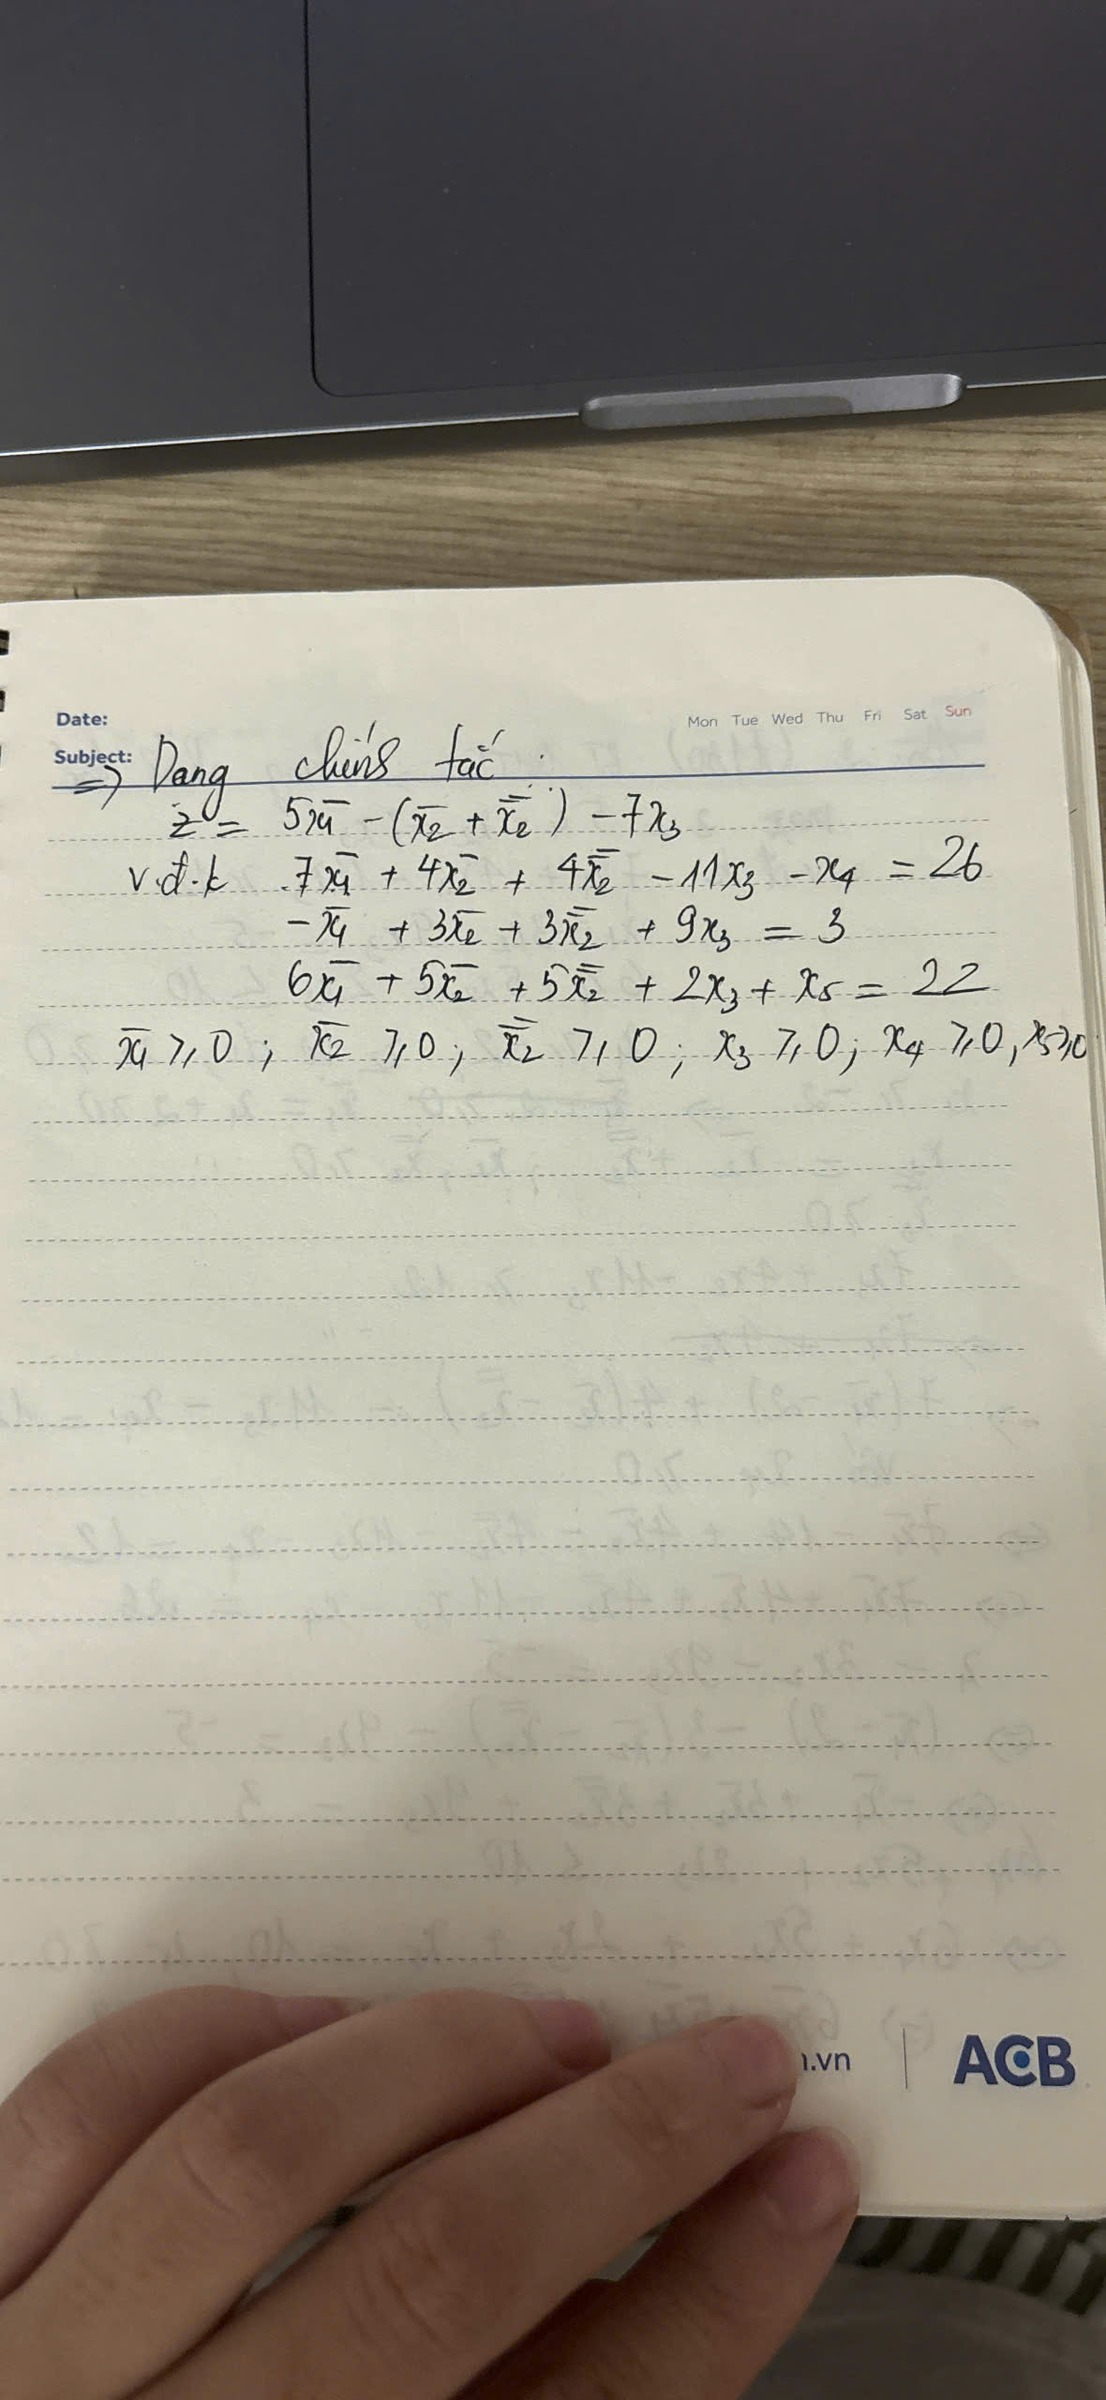
\includegraphics[width=.98\textwidth,height=.82\textheight,keepaspectratio]{bai_lam_them_1_assets/page-001.jpg}\end{center}
\clearpage
\phantomsection\label{src:002}
\noindent\textbf{Ảnh nguồn 002}\par\medskip
\begin{center}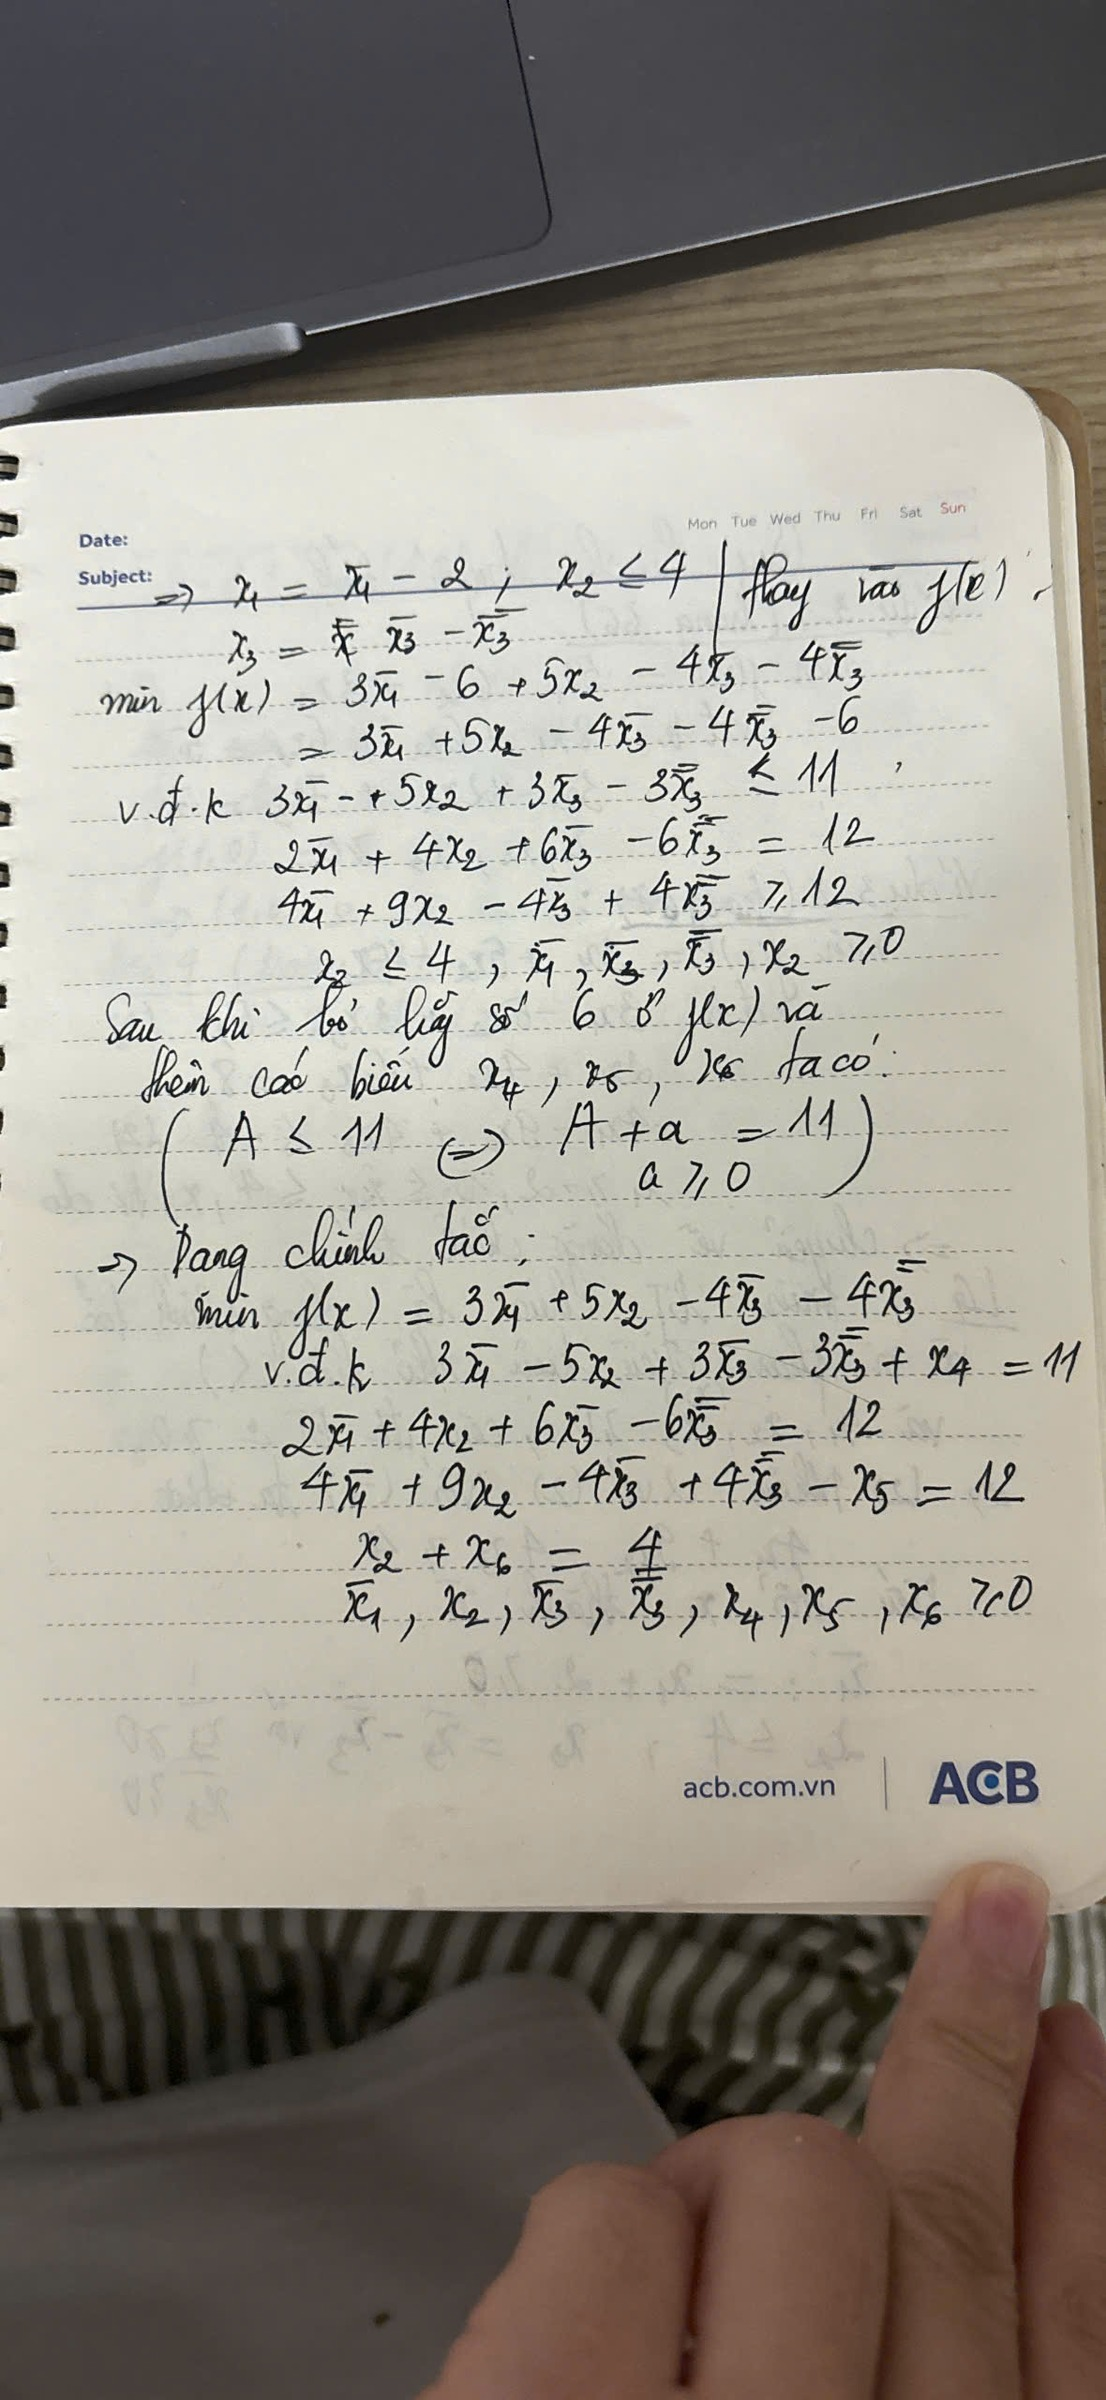
\includegraphics[width=.98\textwidth,height=.82\textheight,keepaspectratio]{bai_lam_them_1_assets/page-002.jpg}\end{center}
\clearpage
\phantomsection\label{src:003}
\noindent\textbf{Ảnh nguồn 003}\par\medskip
\begin{center}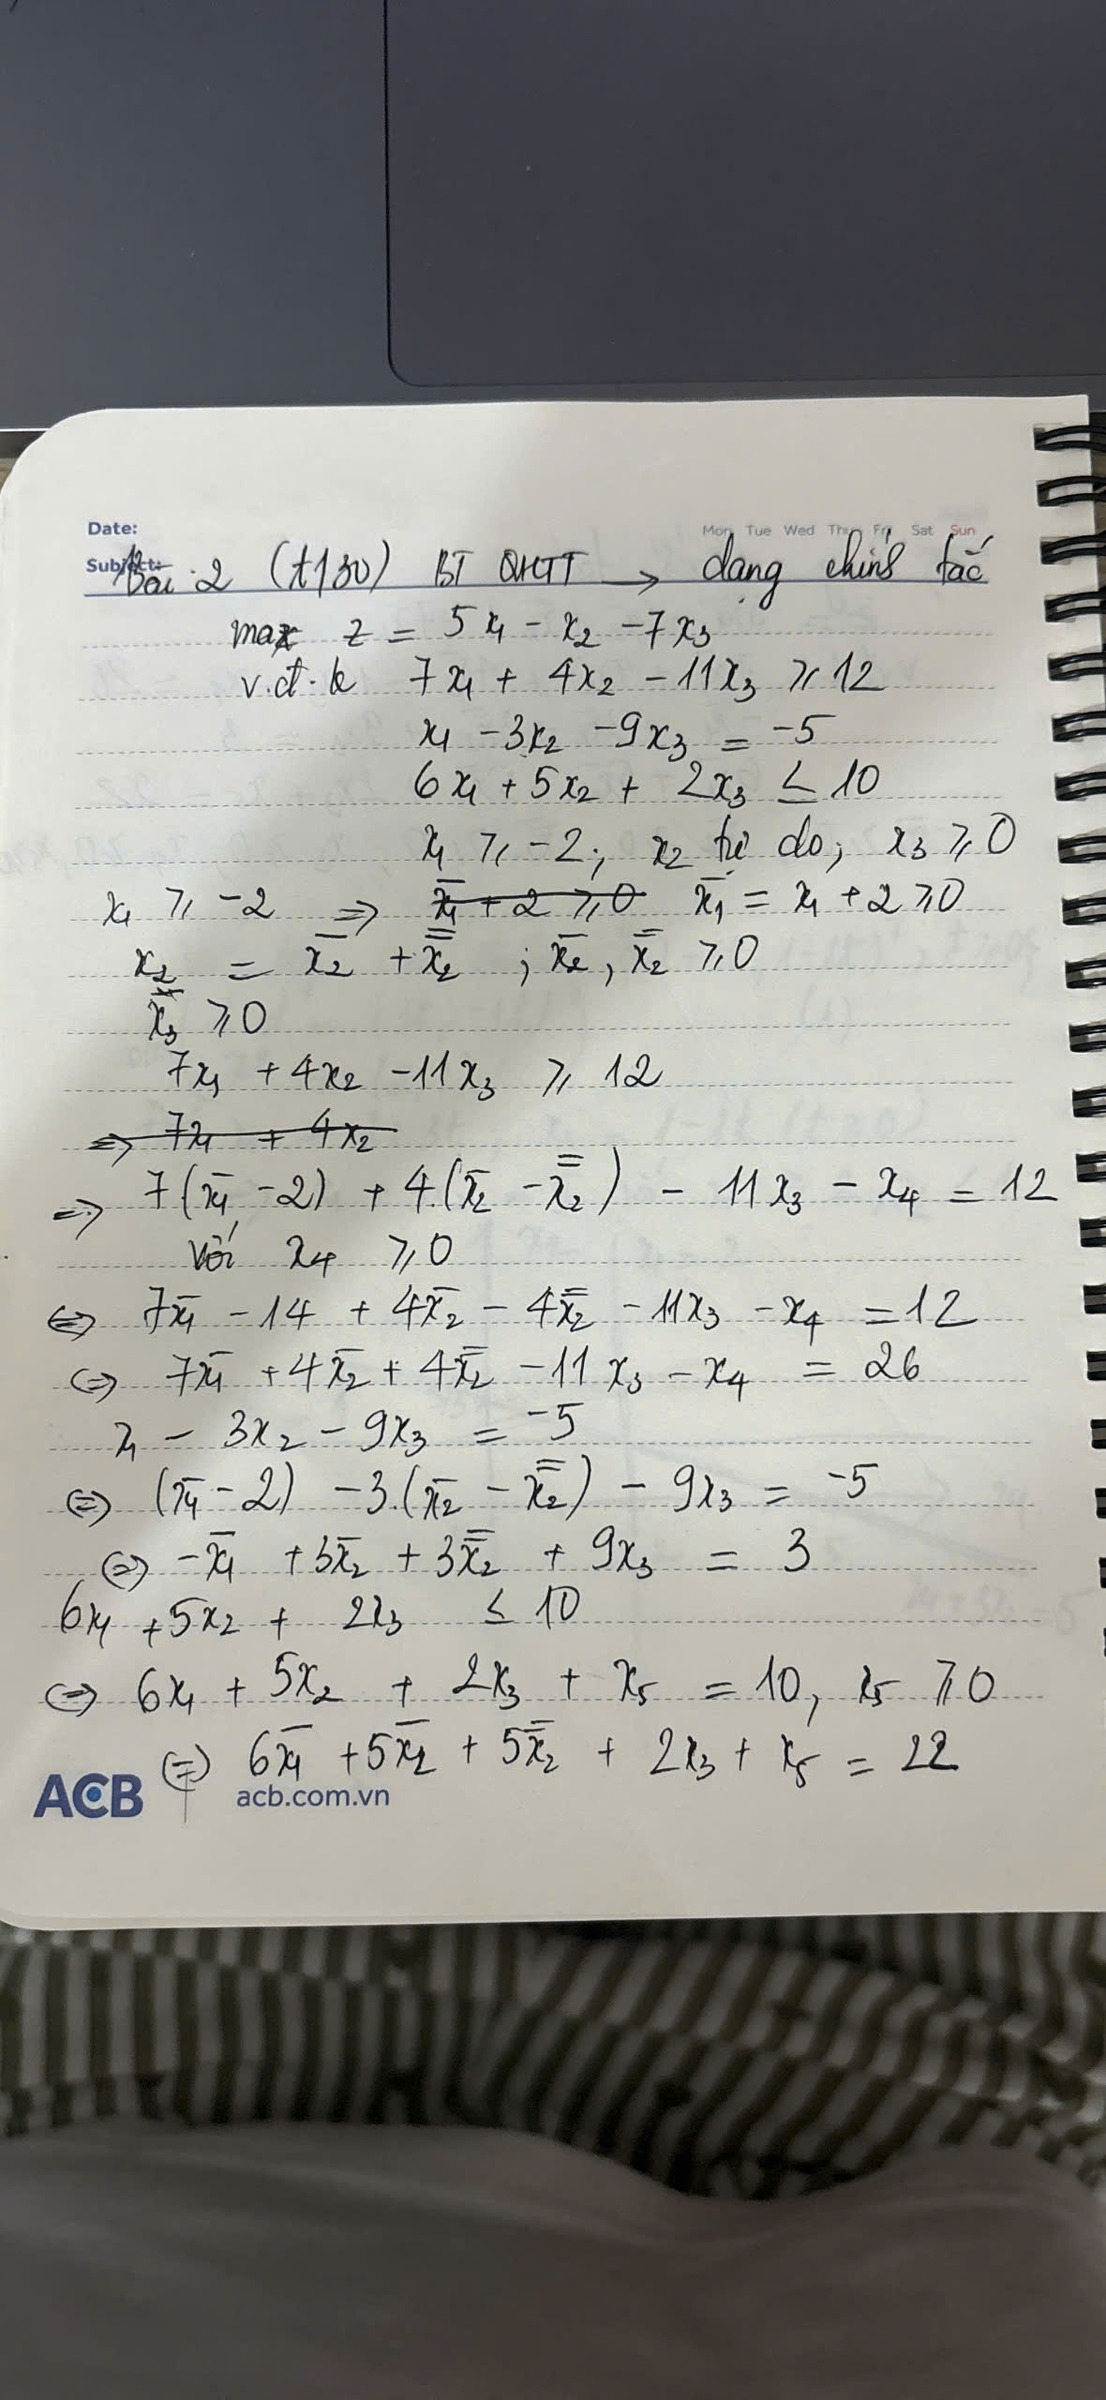
\includegraphics[width=.98\textwidth,height=.82\textheight,keepaspectratio]{bai_lam_them_1_assets/page-003.jpg}\end{center}
\clearpage
\phantomsection\label{src:004}
\noindent\textbf{Ảnh nguồn 004}\par\medskip
\begin{center}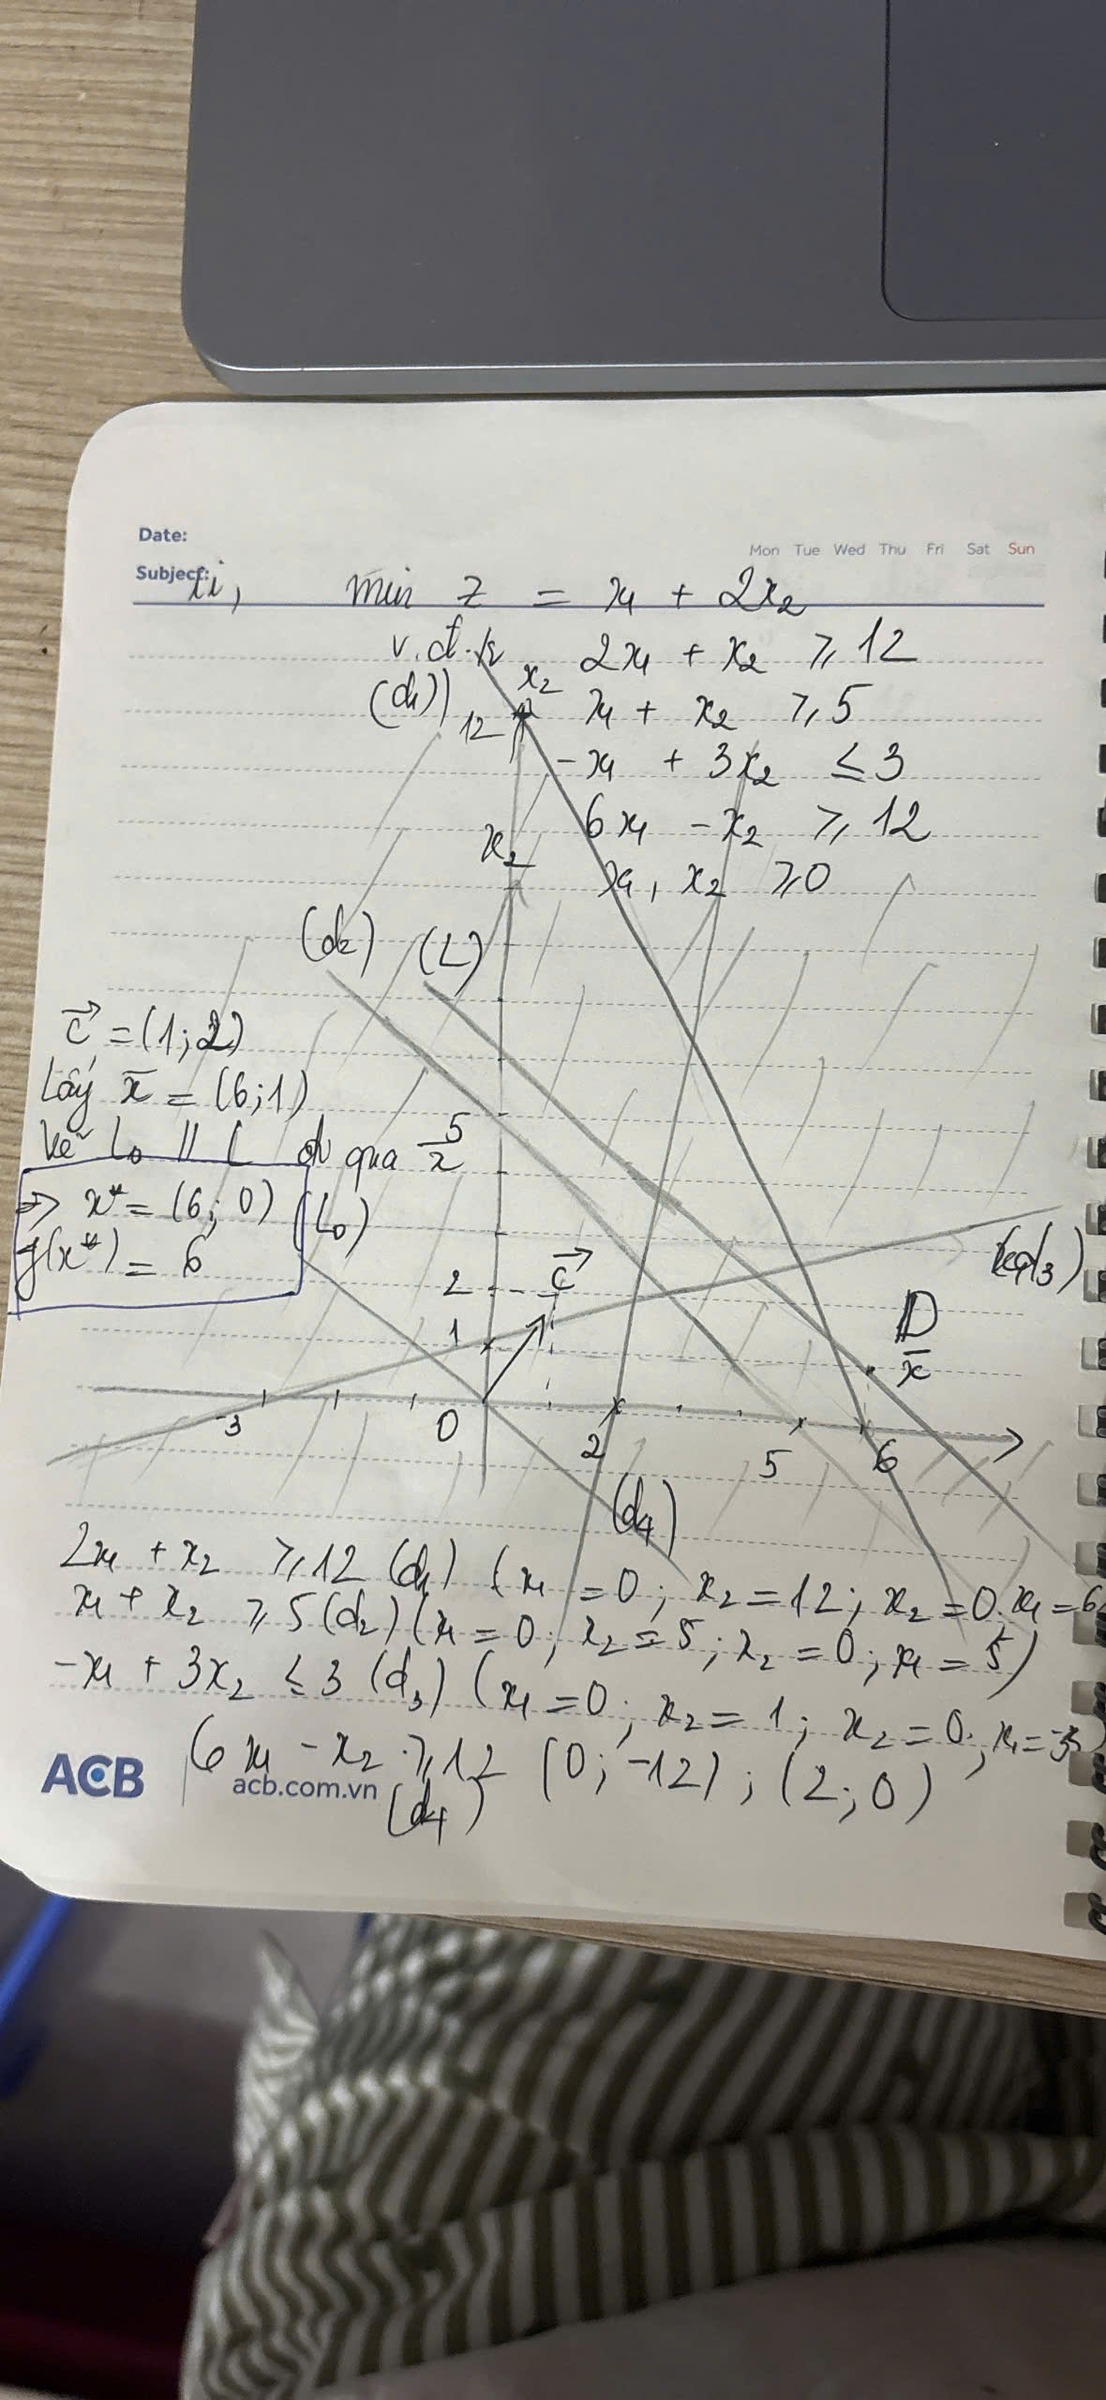
\includegraphics[width=.98\textwidth,height=.82\textheight,keepaspectratio]{bai_lam_them_1_assets/page-004.jpg}\end{center}
\clearpage
\phantomsection\label{src:005}
\noindent\textbf{Ảnh nguồn 005}\par\medskip
\begin{center}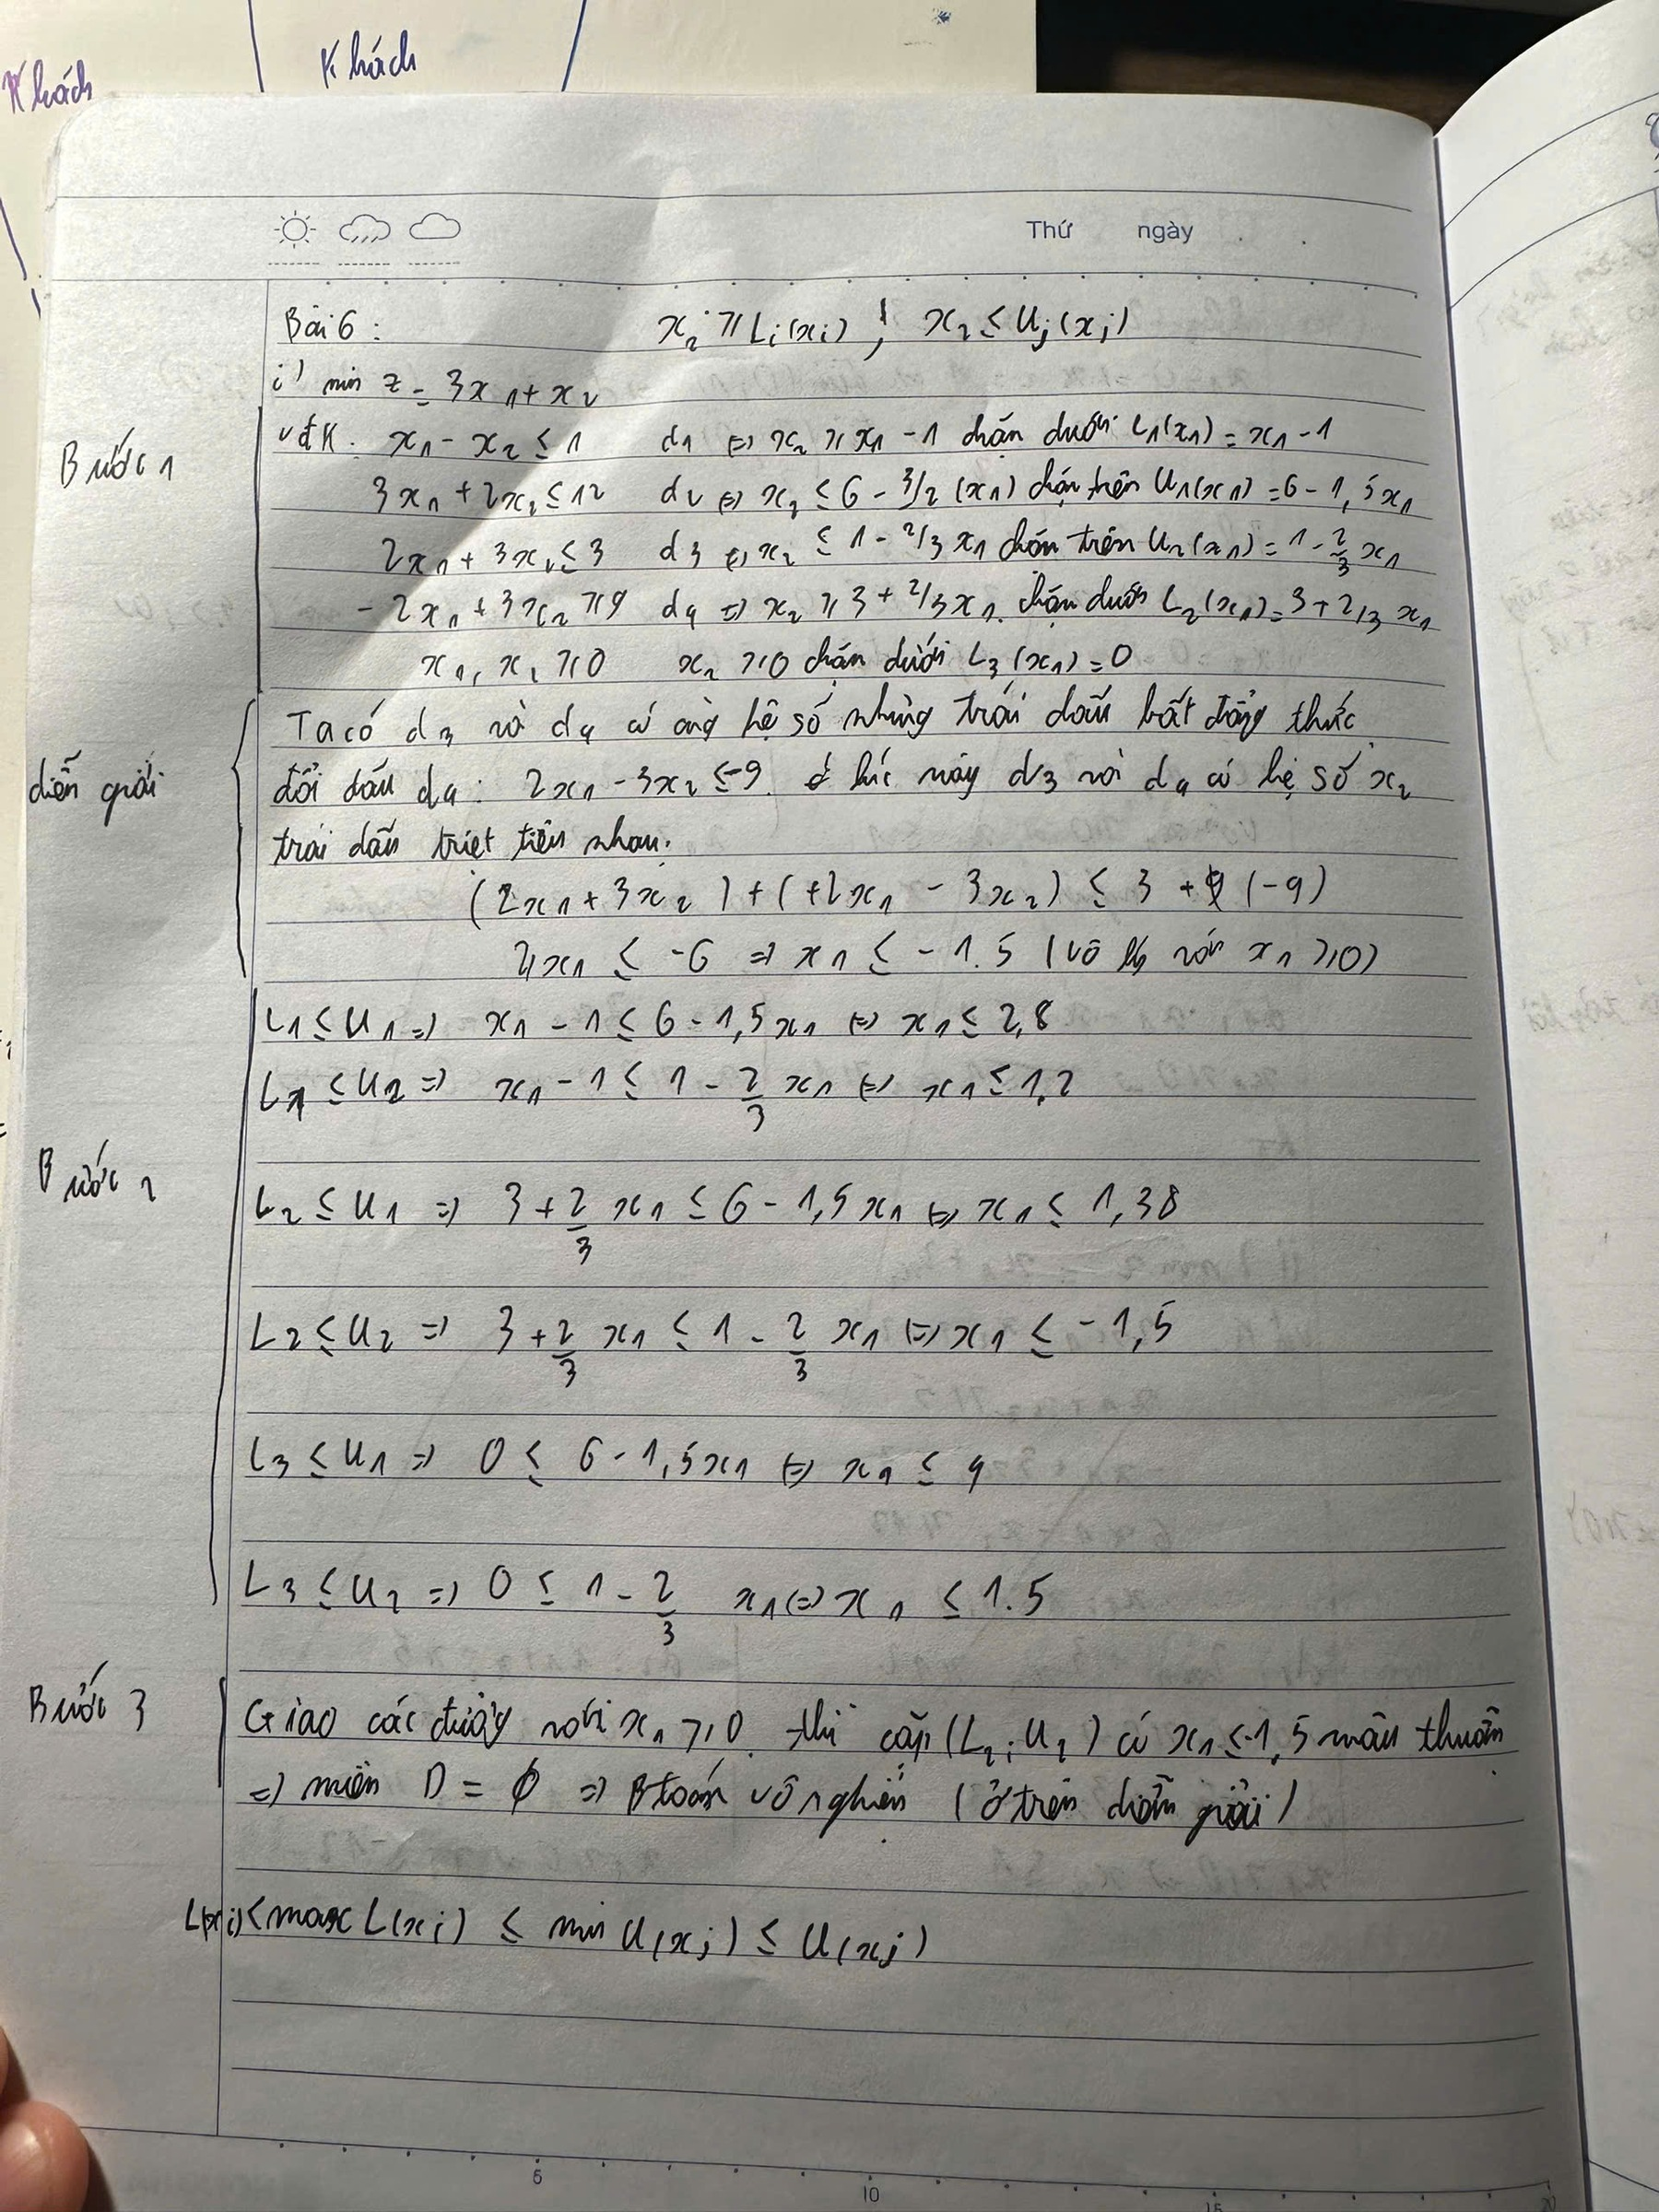
\includegraphics[width=.98\textwidth,height=.82\textheight,keepaspectratio]{bai_lam_them_1_assets/page-005.jpg}\end{center}
\clearpage
\phantomsection\label{src:006}
\noindent\textbf{Ảnh nguồn 006}\par\medskip
\begin{center}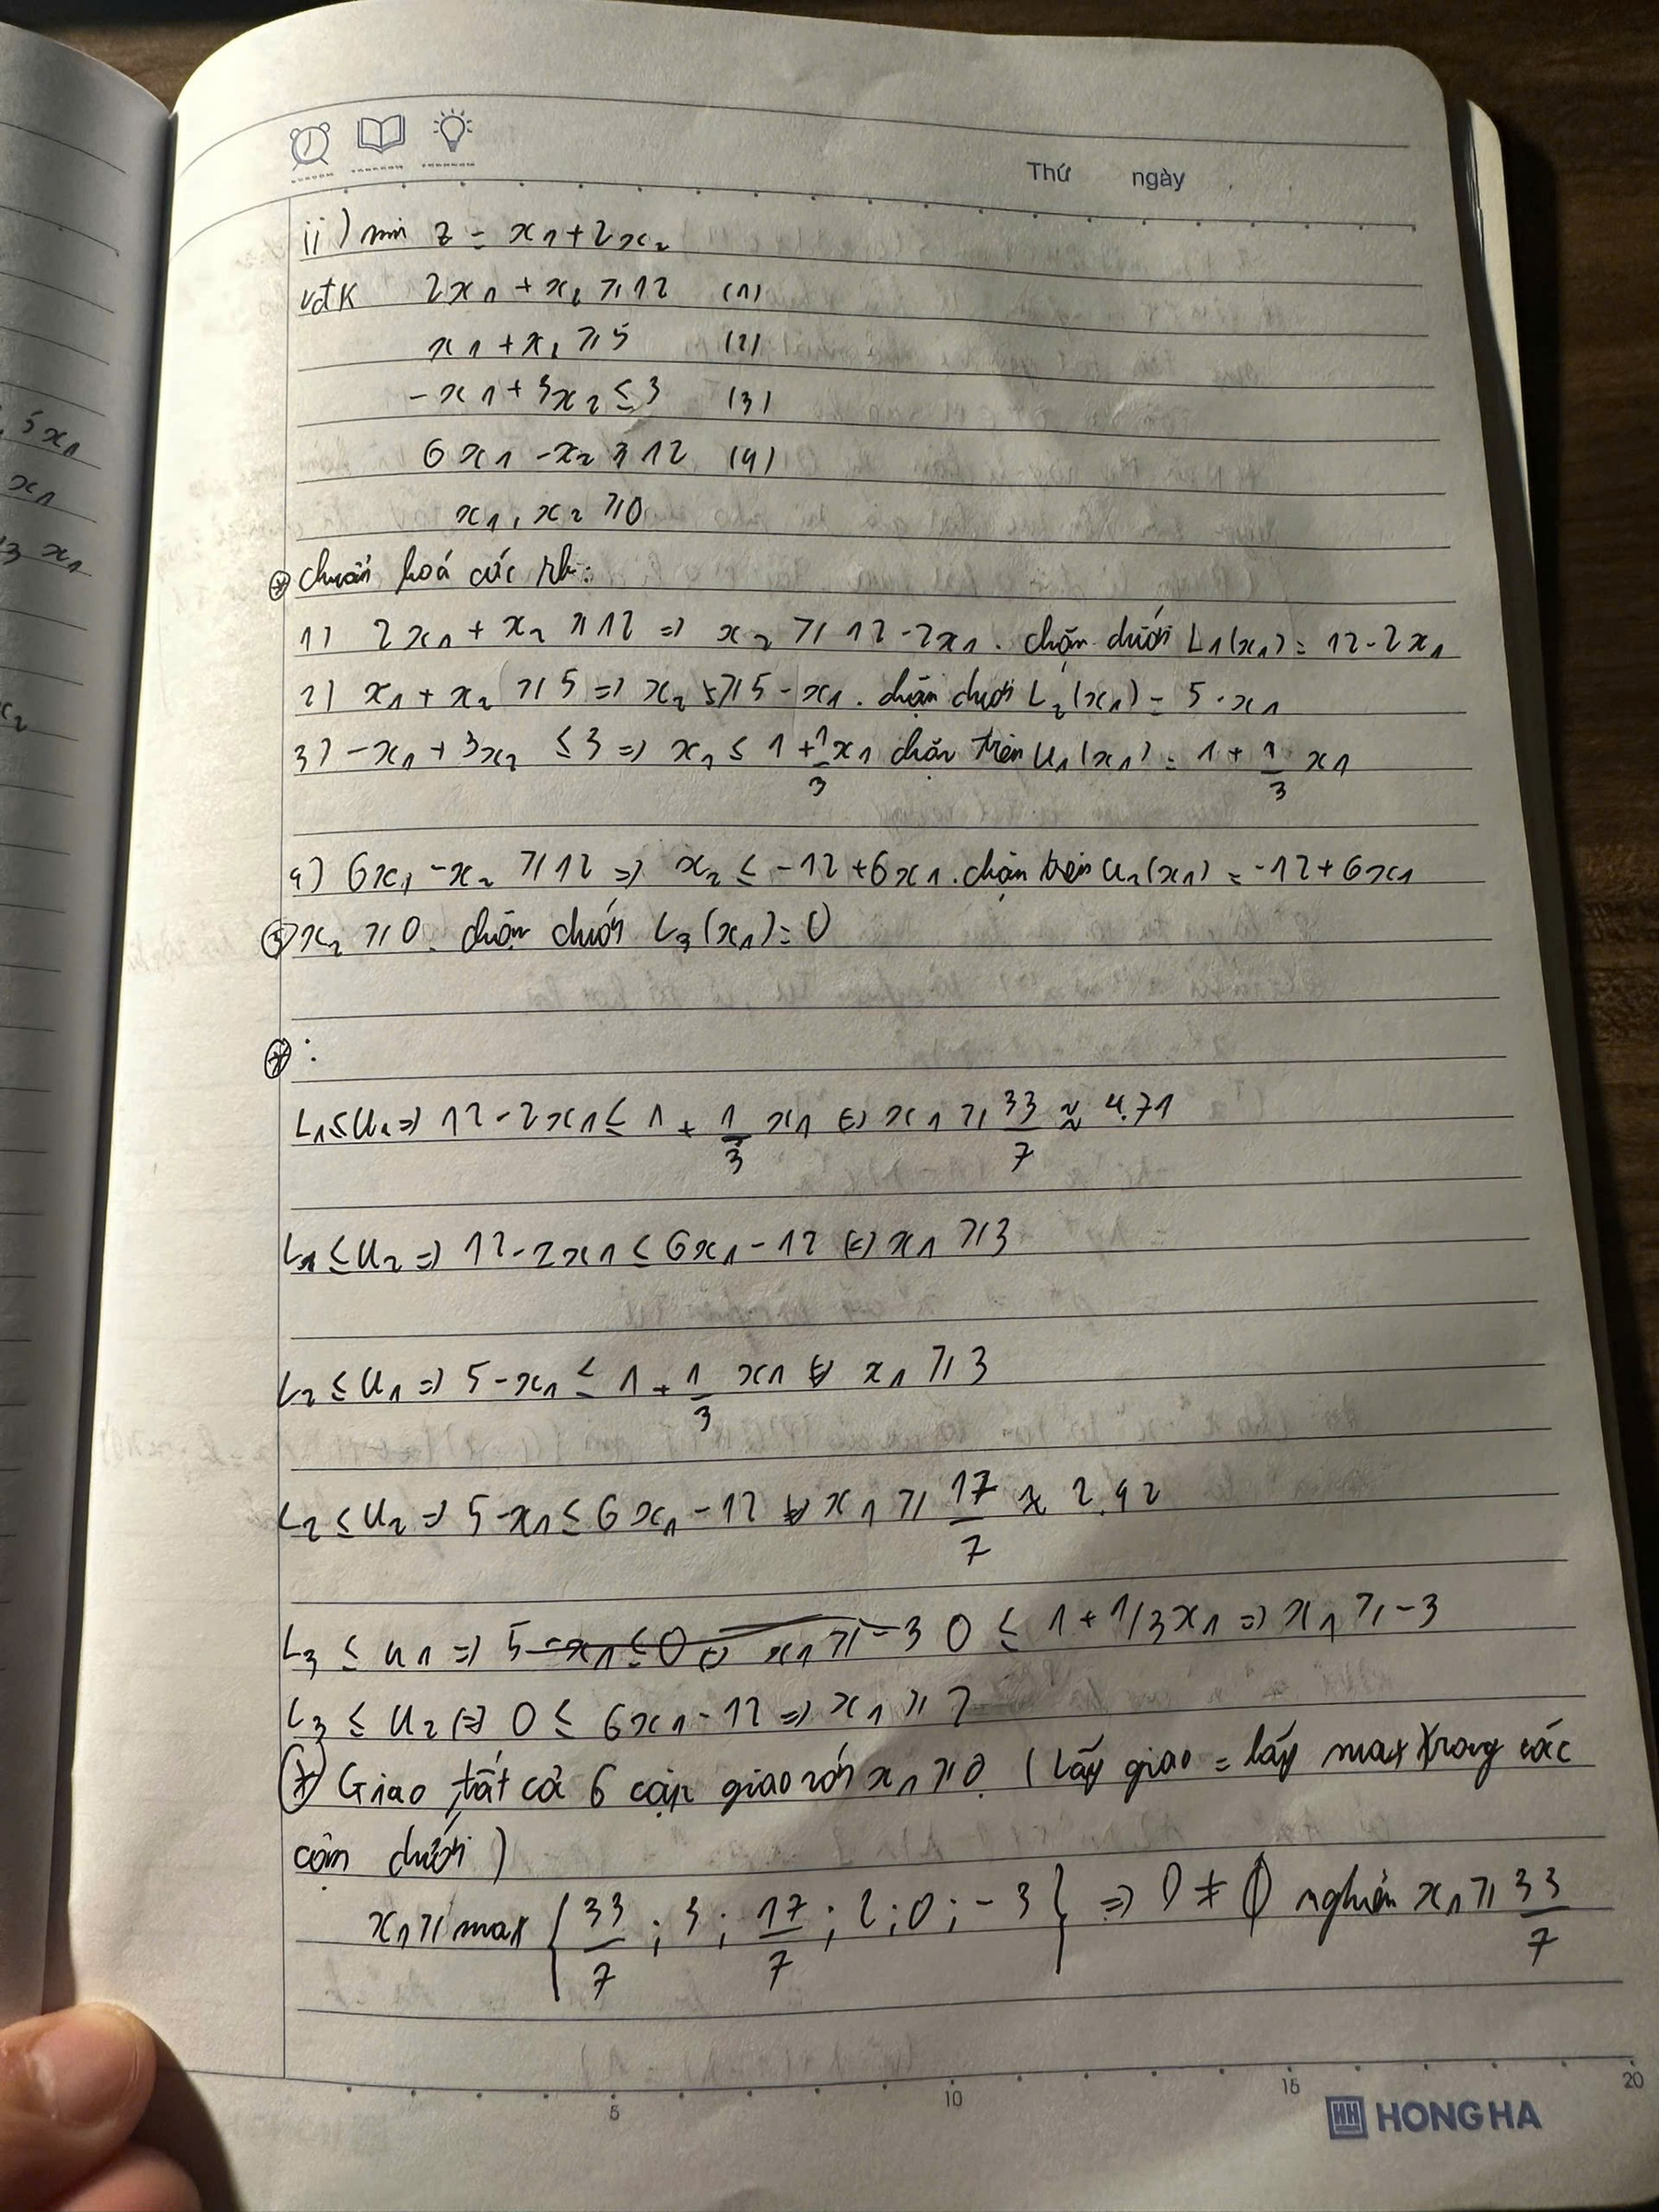
\includegraphics[width=.98\textwidth,height=.82\textheight,keepaspectratio]{bai_lam_them_1_assets/page-006.jpg}\end{center}
\clearpage
\phantomsection\label{src:007}
\noindent\textbf{Ảnh nguồn 007}\par\medskip
\begin{center}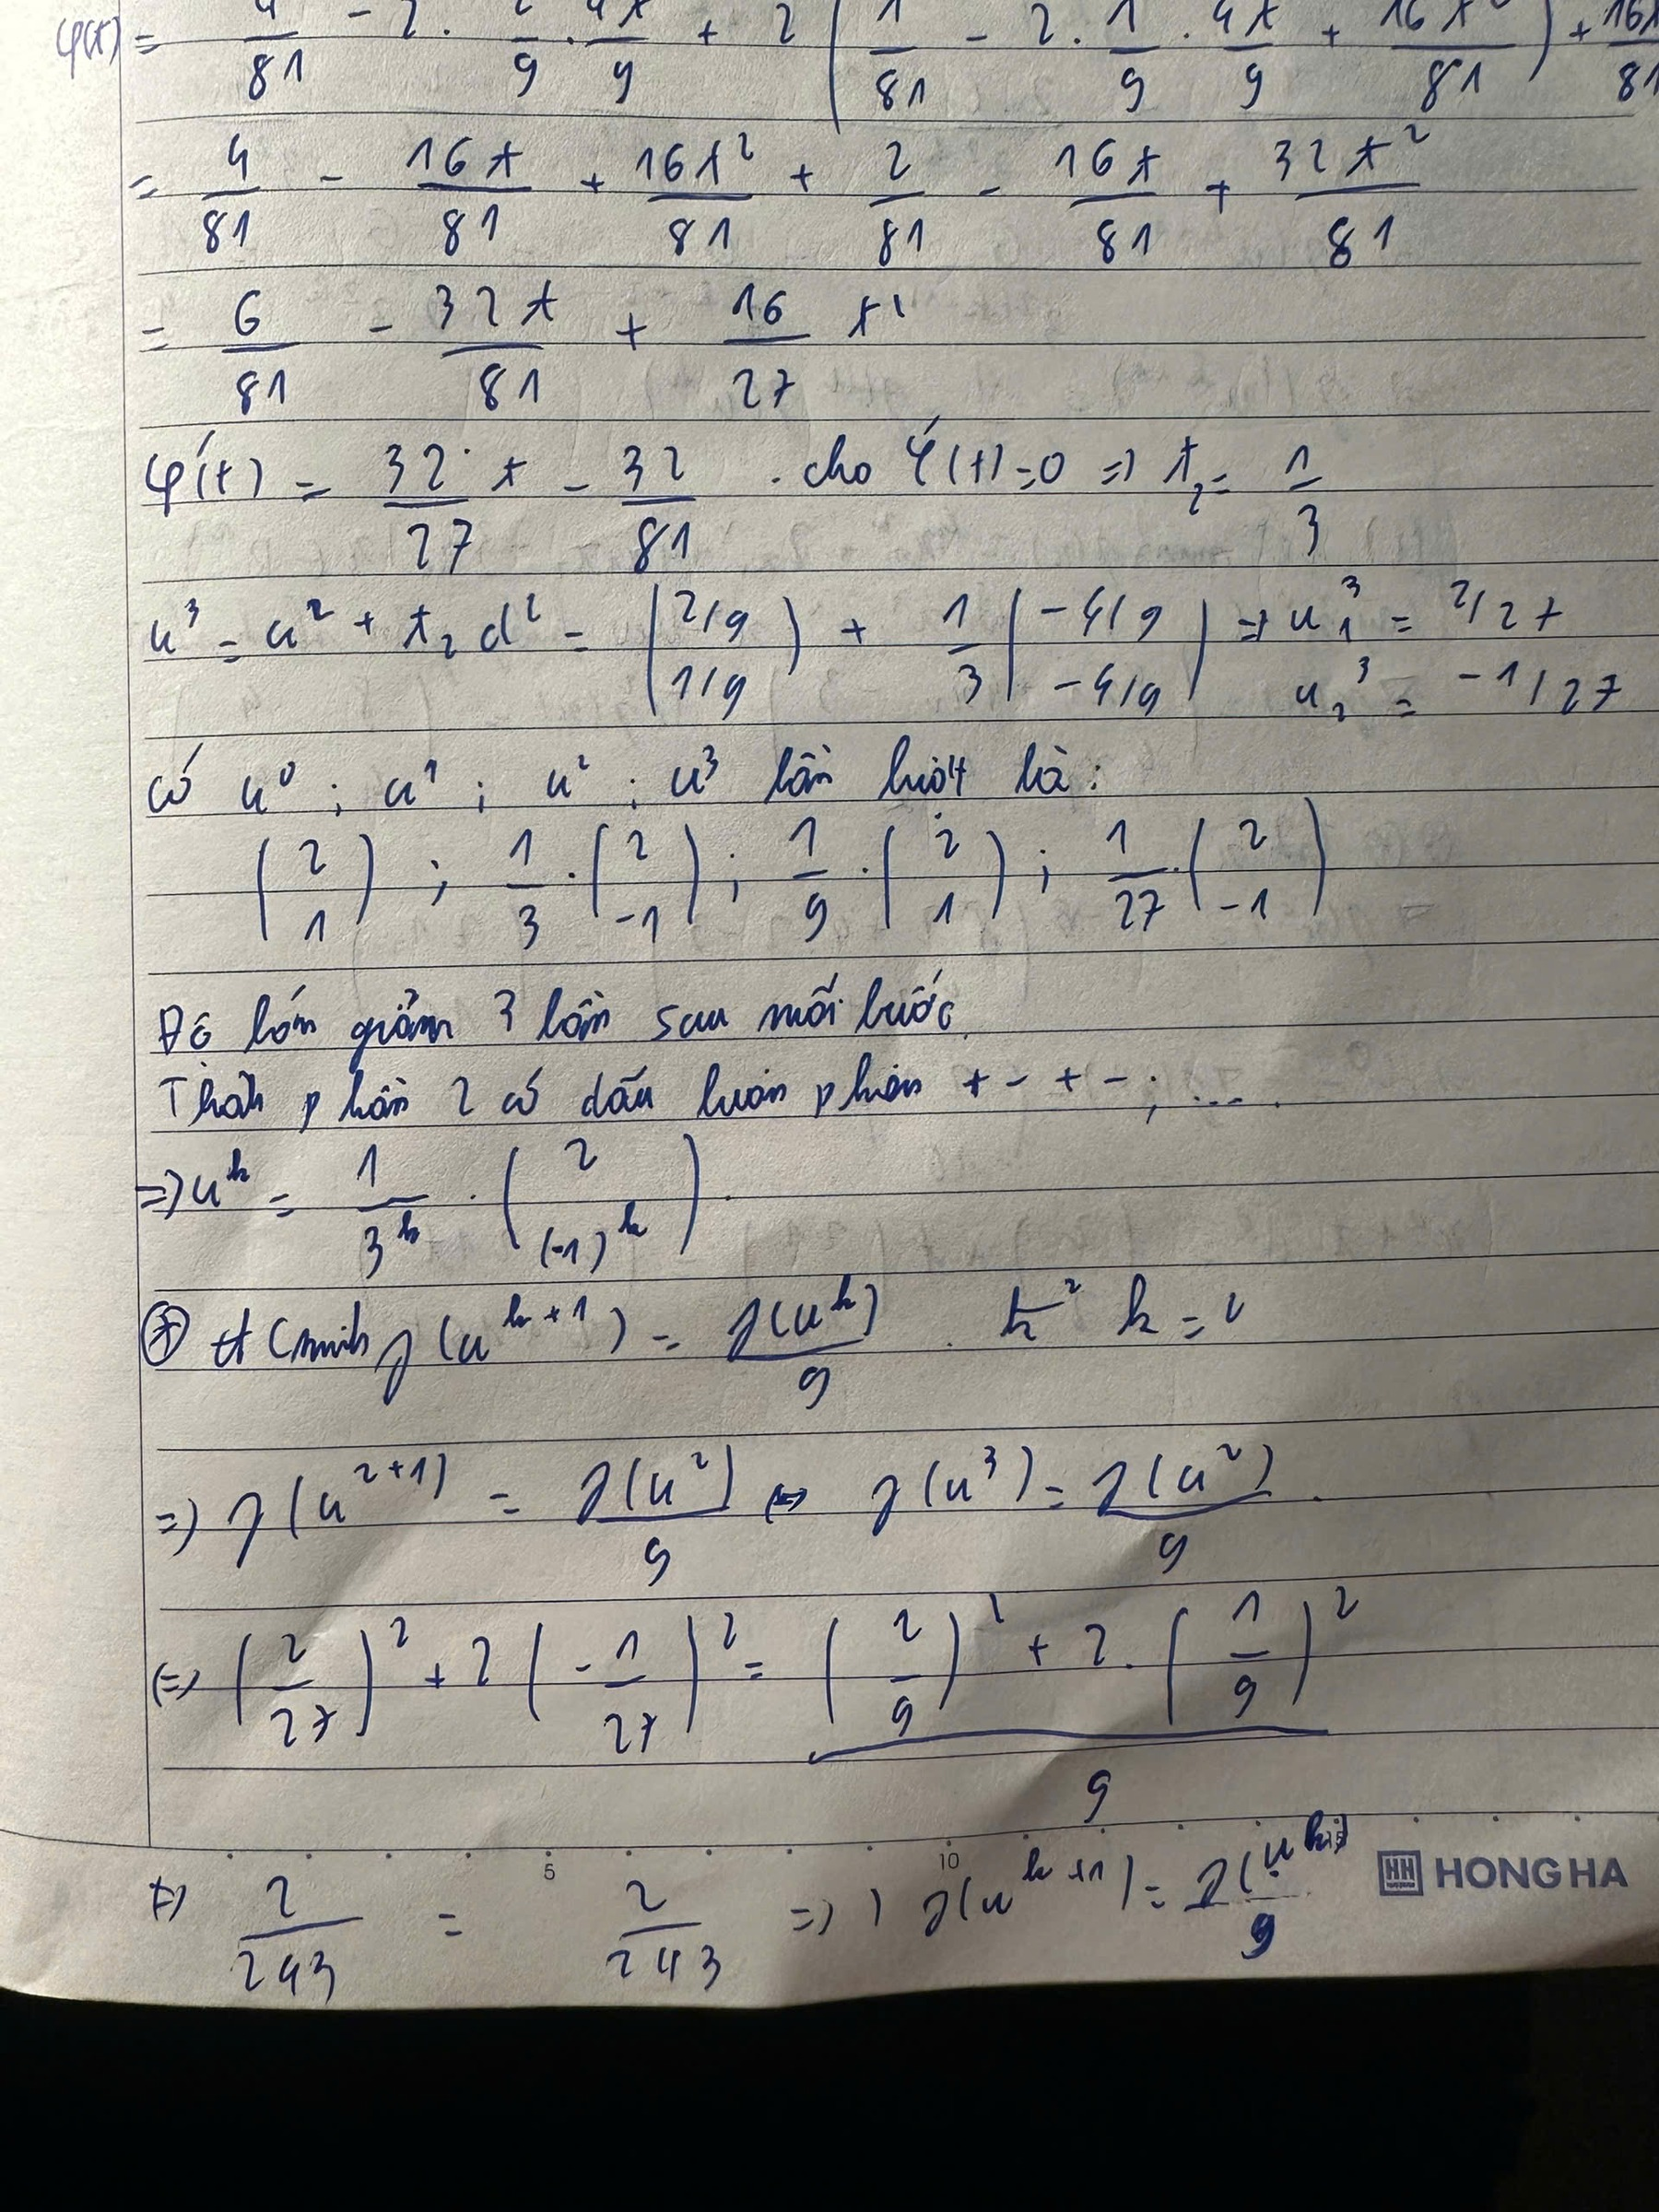
\includegraphics[width=.98\textwidth,height=.82\textheight,keepaspectratio]{bai_lam_them_1_assets/page-007.jpg}\end{center}
\clearpage
\phantomsection\label{src:008}
\noindent\textbf{Ảnh nguồn 008}\par\medskip
\begin{center}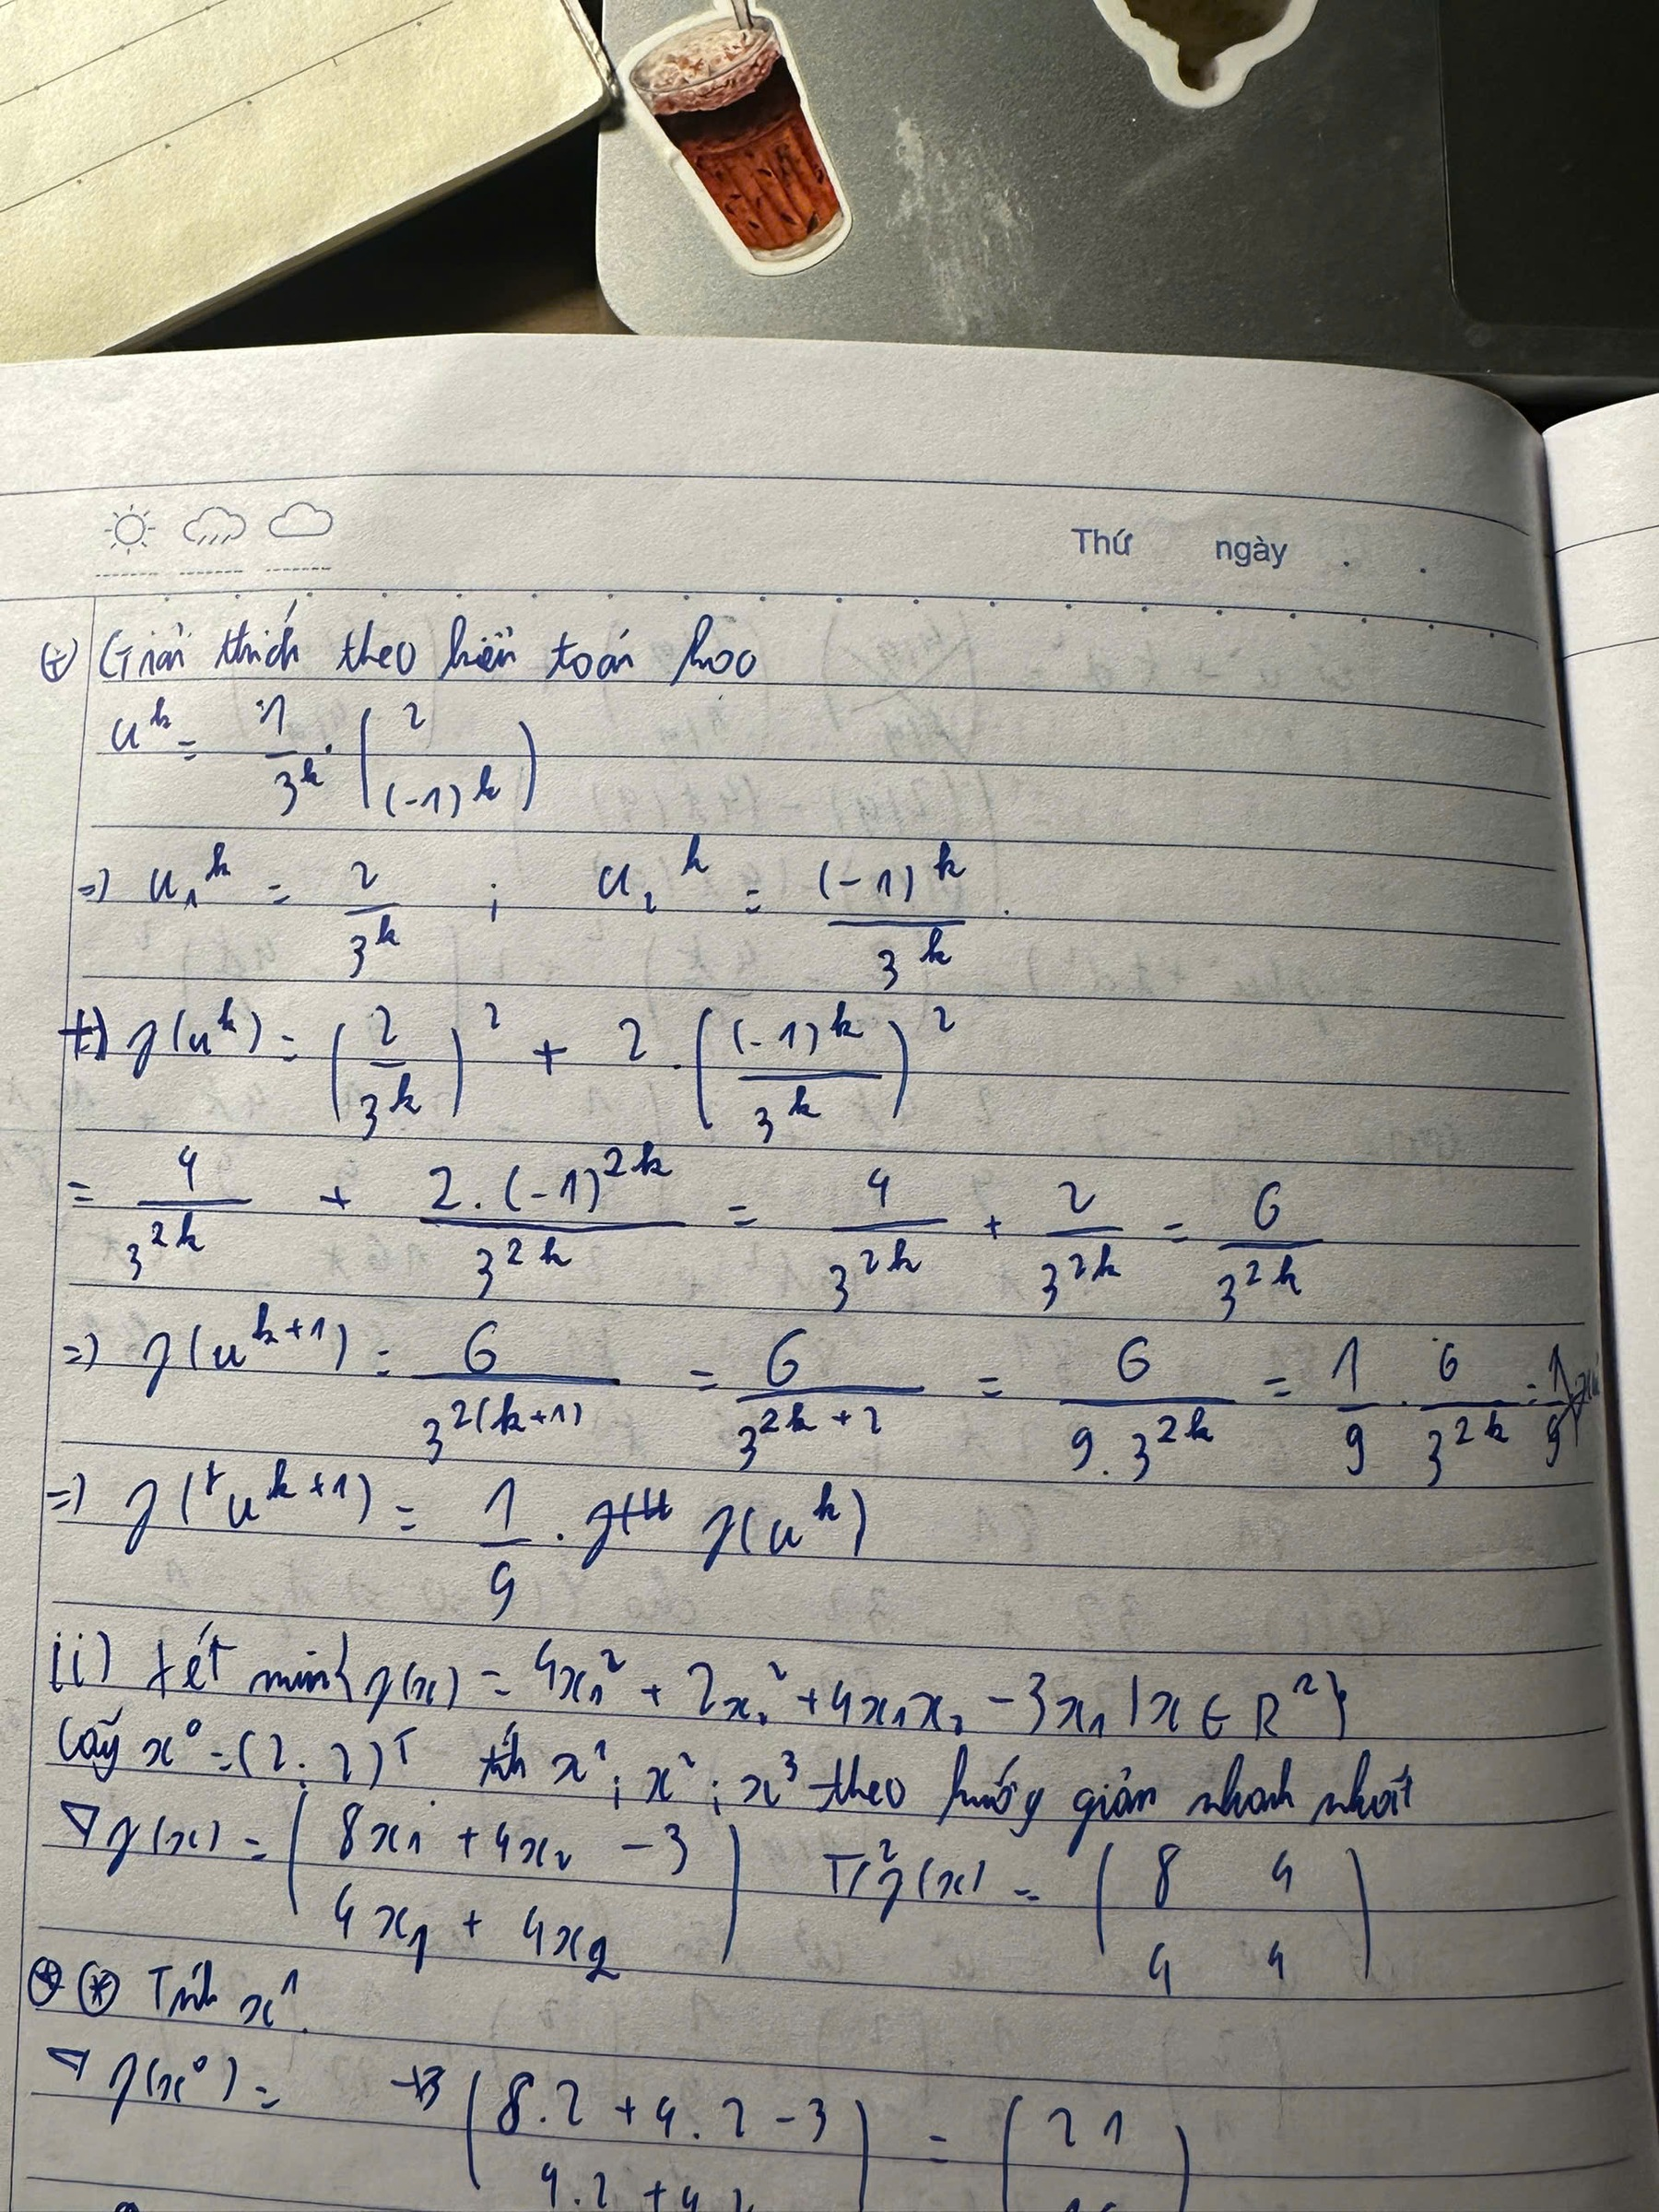
\includegraphics[width=.98\textwidth,height=.82\textheight,keepaspectratio]{bai_lam_them_1_assets/page-008.jpg}\end{center}
\clearpage
\phantomsection\label{src:009}
\noindent\textbf{Ảnh nguồn 009}\par\medskip
\begin{center}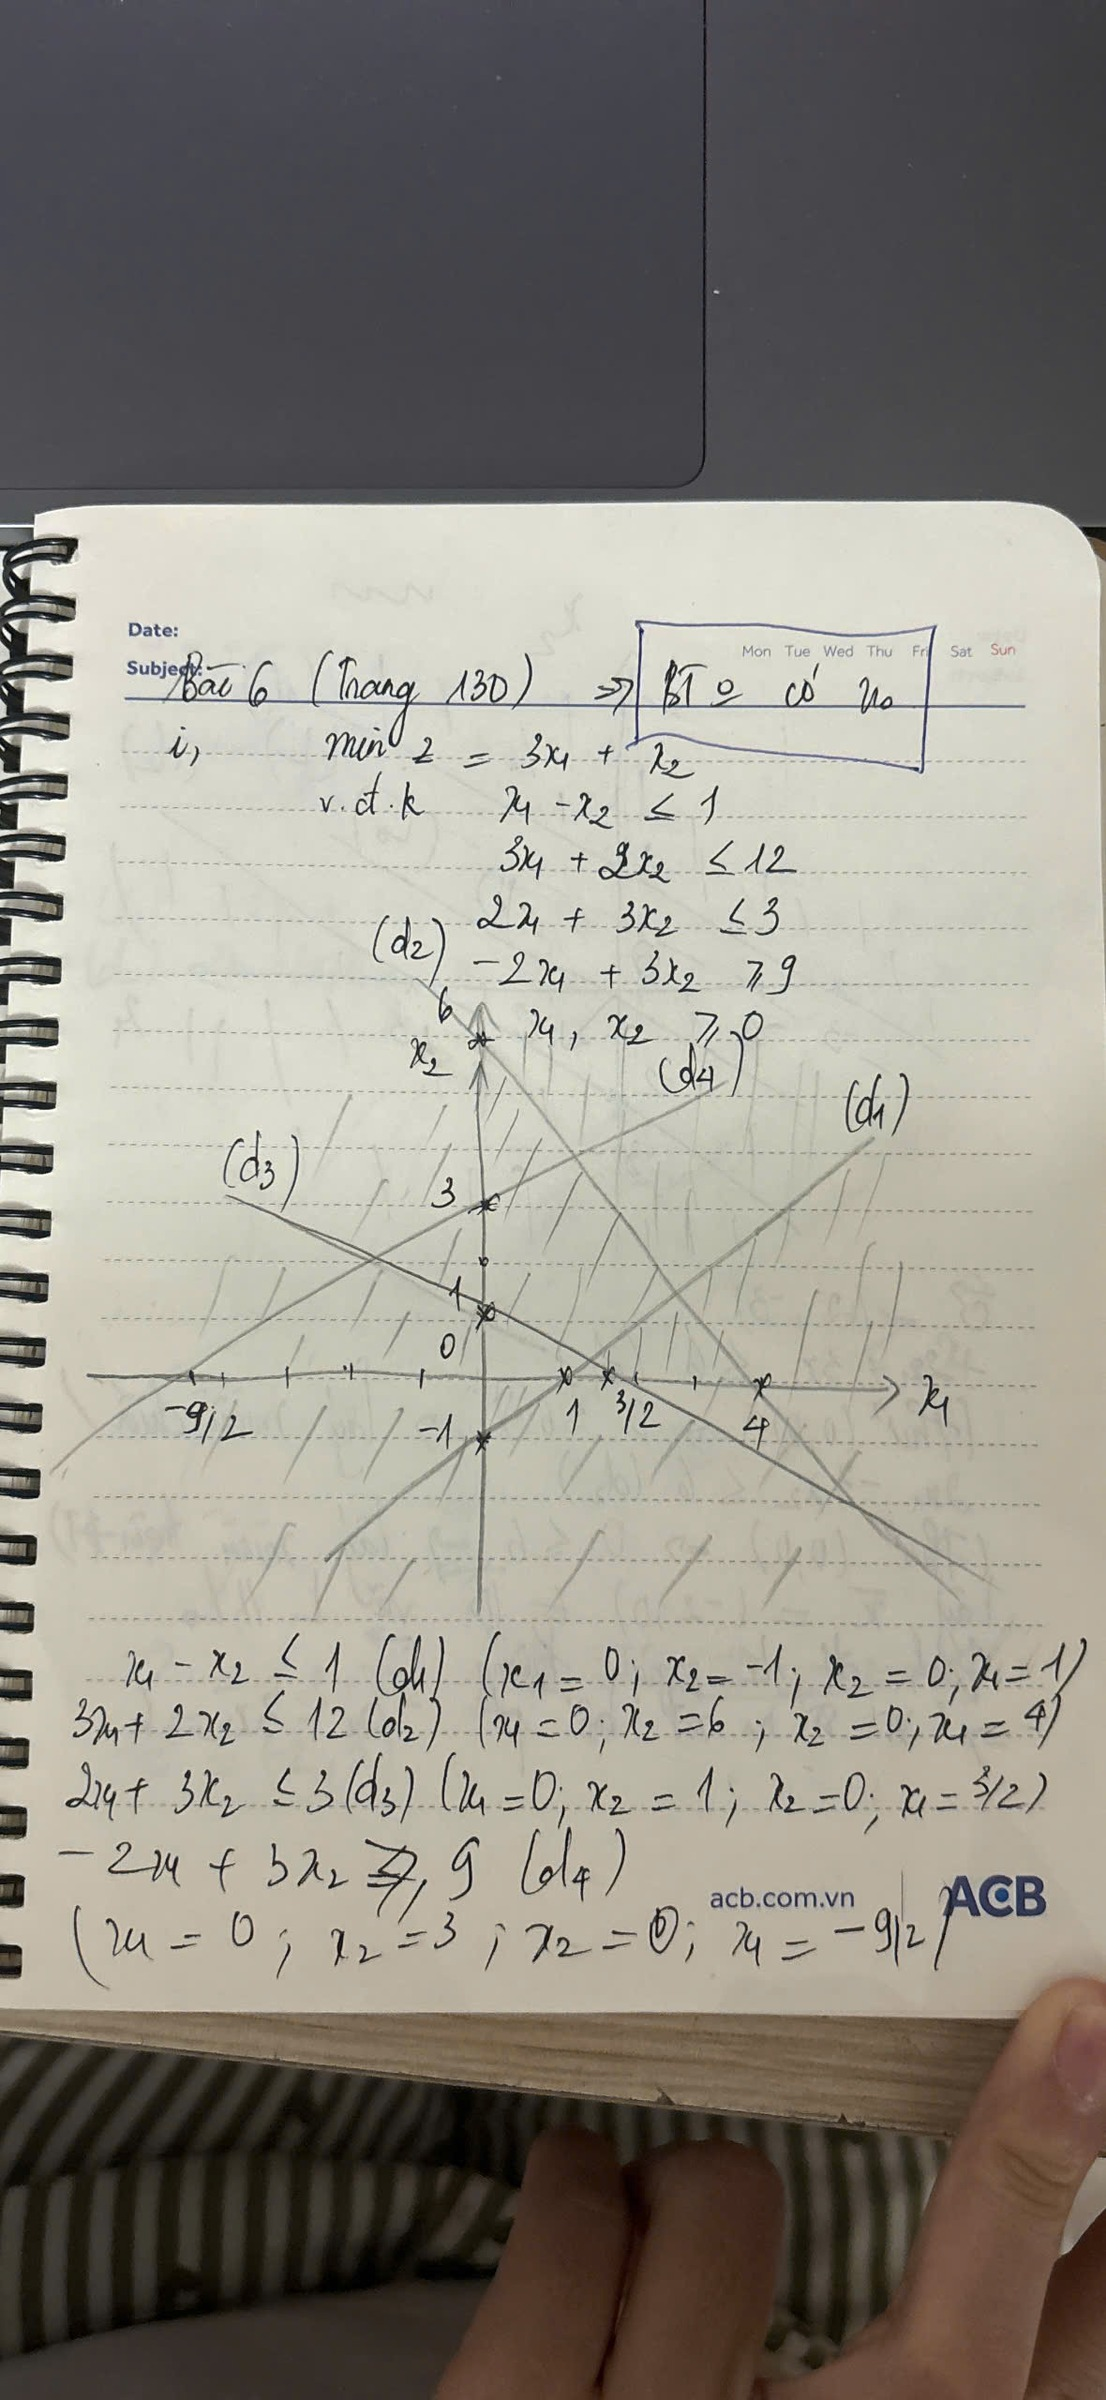
\includegraphics[width=.98\textwidth,height=.82\textheight,keepaspectratio]{bai_lam_them_1_assets/page-009.jpg}\end{center}
\clearpage
\phantomsection\label{src:010}
\noindent\textbf{Ảnh nguồn 010}\par\medskip
\begin{center}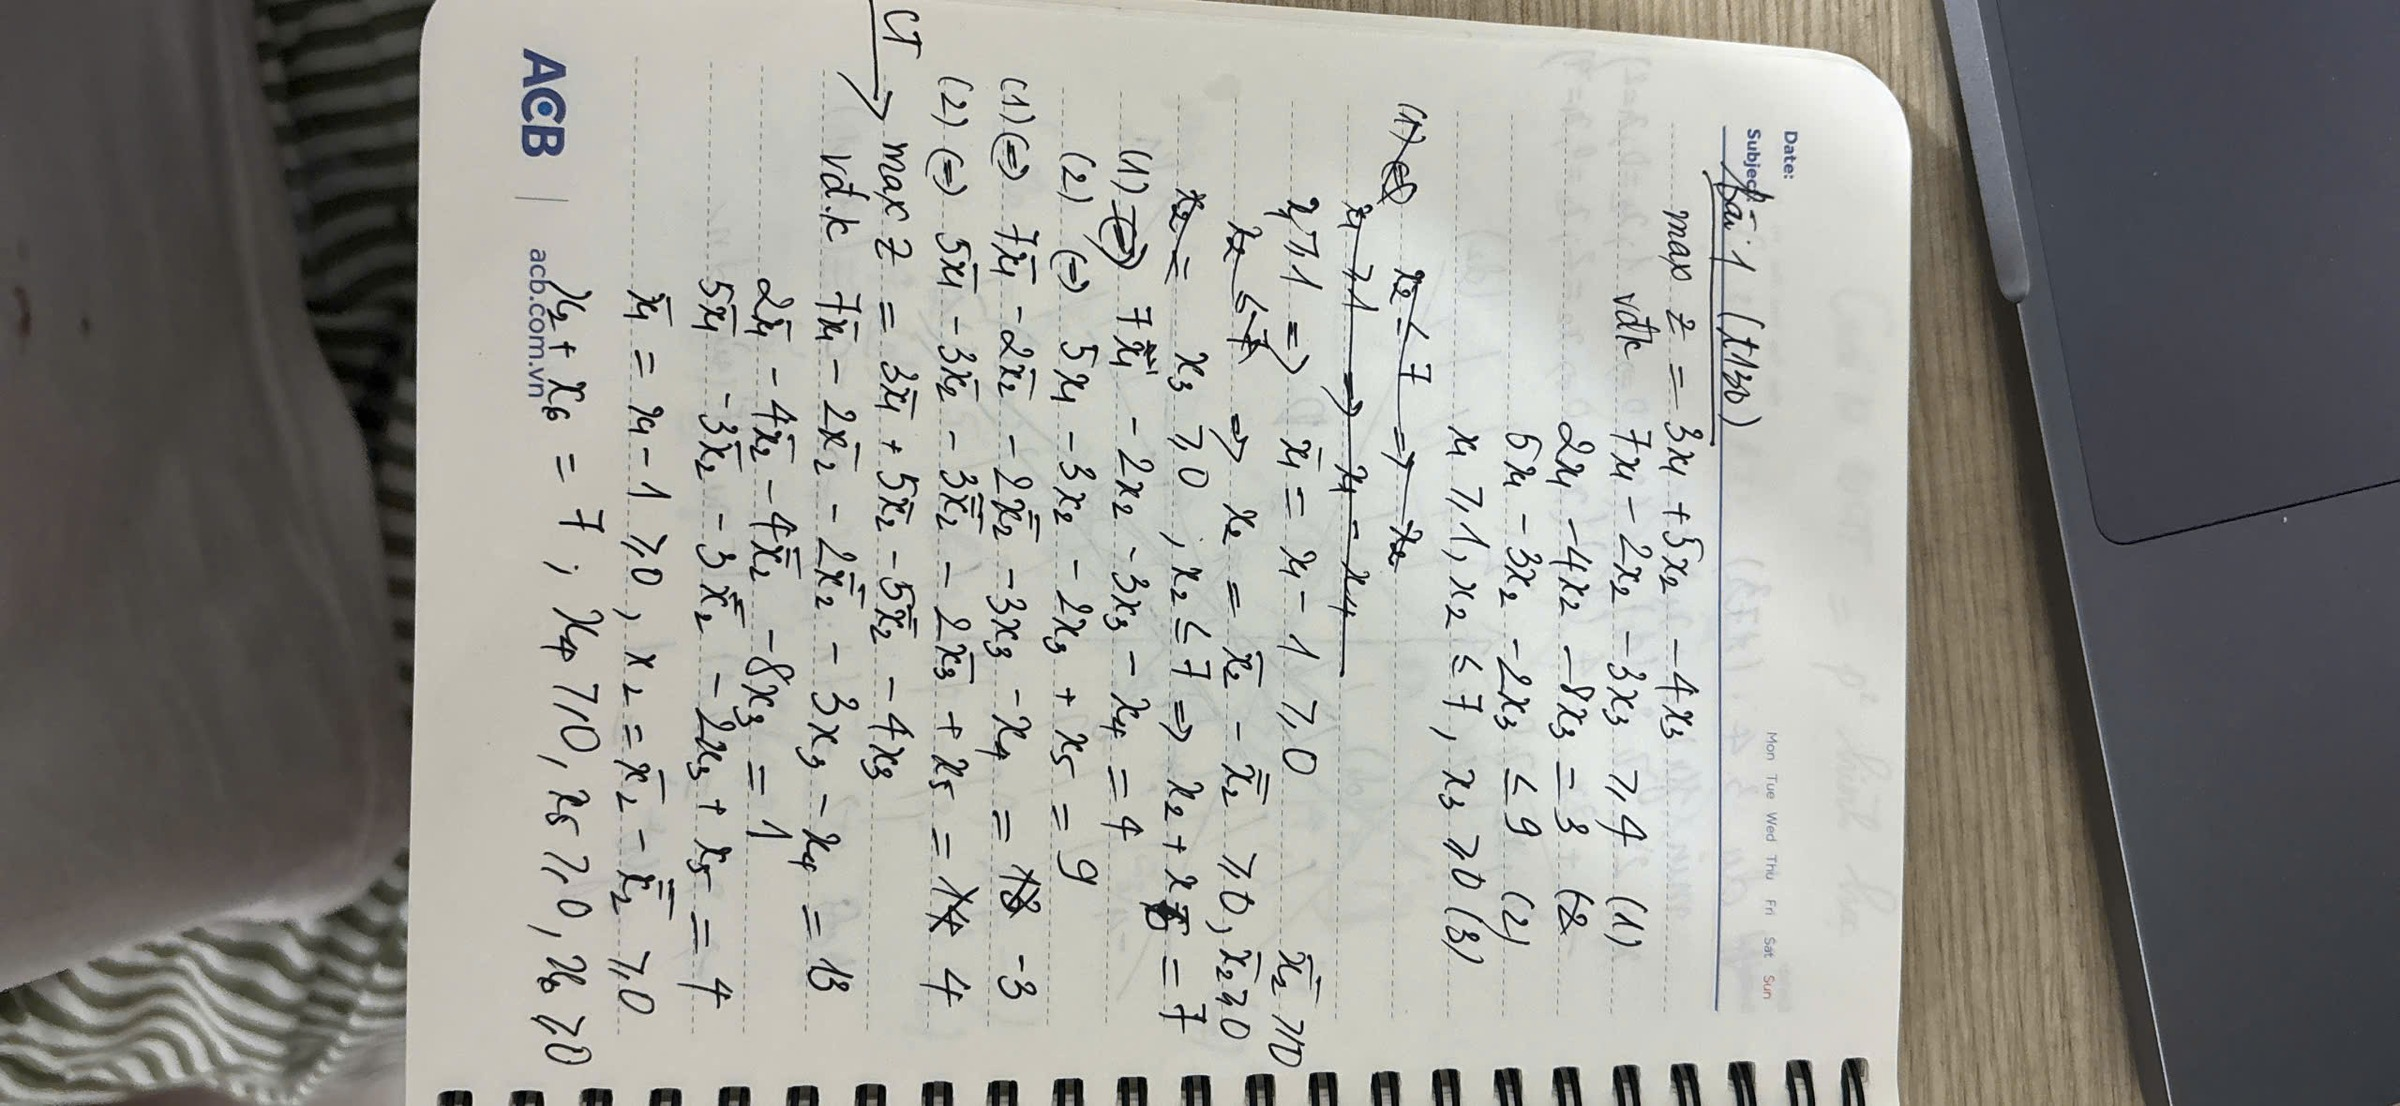
\includegraphics[width=.98\textwidth,height=.82\textheight,keepaspectratio]{bai_lam_them_1_assets/page-010.jpg}\end{center}
\clearpage
\phantomsection\label{src:011}
\noindent\textbf{Ảnh nguồn 011}\par\medskip
\begin{center}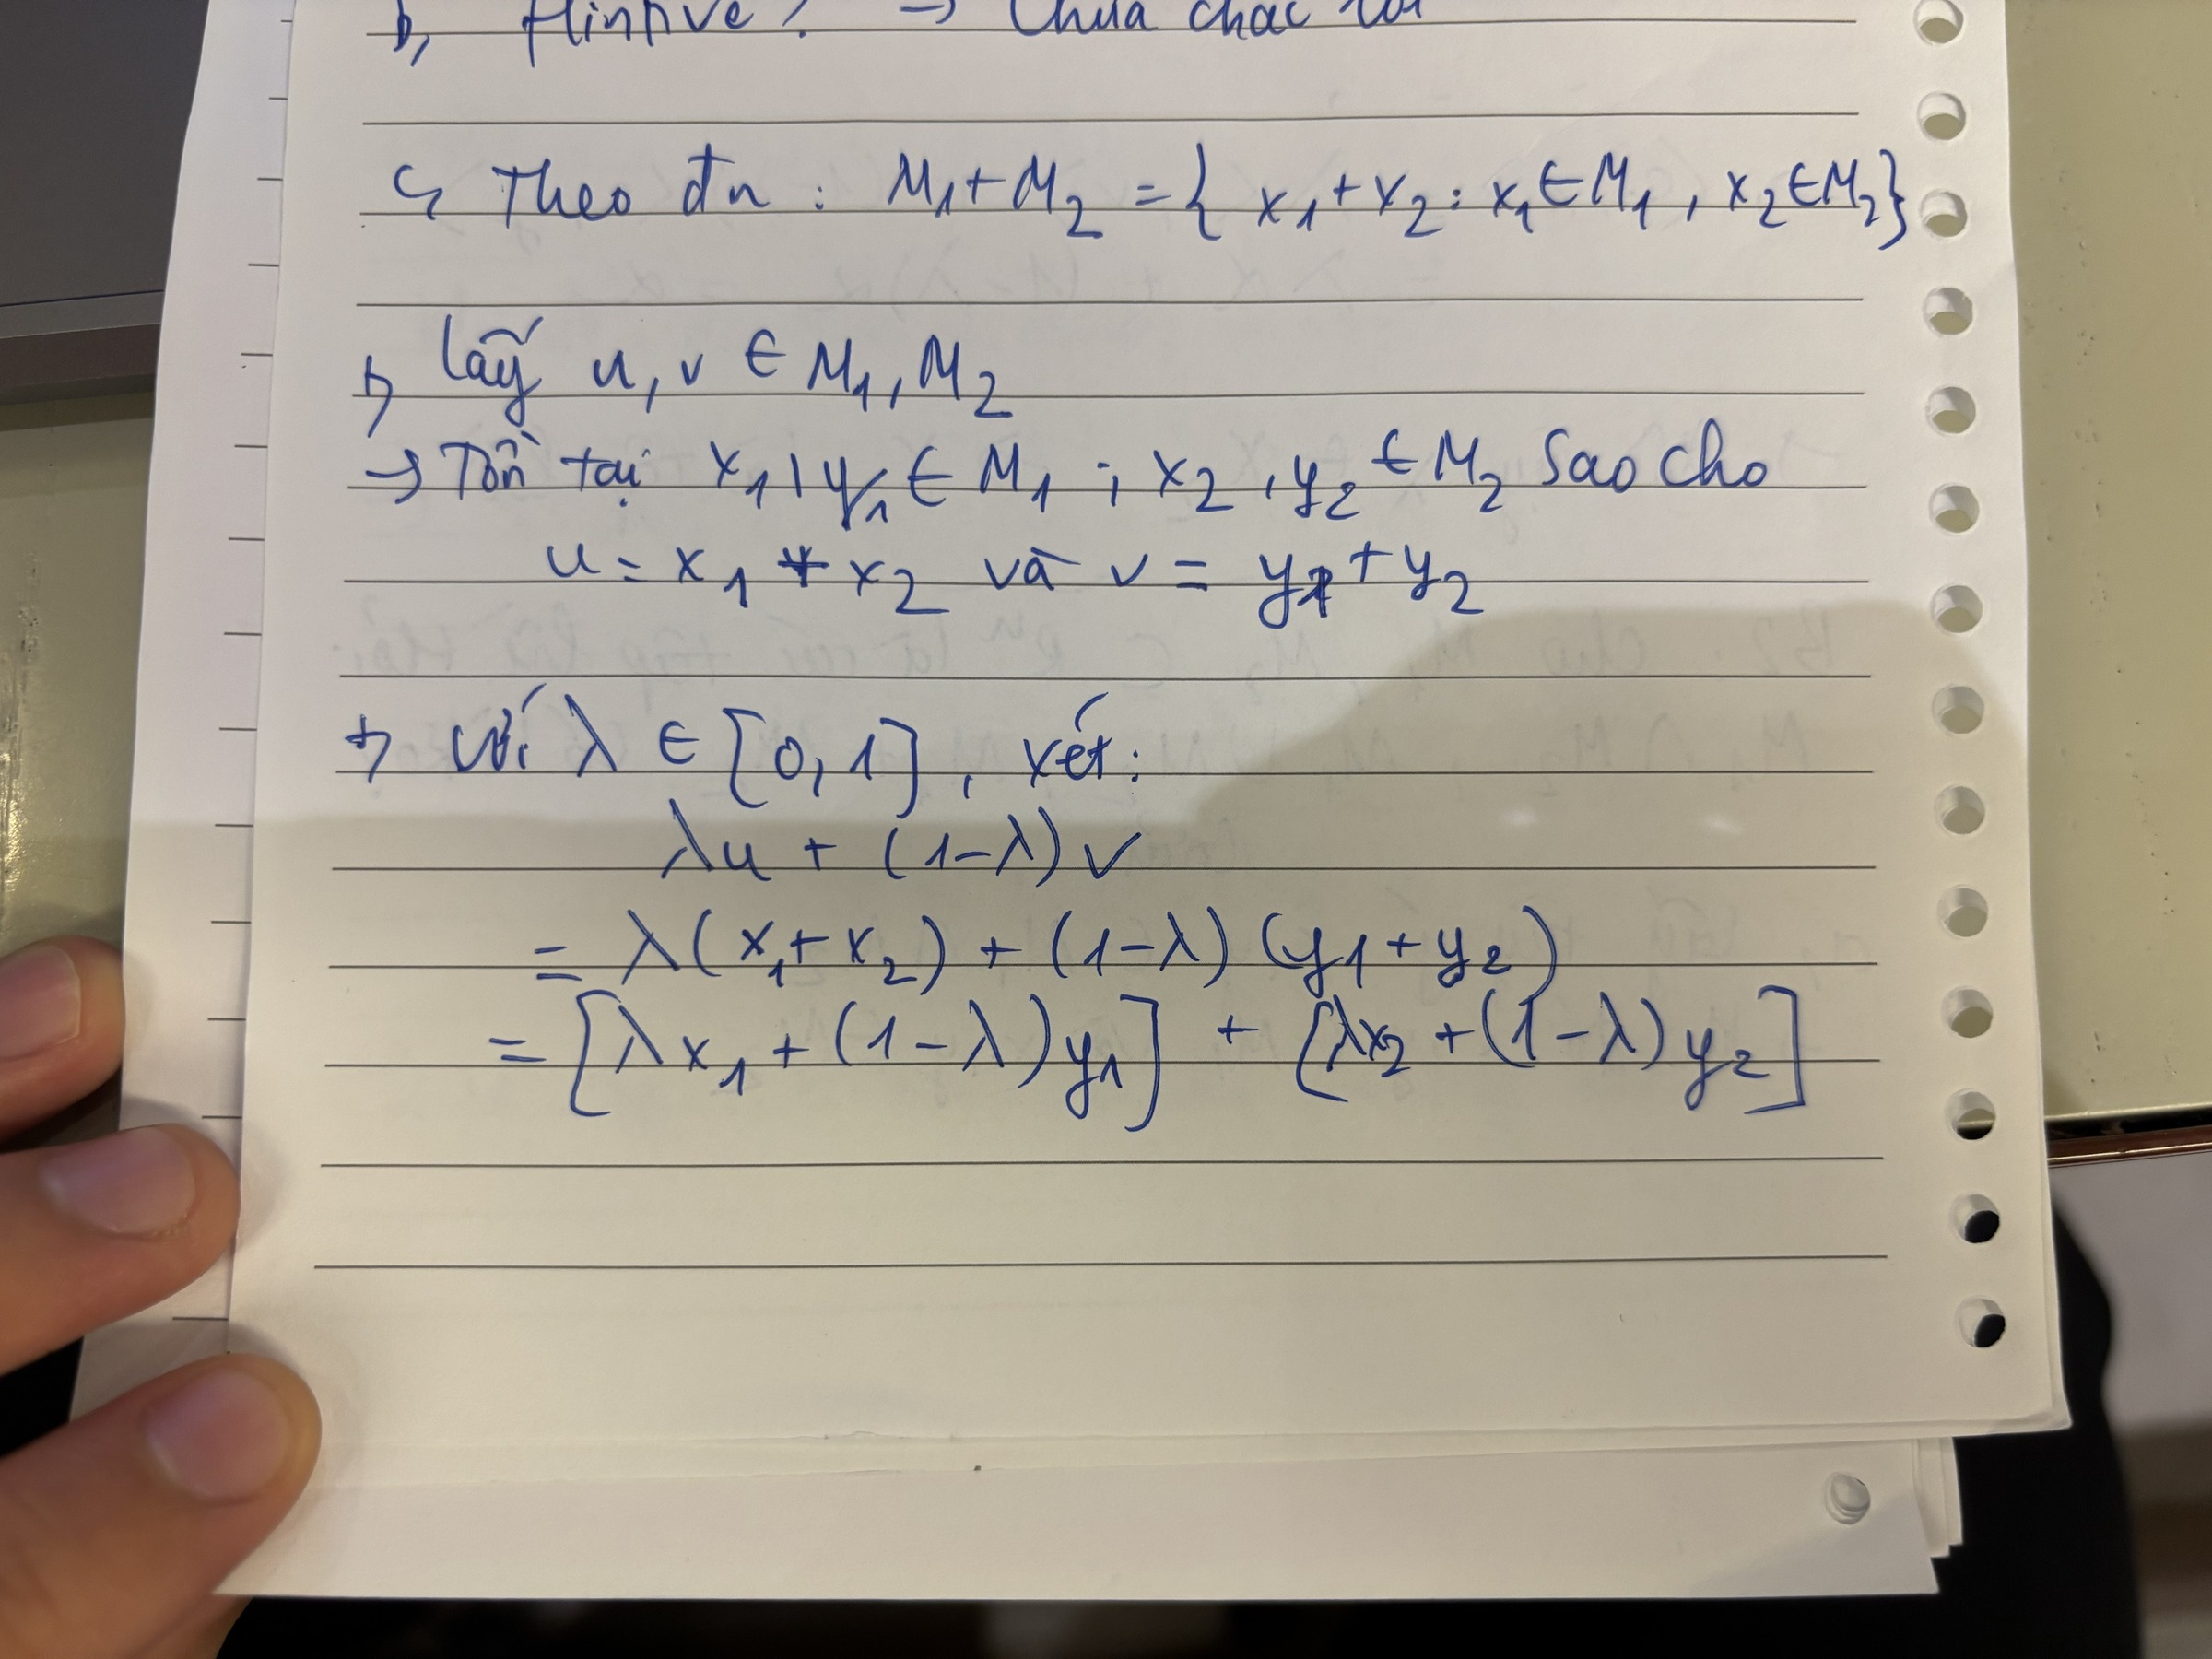
\includegraphics[width=.98\textwidth,height=.82\textheight,keepaspectratio]{bai_lam_them_1_assets/page-011.jpg}\end{center}
\clearpage
\phantomsection\label{src:012}
\noindent\textbf{Ảnh nguồn 012}\par\medskip
\begin{center}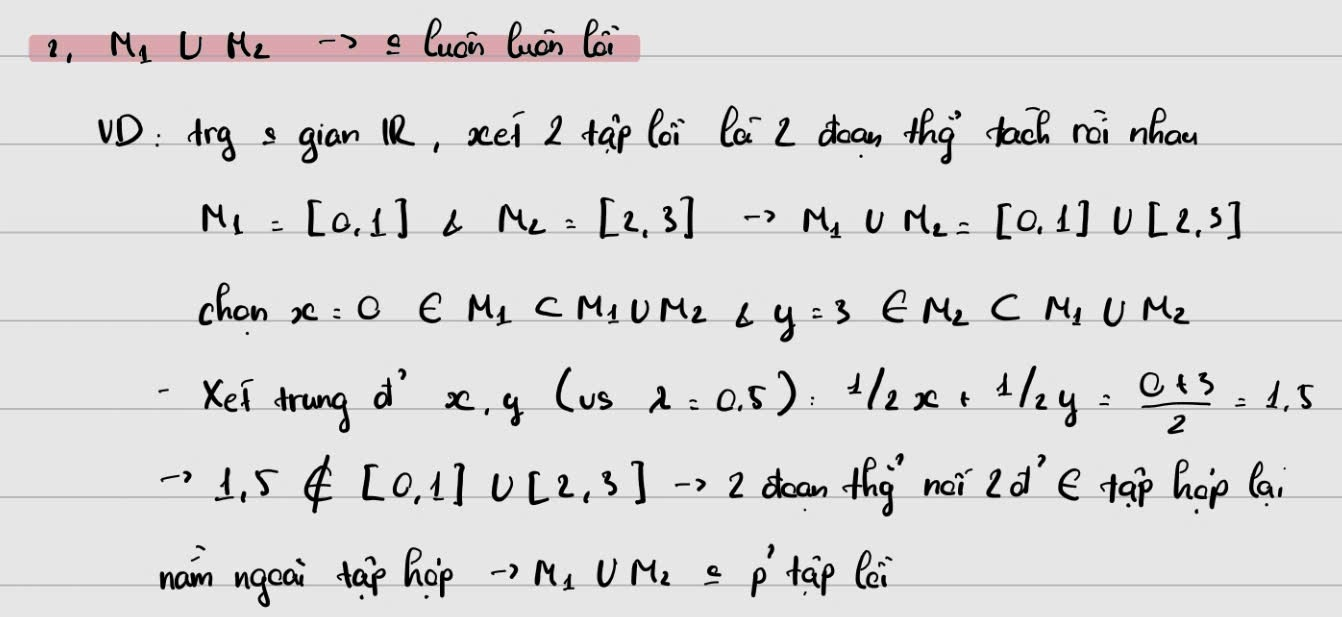
\includegraphics[width=.98\textwidth,height=.82\textheight,keepaspectratio]{bai_lam_them_1_assets/page-012.jpg}\end{center}
\clearpage
\phantomsection\label{src:013}
\noindent\textbf{Ảnh nguồn 013}\par\medskip
\begin{center}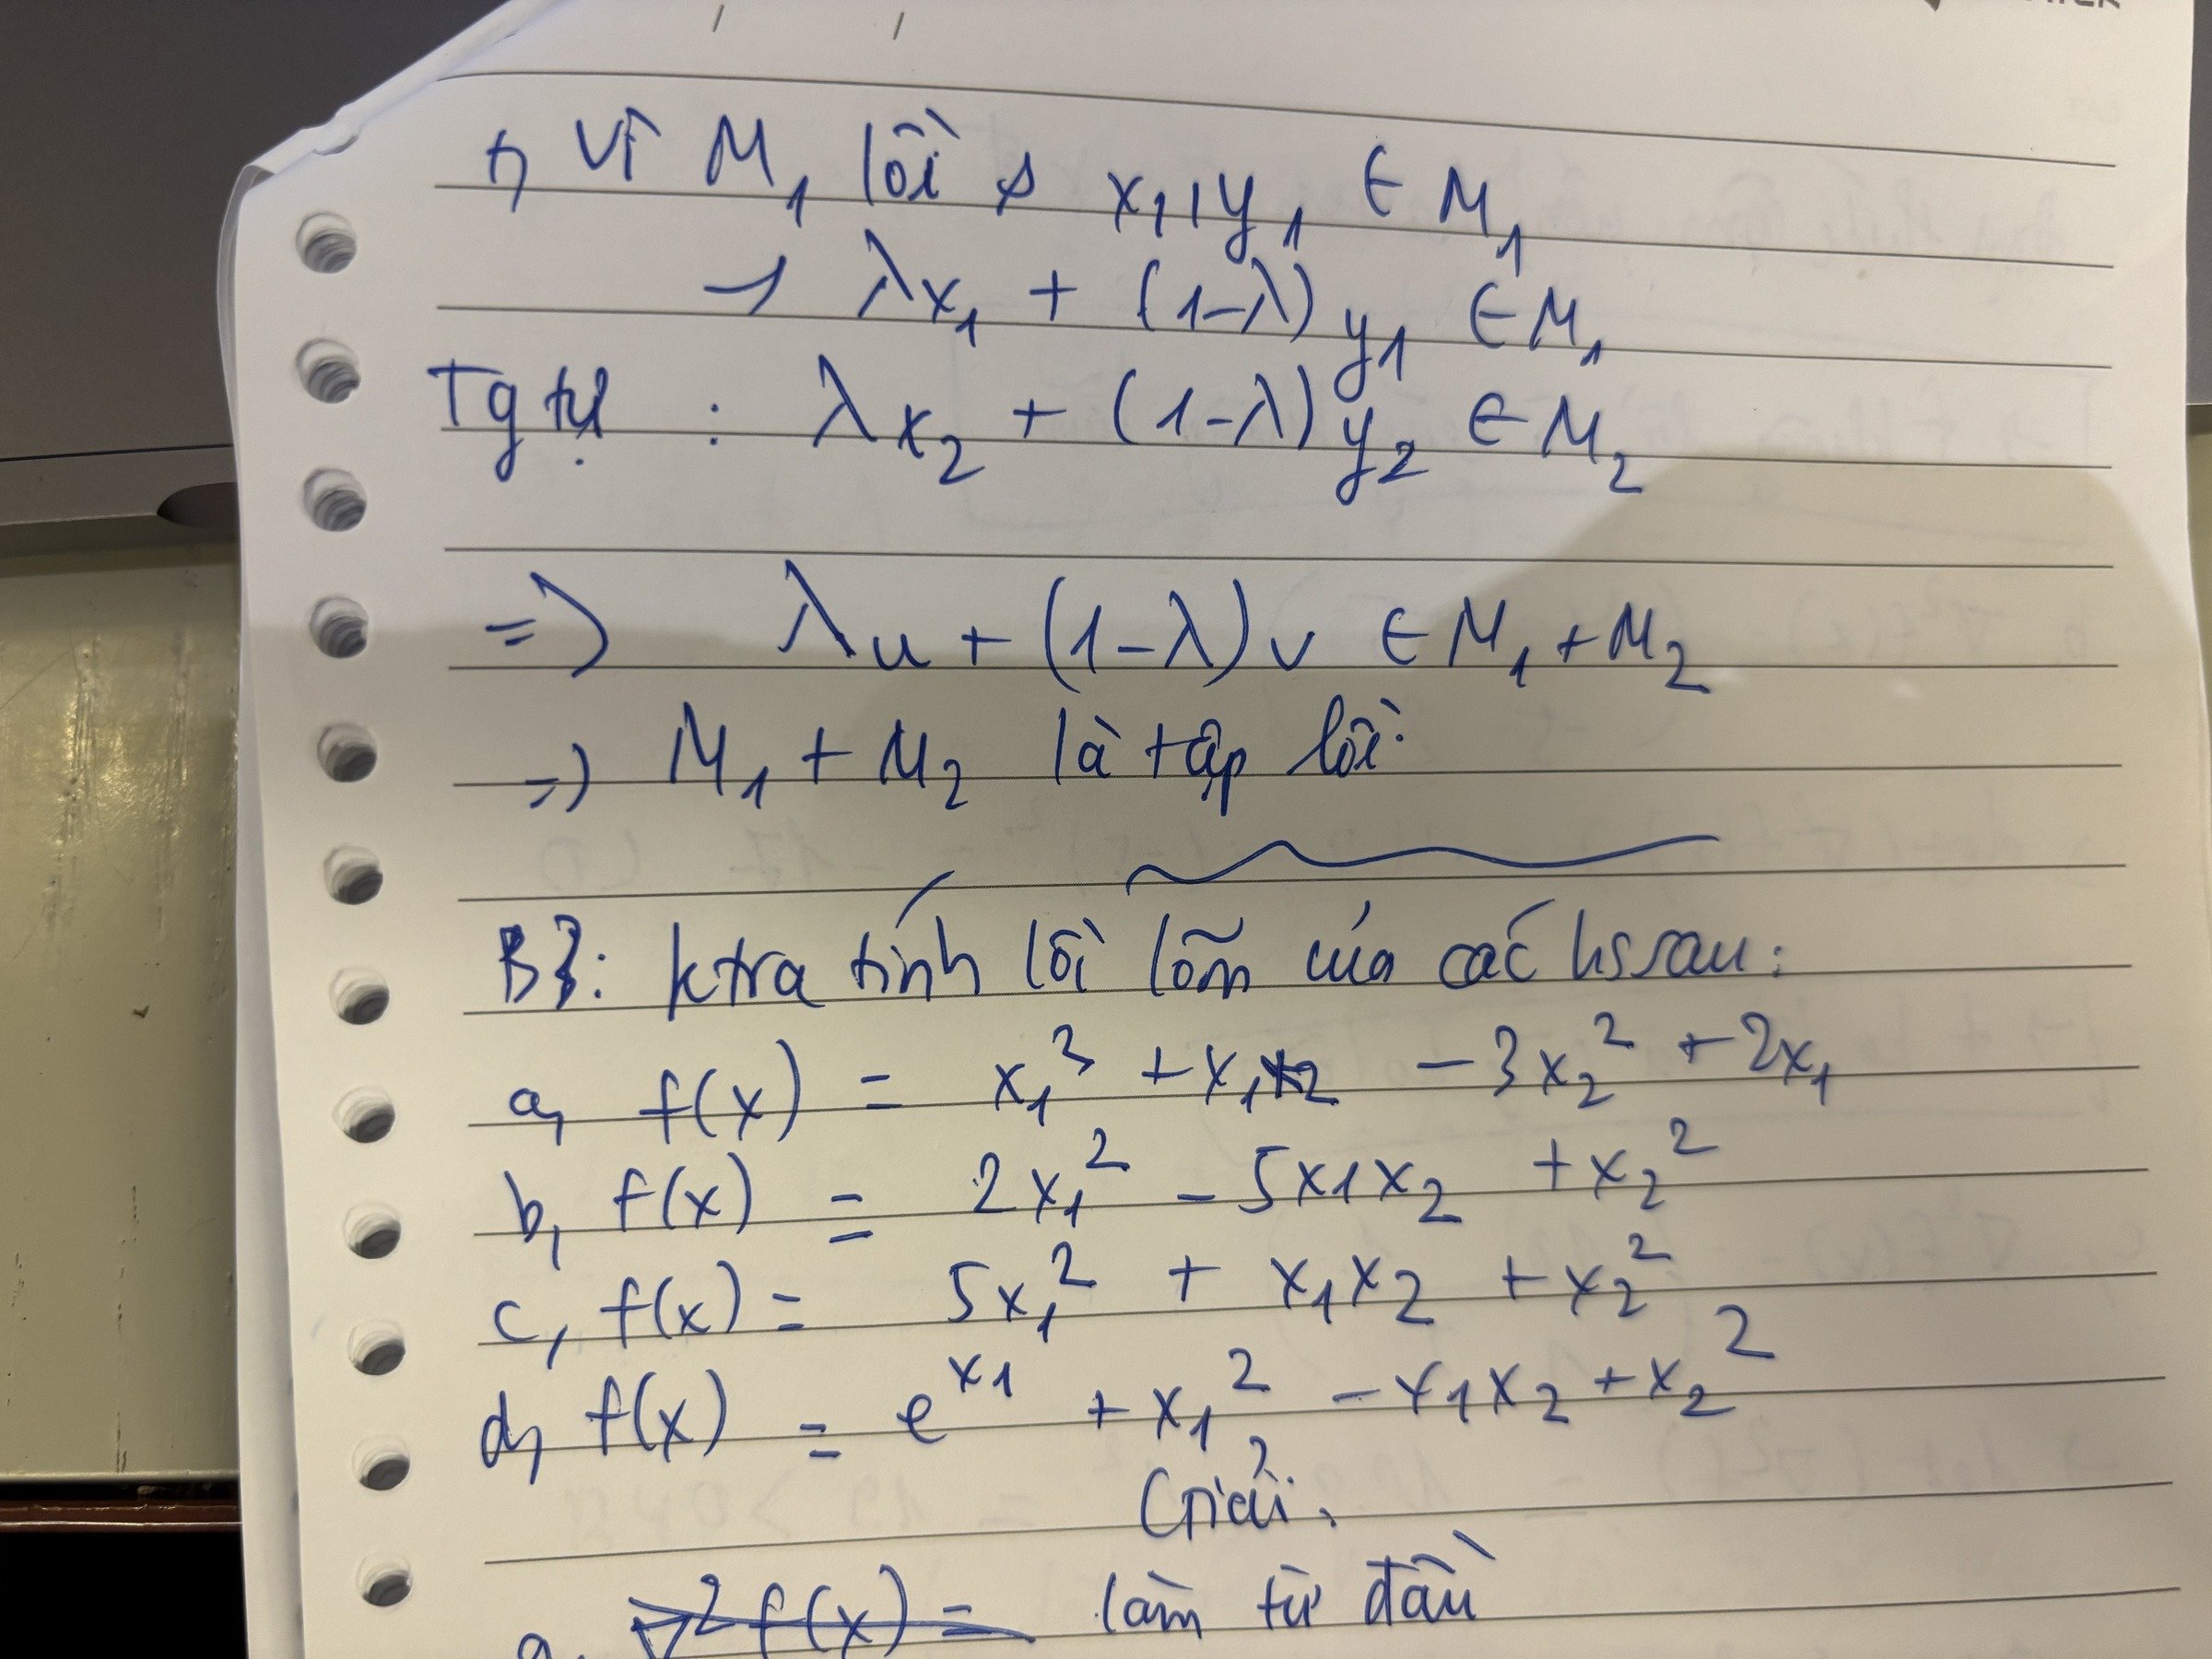
\includegraphics[width=.98\textwidth,height=.82\textheight,keepaspectratio]{bai_lam_them_1_assets/page-013.jpg}\end{center}
\clearpage
\phantomsection\label{src:014}
\noindent\textbf{Ảnh nguồn 014}\par\medskip
\begin{center}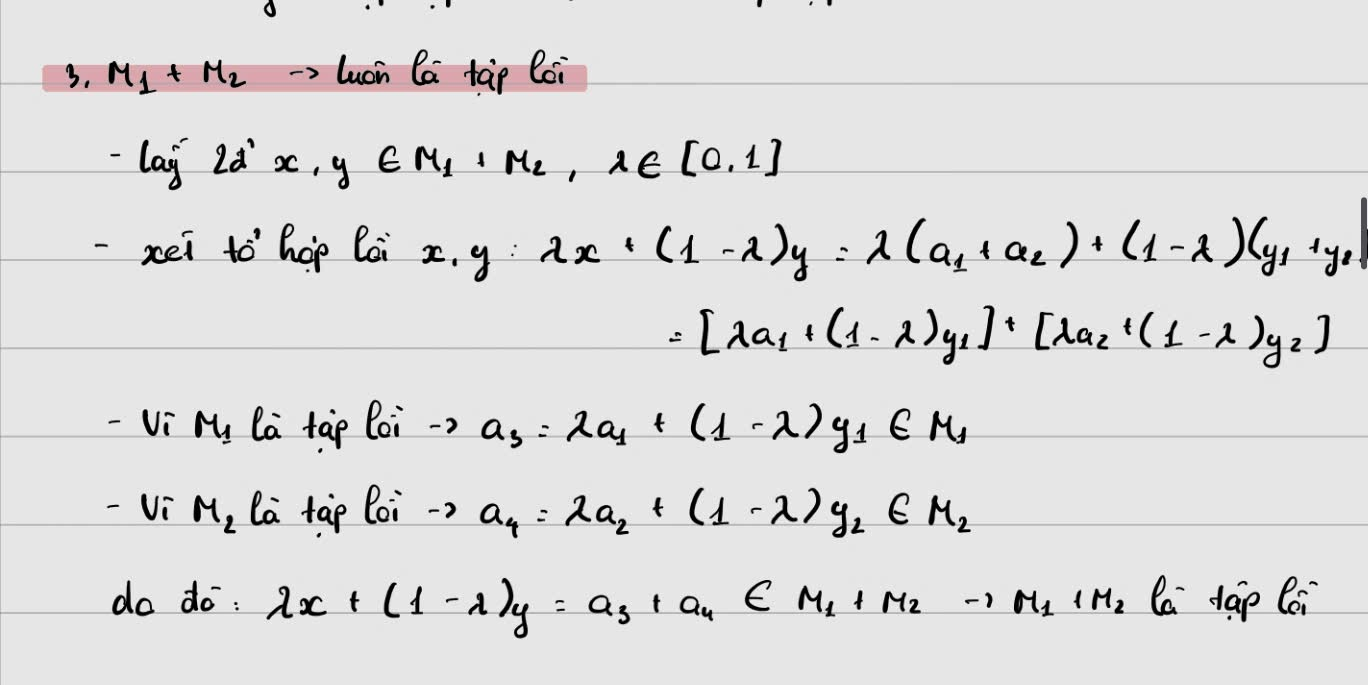
\includegraphics[width=.98\textwidth,height=.82\textheight,keepaspectratio]{bai_lam_them_1_assets/page-014.jpg}\end{center}
\clearpage
\phantomsection\label{src:015}
\noindent\textbf{Ảnh nguồn 015}\par\medskip
\begin{center}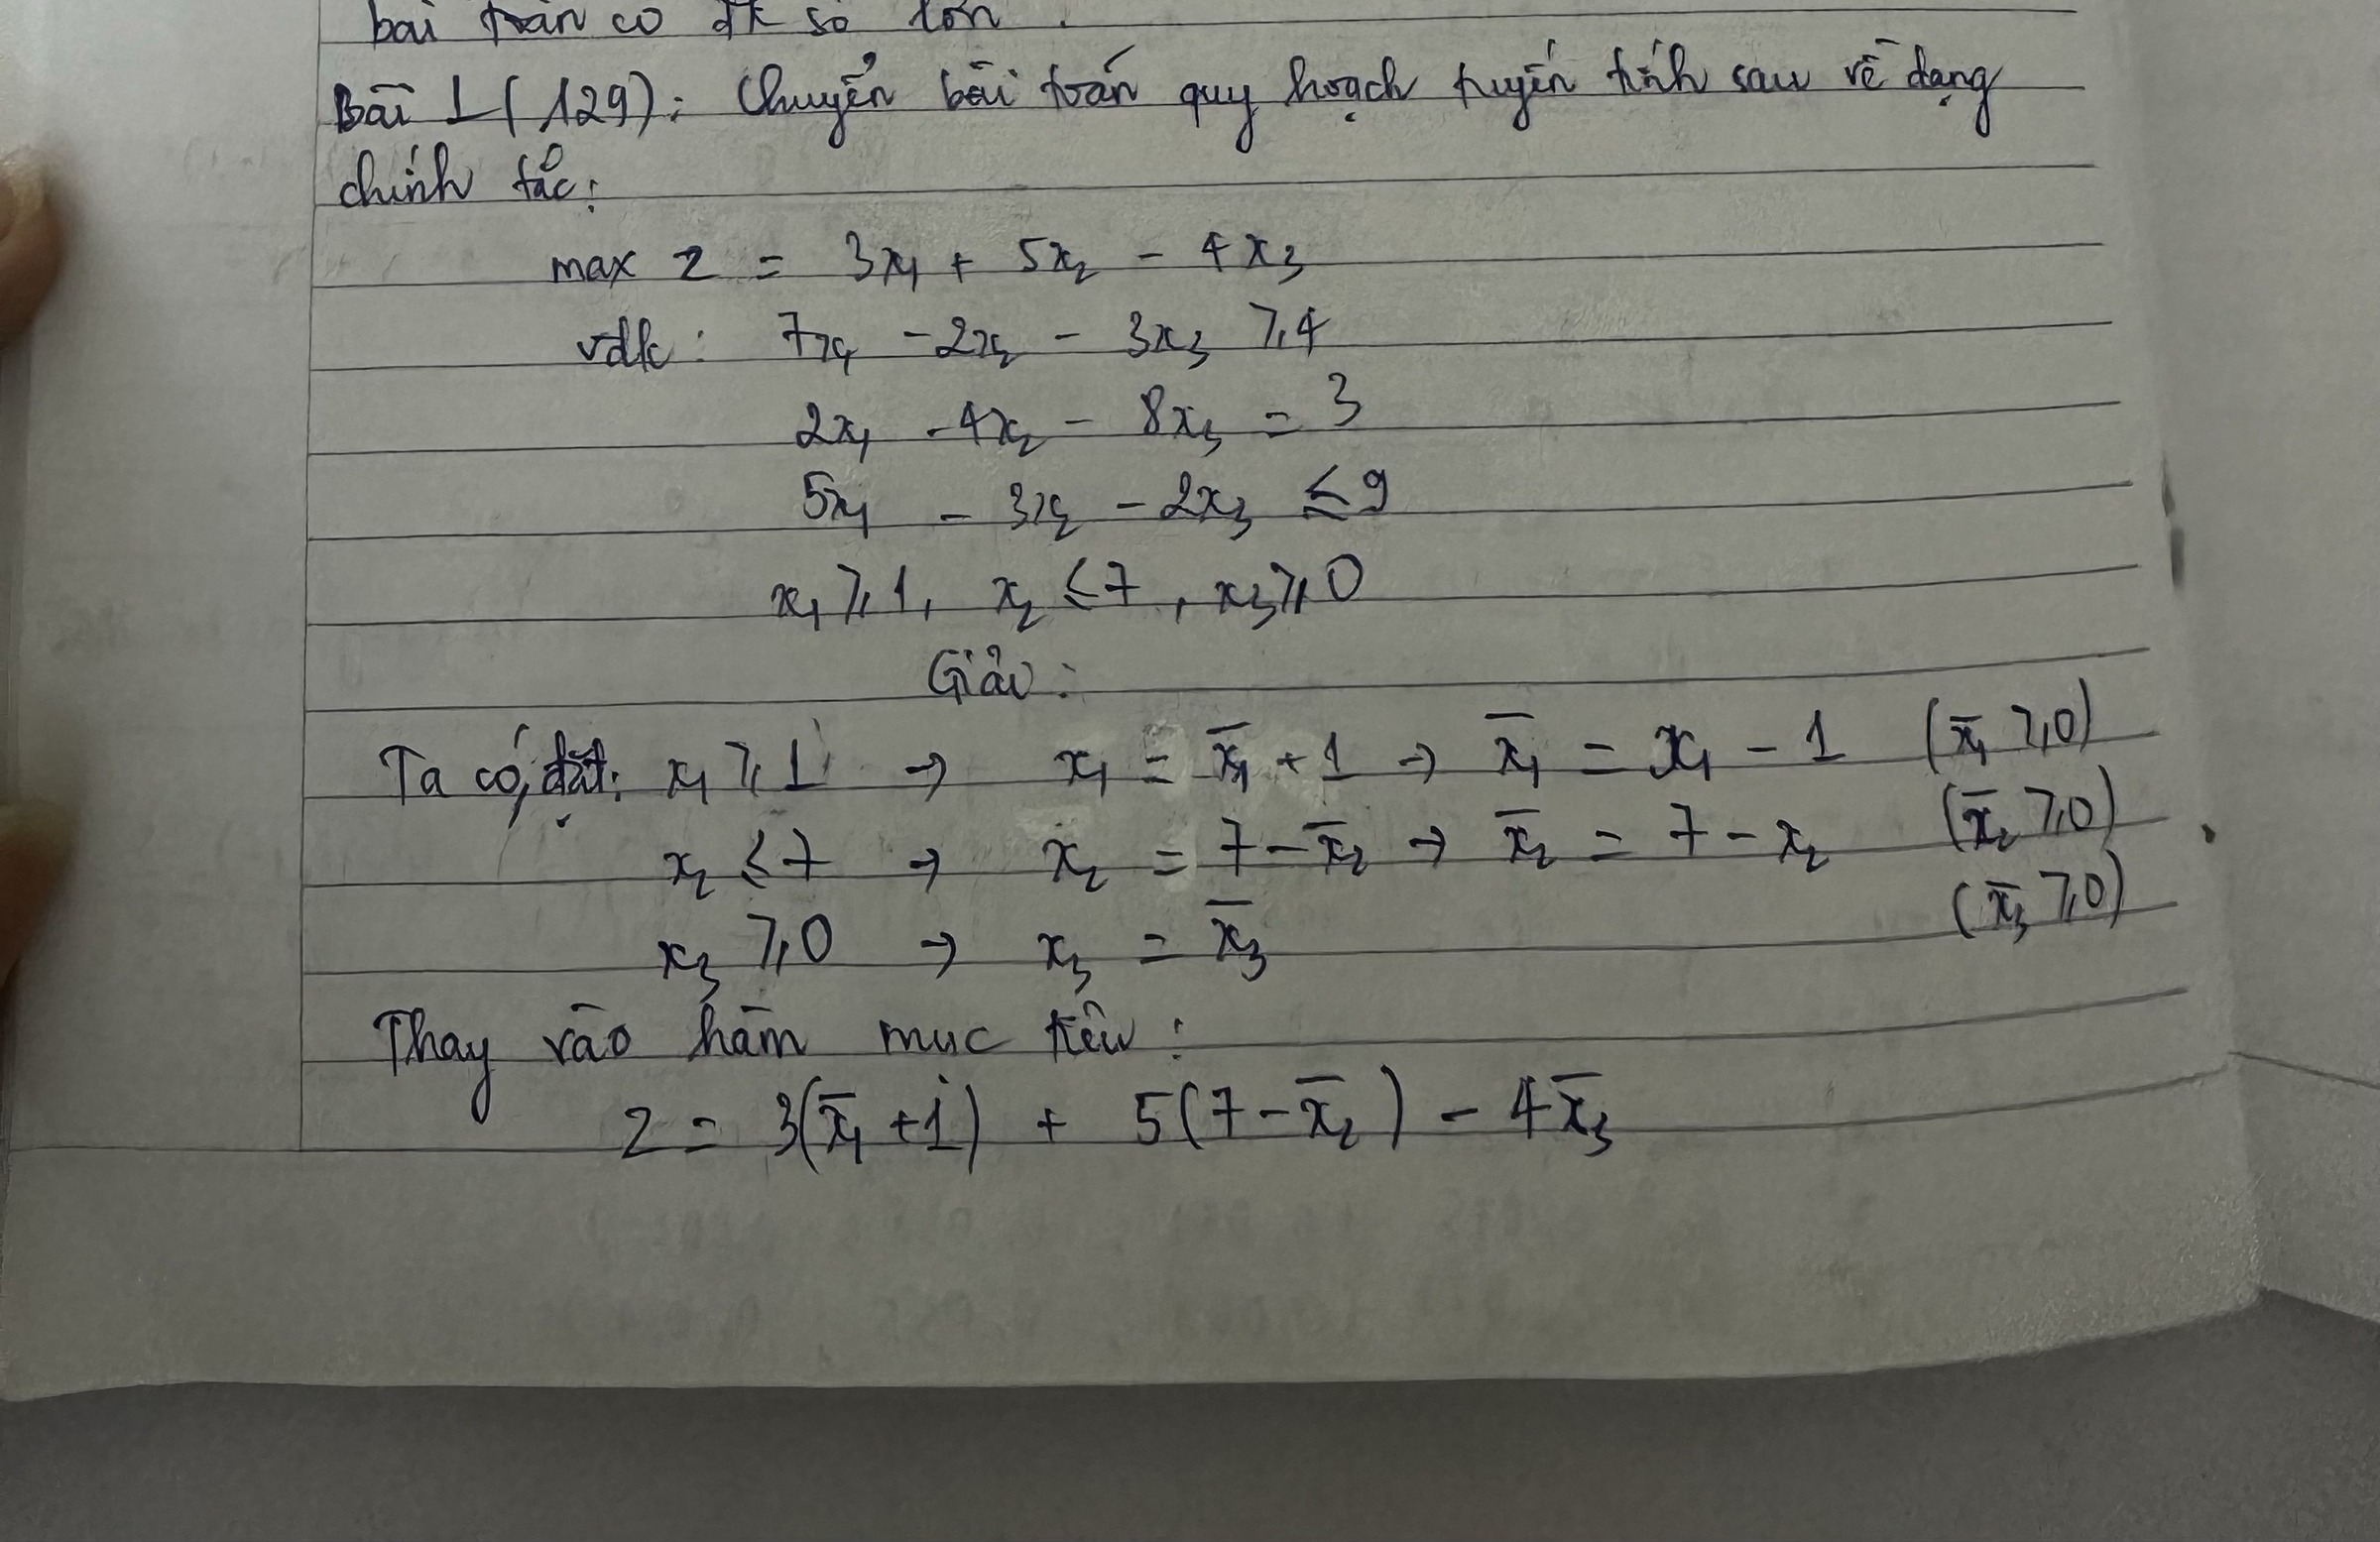
\includegraphics[width=.98\textwidth,height=.82\textheight,keepaspectratio]{bai_lam_them_1_assets/page-015.jpg}\end{center}
\clearpage
\phantomsection\label{src:016}
\noindent\textbf{Ảnh nguồn 016}\par\medskip
\begin{center}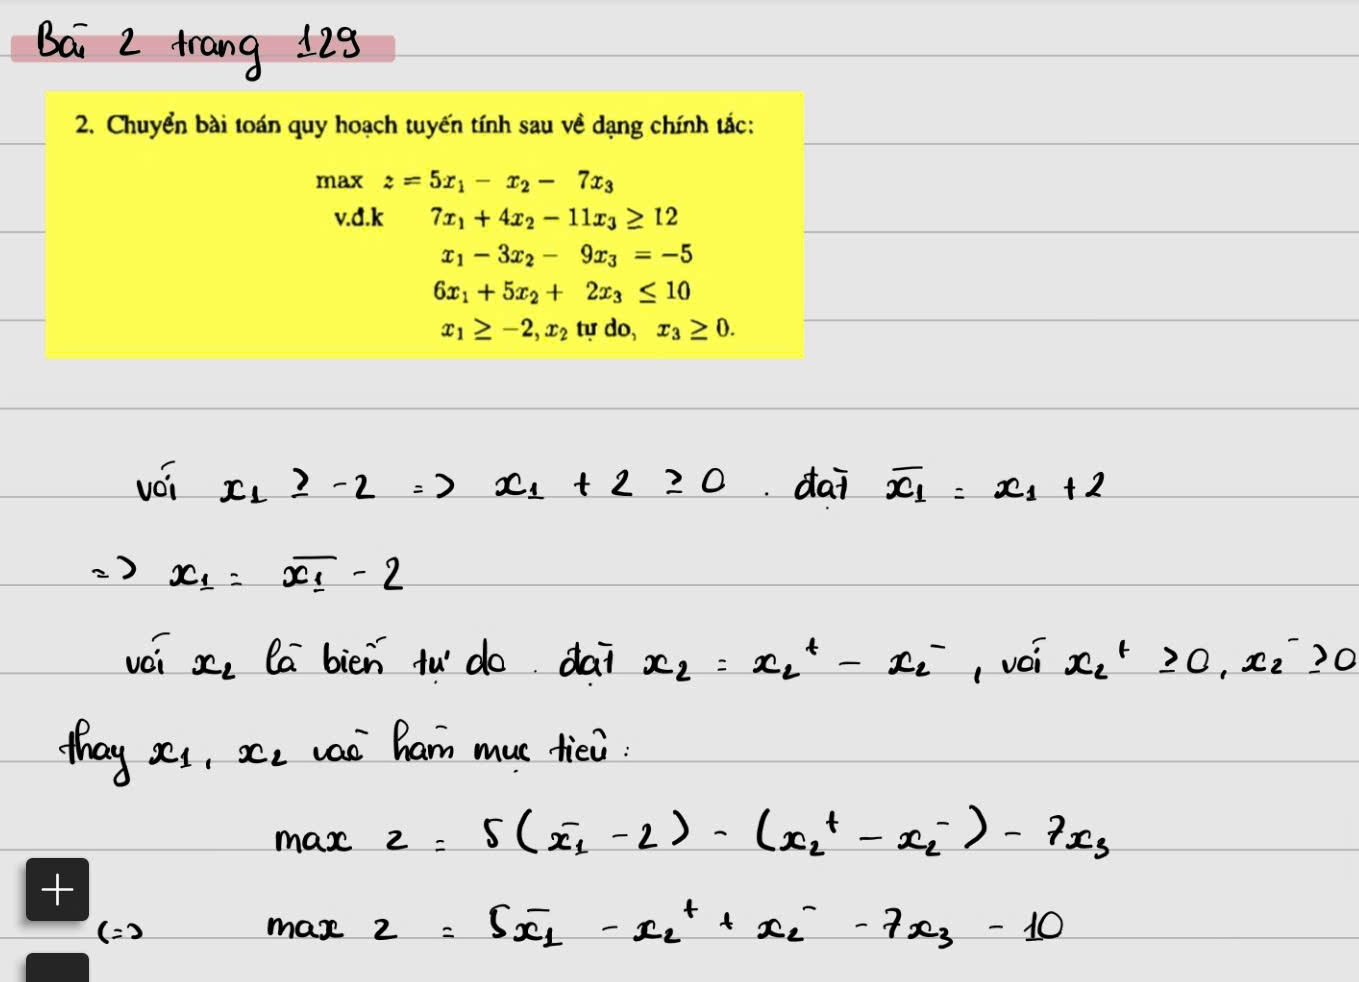
\includegraphics[width=.98\textwidth,height=.82\textheight,keepaspectratio]{bai_lam_them_1_assets/page-016.jpg}\end{center}
\clearpage
\phantomsection\label{src:017}
\noindent\textbf{Ảnh nguồn 017}\par\medskip
\begin{center}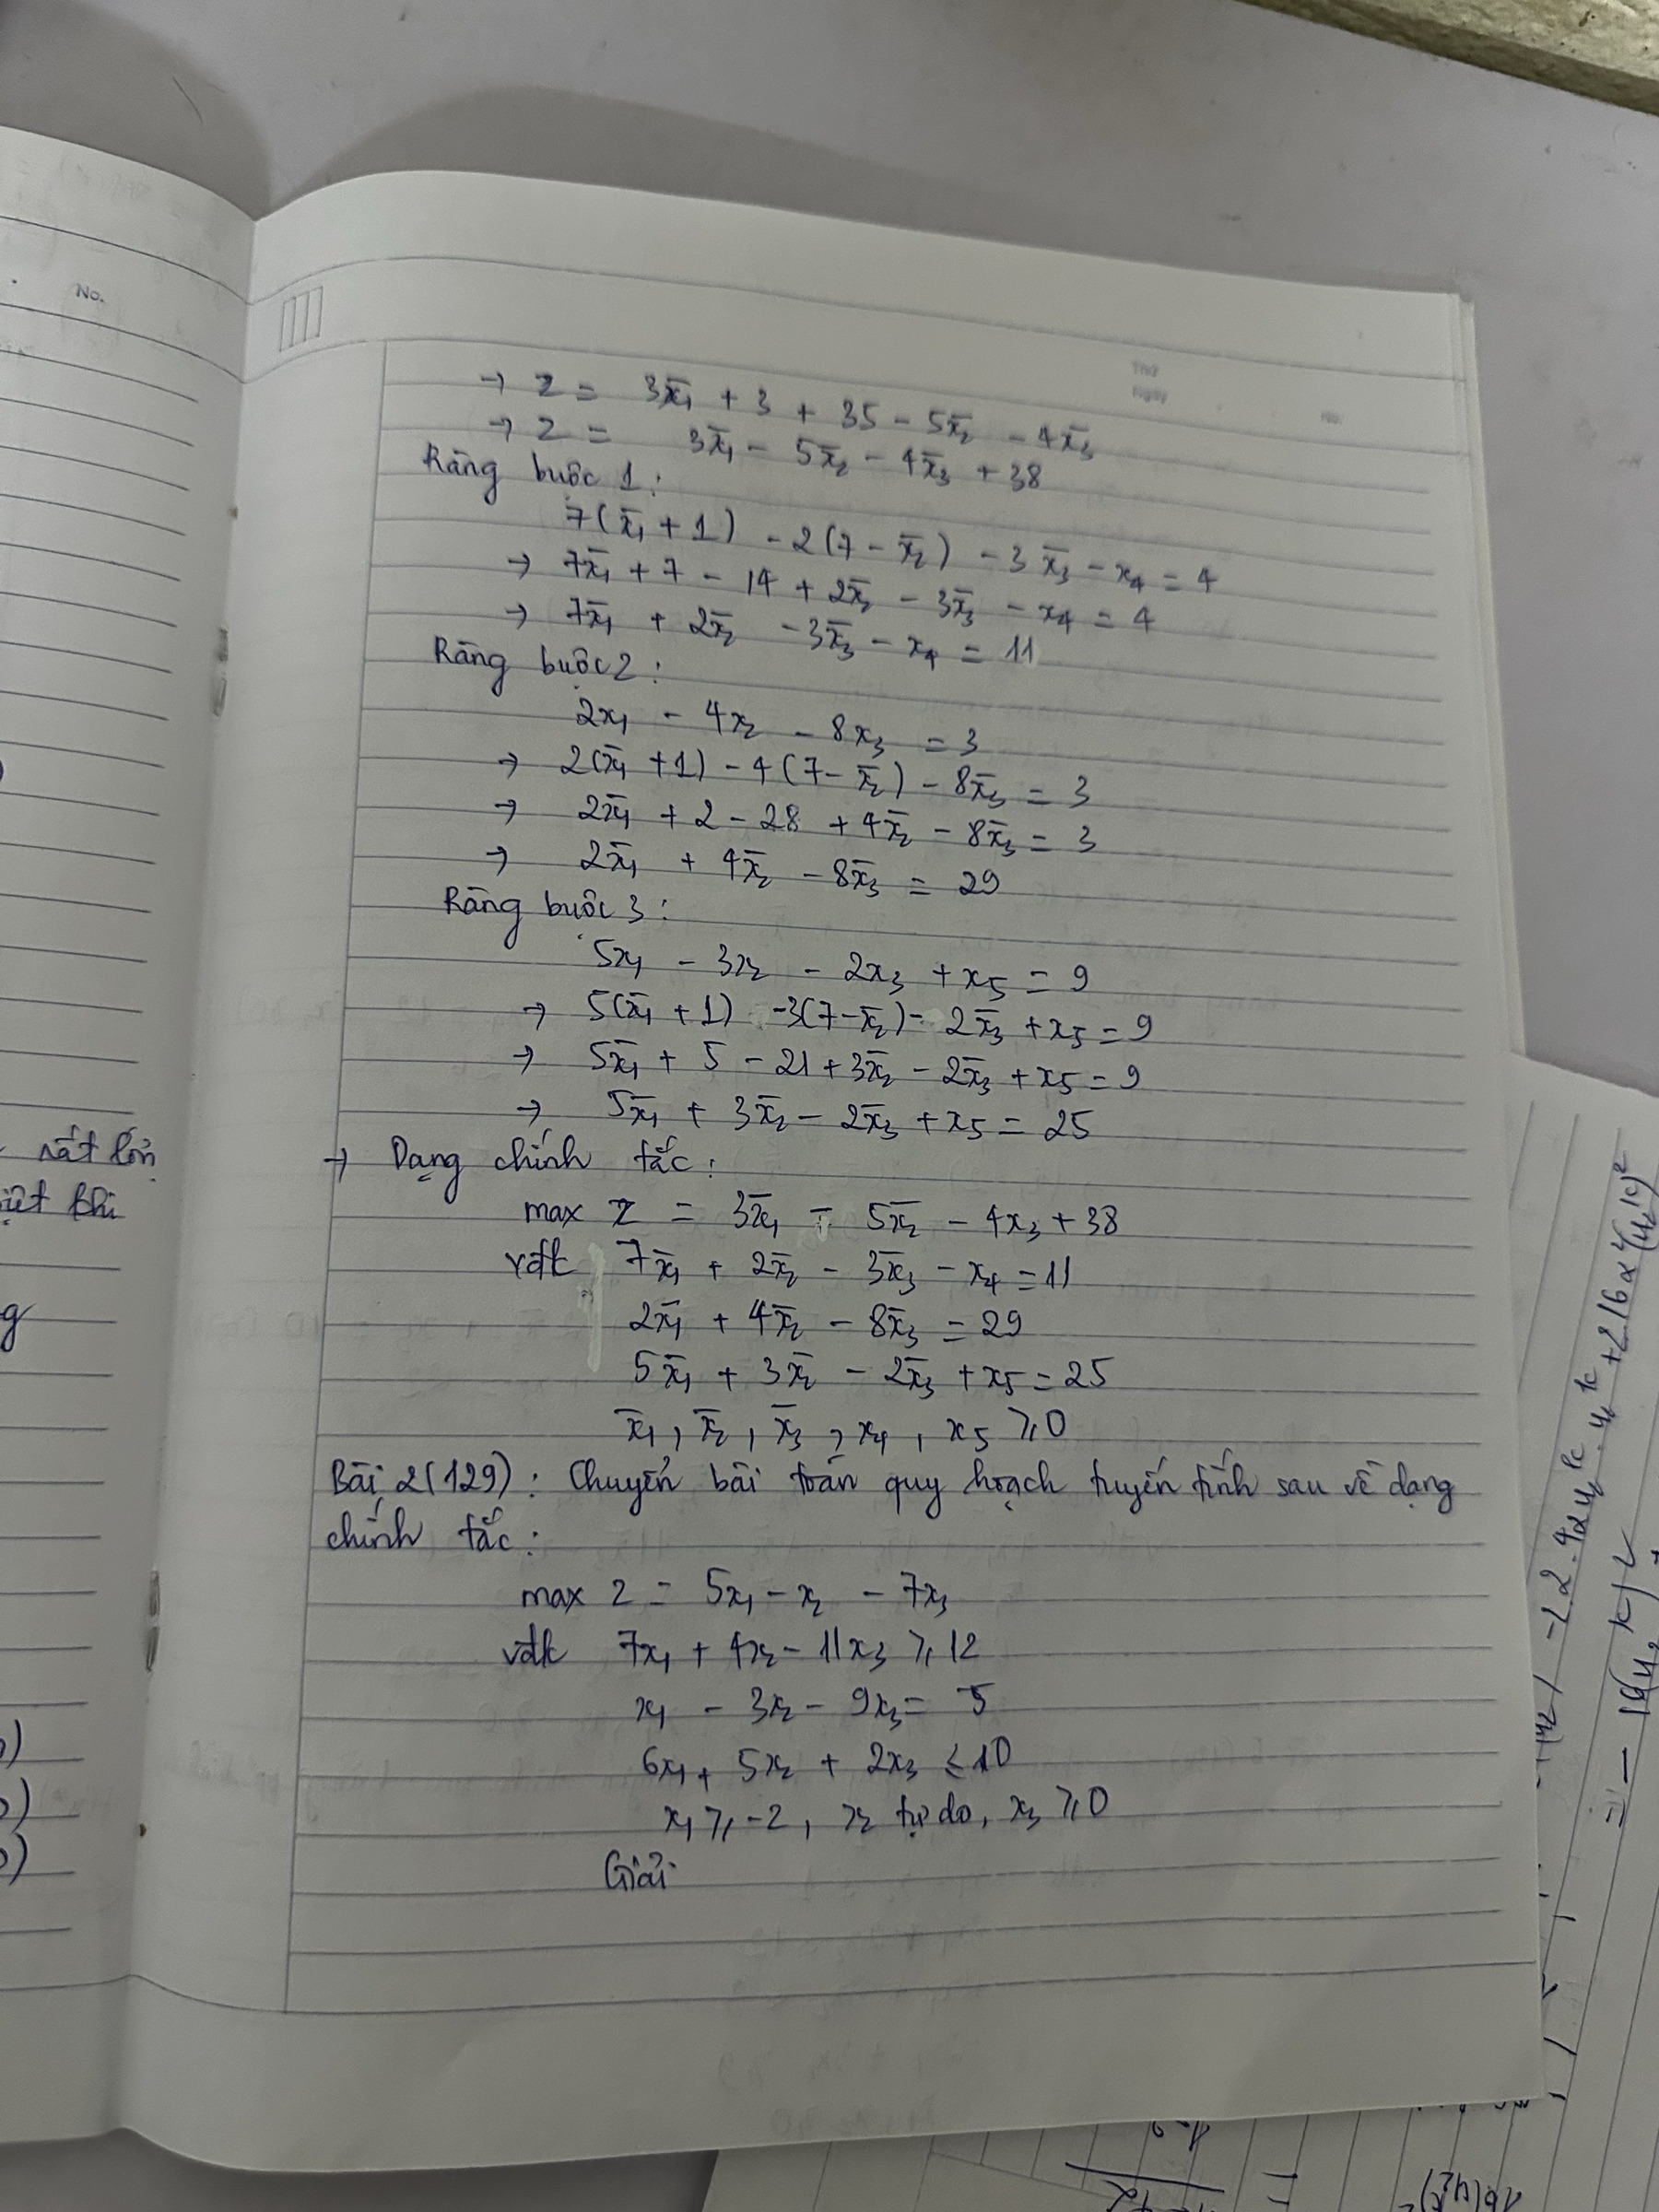
\includegraphics[width=.98\textwidth,height=.82\textheight,keepaspectratio]{bai_lam_them_1_assets/page-017.jpg}\end{center}
\clearpage
\phantomsection\label{src:018}
\noindent\textbf{Ảnh nguồn 018}\par\medskip
\begin{center}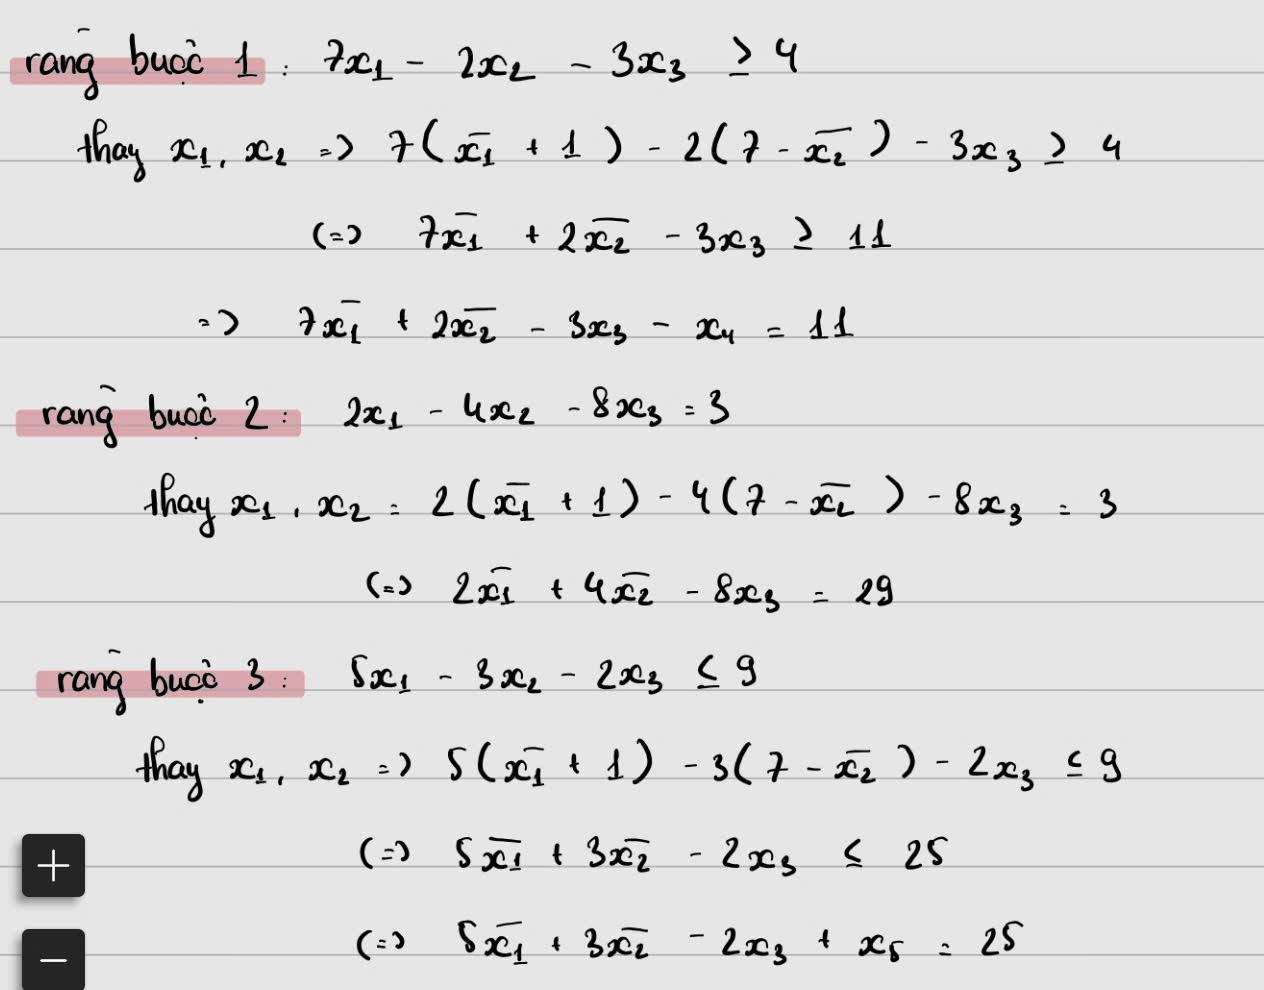
\includegraphics[width=.98\textwidth,height=.82\textheight,keepaspectratio]{bai_lam_them_1_assets/page-018.jpg}\end{center}
\clearpage
\phantomsection\label{src:019}
\noindent\textbf{Ảnh nguồn 019}\par\medskip
\begin{center}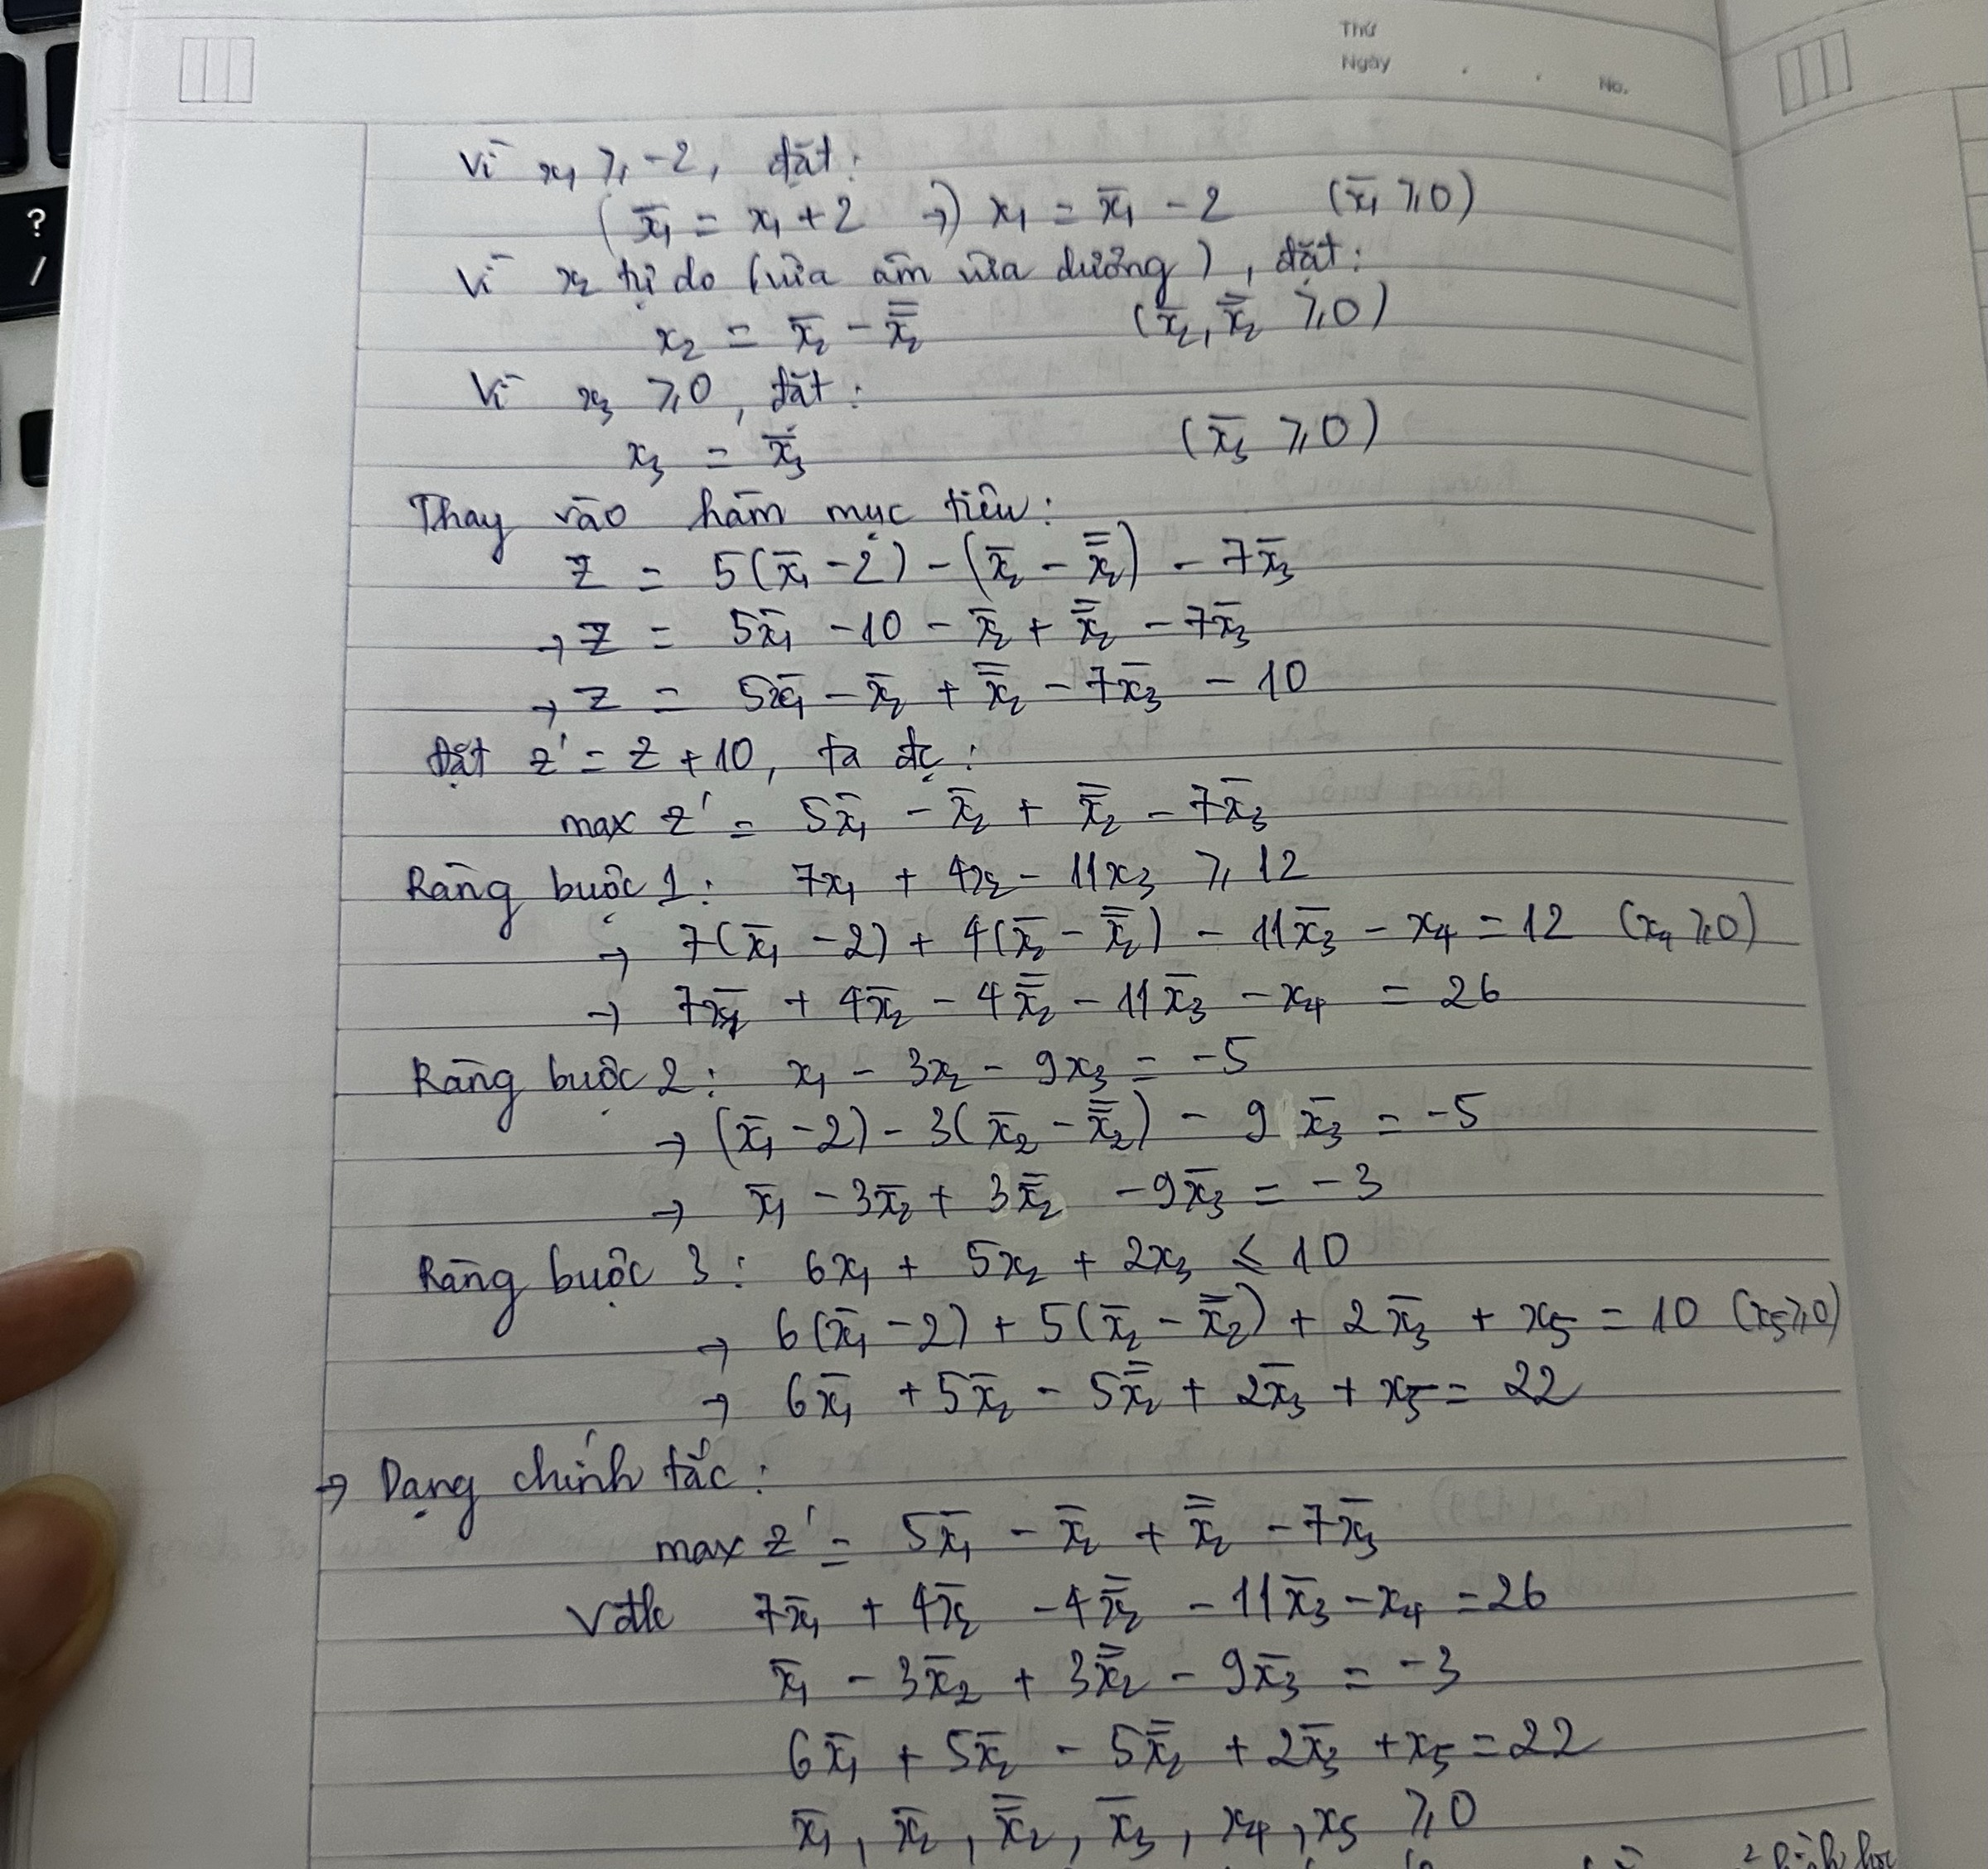
\includegraphics[width=.98\textwidth,height=.82\textheight,keepaspectratio]{bai_lam_them_1_assets/page-019.jpg}\end{center}
\clearpage
\phantomsection\label{src:020}
\noindent\textbf{Ảnh nguồn 020}\par\medskip
\begin{center}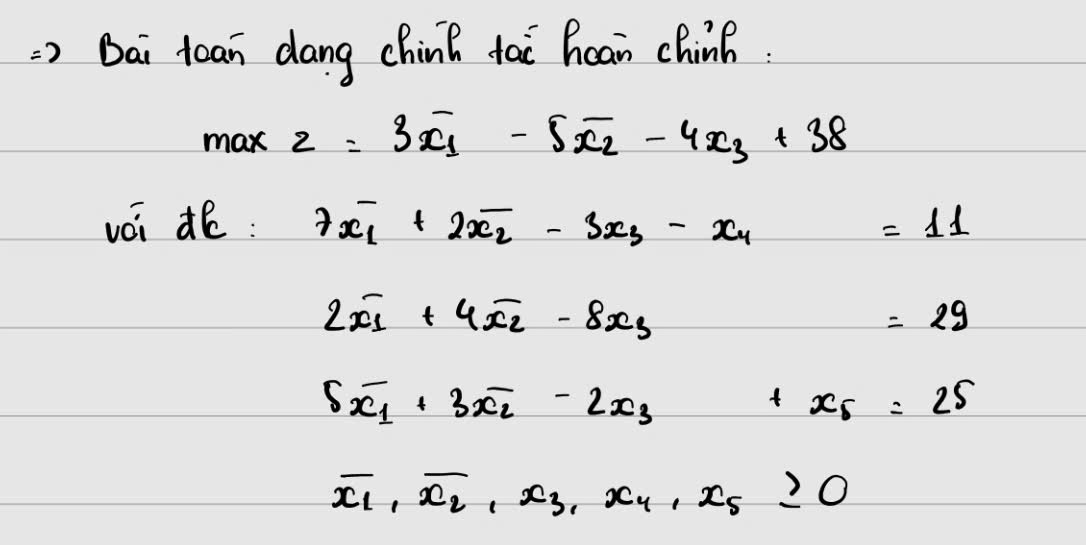
\includegraphics[width=.98\textwidth,height=.82\textheight,keepaspectratio]{bai_lam_them_1_assets/page-020.jpg}\end{center}
\clearpage
\phantomsection\label{src:021}
\noindent\textbf{Ảnh nguồn 021}\par\medskip
\begin{center}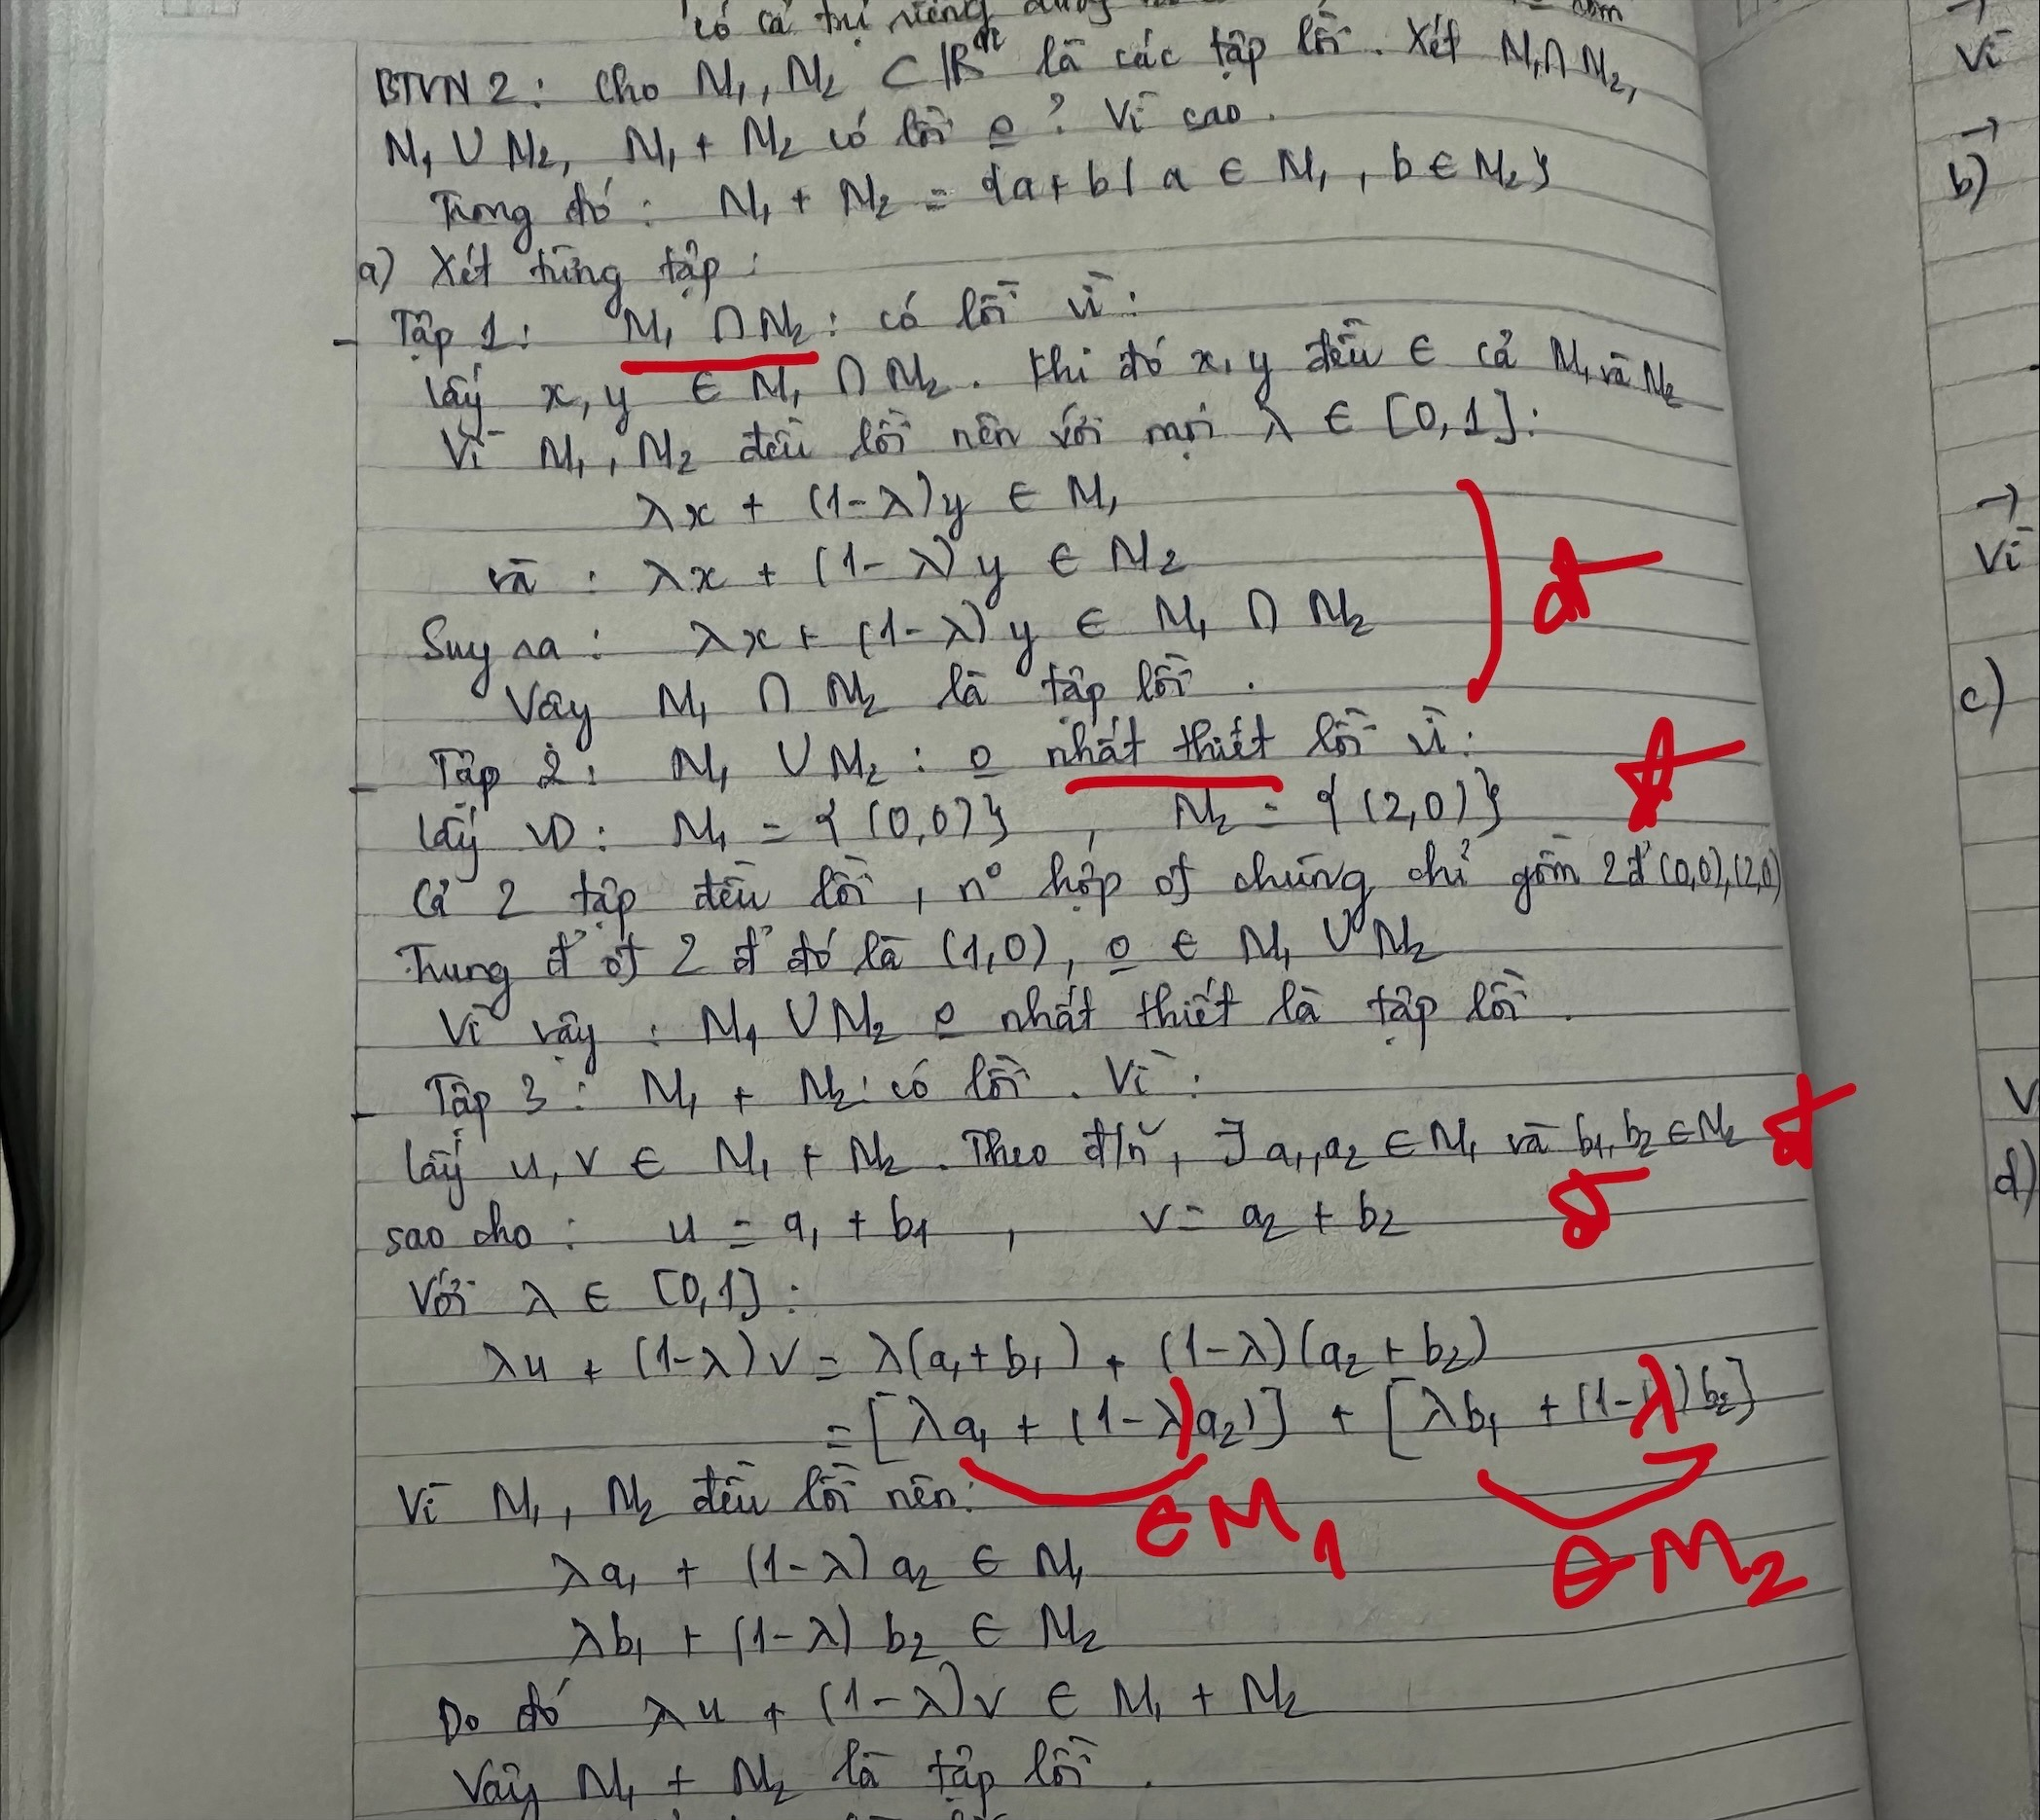
\includegraphics[width=.98\textwidth,height=.82\textheight,keepaspectratio]{bai_lam_them_1_assets/page-021.jpg}\end{center}
\clearpage
\phantomsection\label{src:022}
\noindent\textbf{Ảnh nguồn 022}\par\medskip
\begin{center}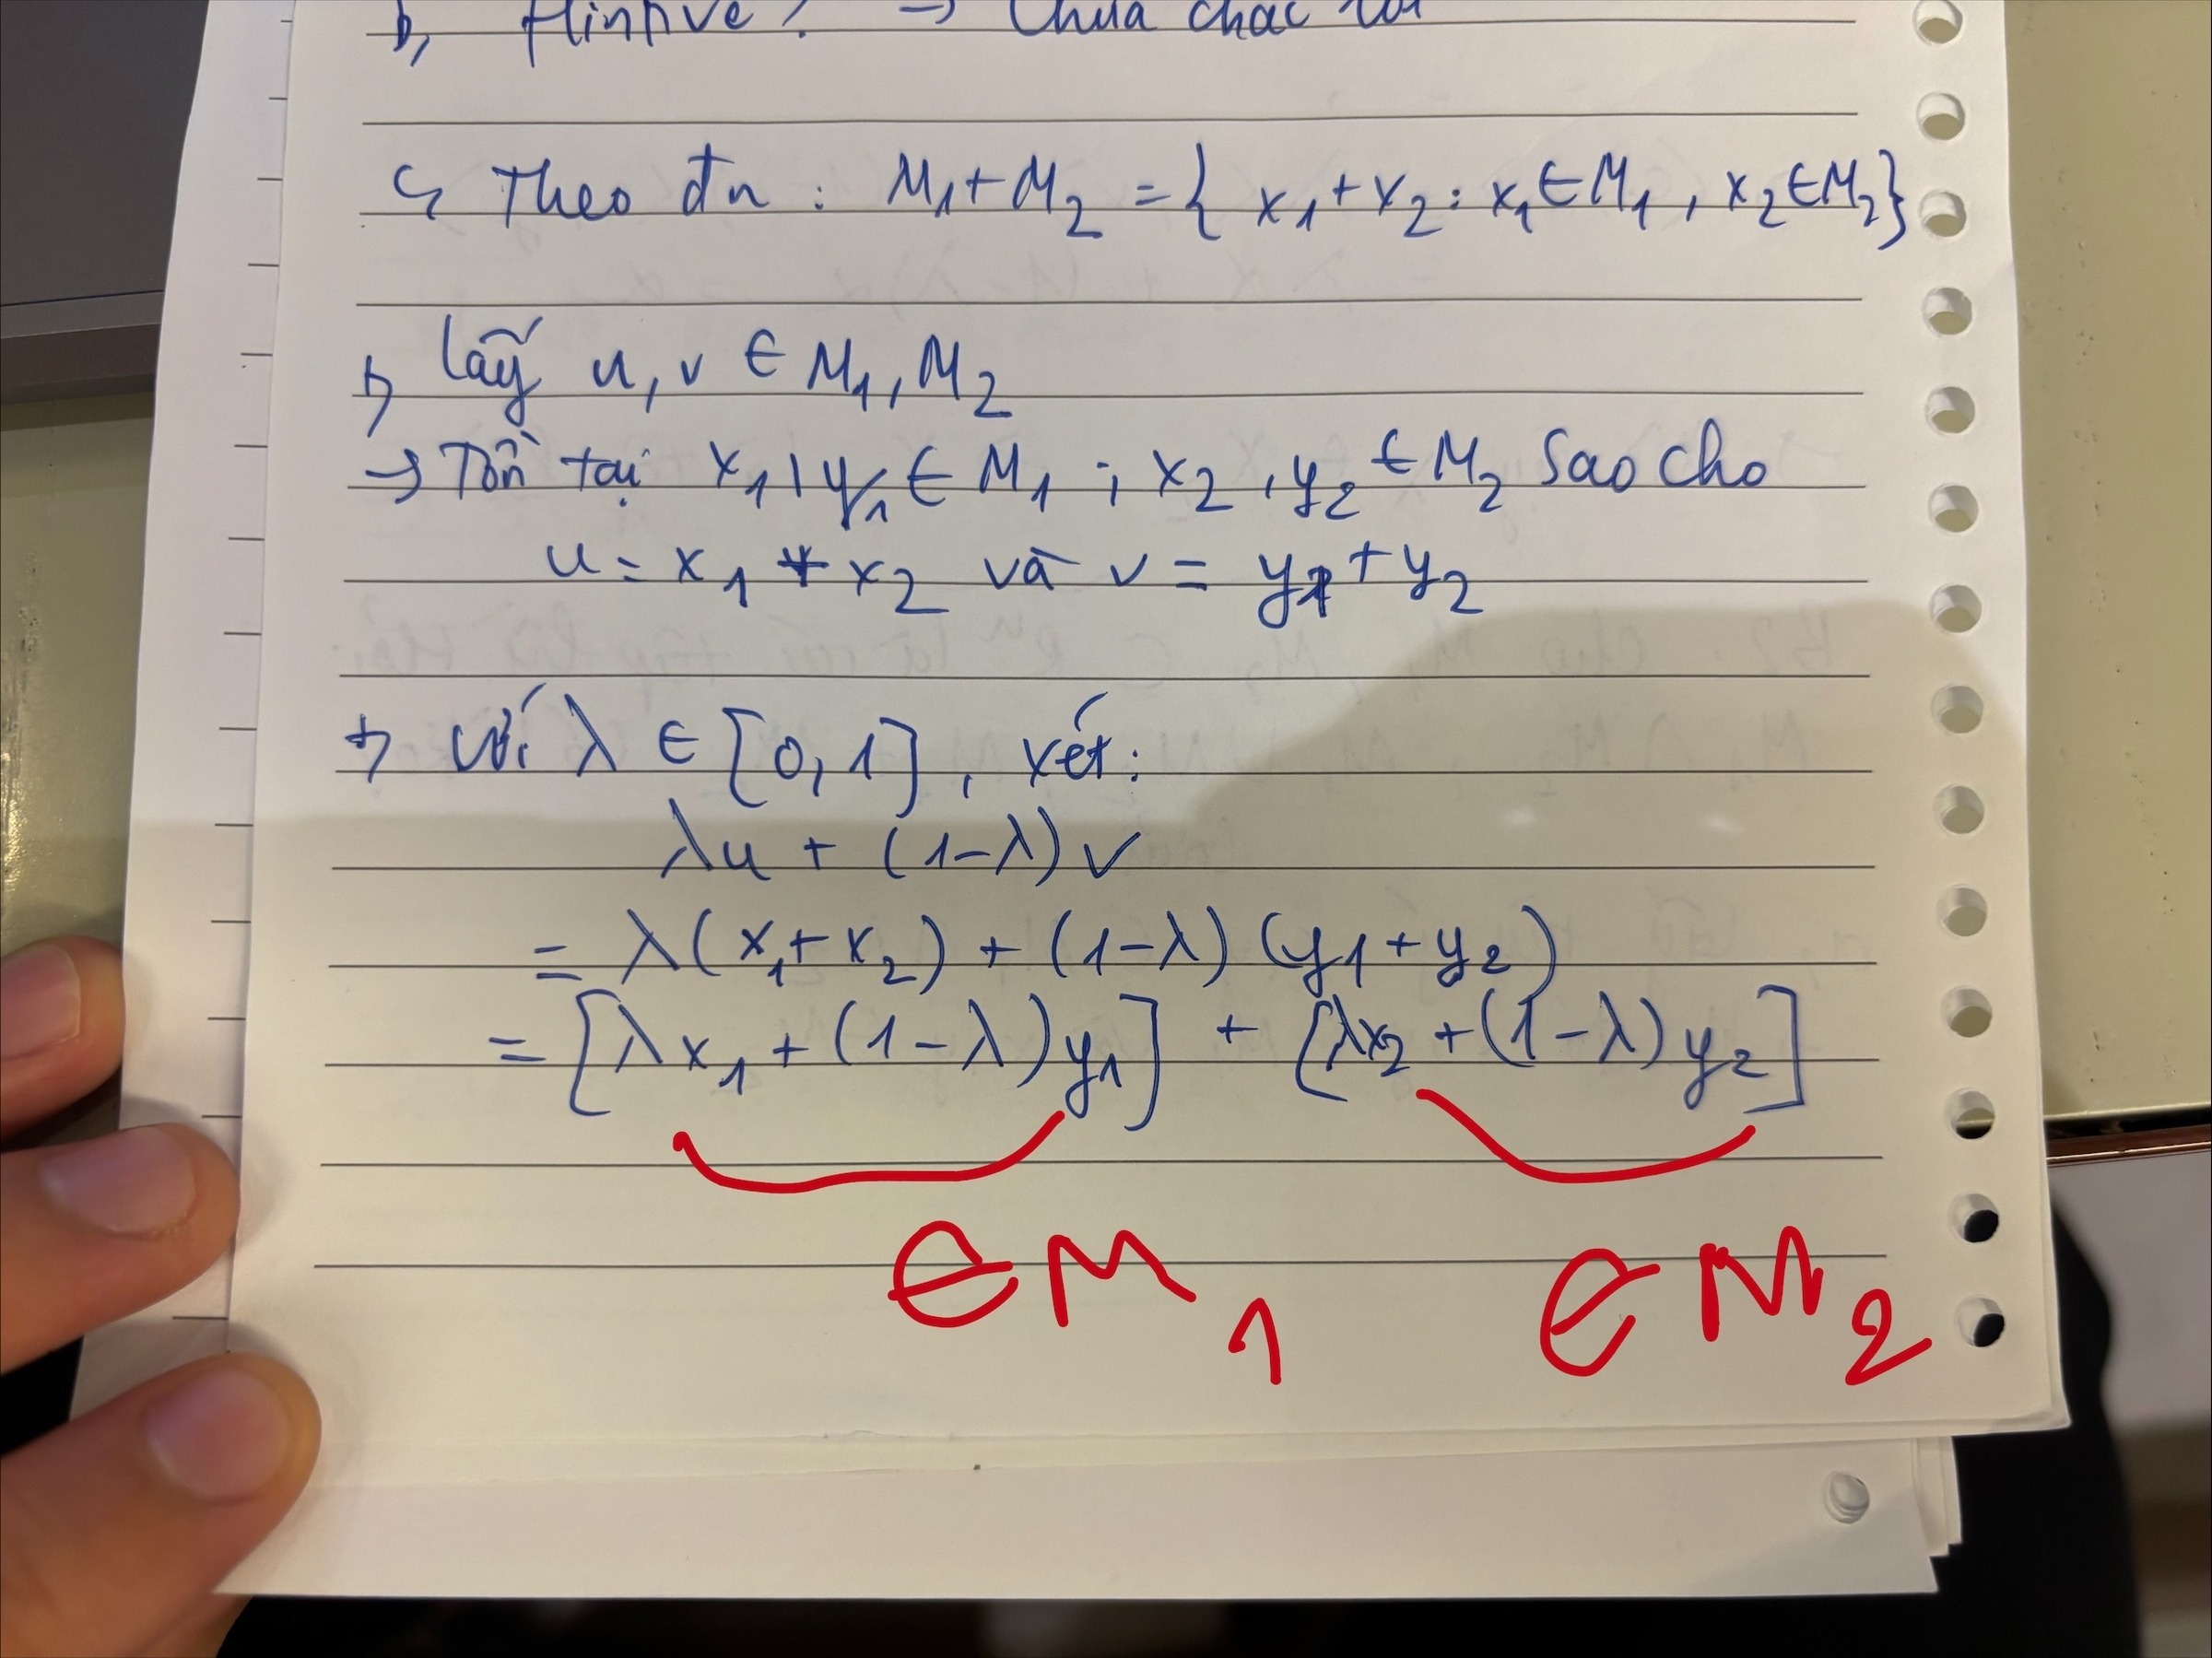
\includegraphics[width=.98\textwidth,height=.82\textheight,keepaspectratio]{bai_lam_them_1_assets/page-022.jpg}\end{center}
\clearpage
\phantomsection\label{src:023}
\noindent\textbf{Ảnh nguồn 023}\par\medskip
\begin{center}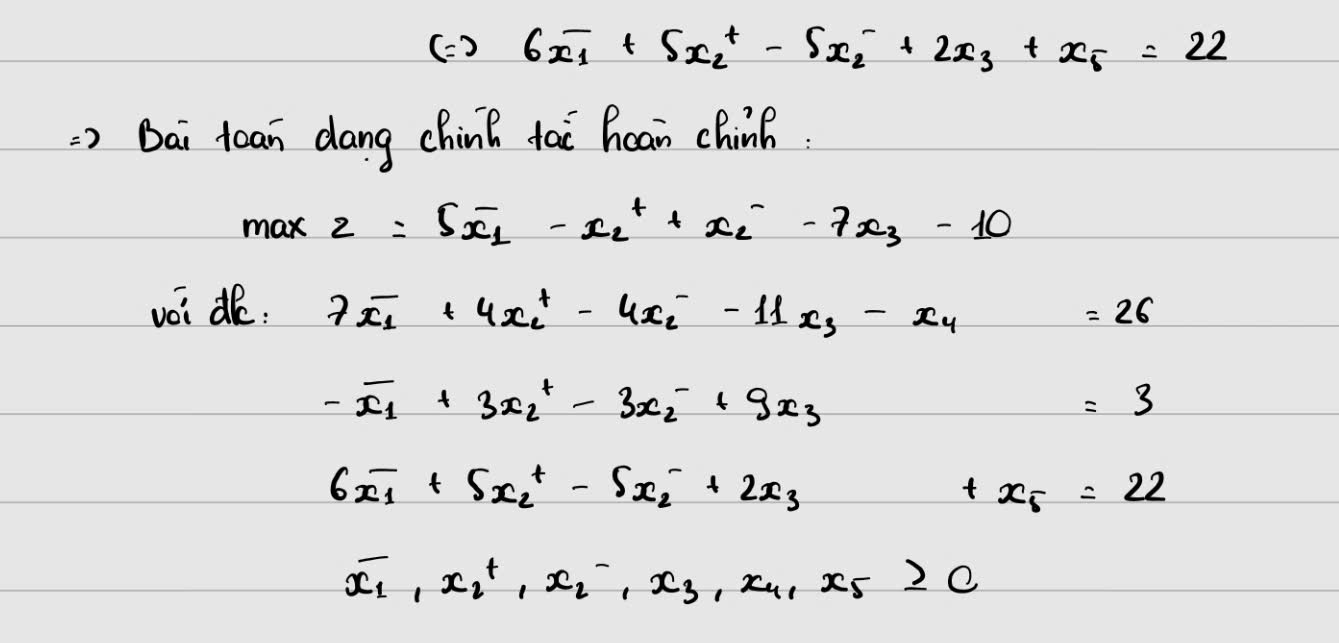
\includegraphics[width=.98\textwidth,height=.82\textheight,keepaspectratio]{bai_lam_them_1_assets/page-023.jpg}\end{center}
\clearpage
\phantomsection\label{src:024}
\noindent\textbf{Ảnh nguồn 024}\par\medskip
\begin{center}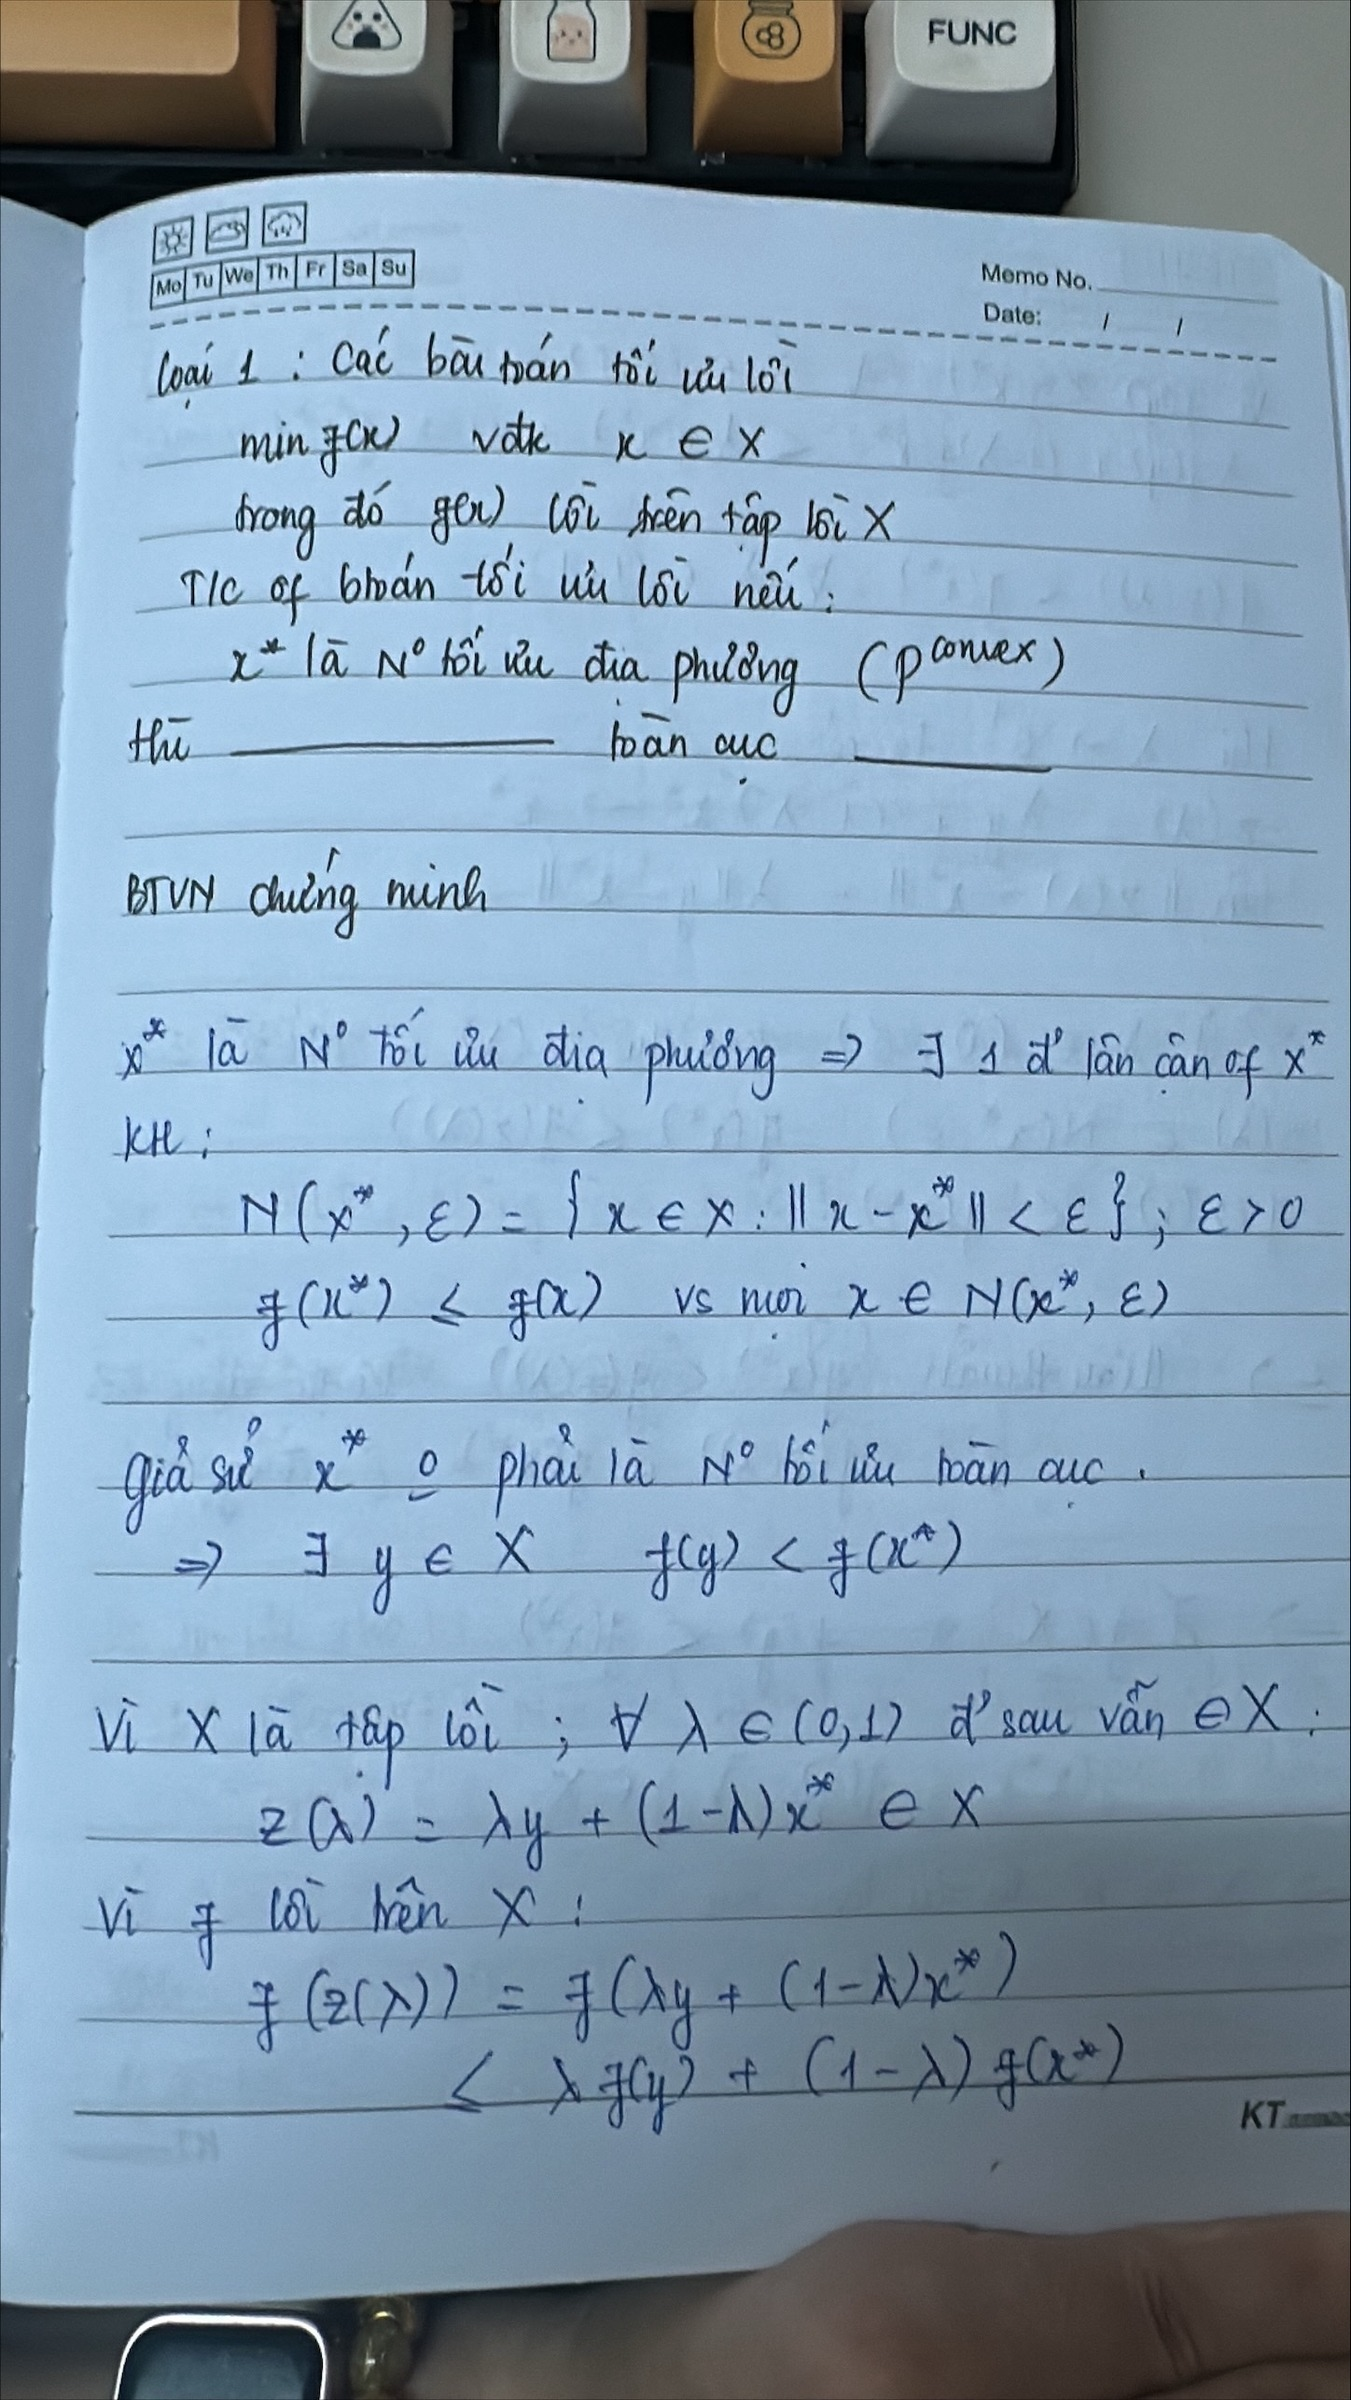
\includegraphics[width=.98\textwidth,height=.82\textheight,keepaspectratio]{bai_lam_them_1_assets/page-024.jpg}\end{center}
\clearpage
\phantomsection\label{src:025}
\noindent\textbf{Ảnh nguồn 025}\par\medskip
\begin{center}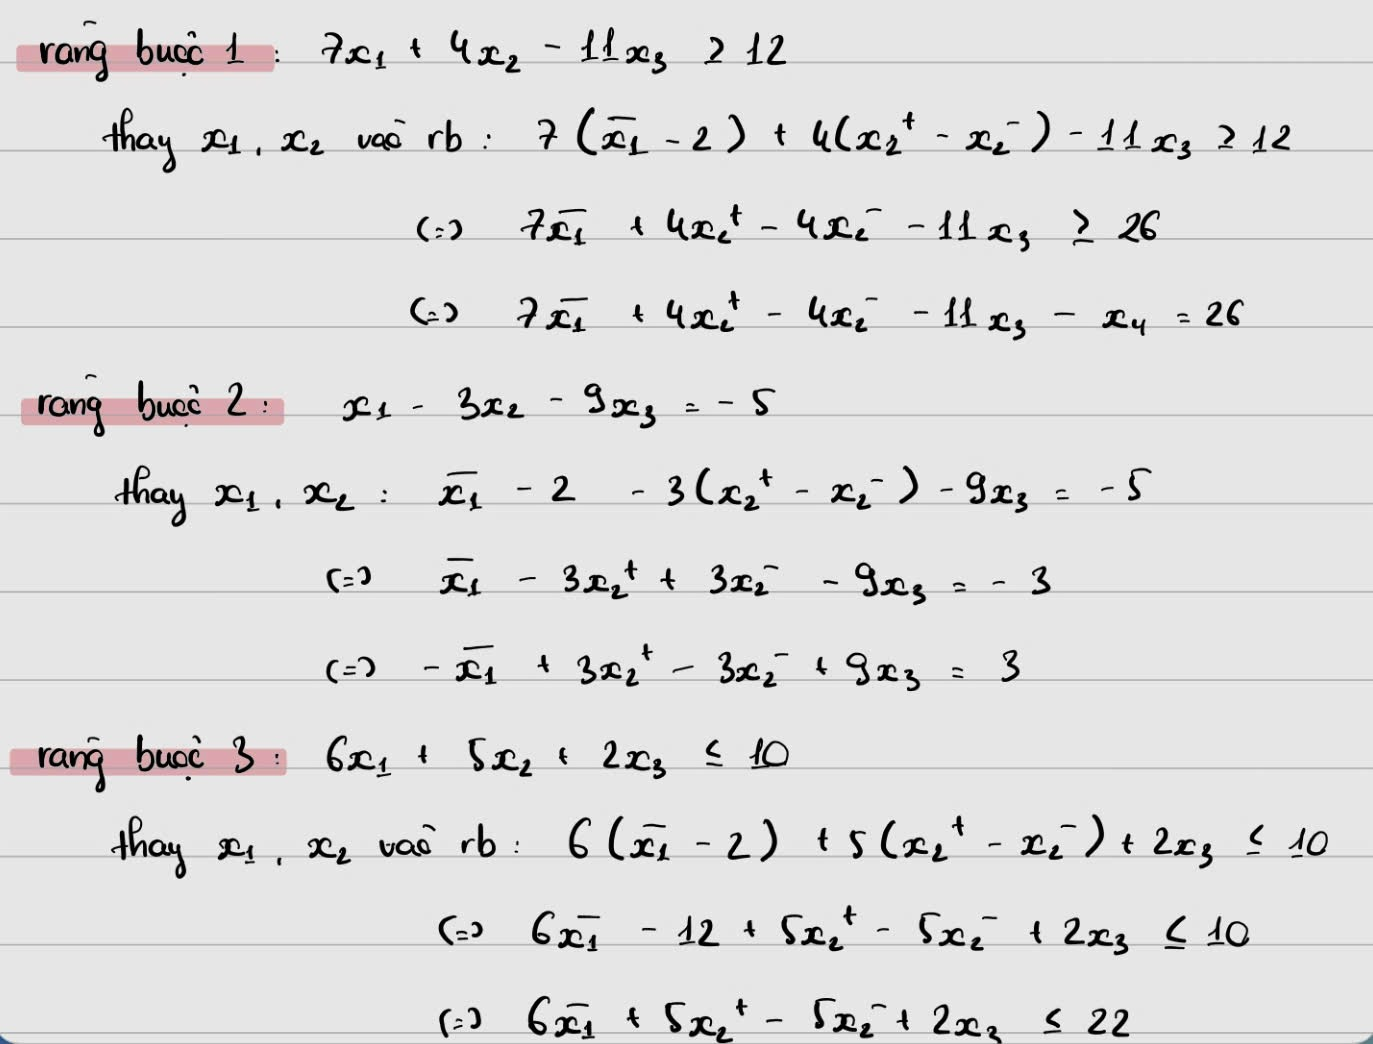
\includegraphics[width=.98\textwidth,height=.82\textheight,keepaspectratio]{bai_lam_them_1_assets/page-025.jpg}\end{center}
\clearpage
\phantomsection\label{src:026}
\noindent\textbf{Ảnh nguồn 026}\par\medskip
\begin{center}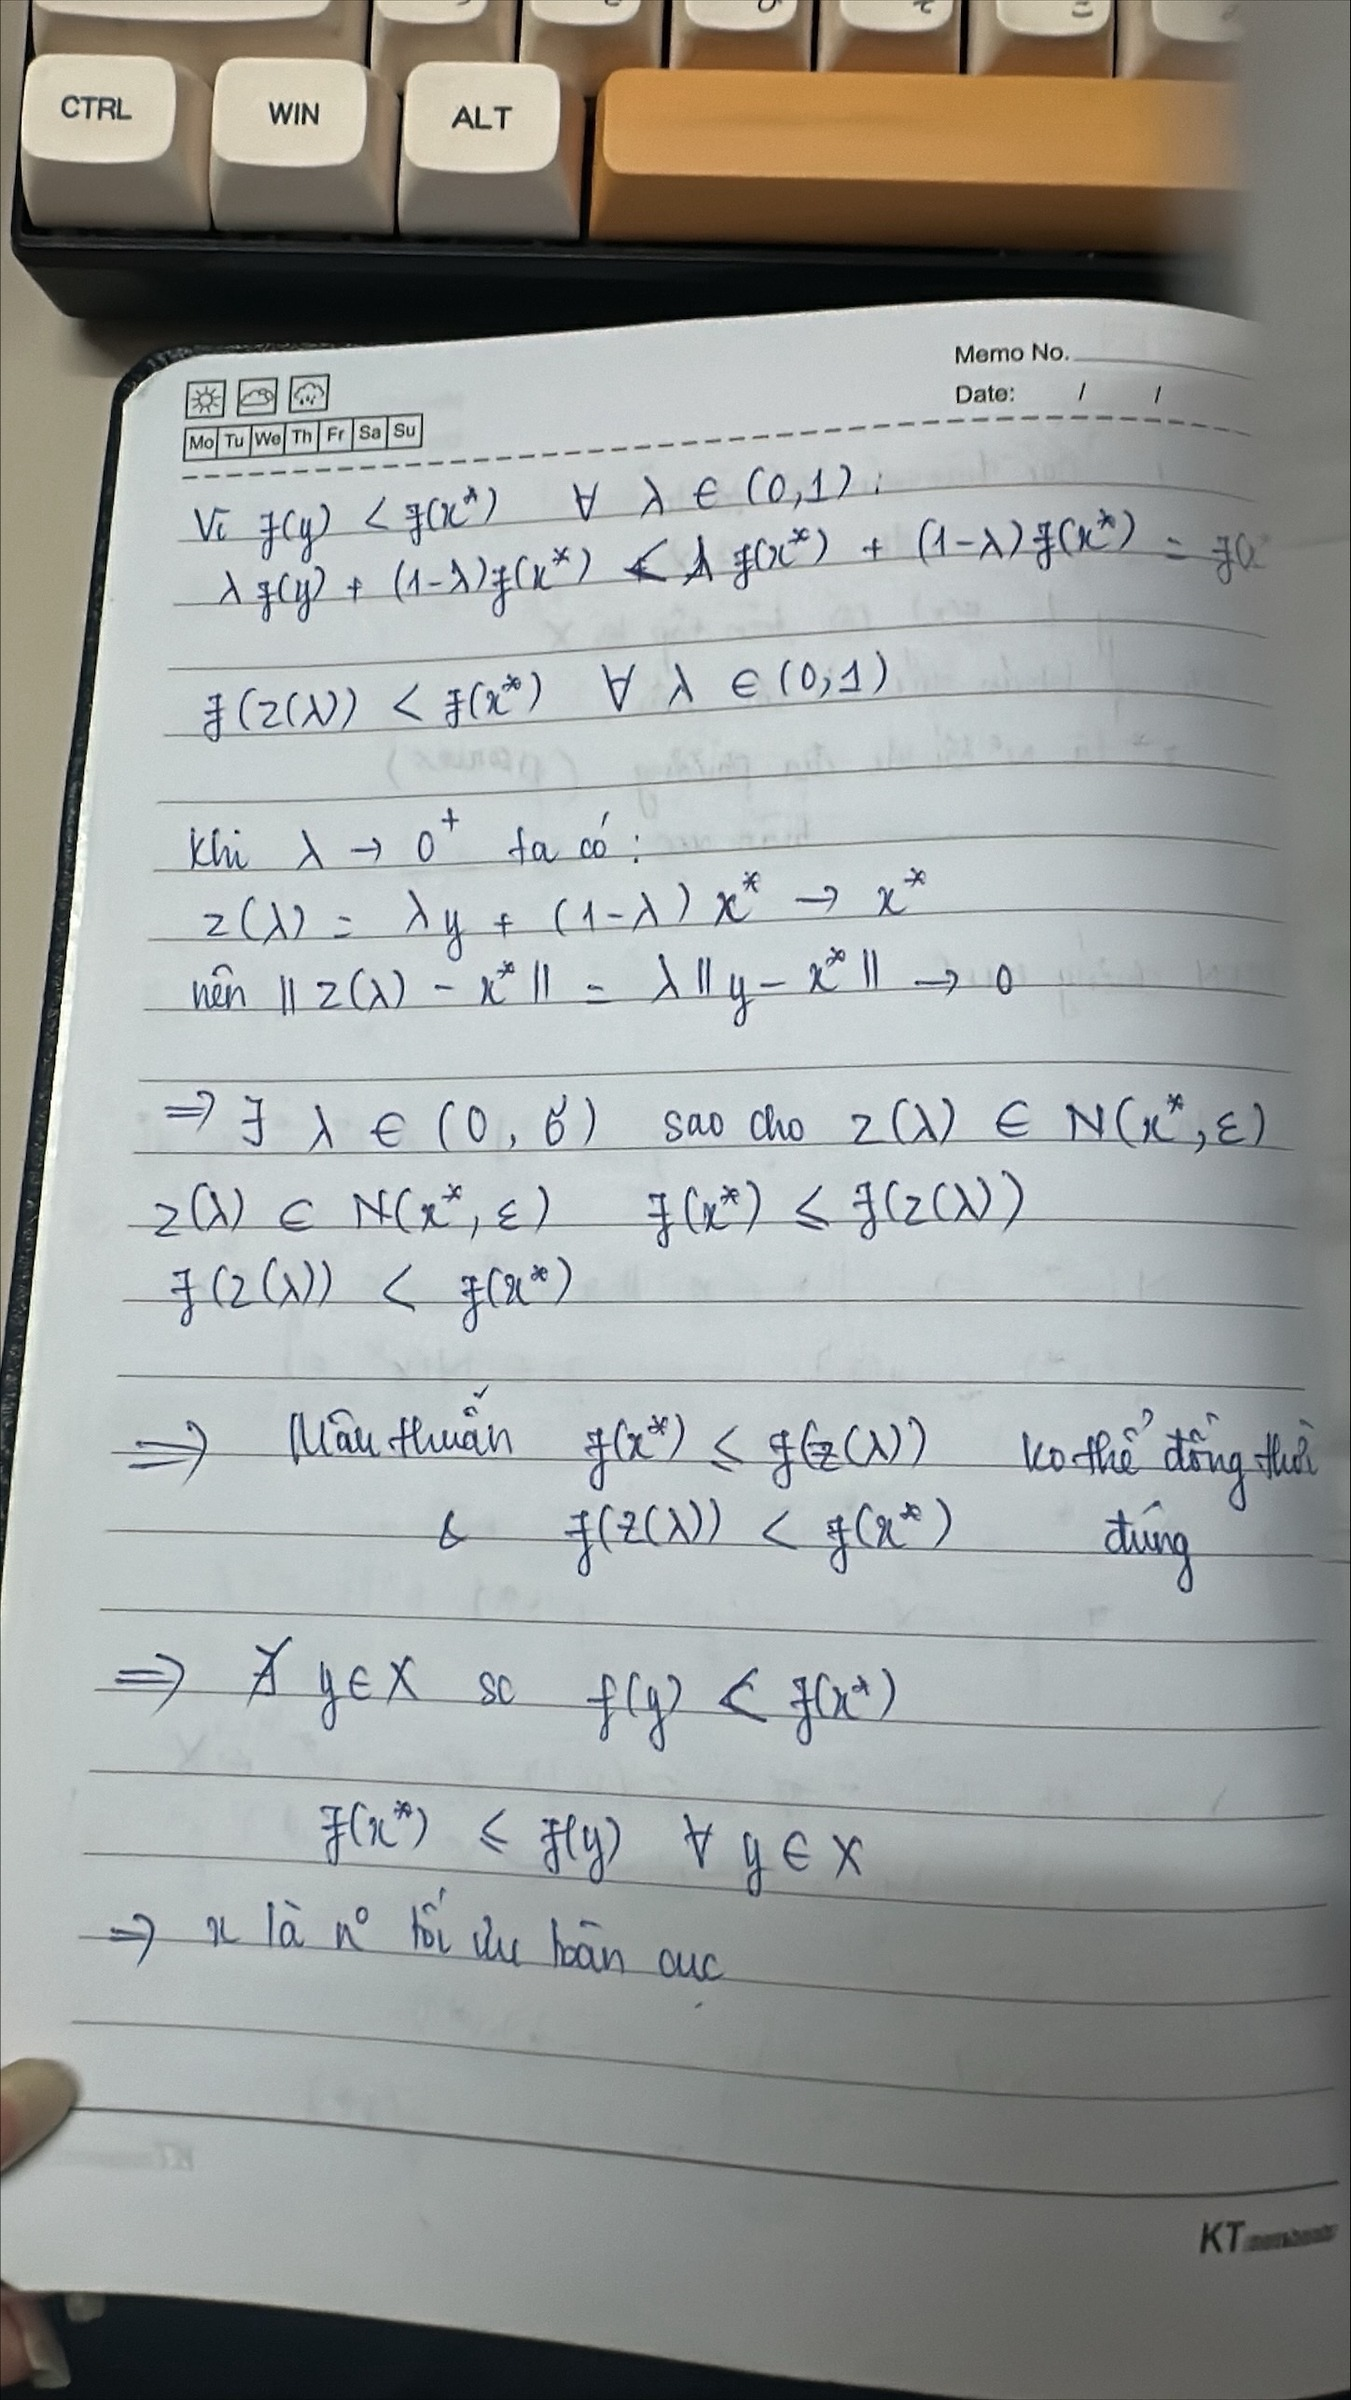
\includegraphics[width=.98\textwidth,height=.82\textheight,keepaspectratio]{bai_lam_them_1_assets/page-026.jpg}\end{center}
\clearpage
\phantomsection\label{src:027}
\noindent\textbf{Ảnh nguồn 027}\par\medskip
\begin{center}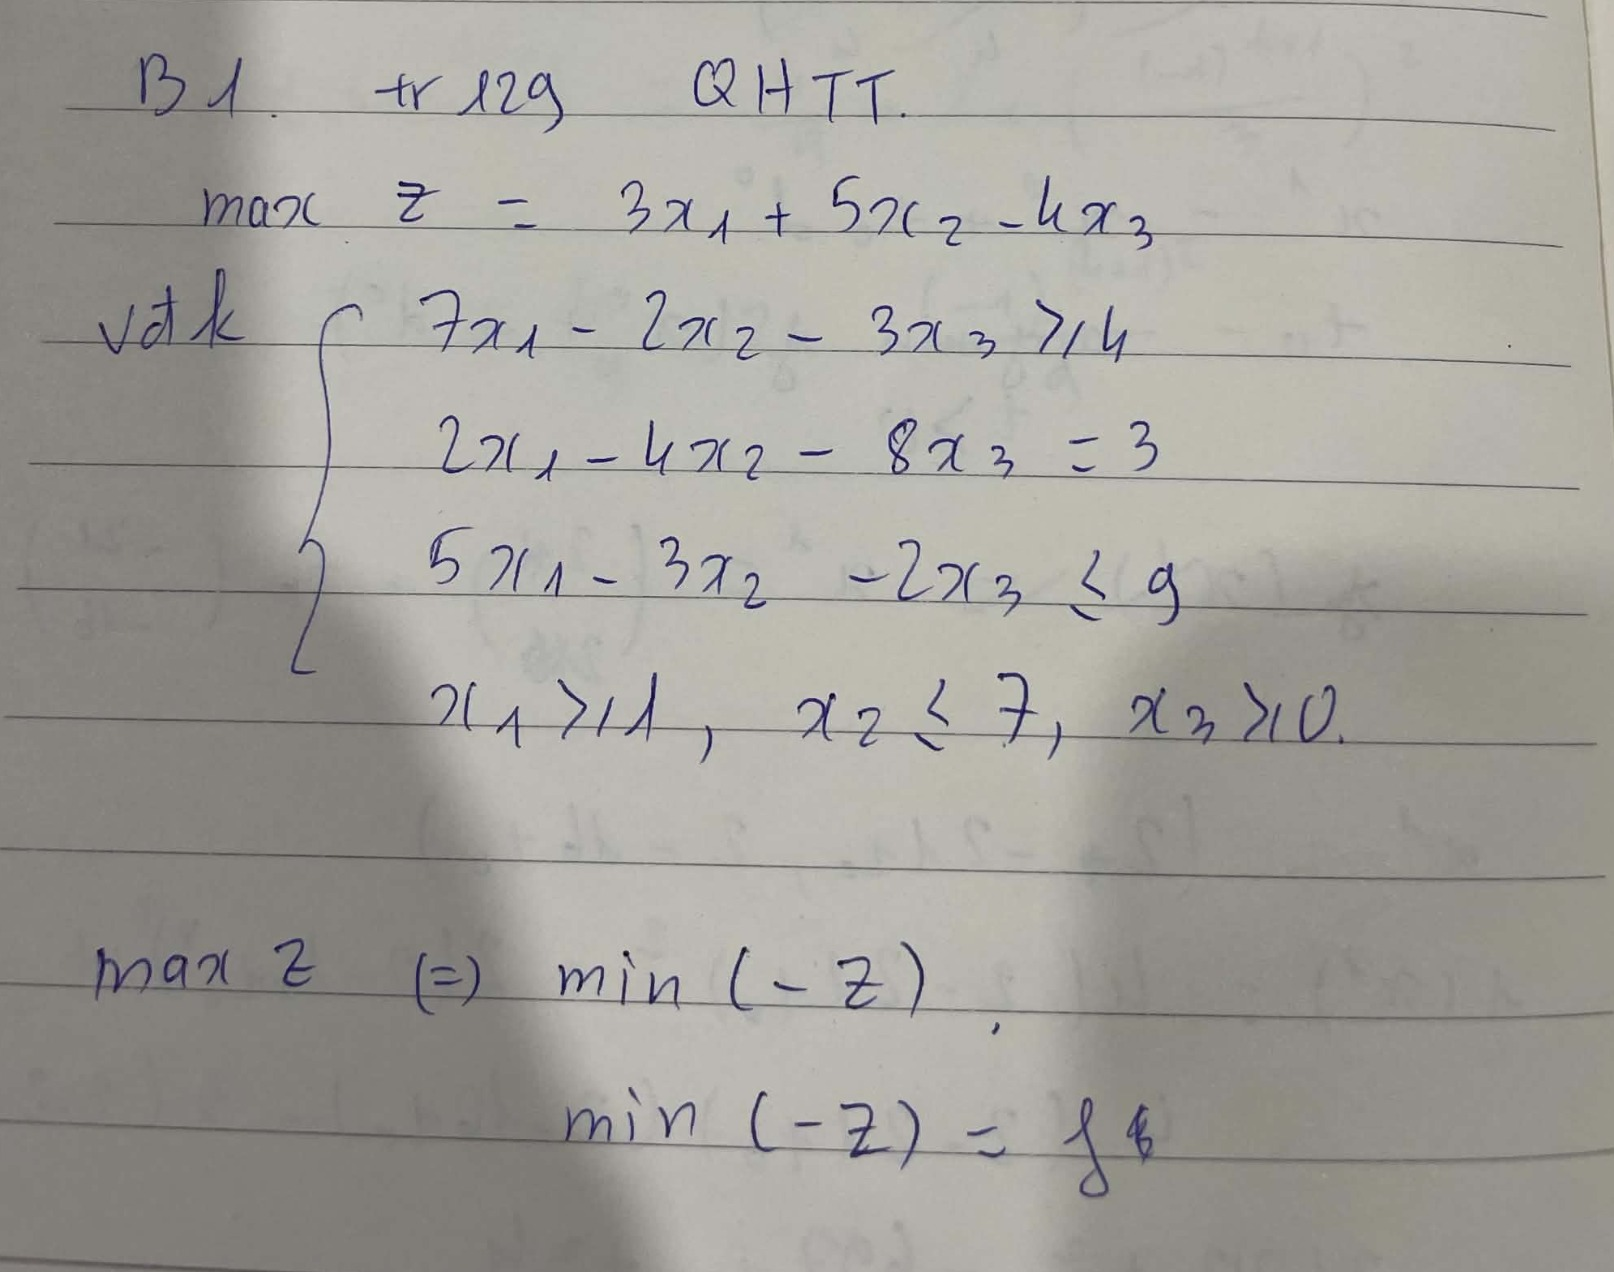
\includegraphics[width=.98\textwidth,height=.82\textheight,keepaspectratio]{bai_lam_them_1_assets/page-027.jpg}\end{center}
\clearpage
\phantomsection\label{src:028}
\noindent\textbf{Ảnh nguồn 028}\par\medskip
\begin{center}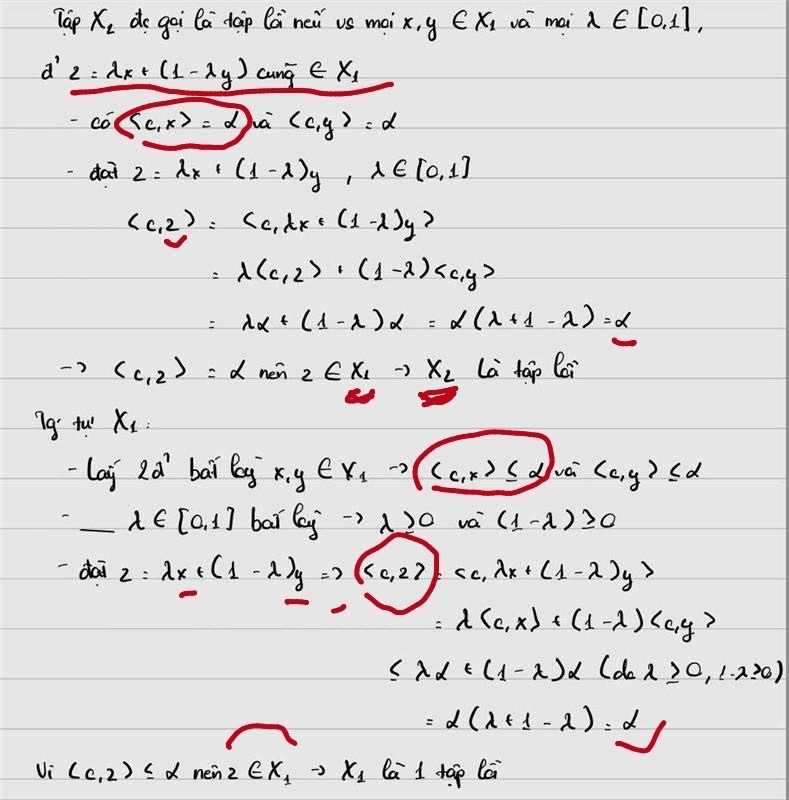
\includegraphics[width=.98\textwidth,height=.82\textheight,keepaspectratio]{bai_lam_them_1_assets/page-028.jpg}\end{center}
\clearpage
\phantomsection\label{src:029}
\noindent\textbf{Ảnh nguồn 029}\par\medskip
\begin{center}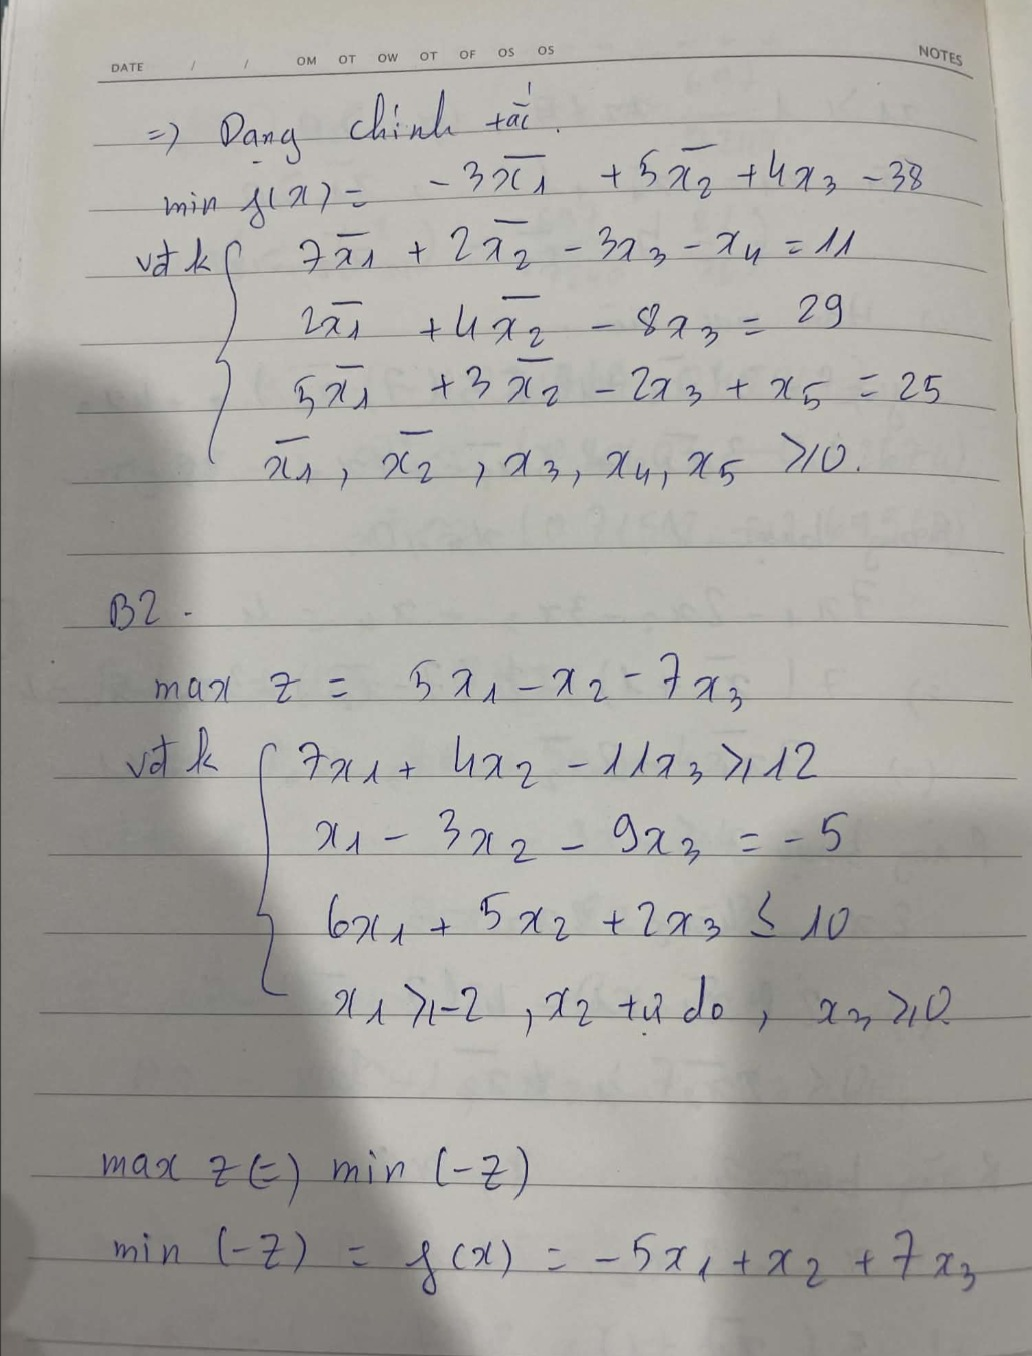
\includegraphics[width=.98\textwidth,height=.82\textheight,keepaspectratio]{bai_lam_them_1_assets/page-029.jpg}\end{center}
\clearpage
\phantomsection\label{src:030}
\noindent\textbf{Ảnh nguồn 030}\par\medskip
\begin{center}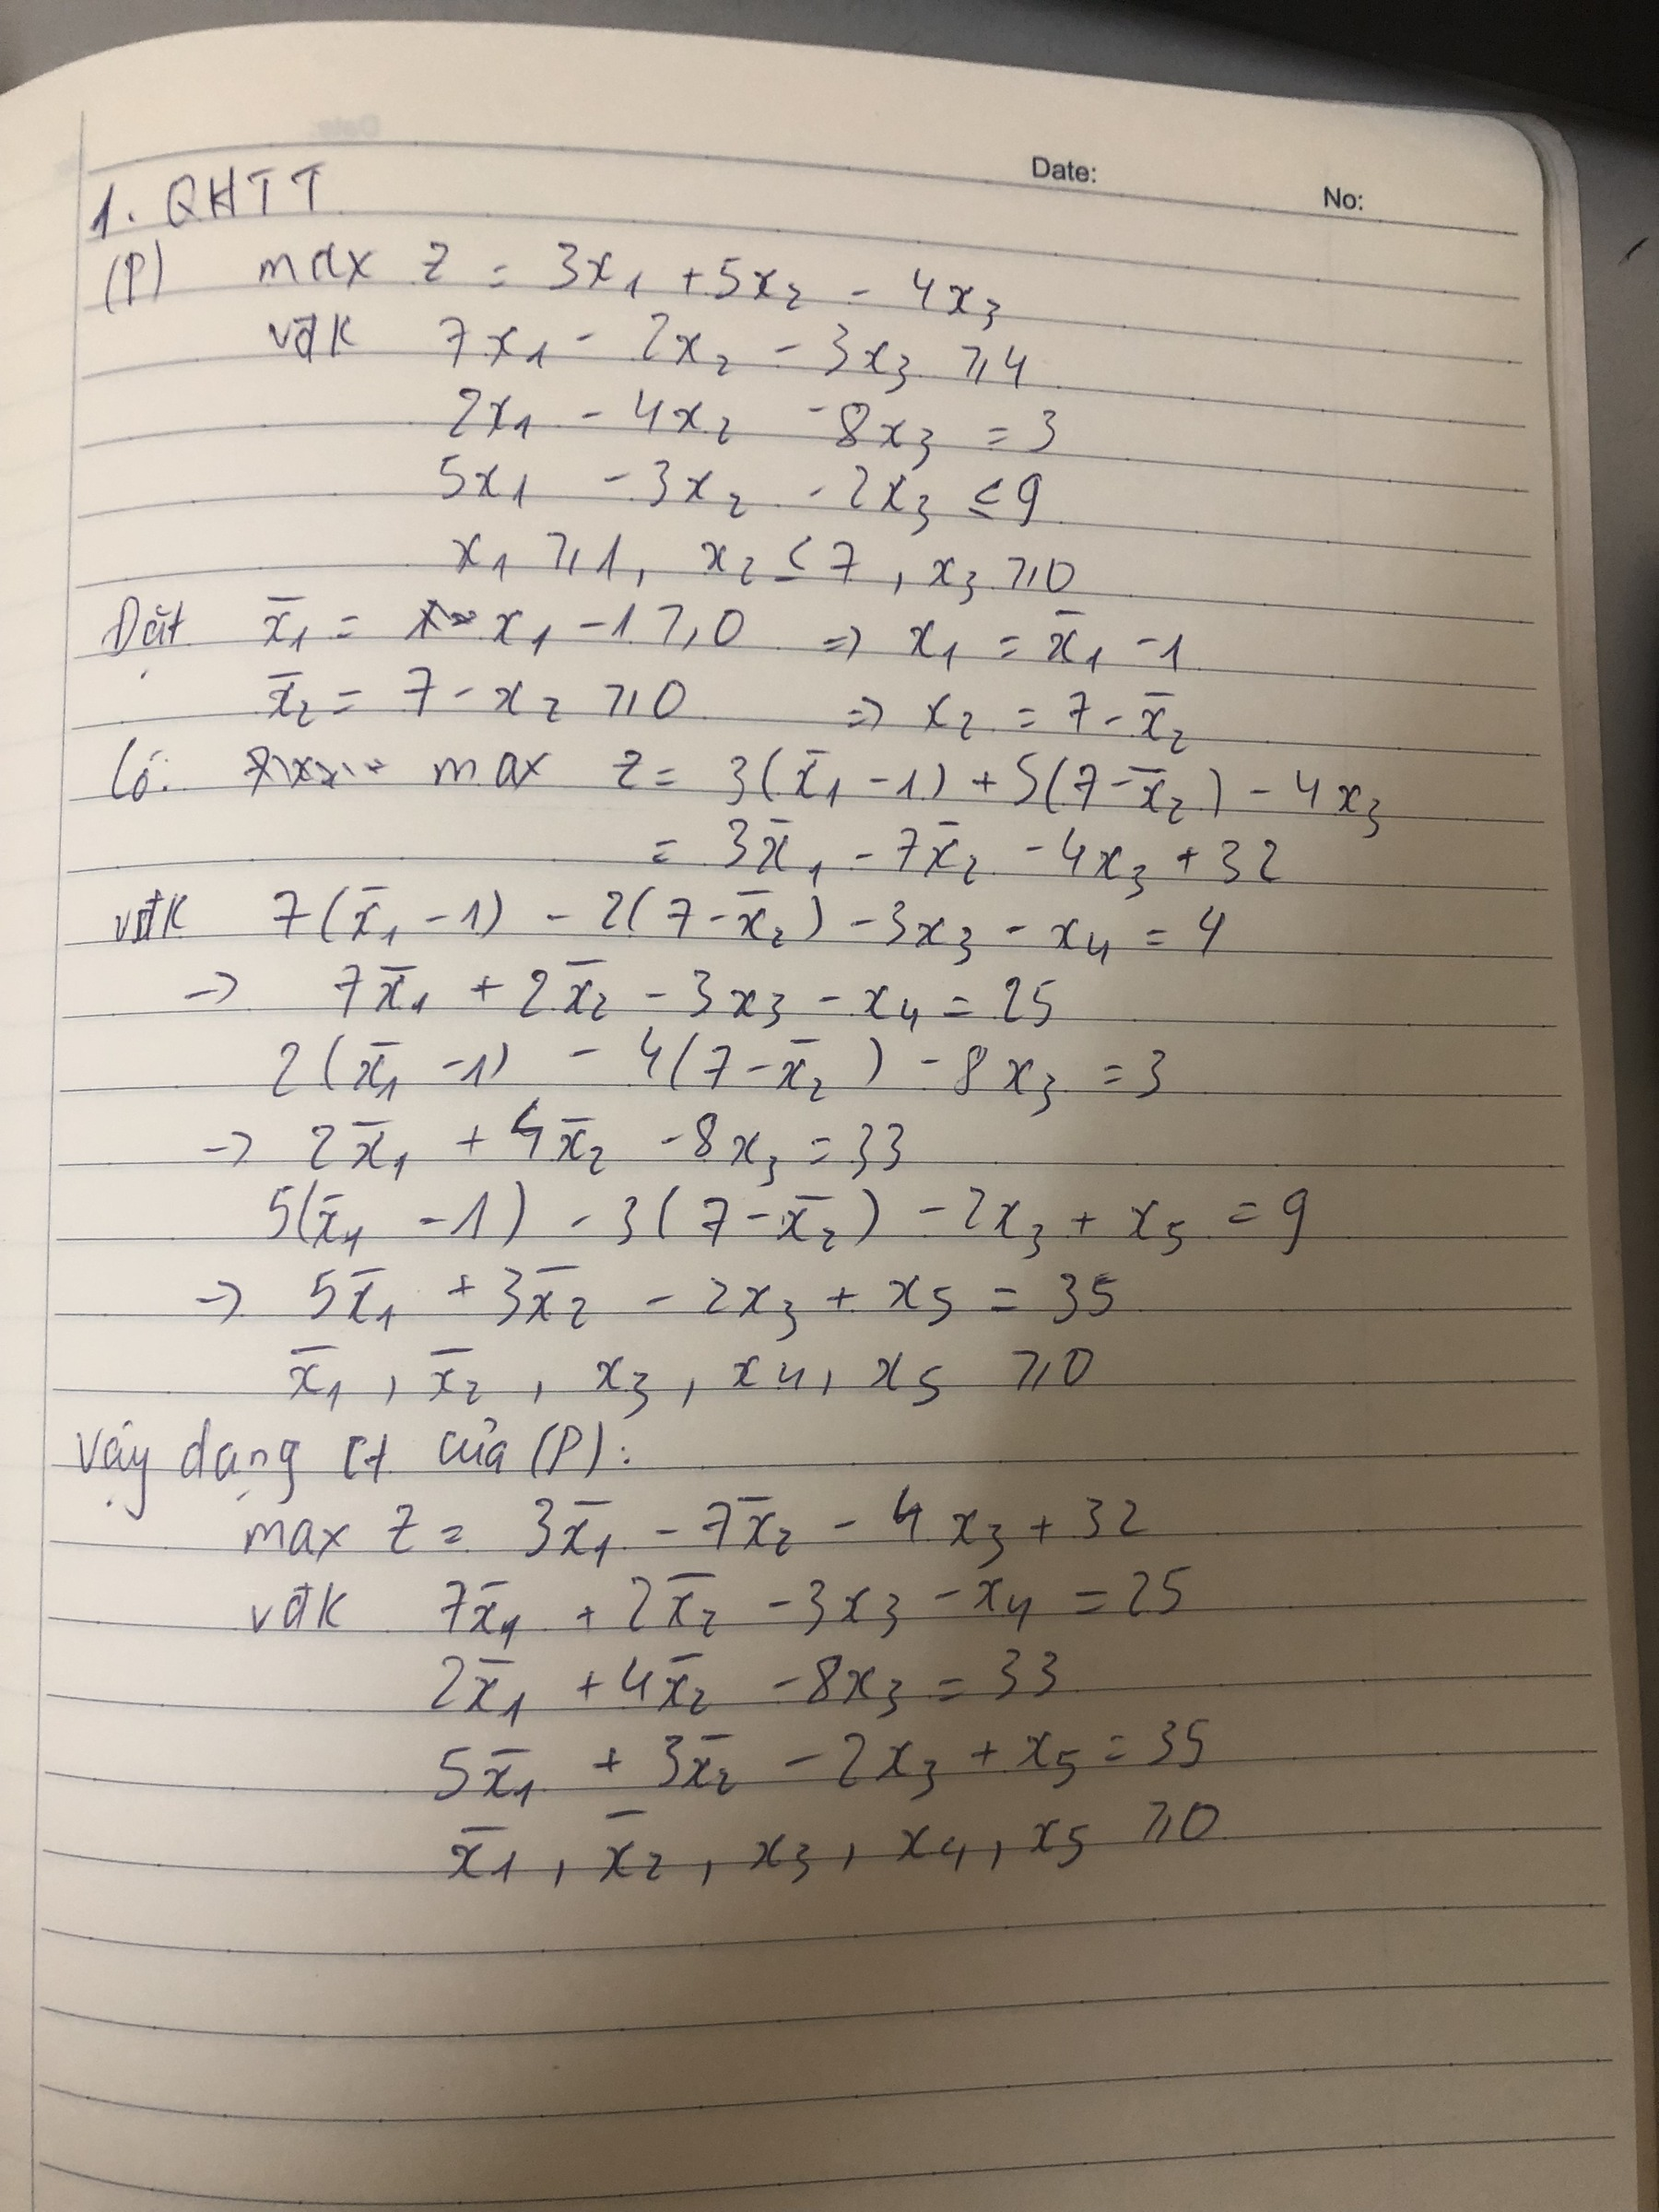
\includegraphics[width=.98\textwidth,height=.82\textheight,keepaspectratio]{bai_lam_them_1_assets/page-030.jpg}\end{center}
\clearpage
\phantomsection\label{src:031}
\noindent\textbf{Ảnh nguồn 031}\par\medskip
\begin{center}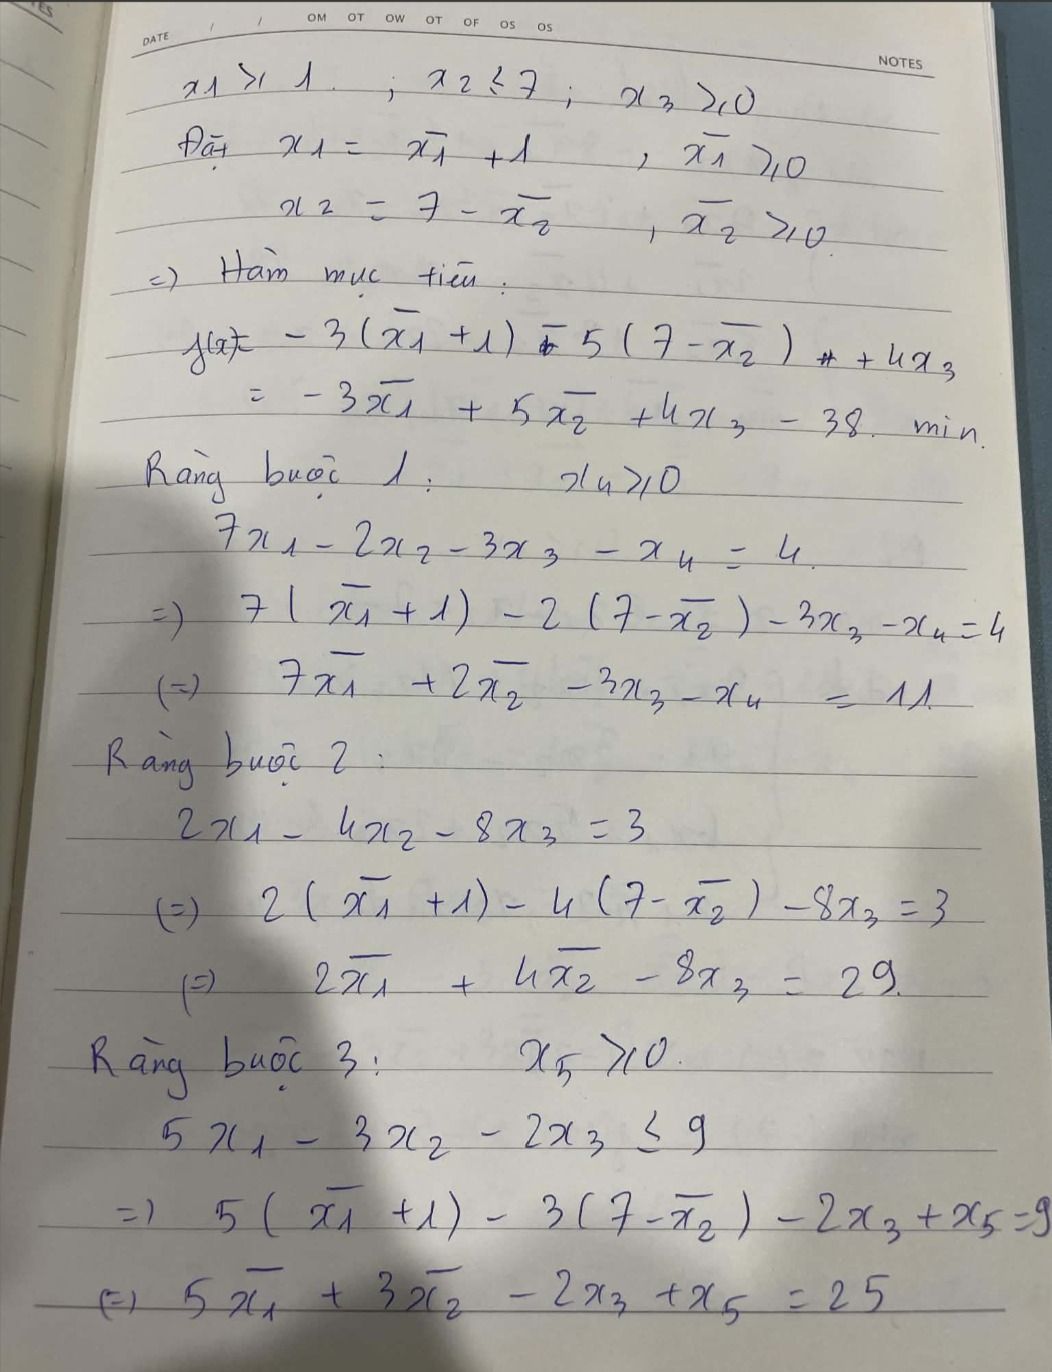
\includegraphics[width=.98\textwidth,height=.82\textheight,keepaspectratio]{bai_lam_them_1_assets/page-031.jpg}\end{center}
\clearpage
\phantomsection\label{src:032}
\noindent\textbf{Ảnh nguồn 032}\par\medskip
\begin{center}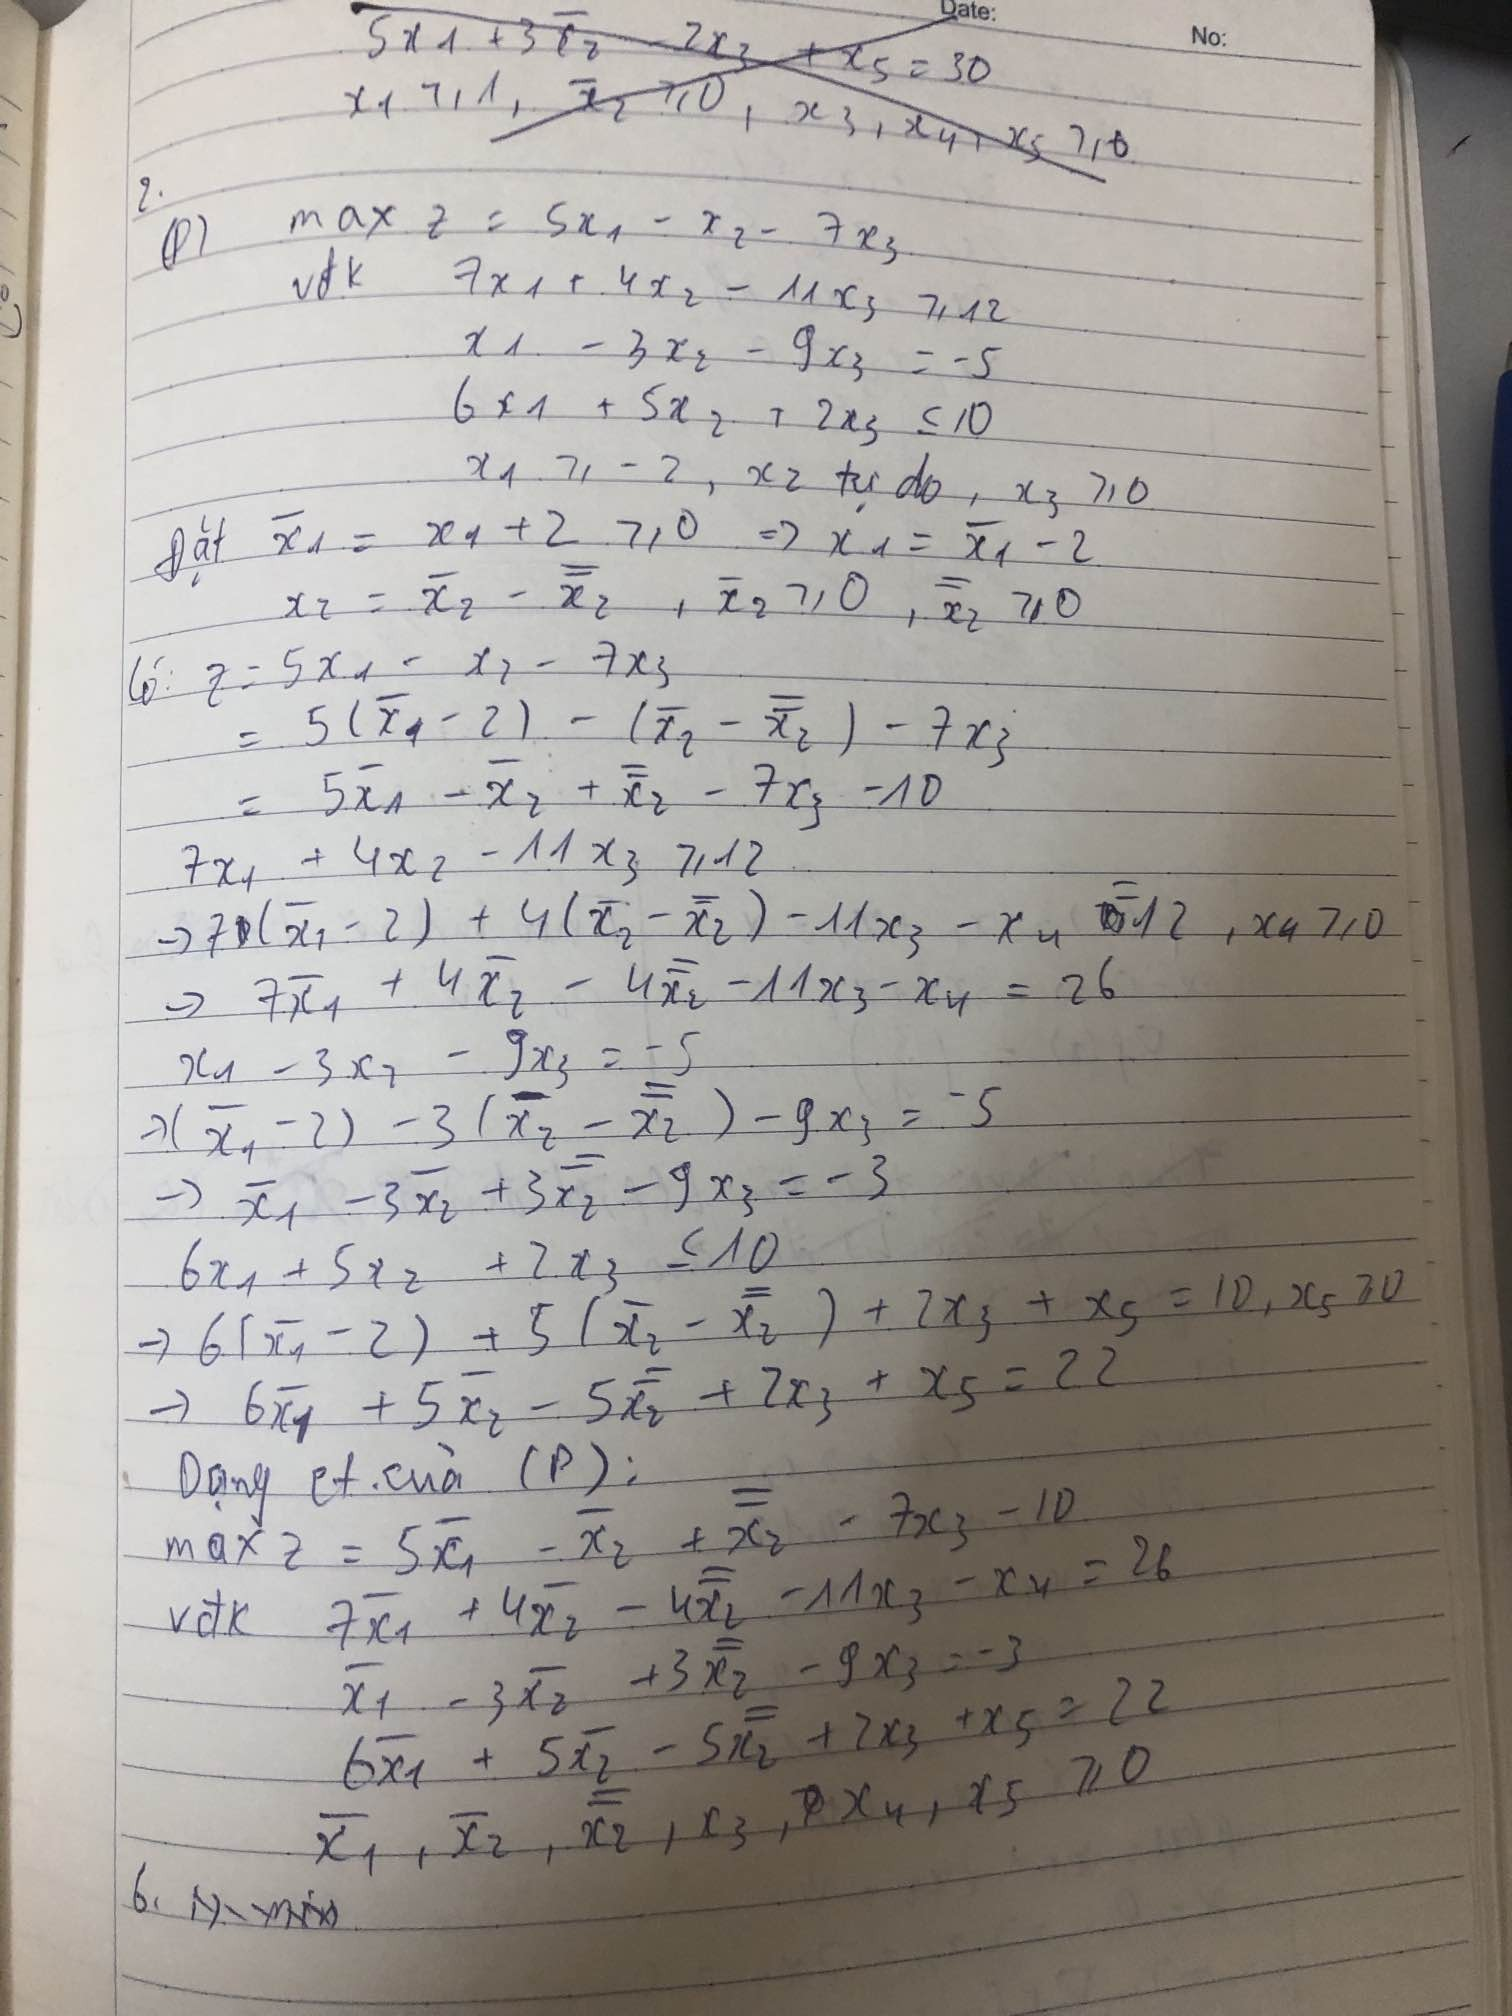
\includegraphics[width=.98\textwidth,height=.82\textheight,keepaspectratio]{bai_lam_them_1_assets/page-032.jpg}\end{center}
\clearpage
\phantomsection\label{src:033}
\noindent\textbf{Ảnh nguồn 033}\par\medskip
\begin{center}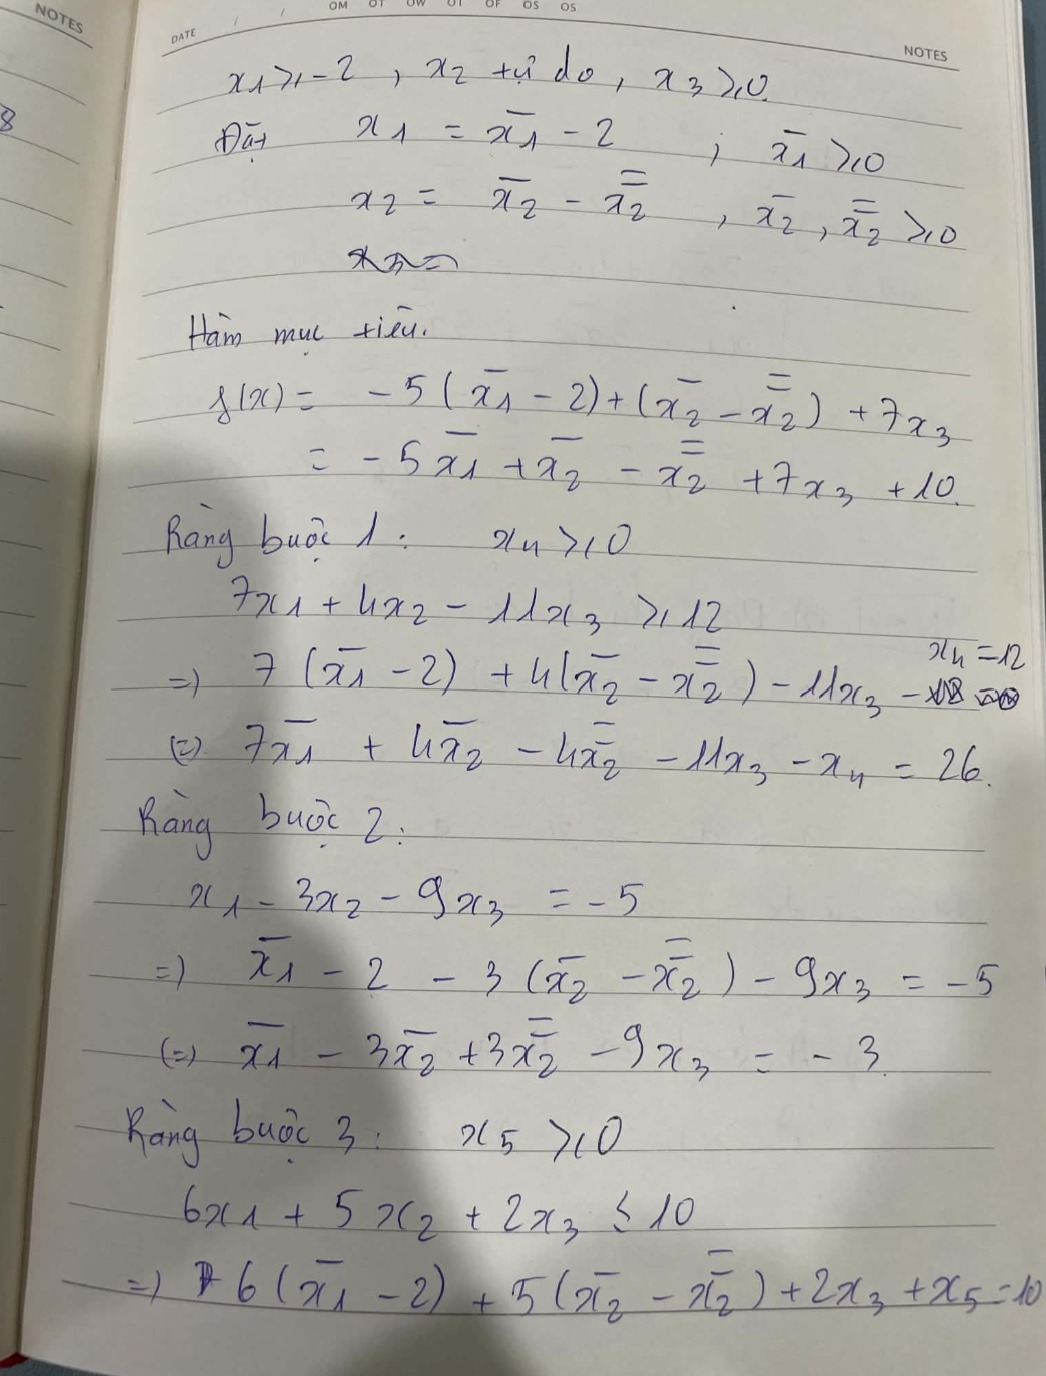
\includegraphics[width=.98\textwidth,height=.82\textheight,keepaspectratio]{bai_lam_them_1_assets/page-033.jpg}\end{center}
\clearpage
\phantomsection\label{src:034}
\noindent\textbf{Ảnh nguồn 034}\par\medskip
\begin{center}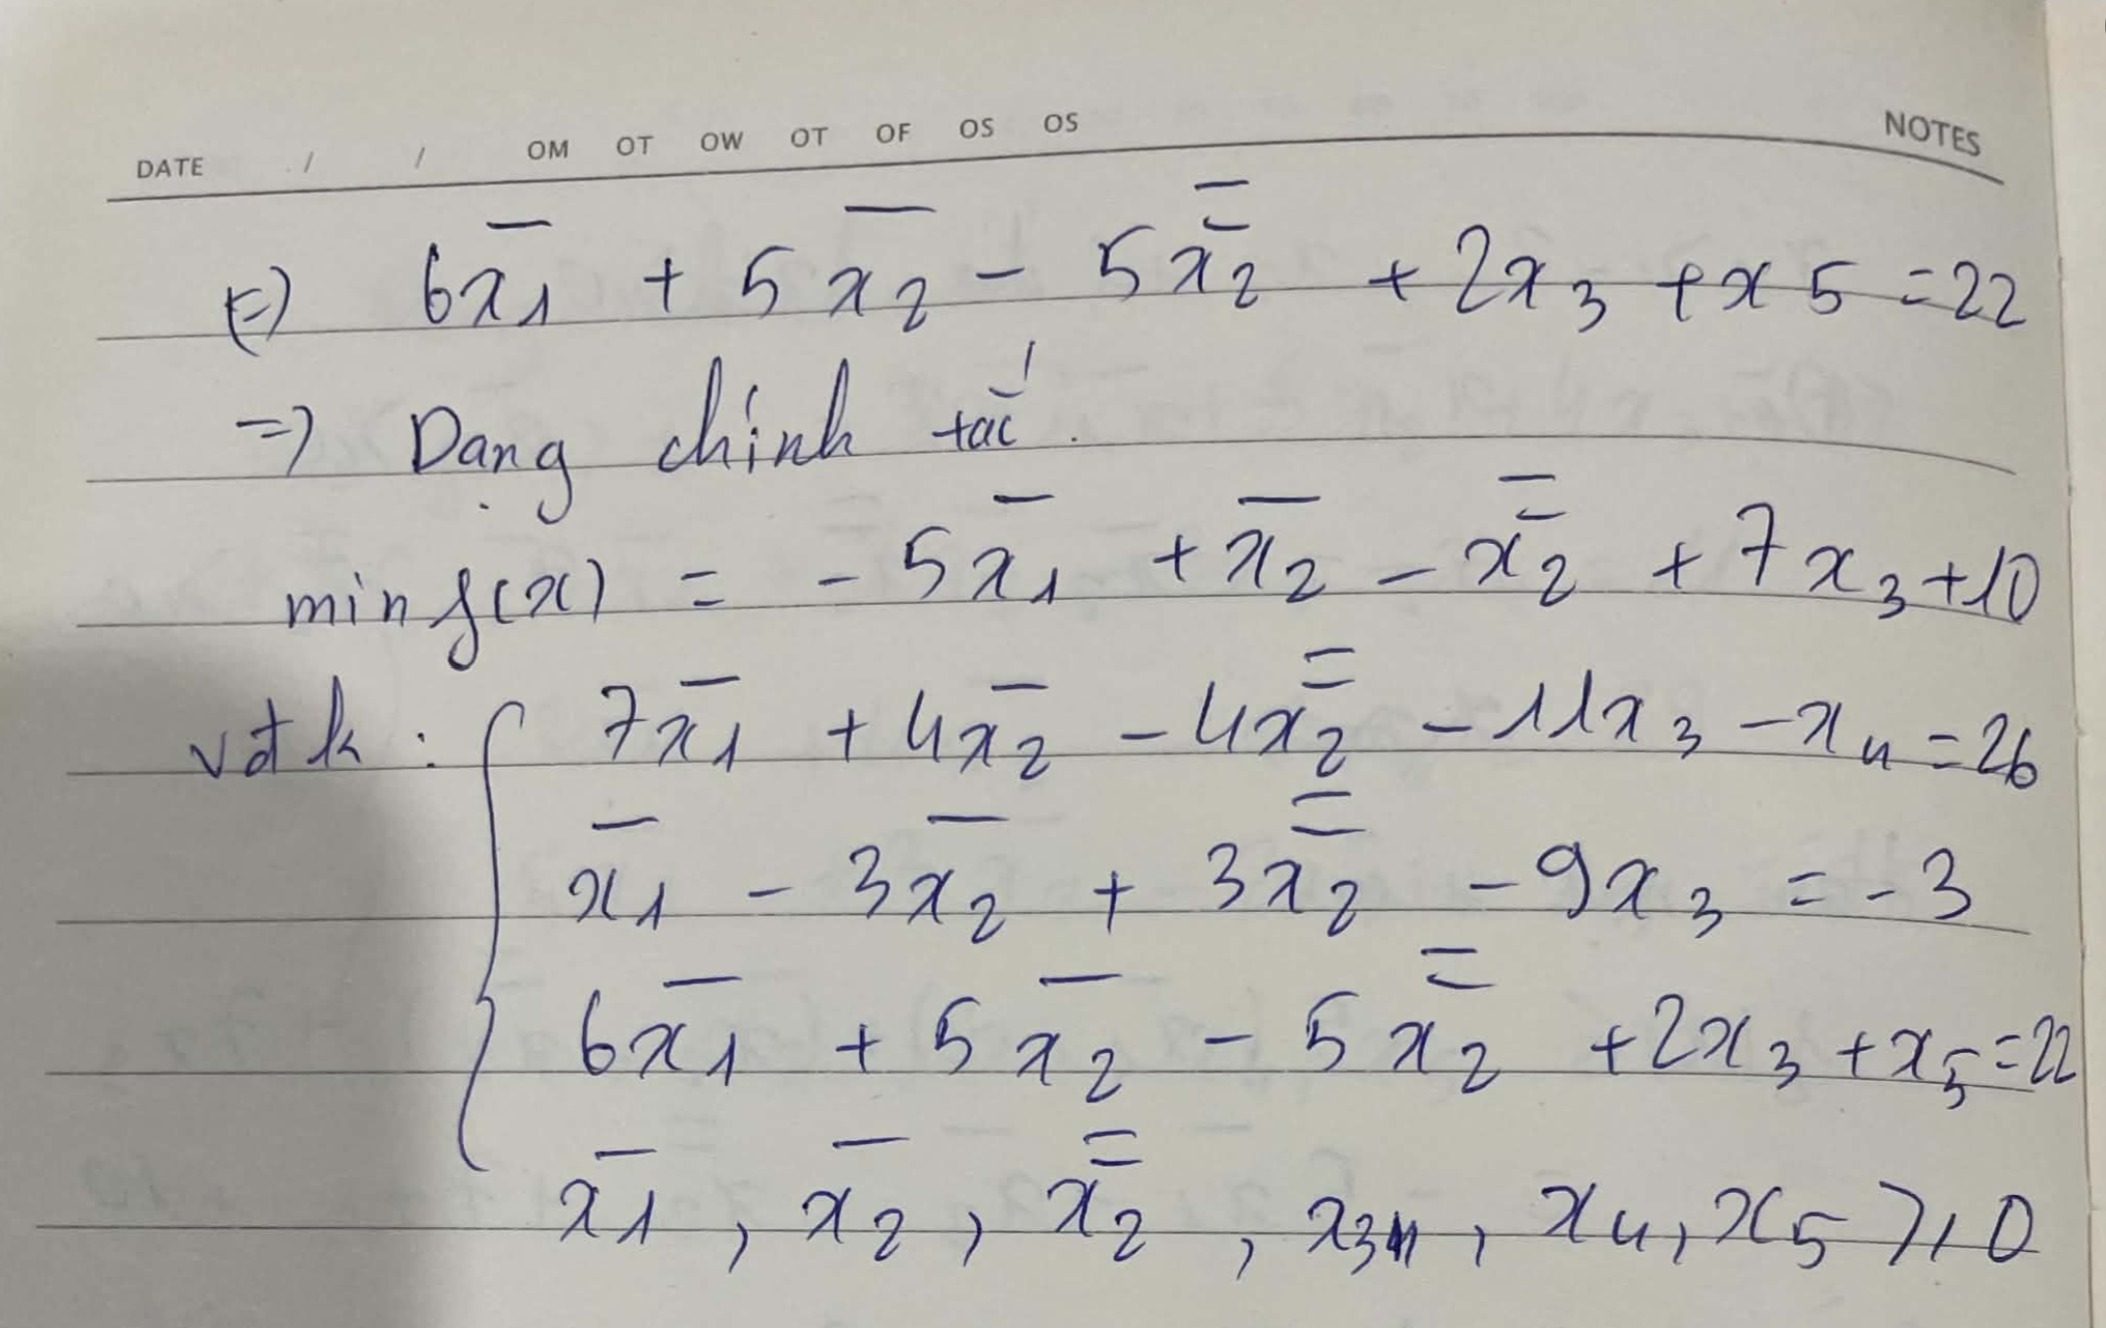
\includegraphics[width=.98\textwidth,height=.82\textheight,keepaspectratio]{bai_lam_them_1_assets/page-034.jpg}\end{center}
\clearpage
\phantomsection\label{src:035}
\noindent\textbf{Ảnh nguồn 035}\par\medskip
\begin{center}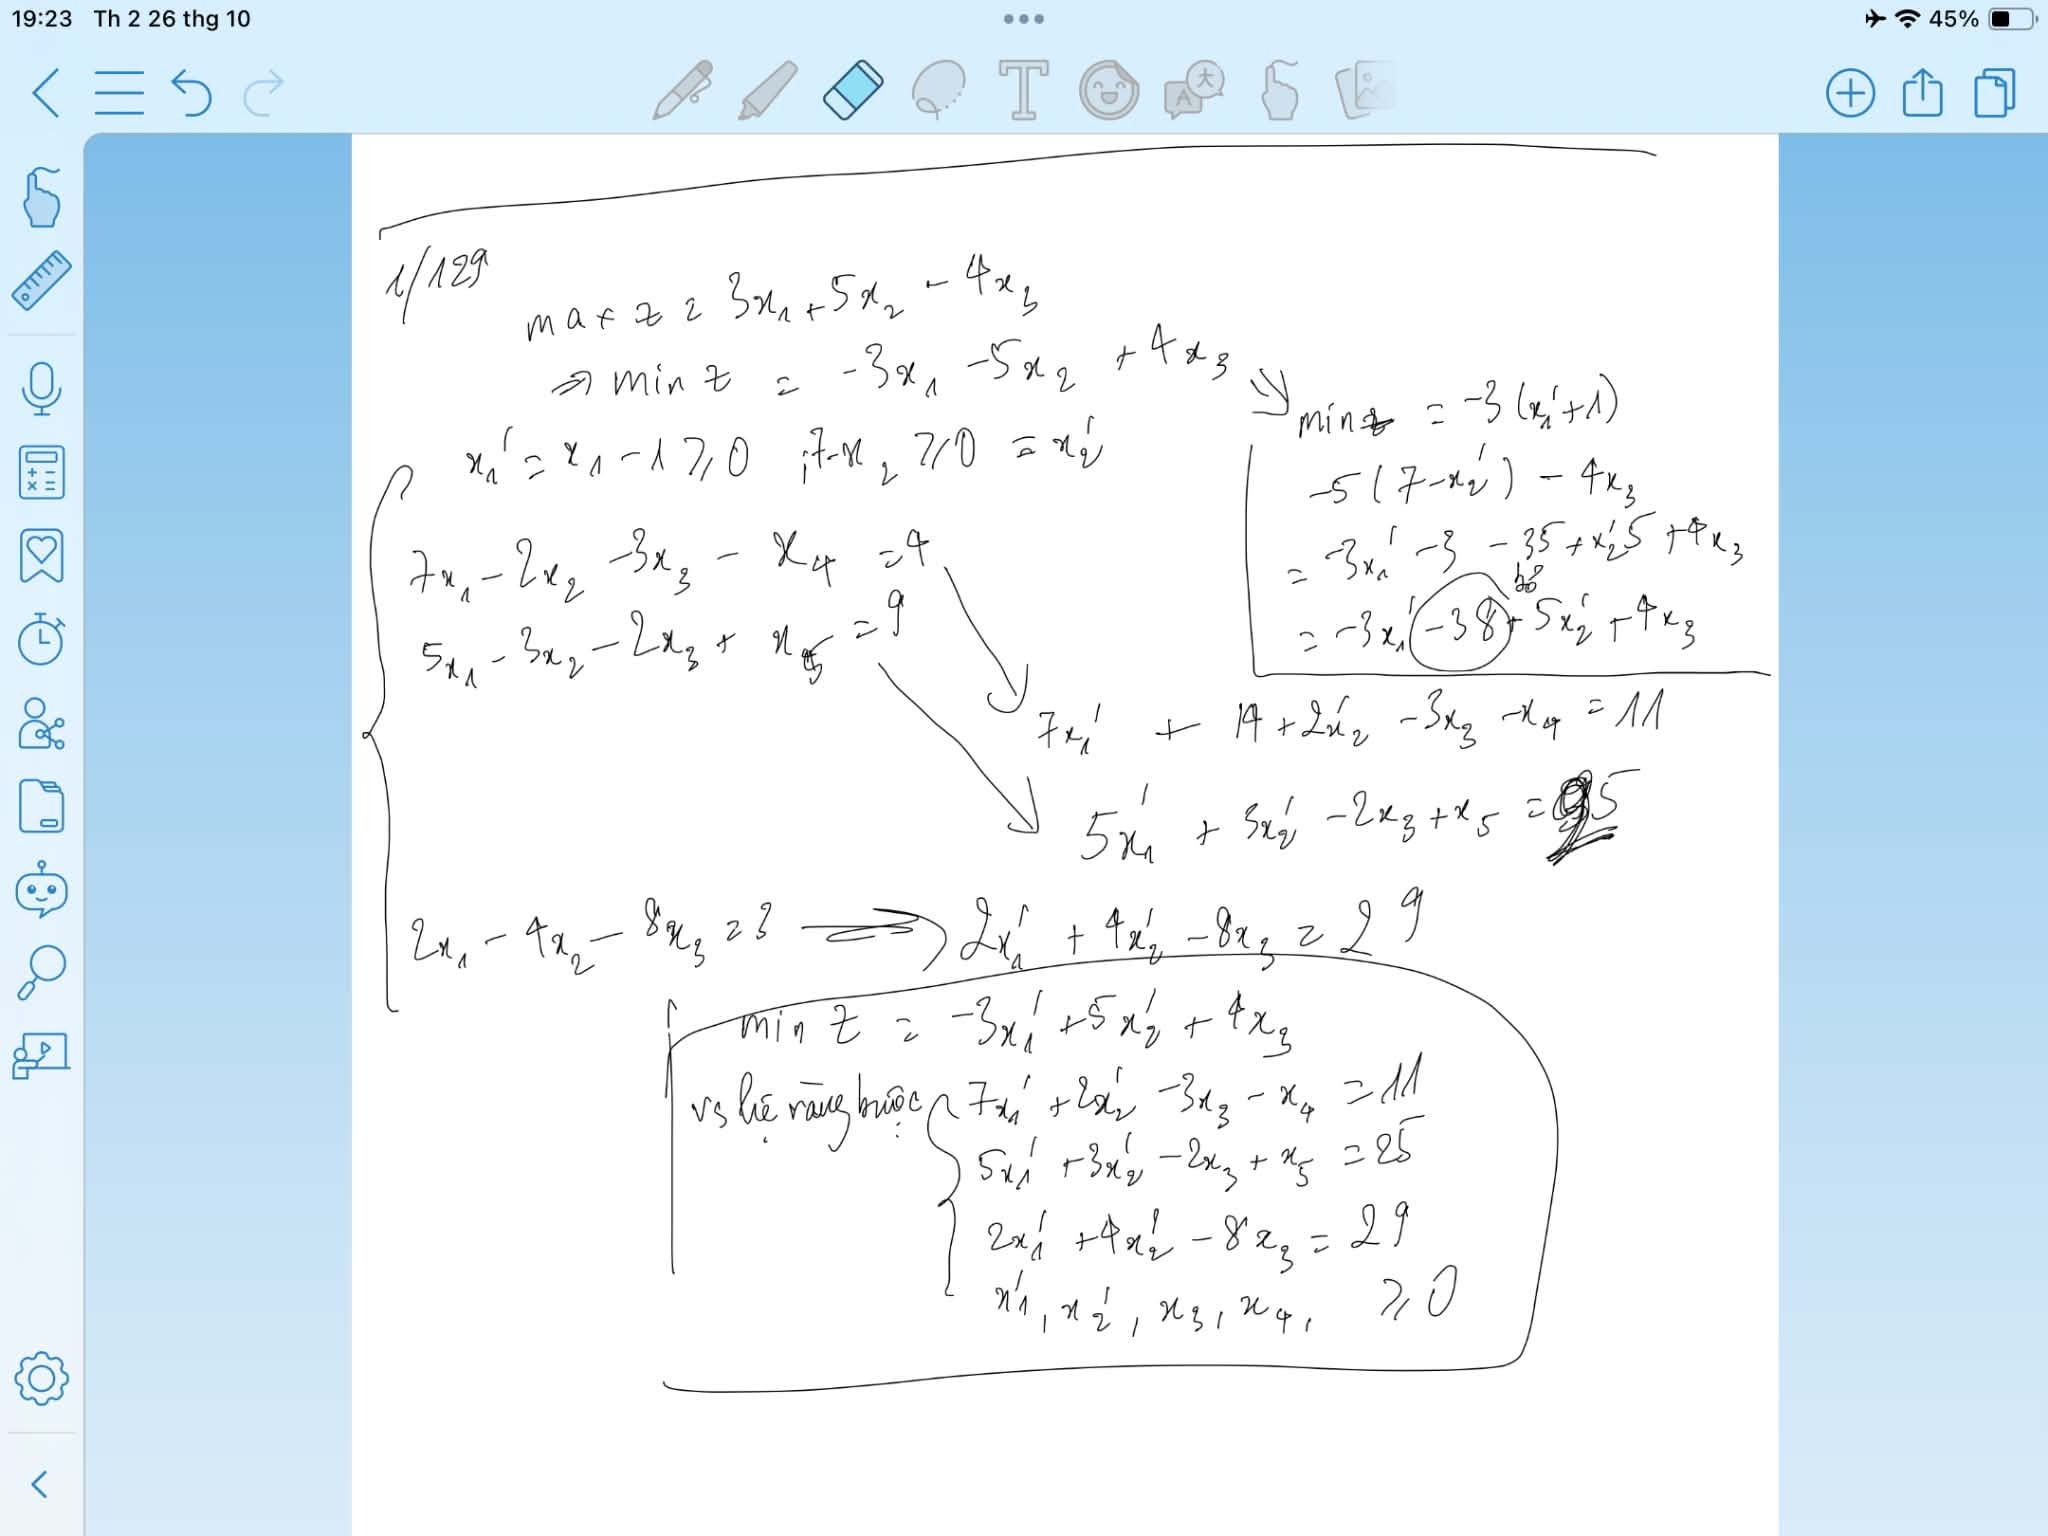
\includegraphics[width=.98\textwidth,height=.82\textheight,keepaspectratio]{bai_lam_them_1_assets/page-035.jpg}\end{center}
\clearpage
\phantomsection\label{src:036}
\noindent\textbf{Ảnh nguồn 036}\par\medskip
\begin{center}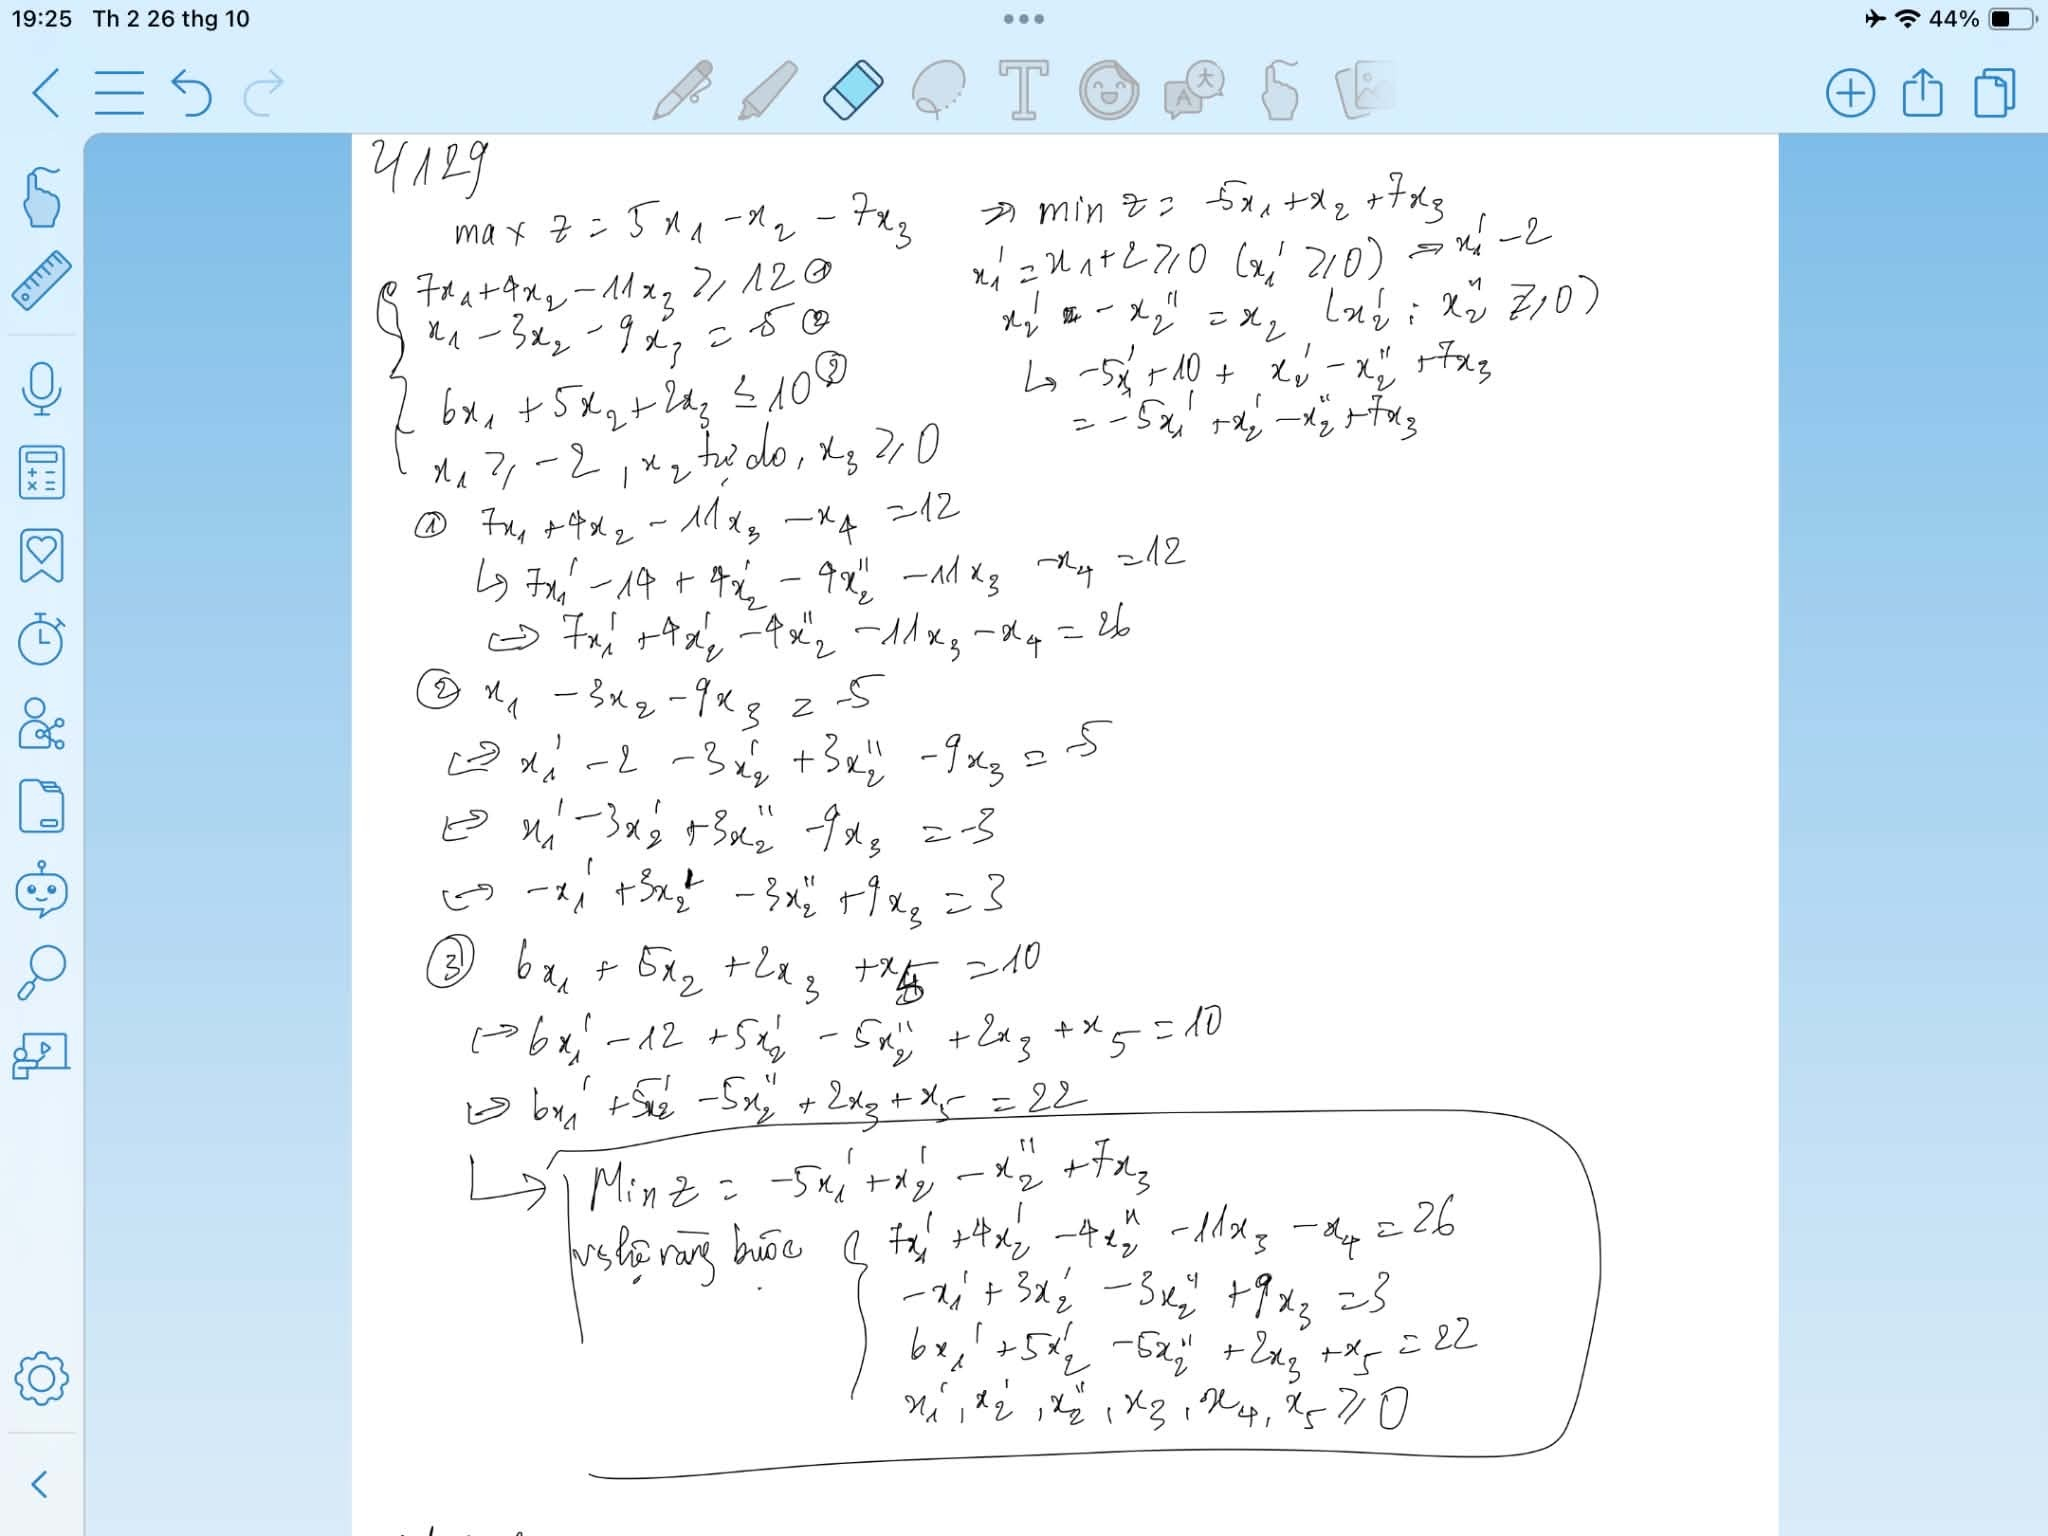
\includegraphics[width=.98\textwidth,height=.82\textheight,keepaspectratio]{bai_lam_them_1_assets/page-036.jpg}\end{center}
\clearpage
\phantomsection\label{src:037}
\noindent\textbf{Ảnh nguồn 037}\par\medskip
\begin{center}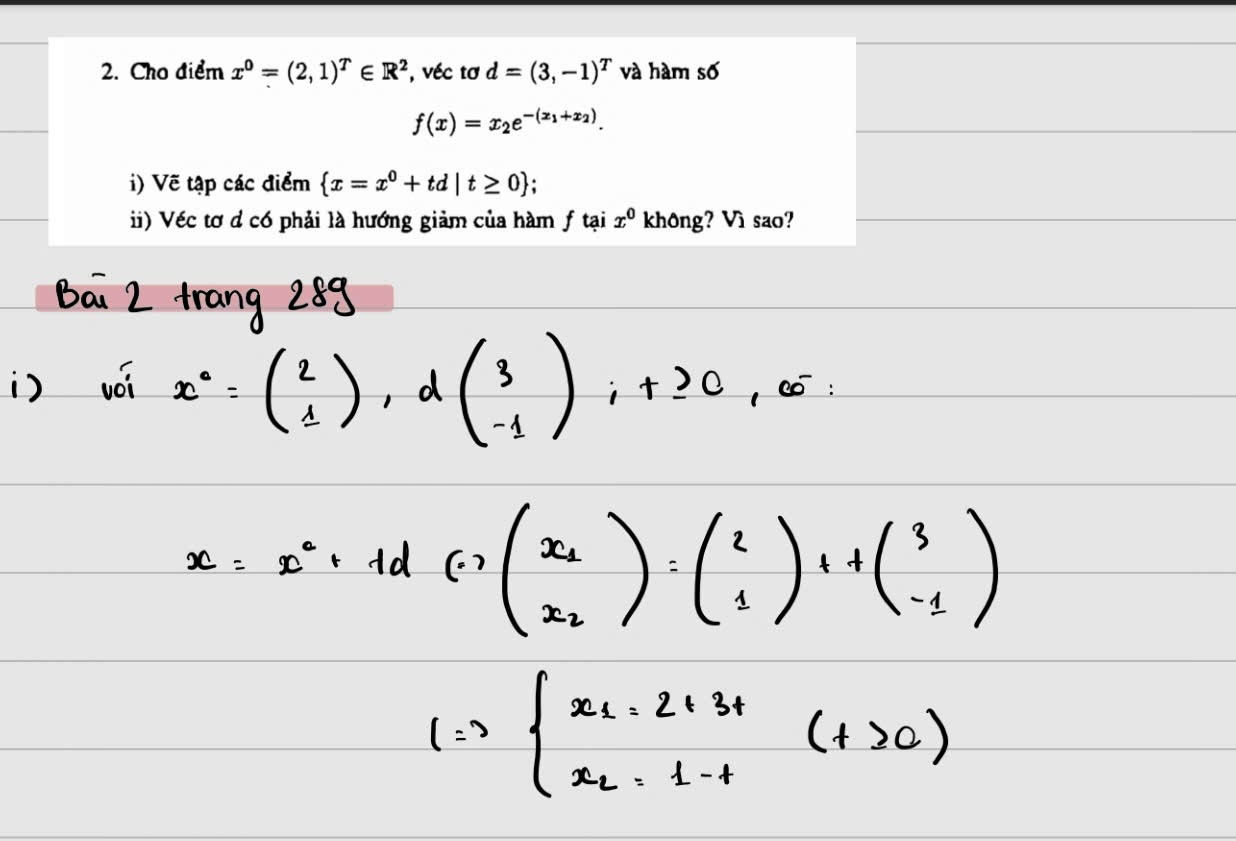
\includegraphics[width=.98\textwidth,height=.82\textheight,keepaspectratio]{bai_lam_them_1_assets/page-037.jpg}\end{center}
\clearpage
\phantomsection\label{src:038}
\noindent\textbf{Ảnh nguồn 038}\par\medskip
\begin{center}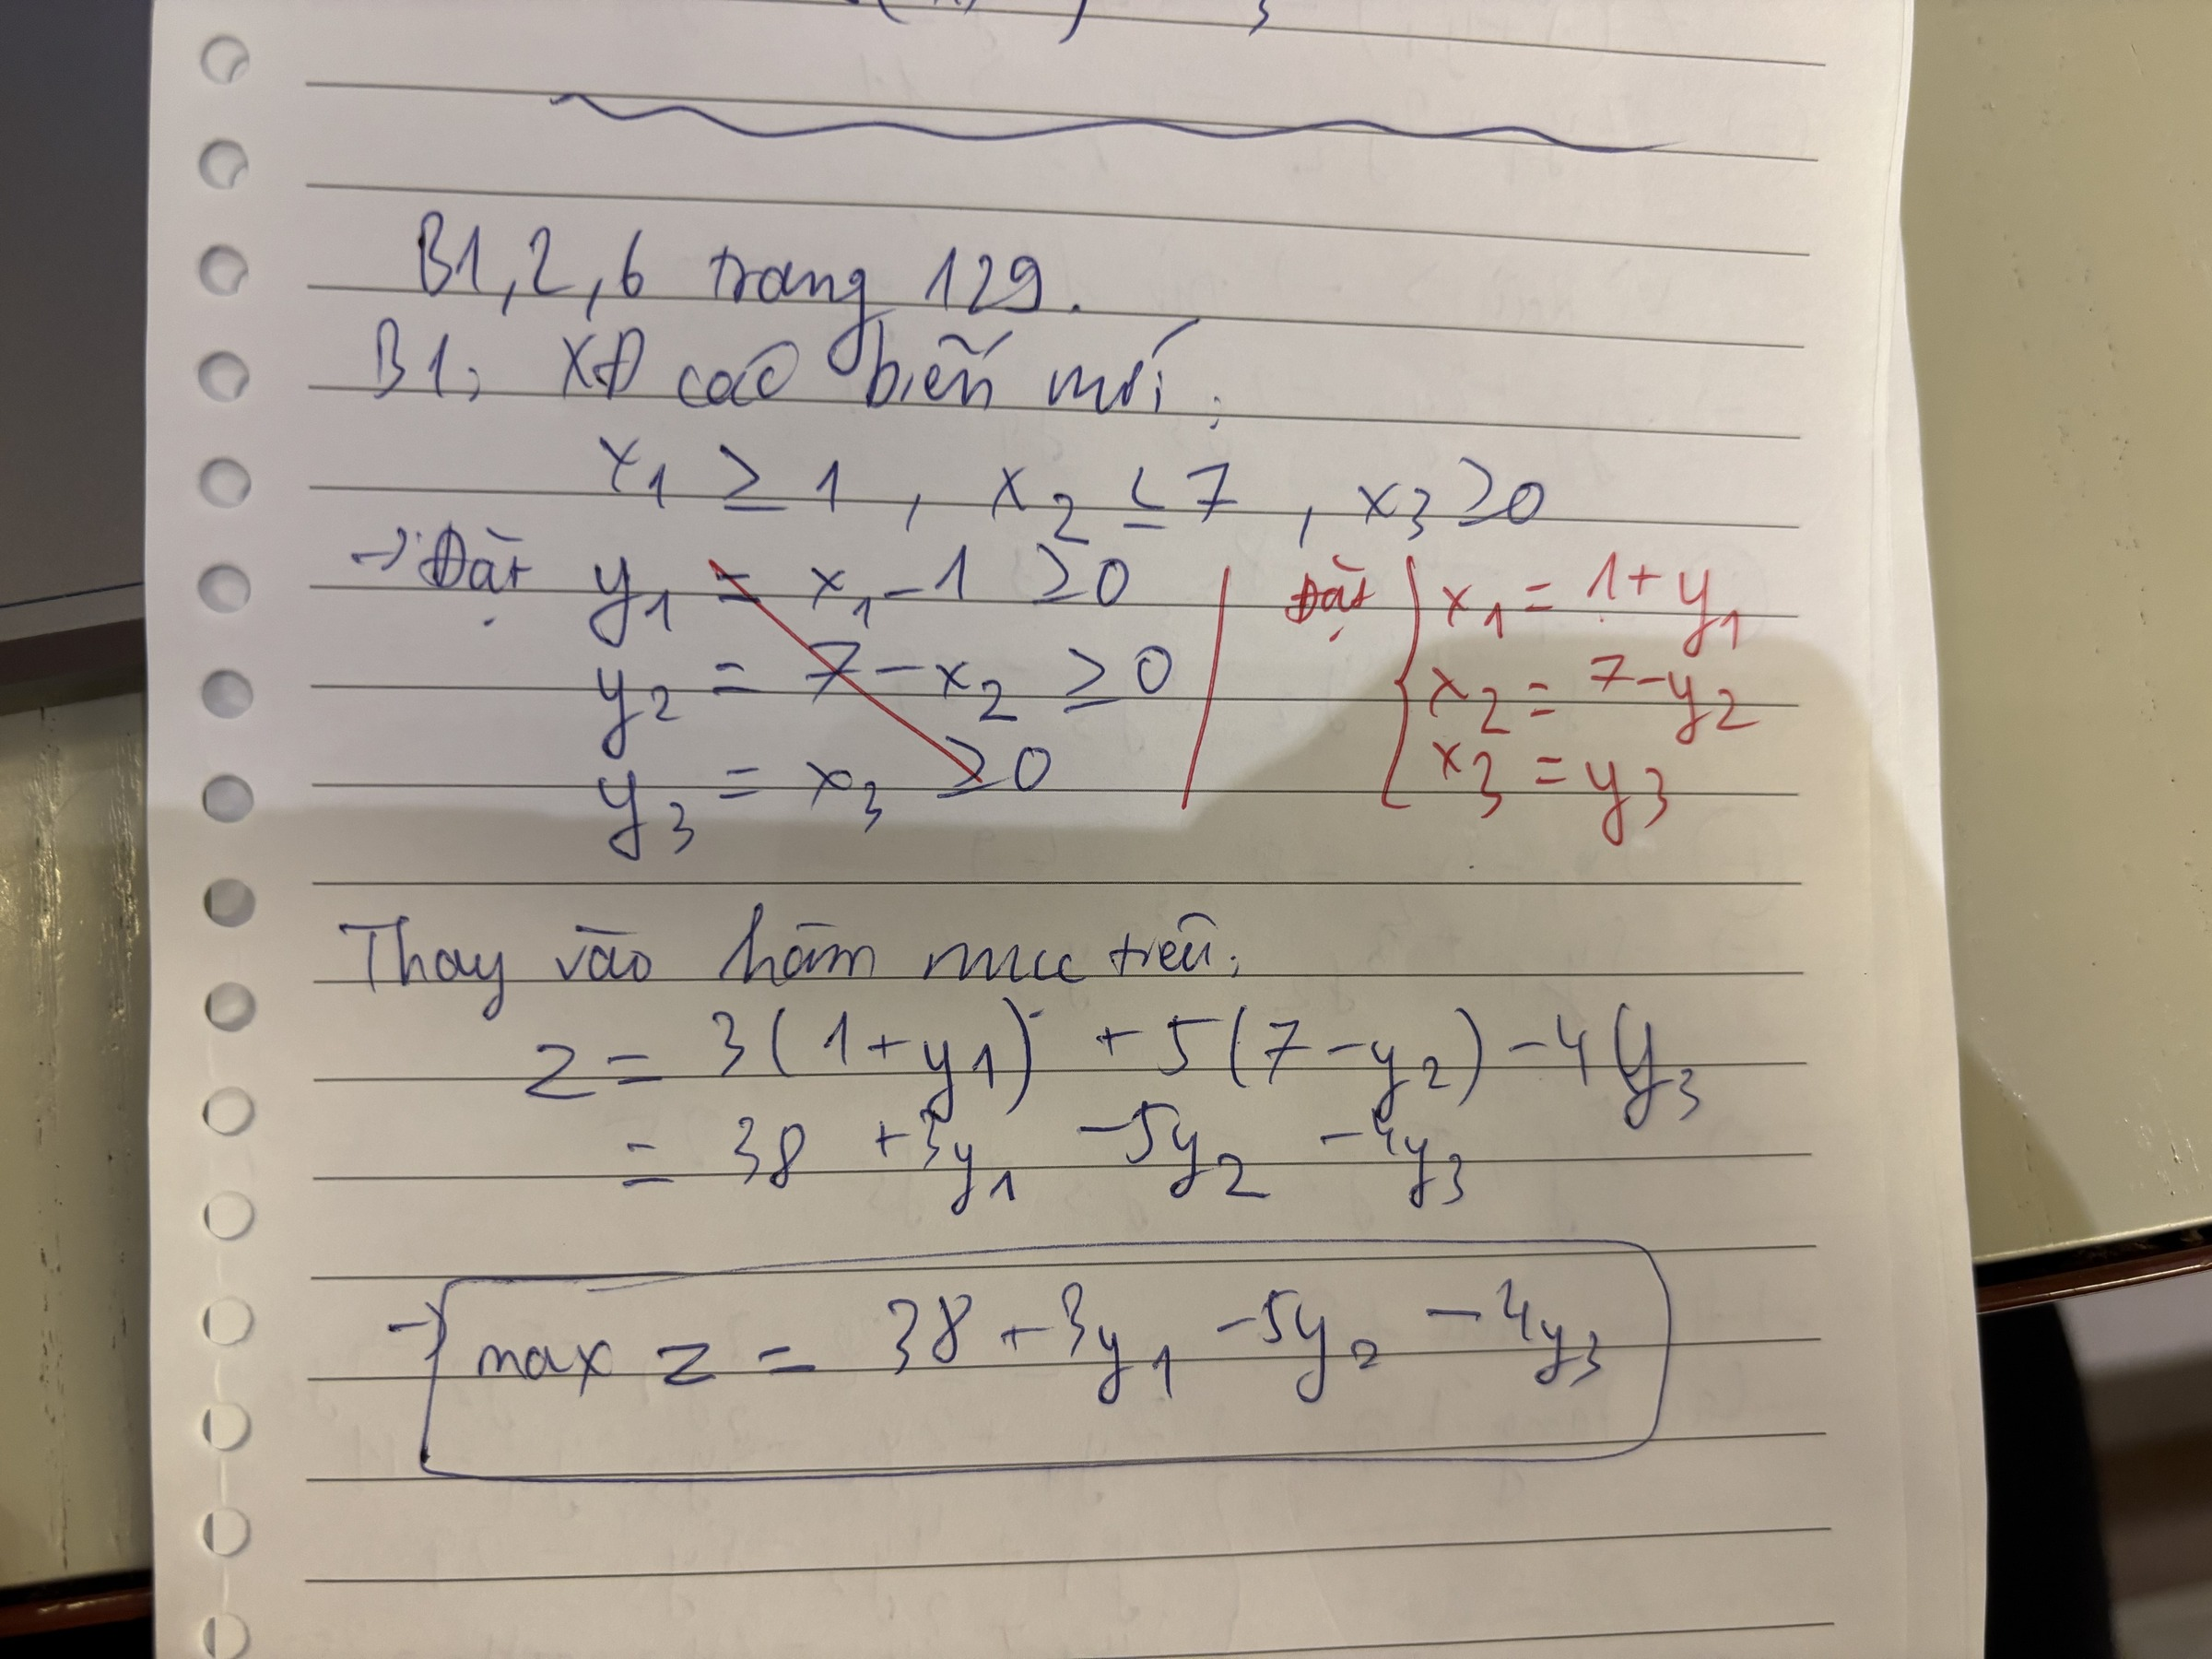
\includegraphics[width=.98\textwidth,height=.82\textheight,keepaspectratio]{bai_lam_them_1_assets/page-038.jpg}\end{center}
\clearpage
\phantomsection\label{src:039}
\noindent\textbf{Ảnh nguồn 039}\par\medskip
\begin{center}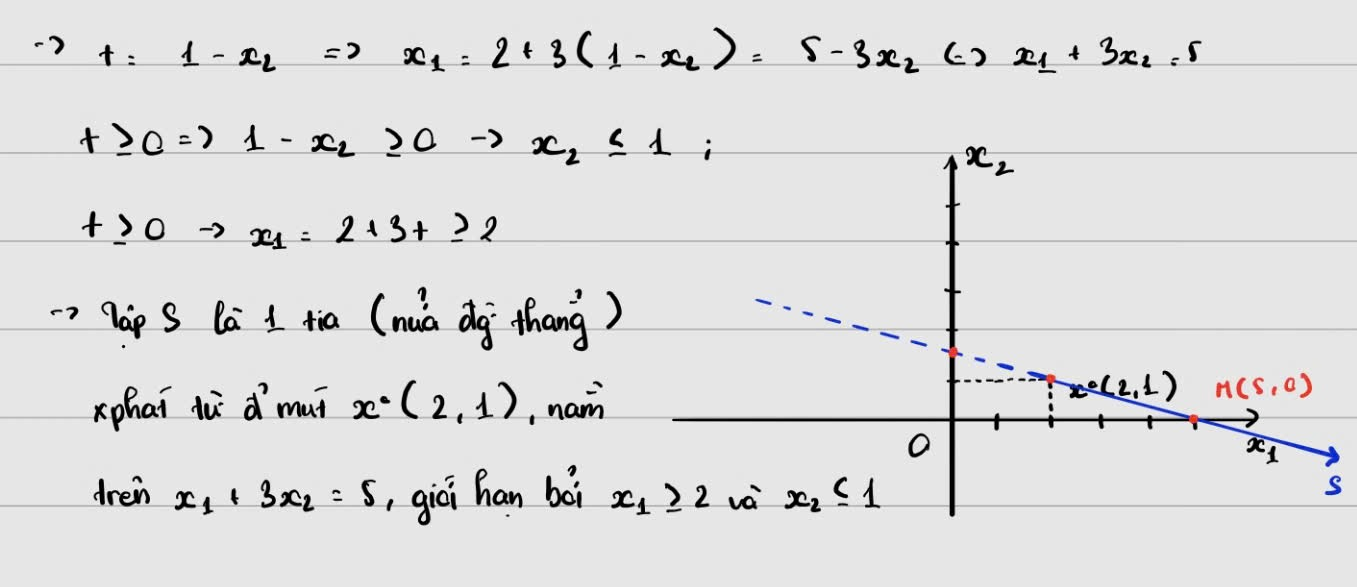
\includegraphics[width=.98\textwidth,height=.82\textheight,keepaspectratio]{bai_lam_them_1_assets/page-039.jpg}\end{center}
\clearpage
\phantomsection\label{src:040}
\noindent\textbf{Ảnh nguồn 040}\par\medskip
\begin{center}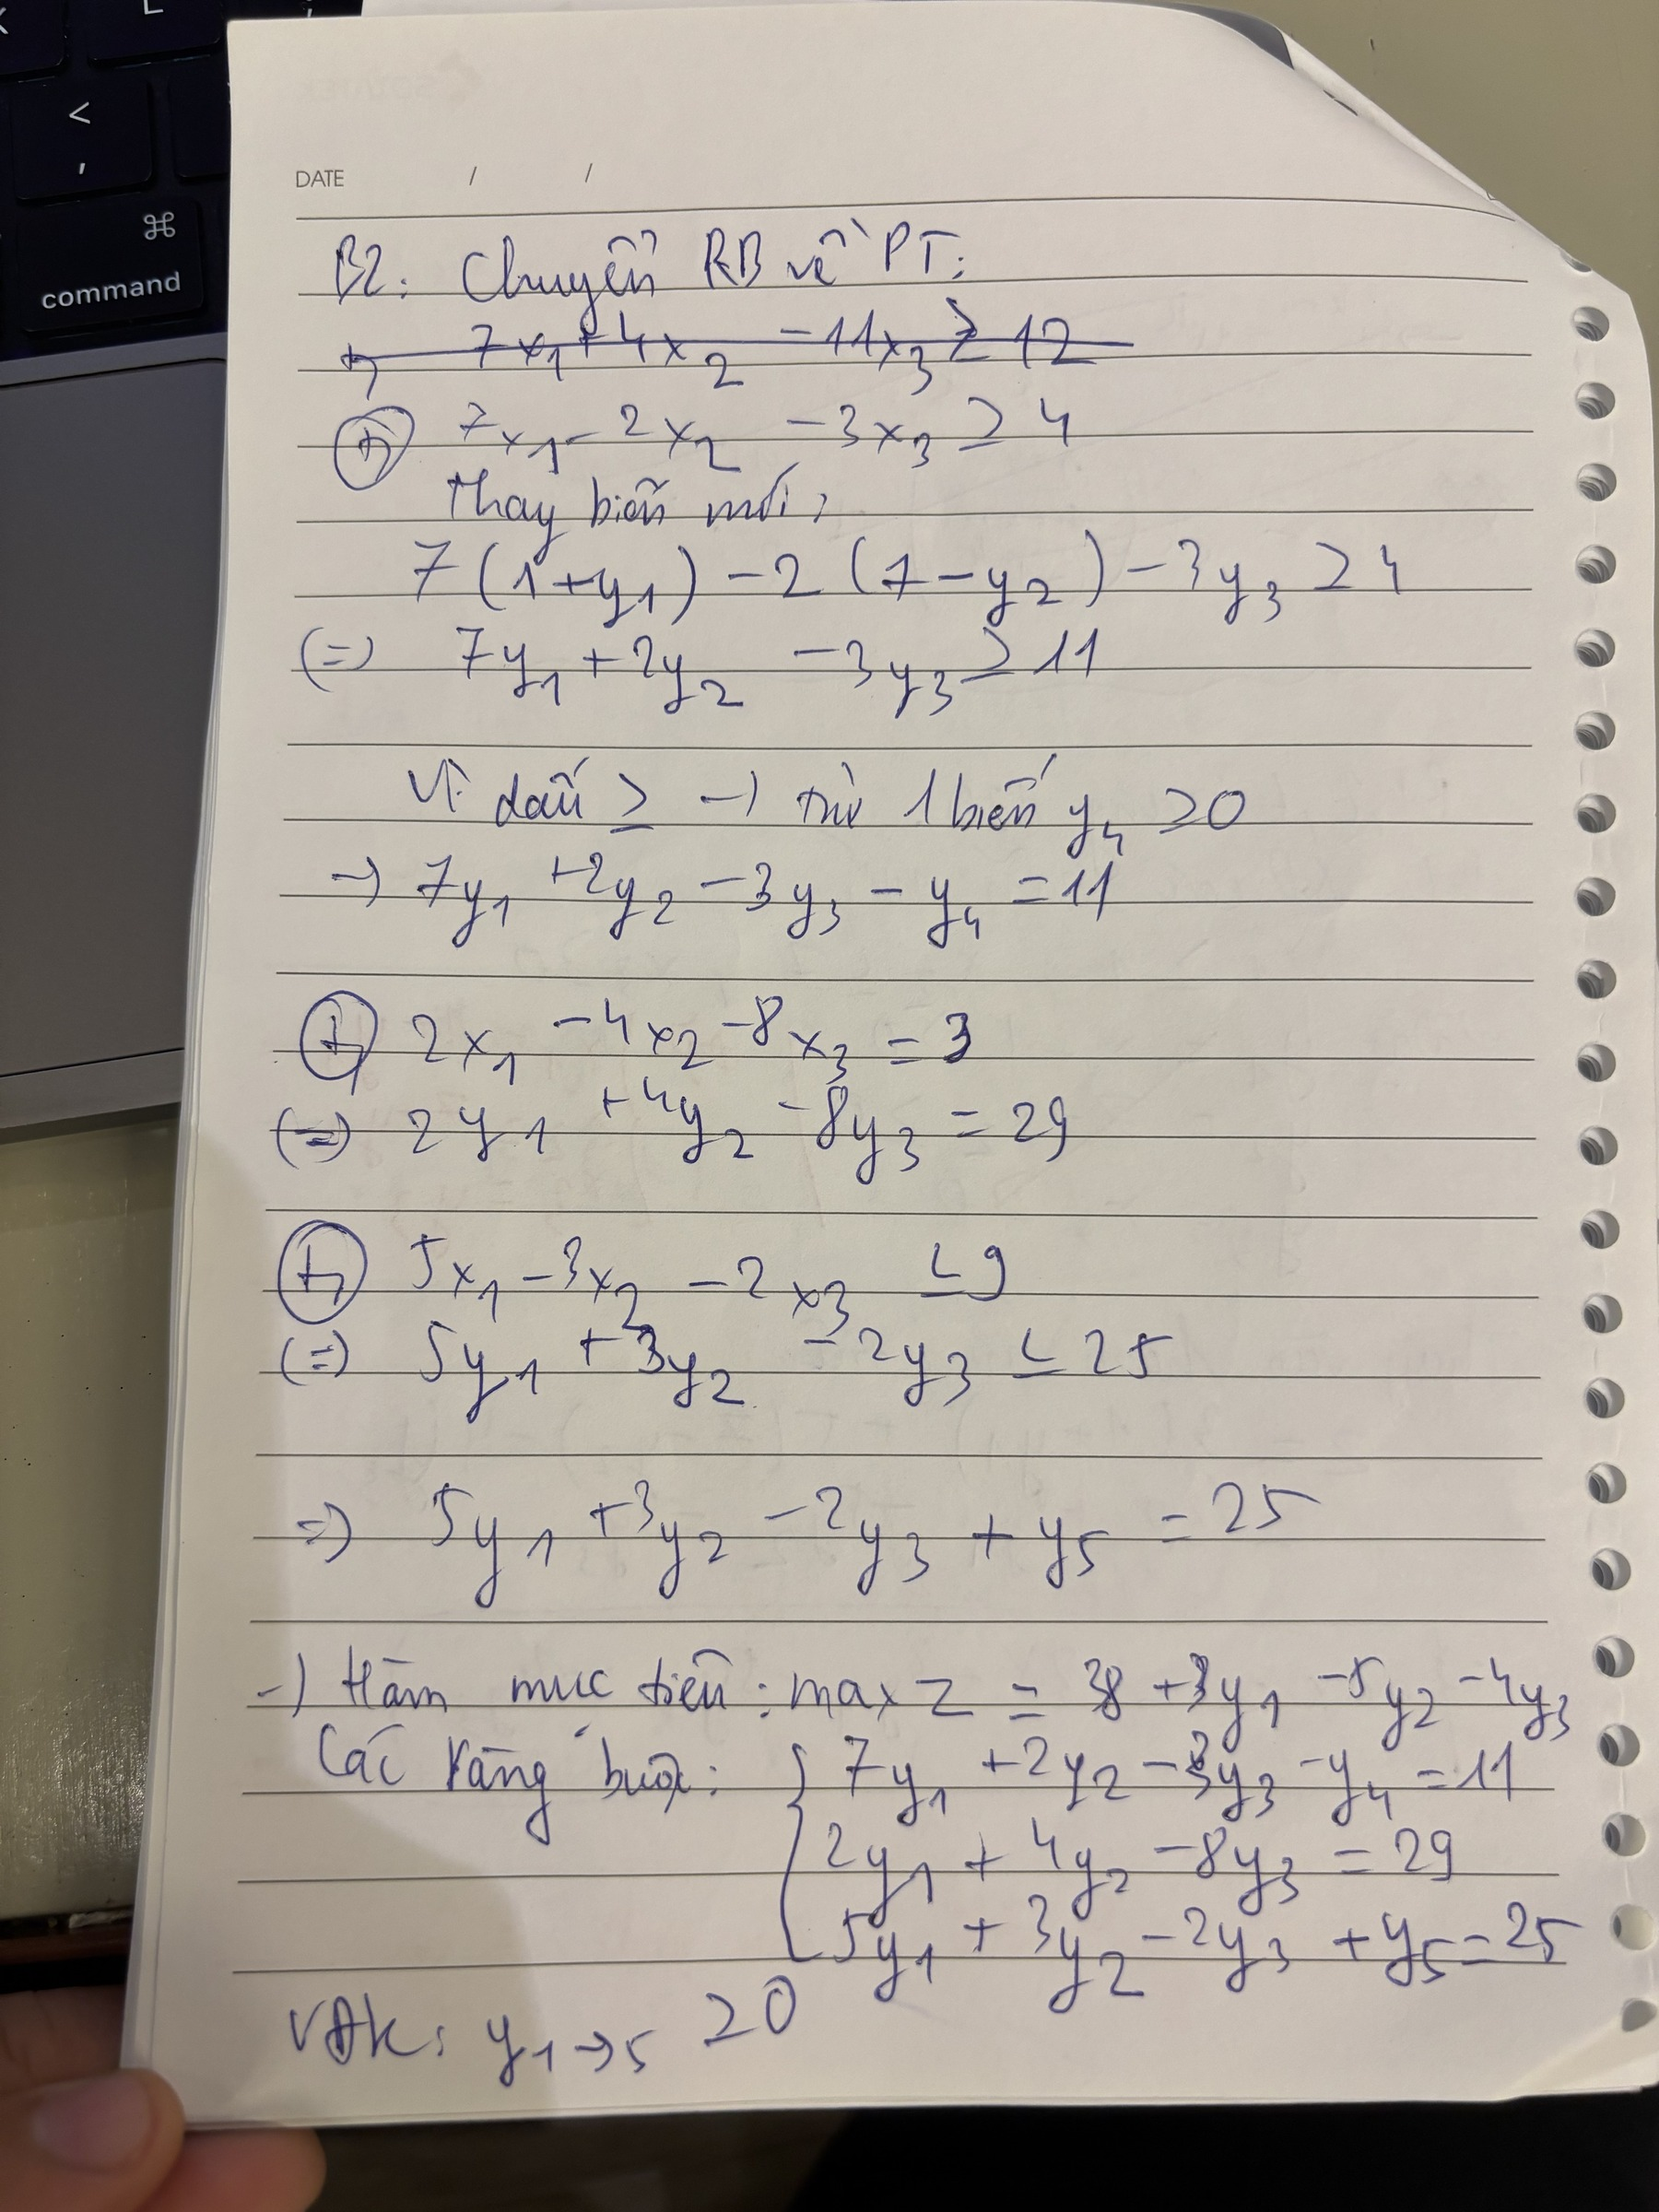
\includegraphics[width=.98\textwidth,height=.82\textheight,keepaspectratio]{bai_lam_them_1_assets/page-040.jpg}\end{center}
\clearpage
\phantomsection\label{src:041}
\noindent\textbf{Ảnh nguồn 041}\par\medskip
\begin{center}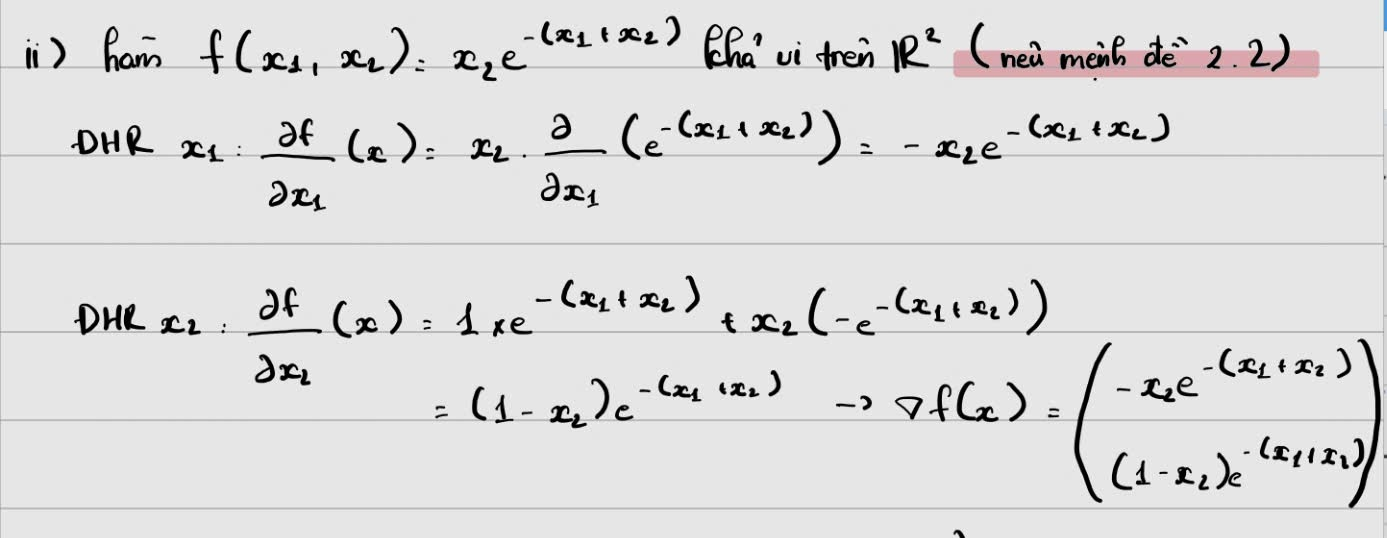
\includegraphics[width=.98\textwidth,height=.82\textheight,keepaspectratio]{bai_lam_them_1_assets/page-041.jpg}\end{center}
\clearpage
\phantomsection\label{src:042}
\noindent\textbf{Ảnh nguồn 042}\par\medskip
\begin{center}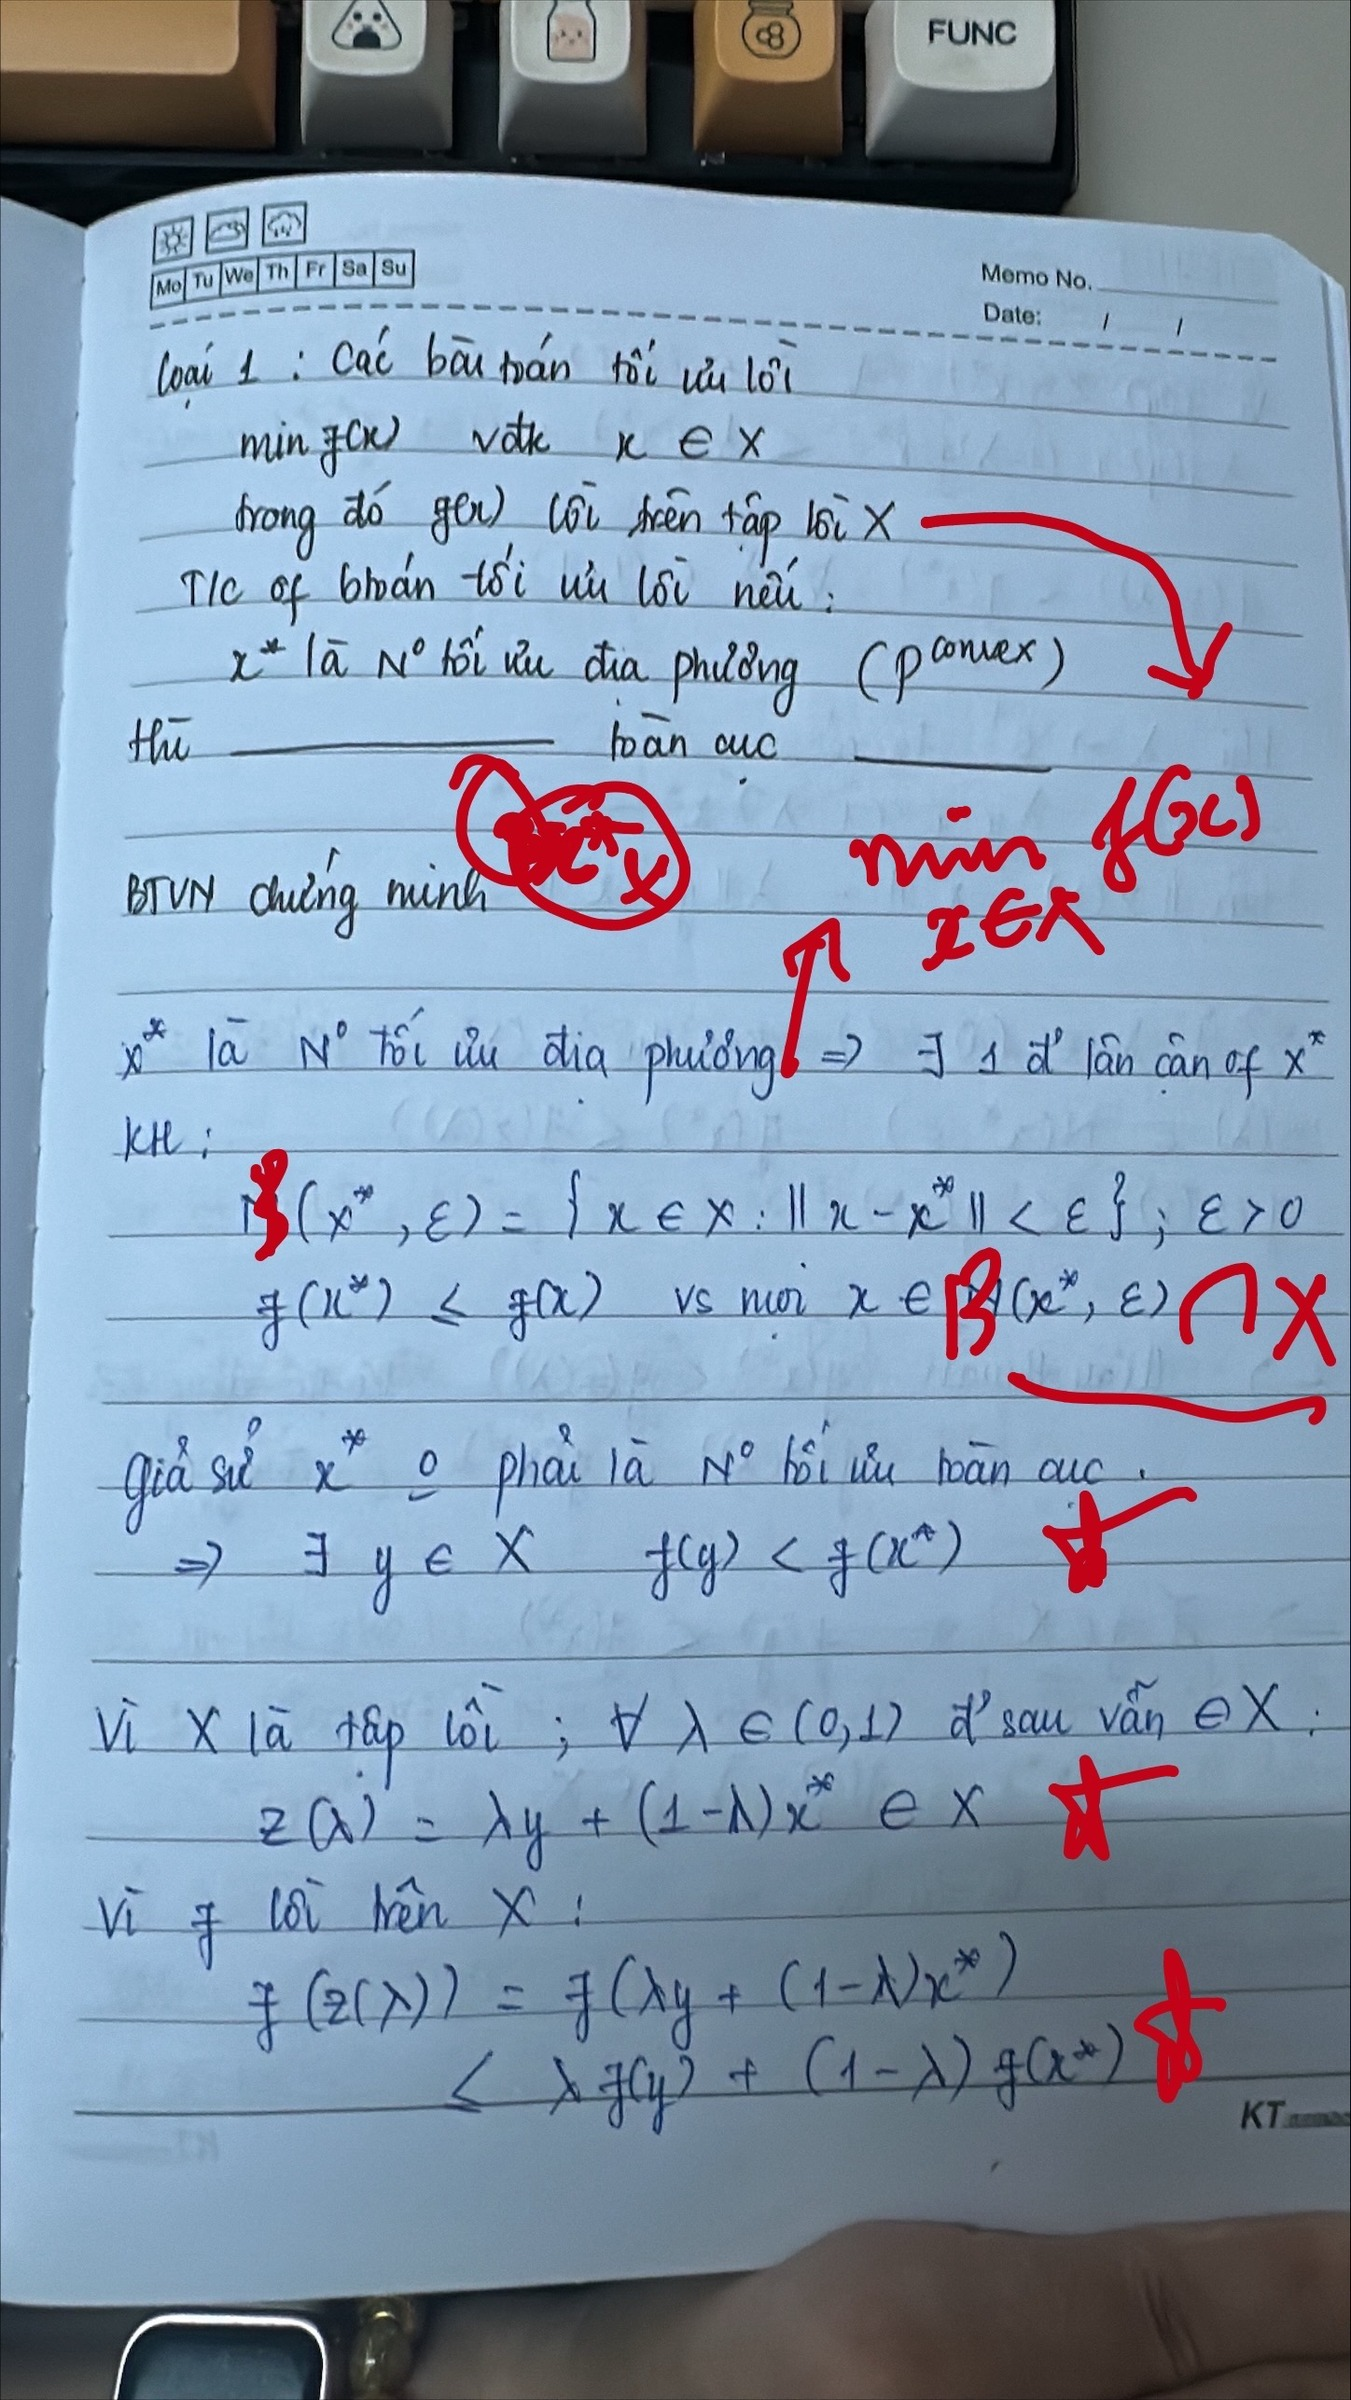
\includegraphics[width=.98\textwidth,height=.82\textheight,keepaspectratio]{bai_lam_them_1_assets/page-042.jpg}\end{center}
\clearpage
\phantomsection\label{src:043}
\noindent\textbf{Ảnh nguồn 043}\par\medskip
\begin{center}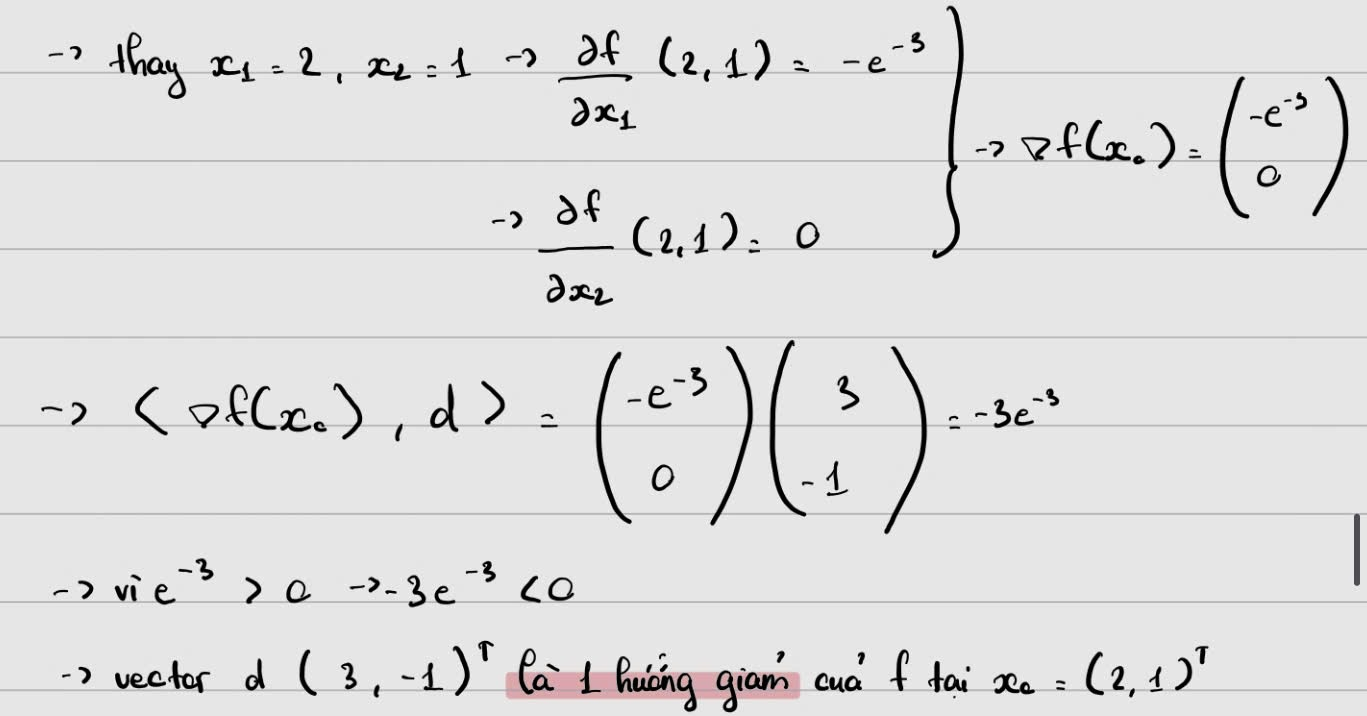
\includegraphics[width=.98\textwidth,height=.82\textheight,keepaspectratio]{bai_lam_them_1_assets/page-043.jpg}\end{center}
\clearpage
\phantomsection\label{src:044}
\noindent\textbf{Ảnh nguồn 044}\par\medskip
\begin{center}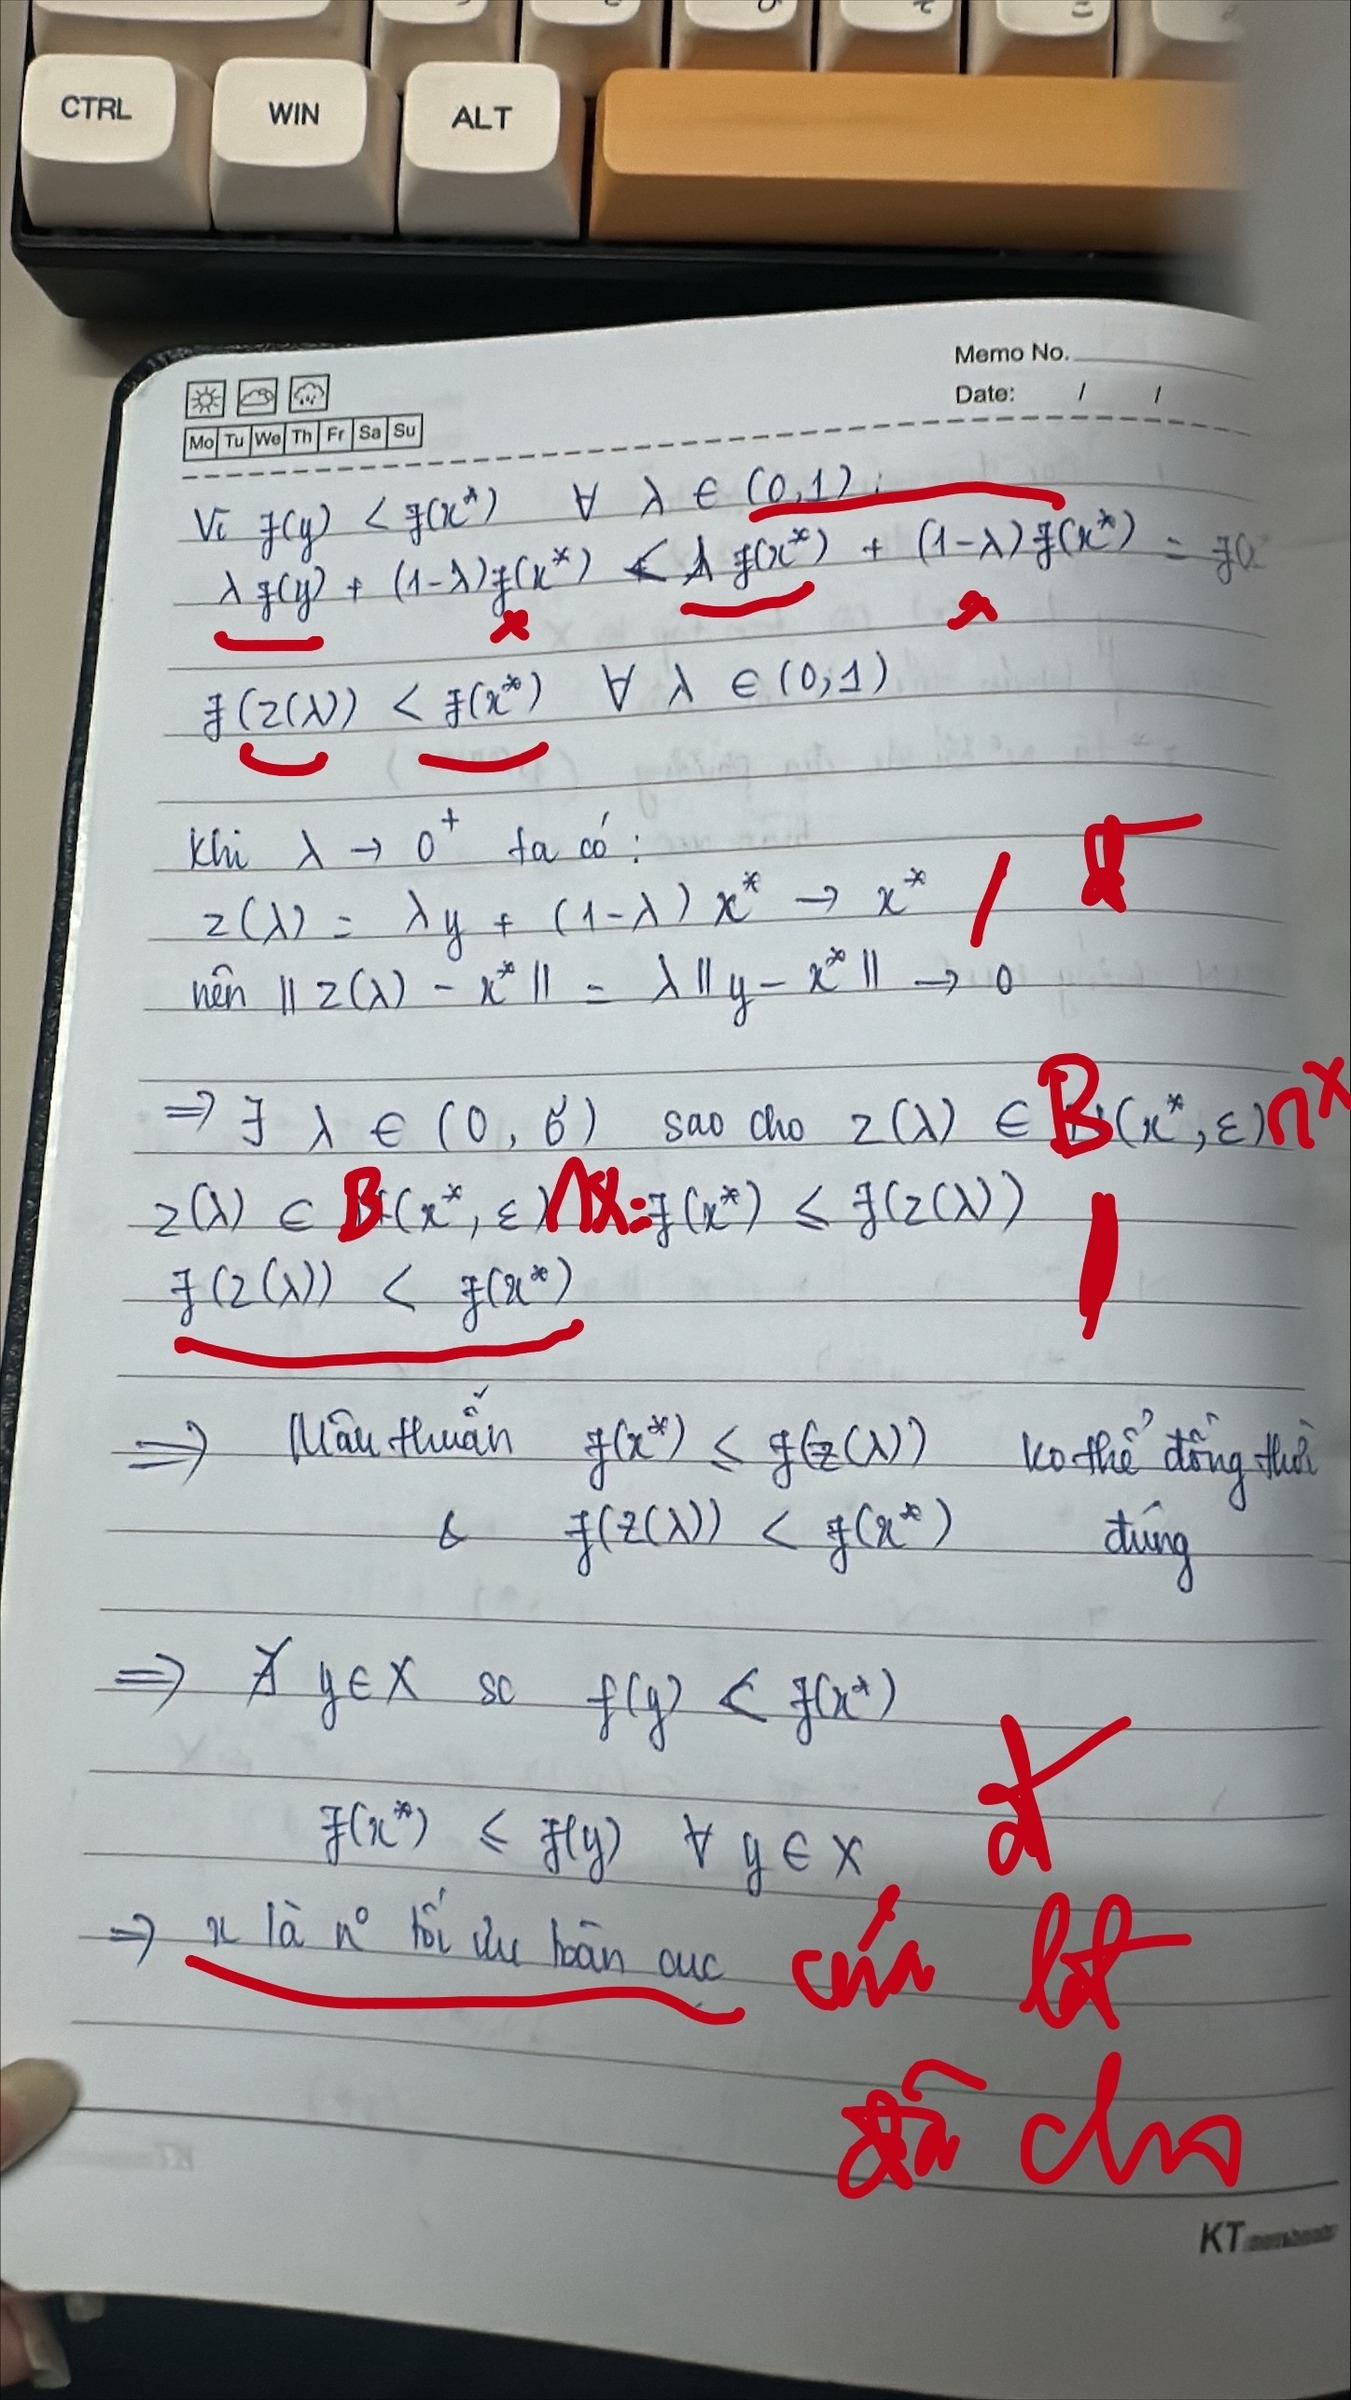
\includegraphics[width=.98\textwidth,height=.82\textheight,keepaspectratio]{bai_lam_them_1_assets/page-044.jpg}\end{center}
\clearpage
\phantomsection\label{src:045}
\noindent\textbf{Ảnh nguồn 045}\par\medskip
\begin{center}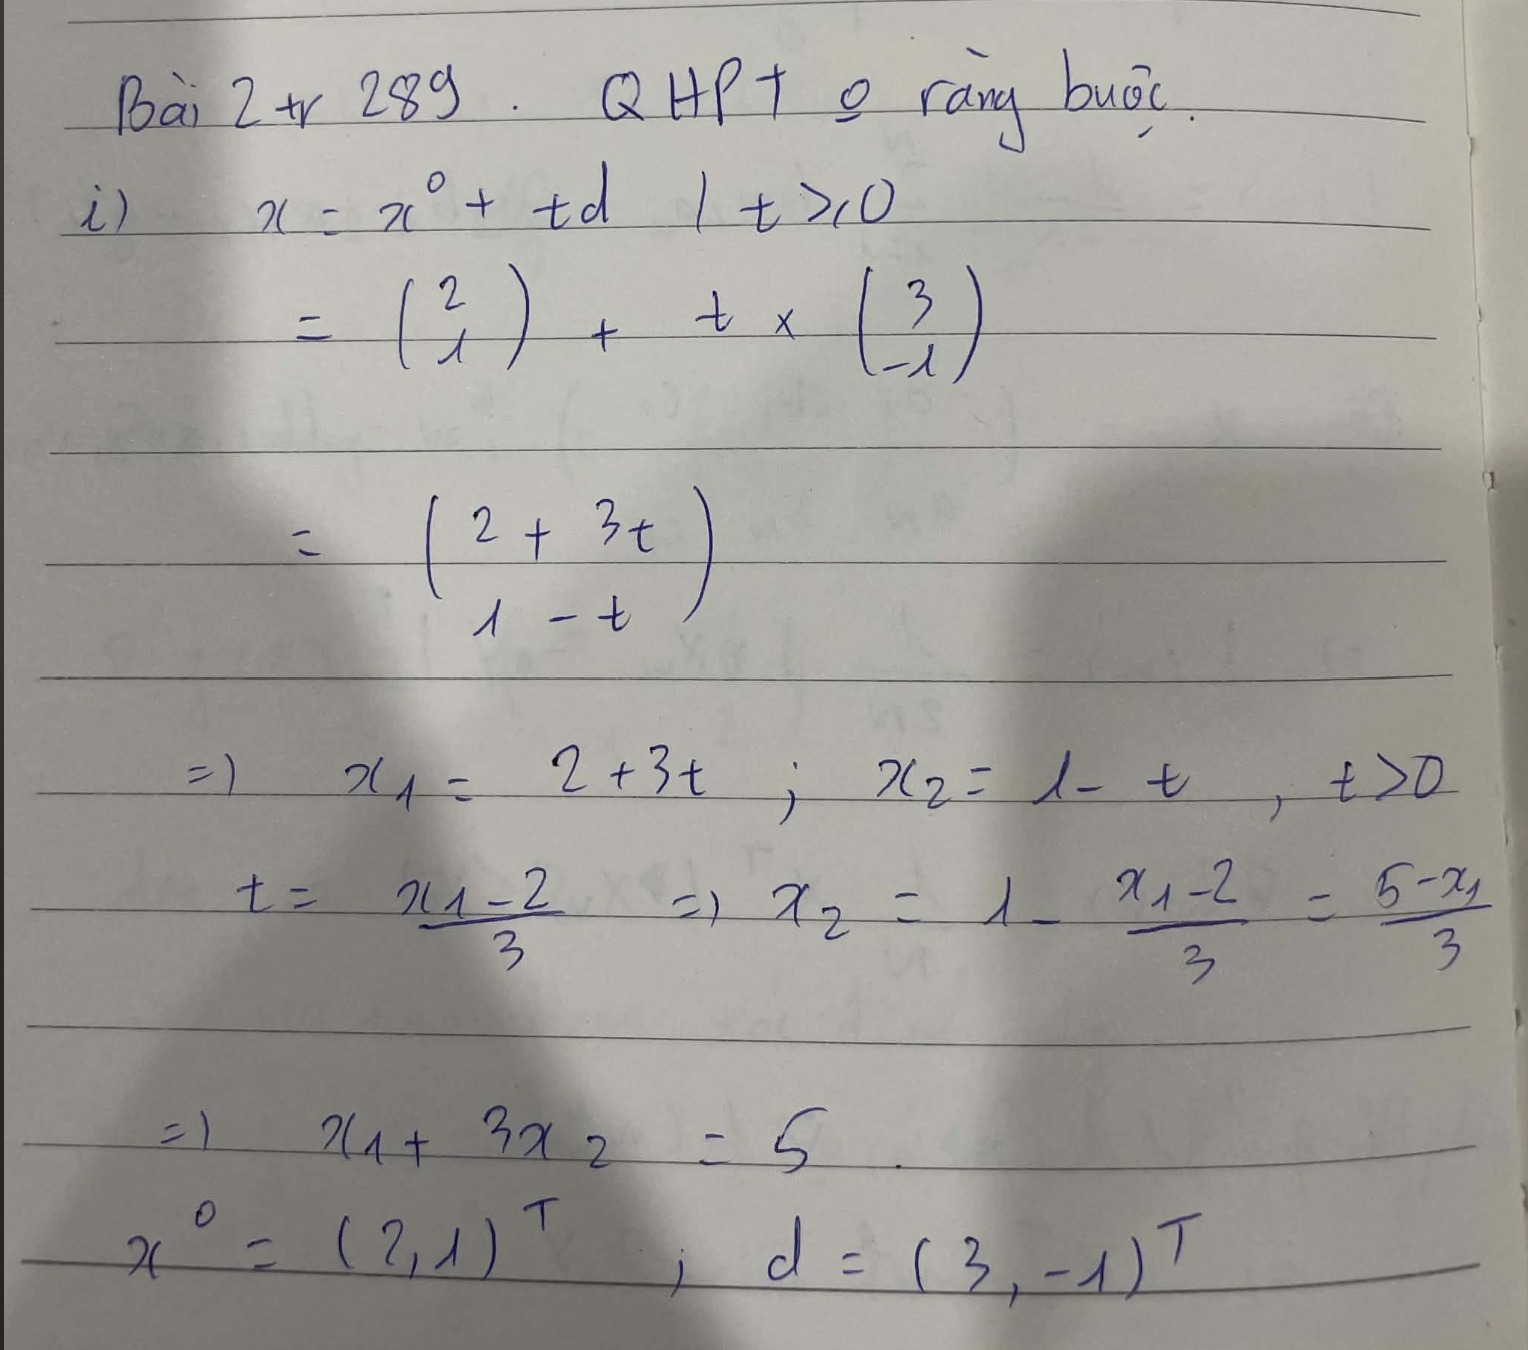
\includegraphics[width=.98\textwidth,height=.82\textheight,keepaspectratio]{bai_lam_them_1_assets/page-045.jpg}\end{center}
\clearpage
\phantomsection\label{src:046}
\noindent\textbf{Ảnh nguồn 046}\par\medskip
\begin{center}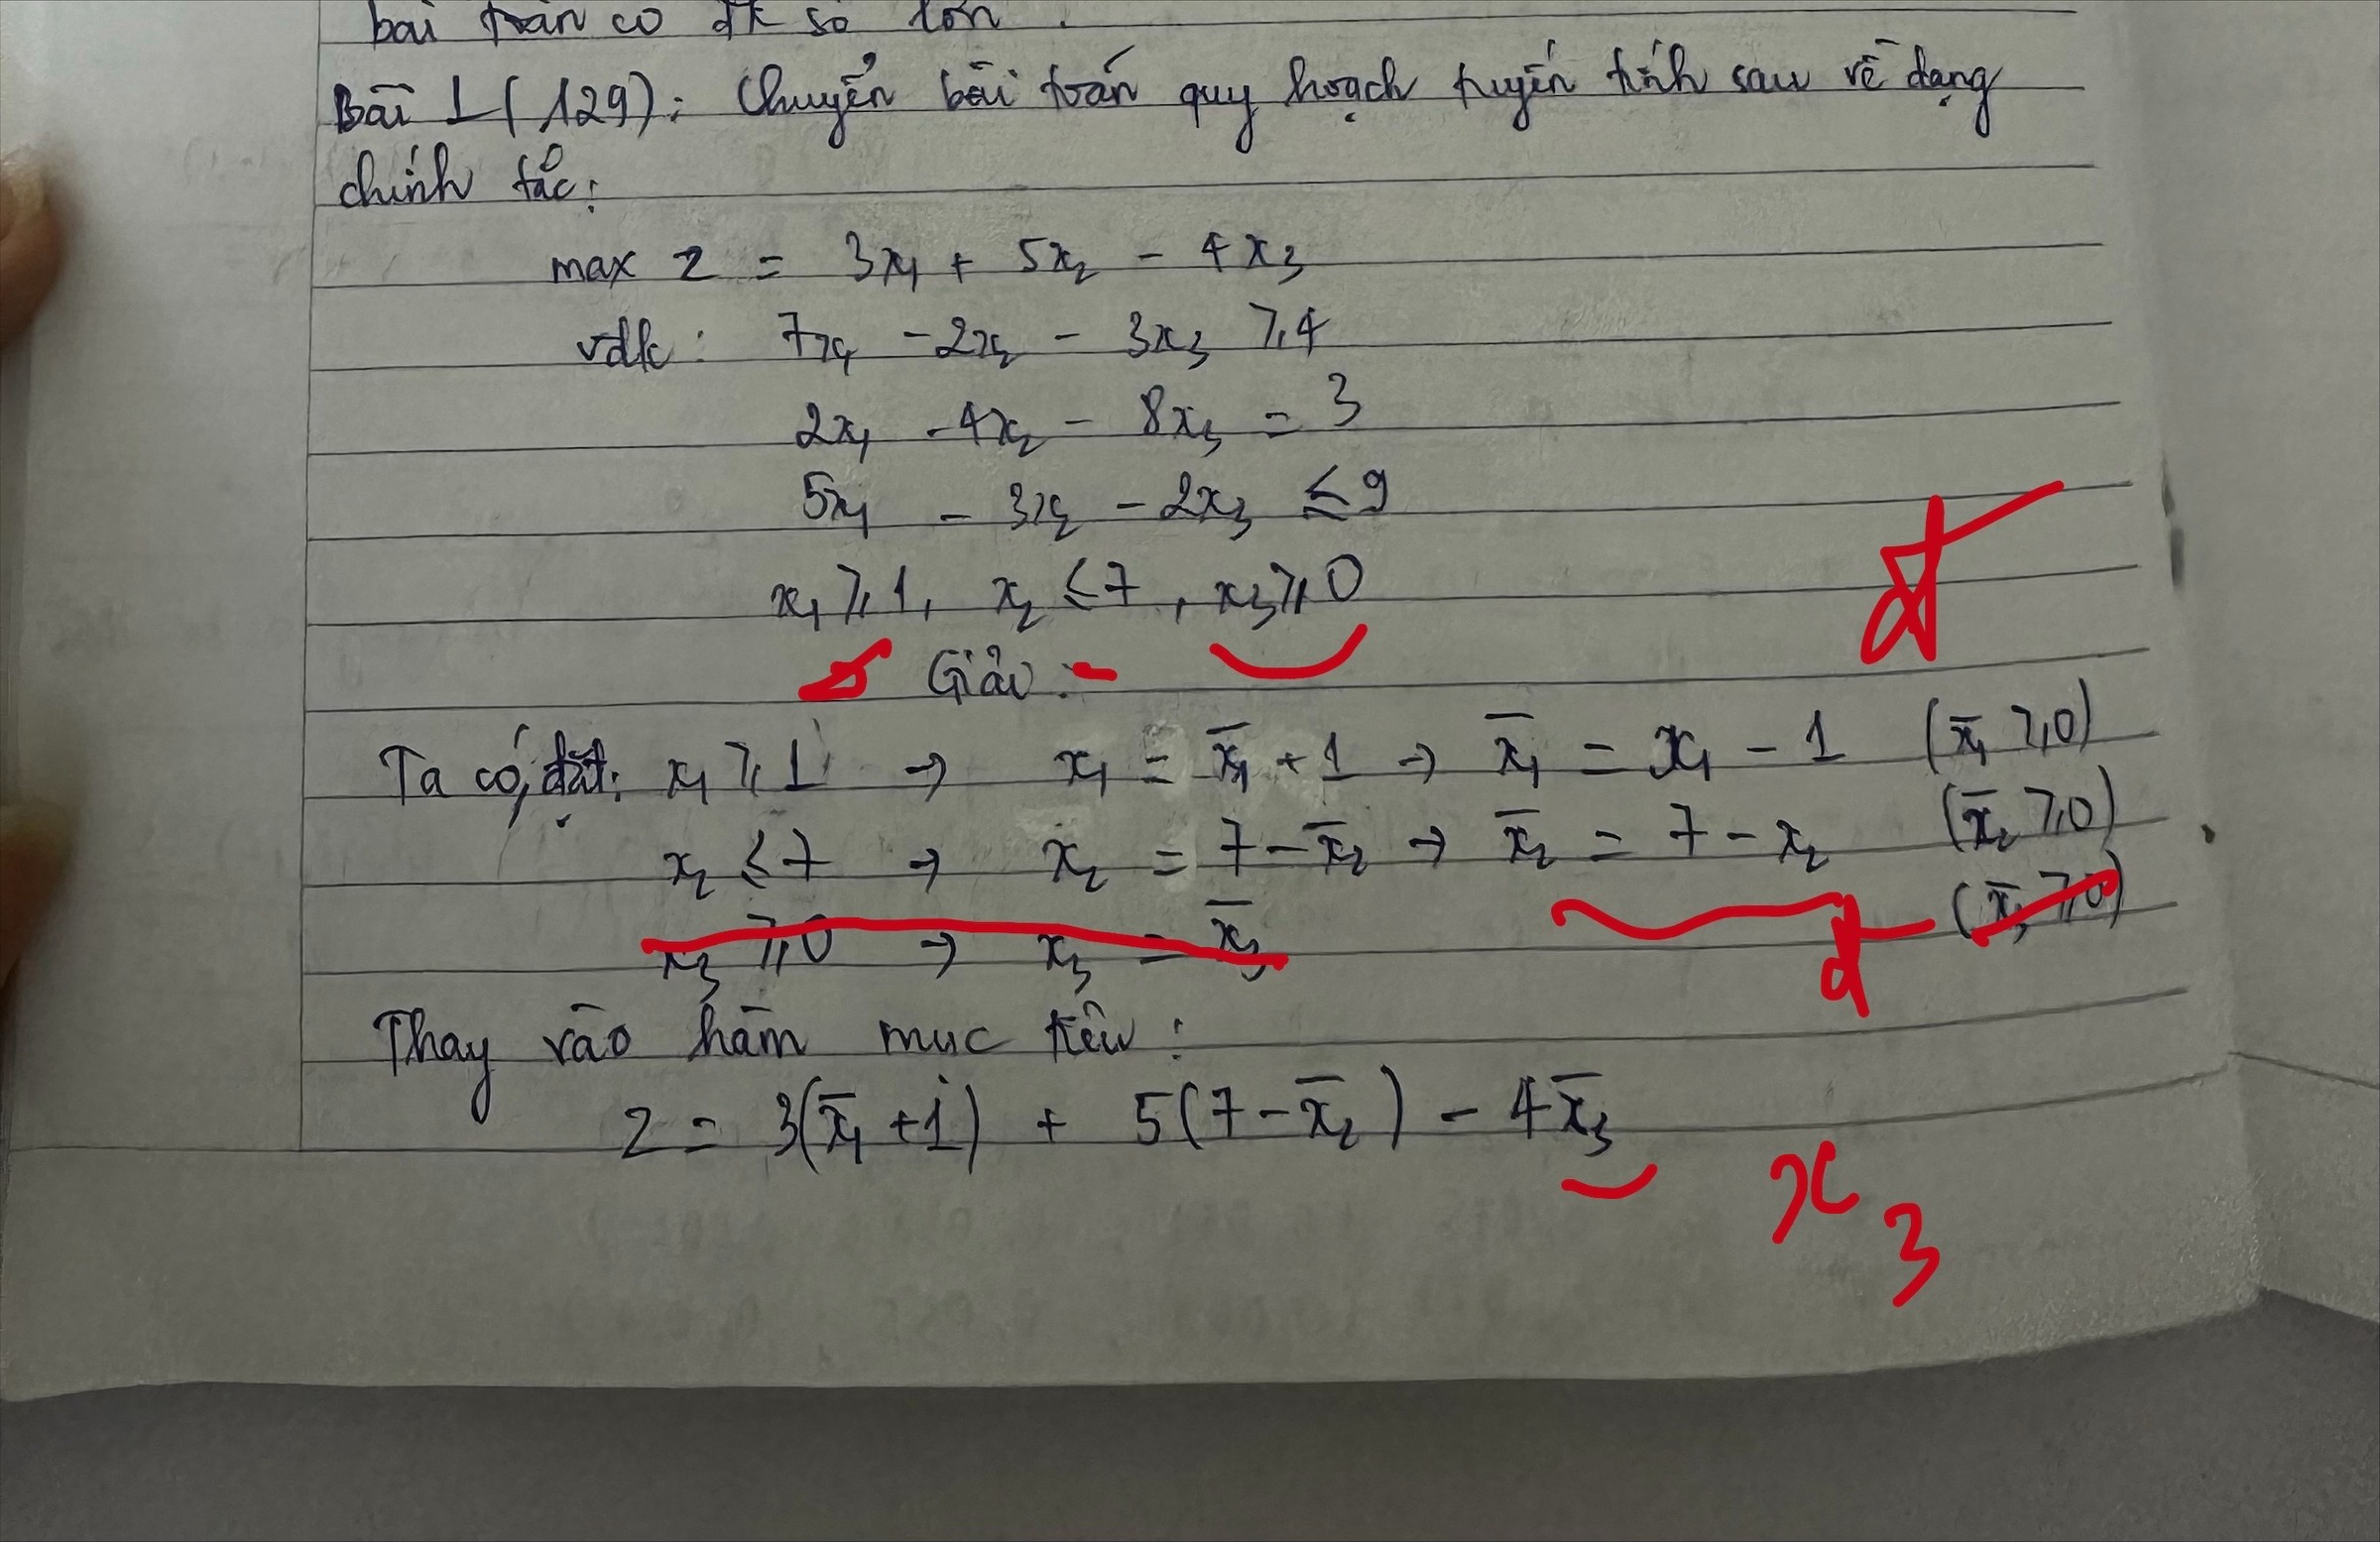
\includegraphics[width=.98\textwidth,height=.82\textheight,keepaspectratio]{bai_lam_them_1_assets/page-046.jpg}\end{center}
\clearpage
\phantomsection\label{src:047}
\noindent\textbf{Ảnh nguồn 047}\par\medskip
\begin{center}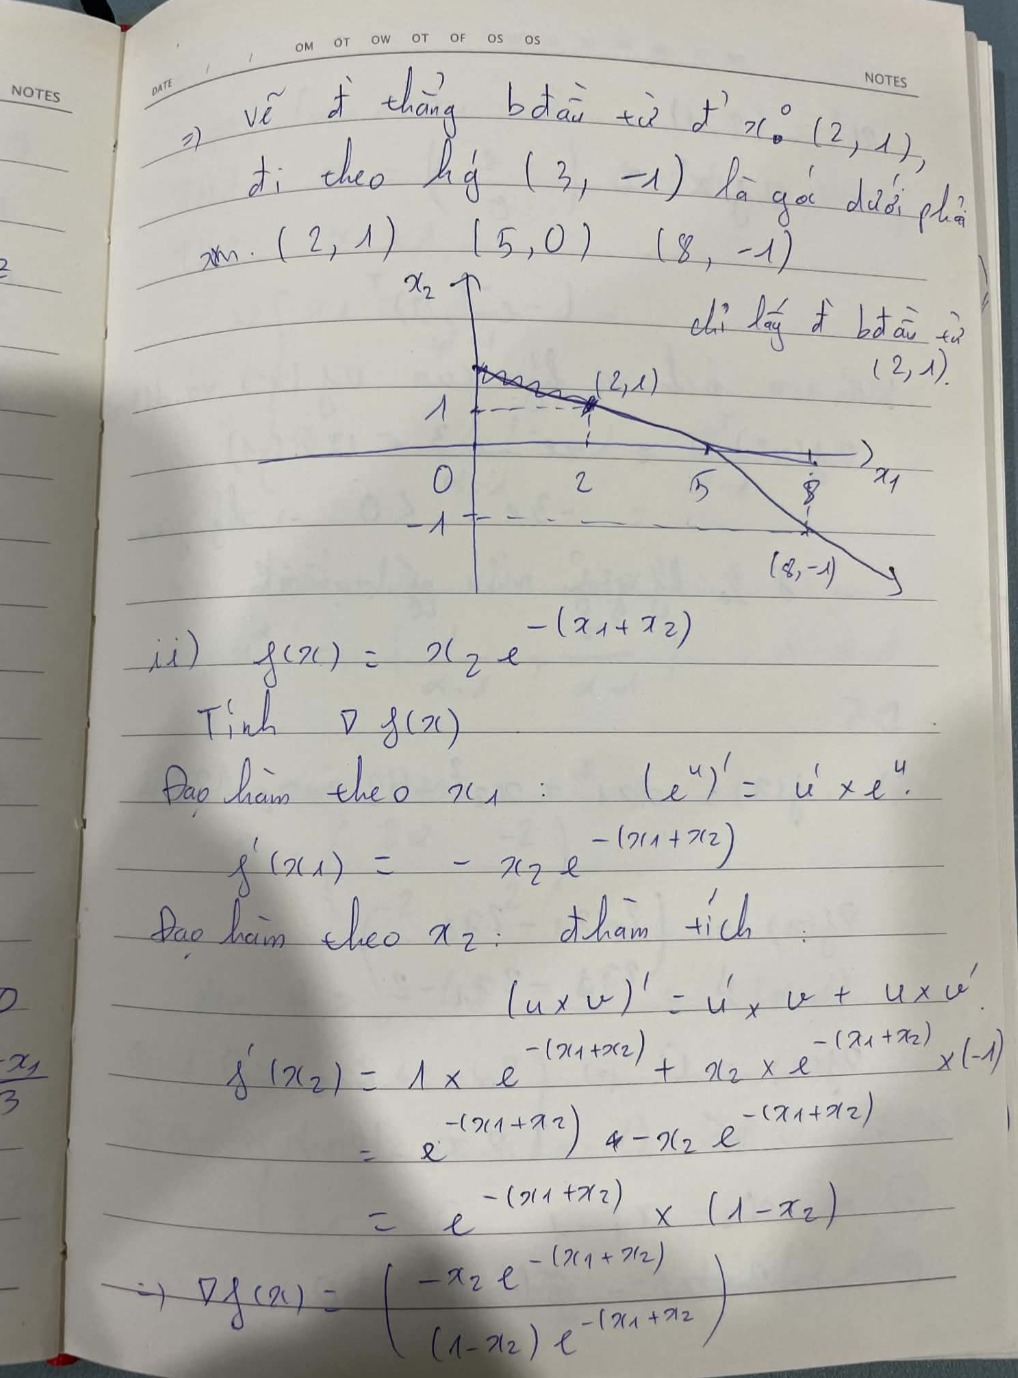
\includegraphics[width=.98\textwidth,height=.82\textheight,keepaspectratio]{bai_lam_them_1_assets/page-047.jpg}\end{center}
\clearpage
\phantomsection\label{src:048}
\noindent\textbf{Ảnh nguồn 048}\par\medskip
\begin{center}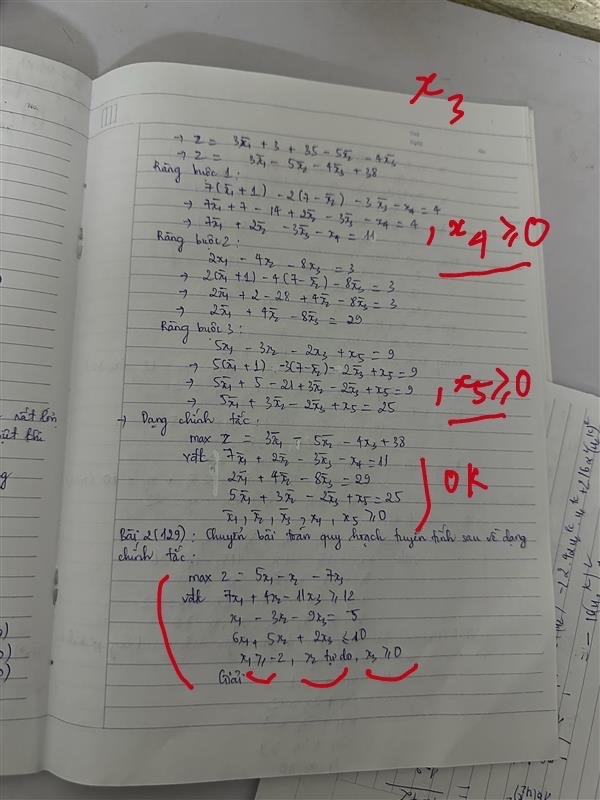
\includegraphics[width=.98\textwidth,height=.82\textheight,keepaspectratio]{bai_lam_them_1_assets/page-048.jpg}\end{center}
\clearpage
\phantomsection\label{src:049}
\noindent\textbf{Ảnh nguồn 049}\par\medskip
\begin{center}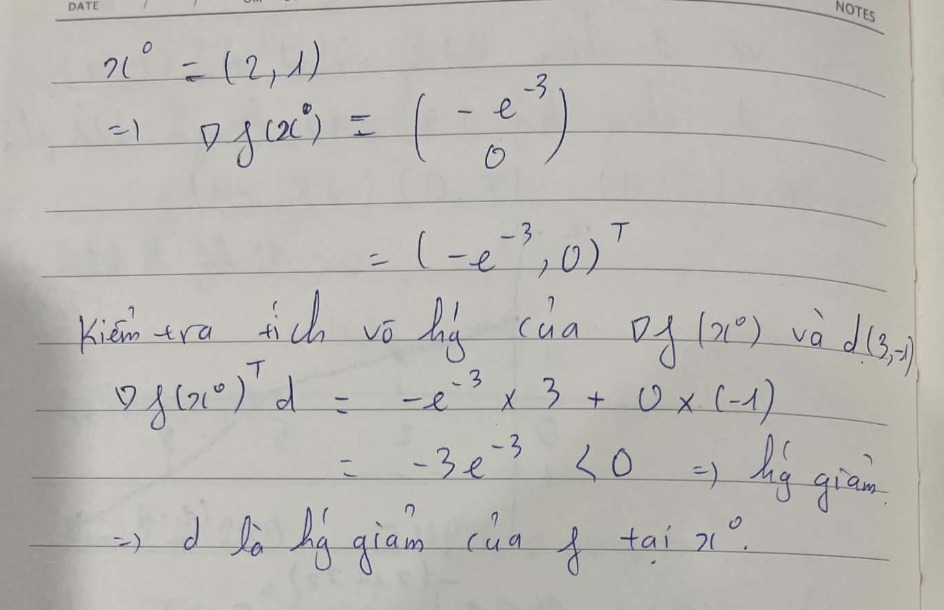
\includegraphics[width=.98\textwidth,height=.82\textheight,keepaspectratio]{bai_lam_them_1_assets/page-049.jpg}\end{center}
\clearpage
\phantomsection\label{src:050}
\noindent\textbf{Ảnh nguồn 050}\par\medskip
\begin{center}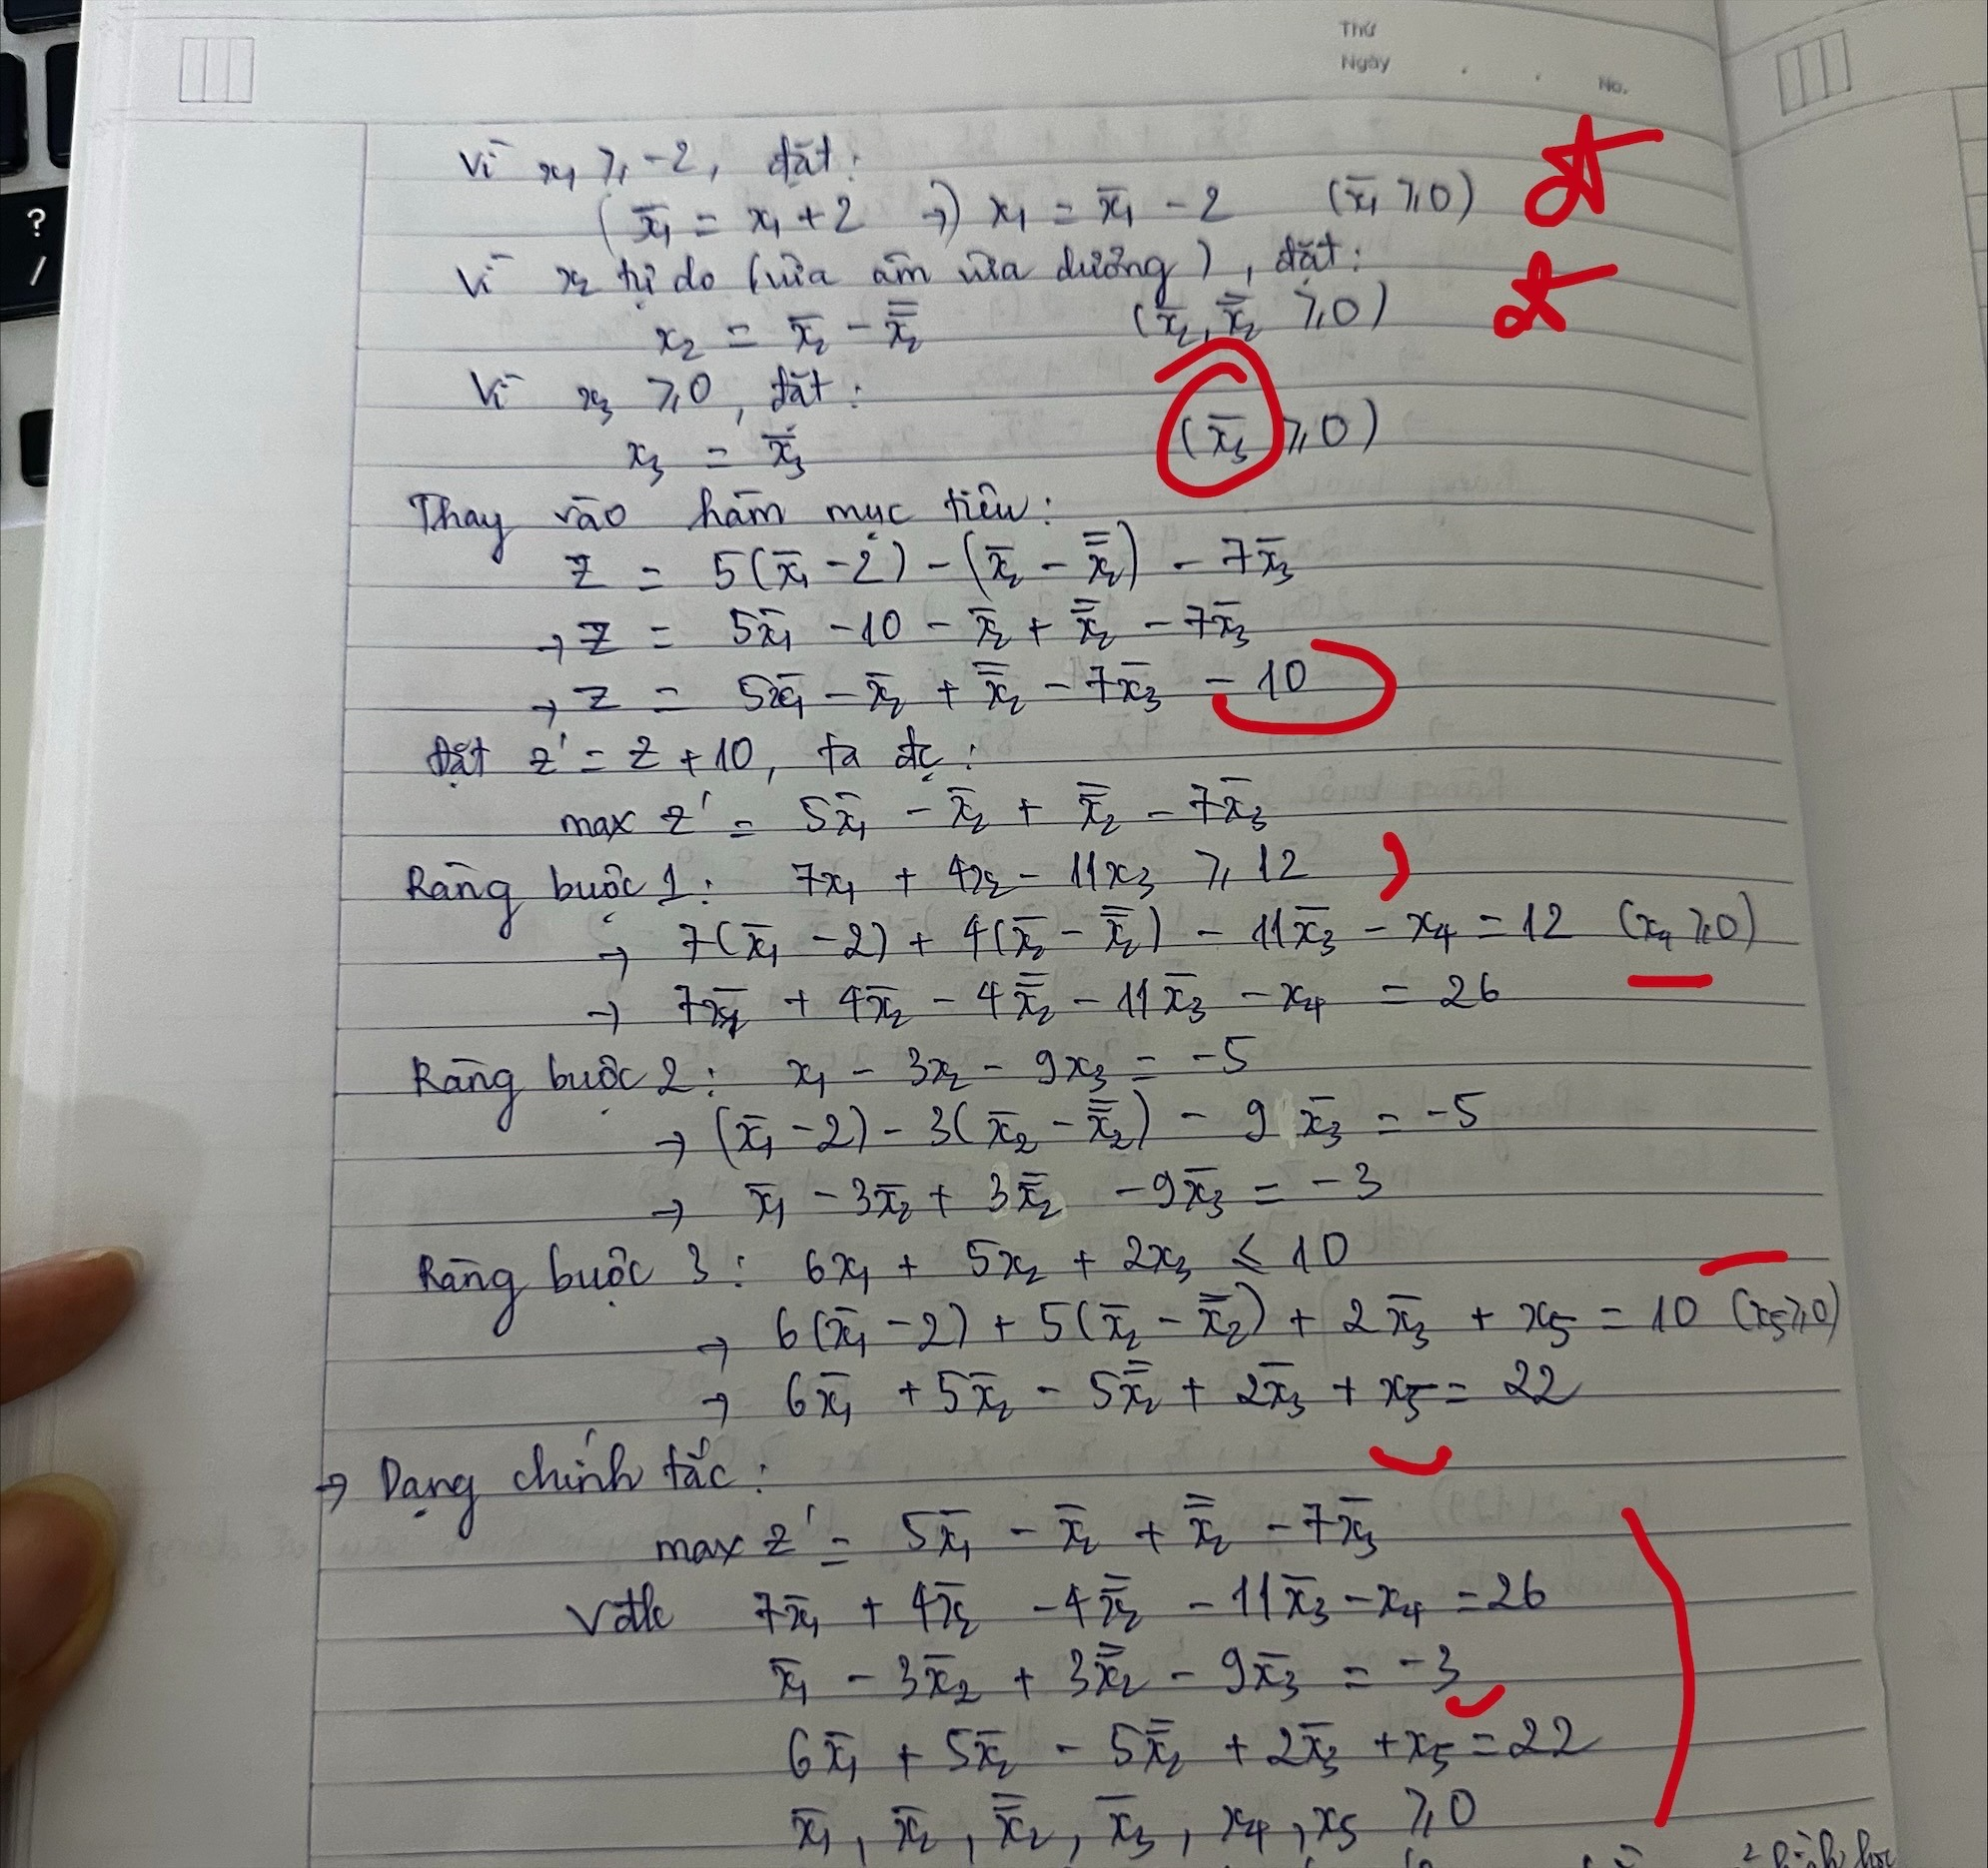
\includegraphics[width=.98\textwidth,height=.82\textheight,keepaspectratio]{bai_lam_them_1_assets/page-050.jpg}\end{center}
\clearpage
\phantomsection\label{src:051}
\noindent\textbf{Ảnh nguồn 051}\par\medskip
\begin{center}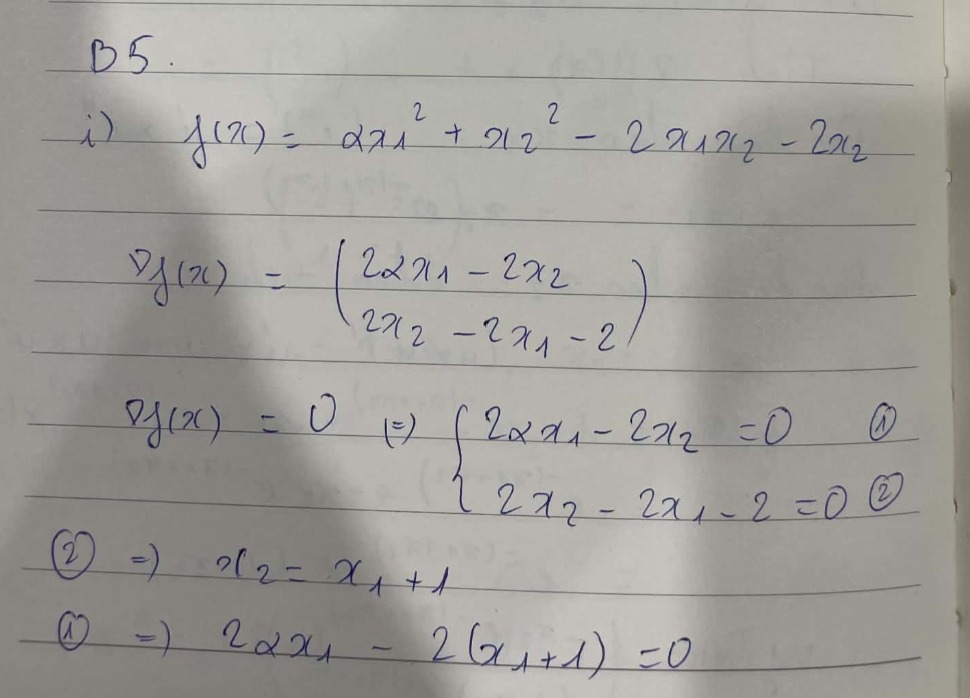
\includegraphics[width=.98\textwidth,height=.82\textheight,keepaspectratio]{bai_lam_them_1_assets/page-051.jpg}\end{center}
\clearpage
\phantomsection\label{src:052}
\noindent\textbf{Ảnh nguồn 052}\par\medskip
\begin{center}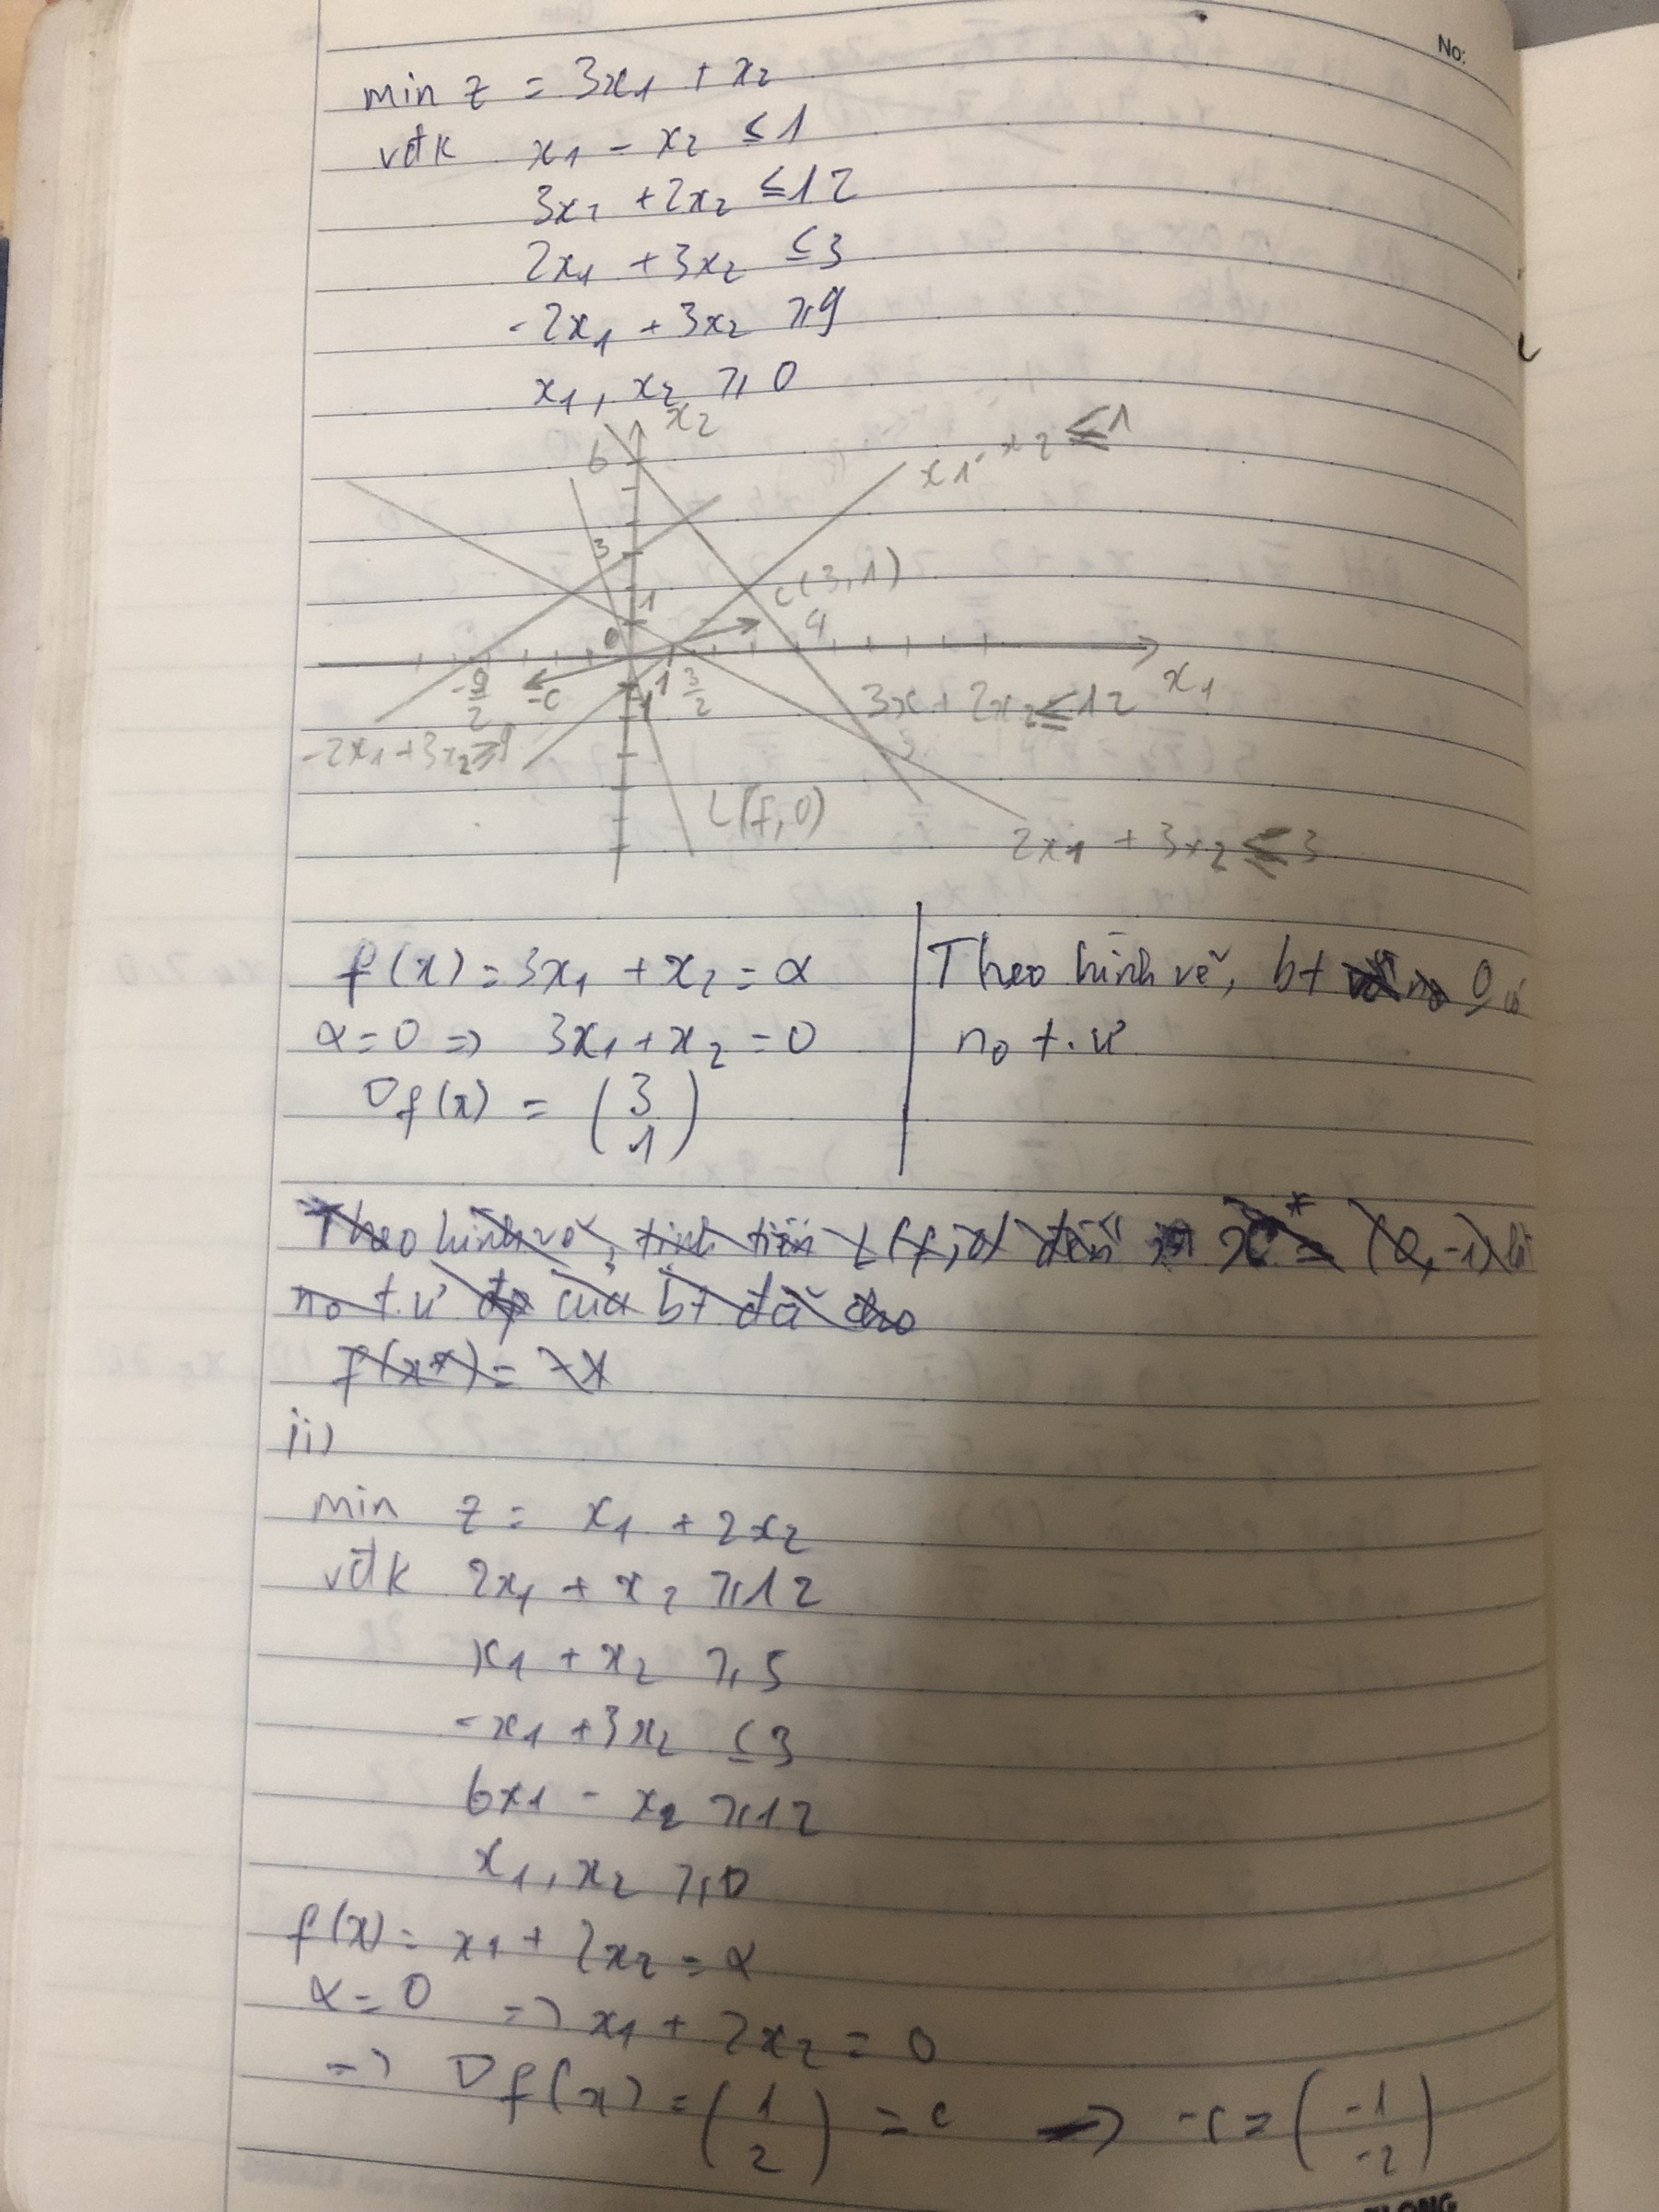
\includegraphics[width=.98\textwidth,height=.82\textheight,keepaspectratio]{bai_lam_them_1_assets/page-052.jpg}\end{center}
\clearpage
\phantomsection\label{src:053}
\noindent\textbf{Ảnh nguồn 053}\par\medskip
\begin{center}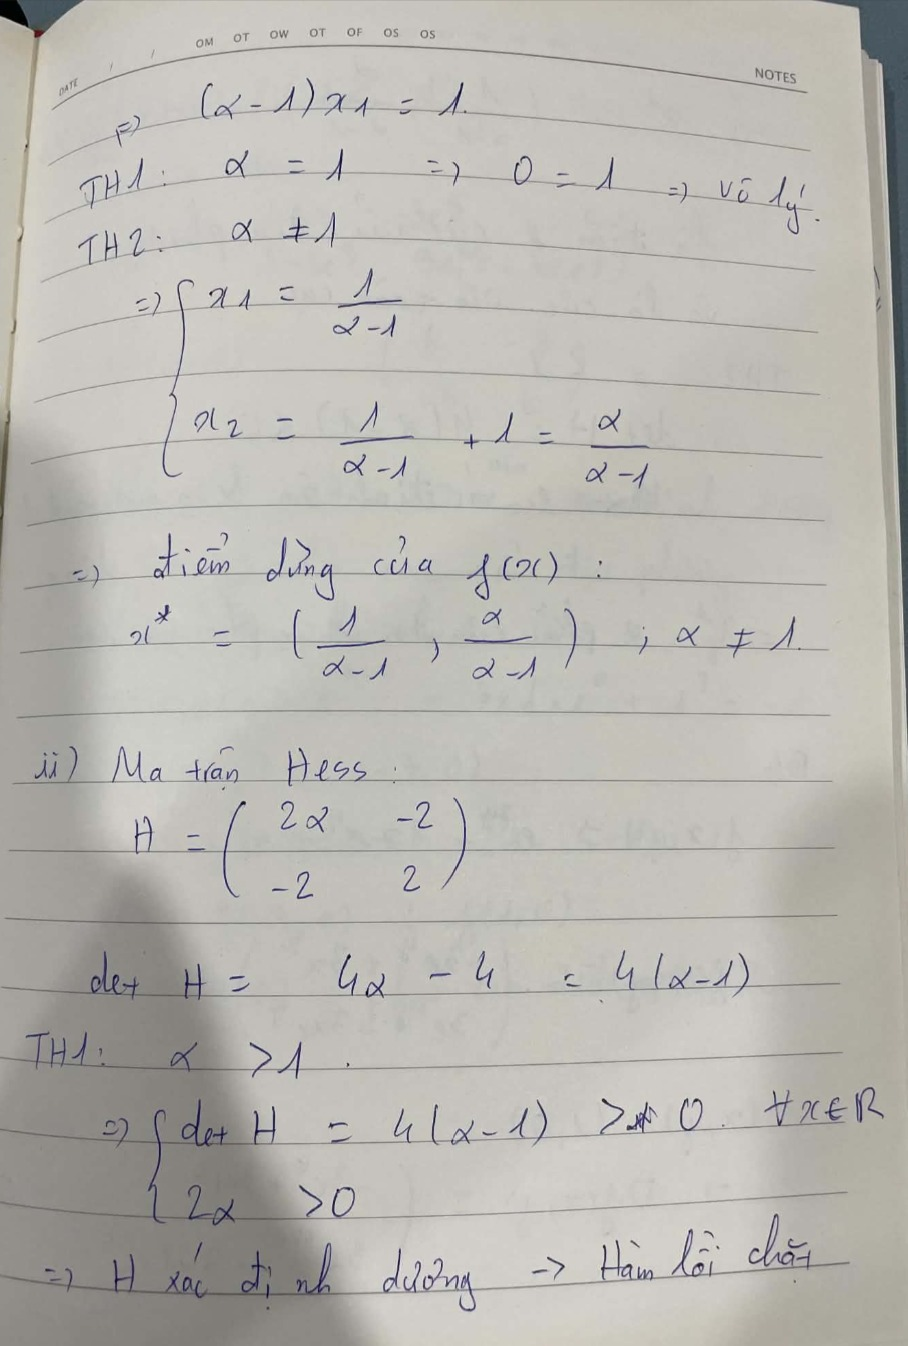
\includegraphics[width=.98\textwidth,height=.82\textheight,keepaspectratio]{bai_lam_them_1_assets/page-053.jpg}\end{center}
\clearpage
\phantomsection\label{src:054}
\noindent\textbf{Ảnh nguồn 054}\par\medskip
\begin{center}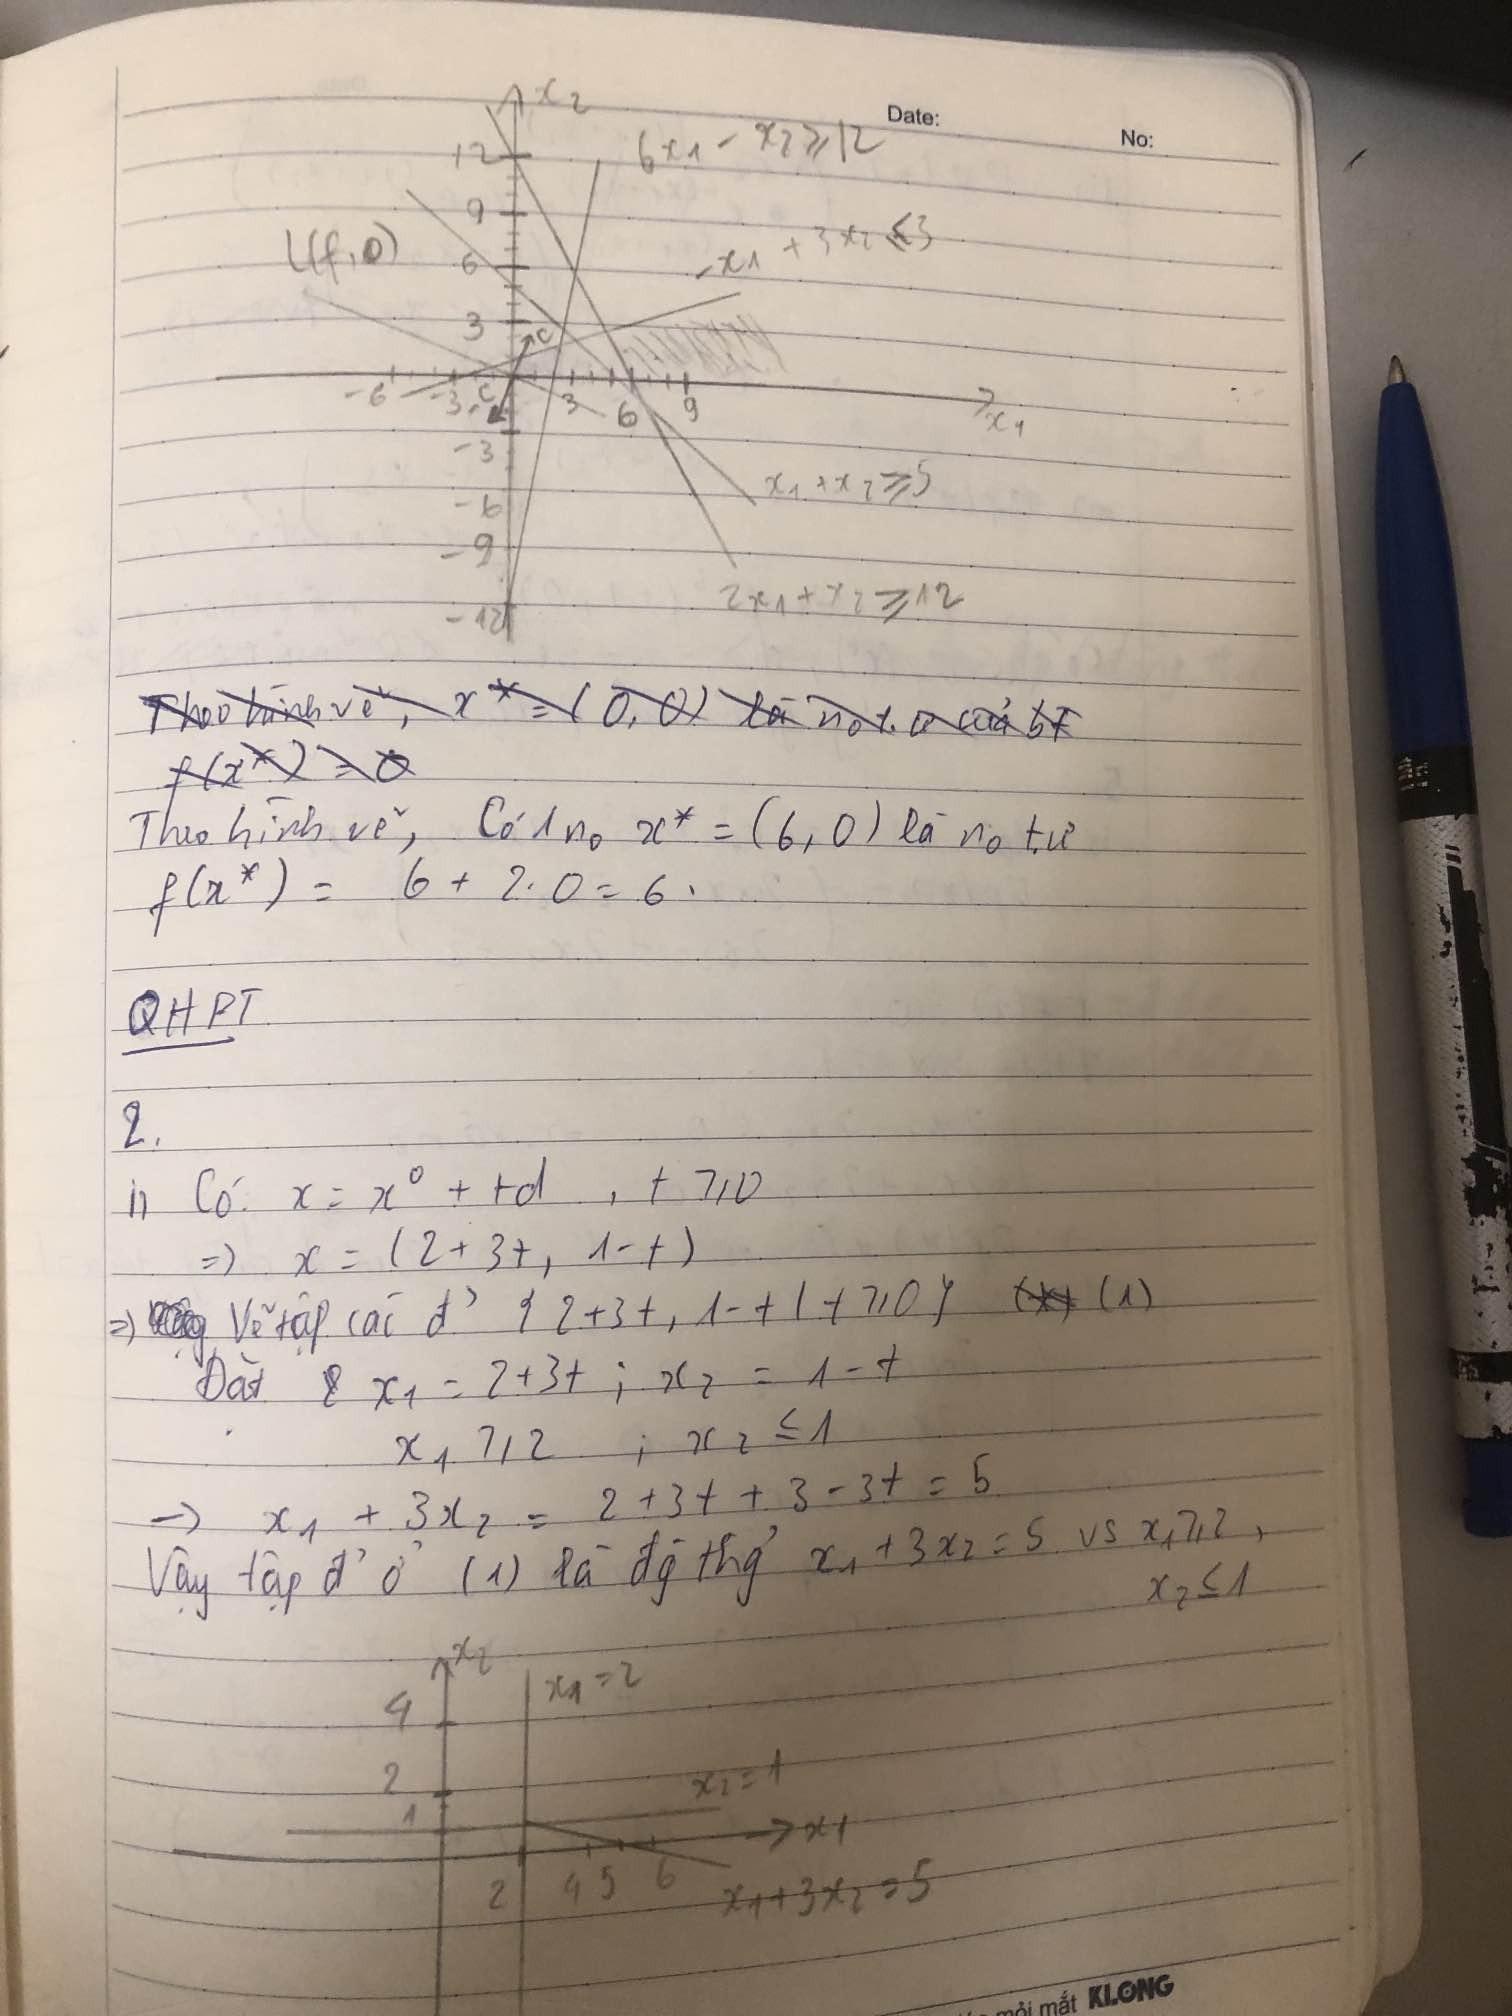
\includegraphics[width=.98\textwidth,height=.82\textheight,keepaspectratio]{bai_lam_them_1_assets/page-054.jpg}\end{center}
\clearpage
\phantomsection\label{src:055}
\noindent\textbf{Ảnh nguồn 055}\par\medskip
\begin{center}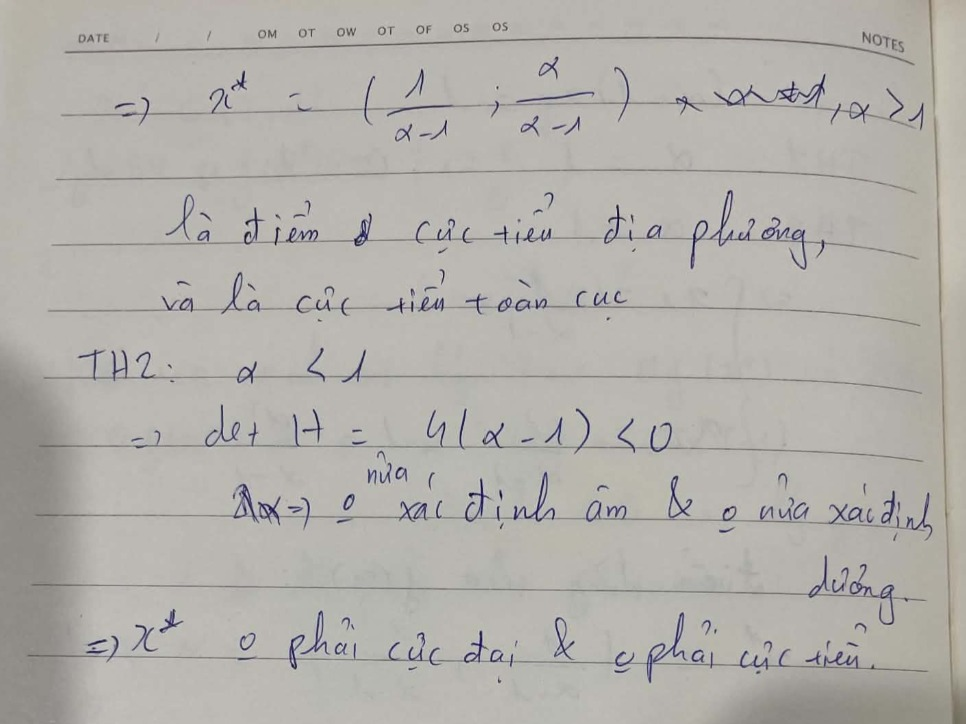
\includegraphics[width=.98\textwidth,height=.82\textheight,keepaspectratio]{bai_lam_them_1_assets/page-055.jpg}\end{center}
\clearpage
\phantomsection\label{src:056}
\noindent\textbf{Ảnh nguồn 056}\par\medskip
\begin{center}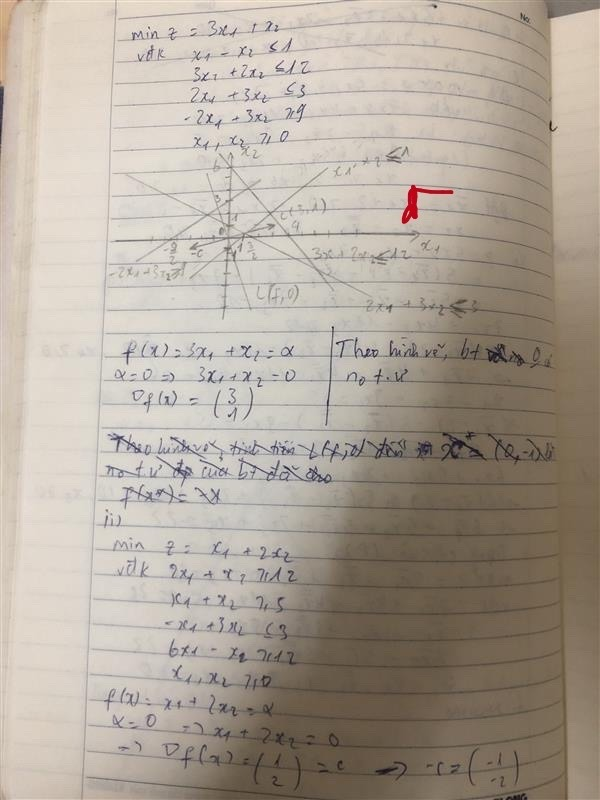
\includegraphics[width=.98\textwidth,height=.82\textheight,keepaspectratio]{bai_lam_them_1_assets/page-056.jpg}\end{center}
\clearpage
\phantomsection\label{src:057}
\noindent\textbf{Ảnh nguồn 057}\par\medskip
\begin{center}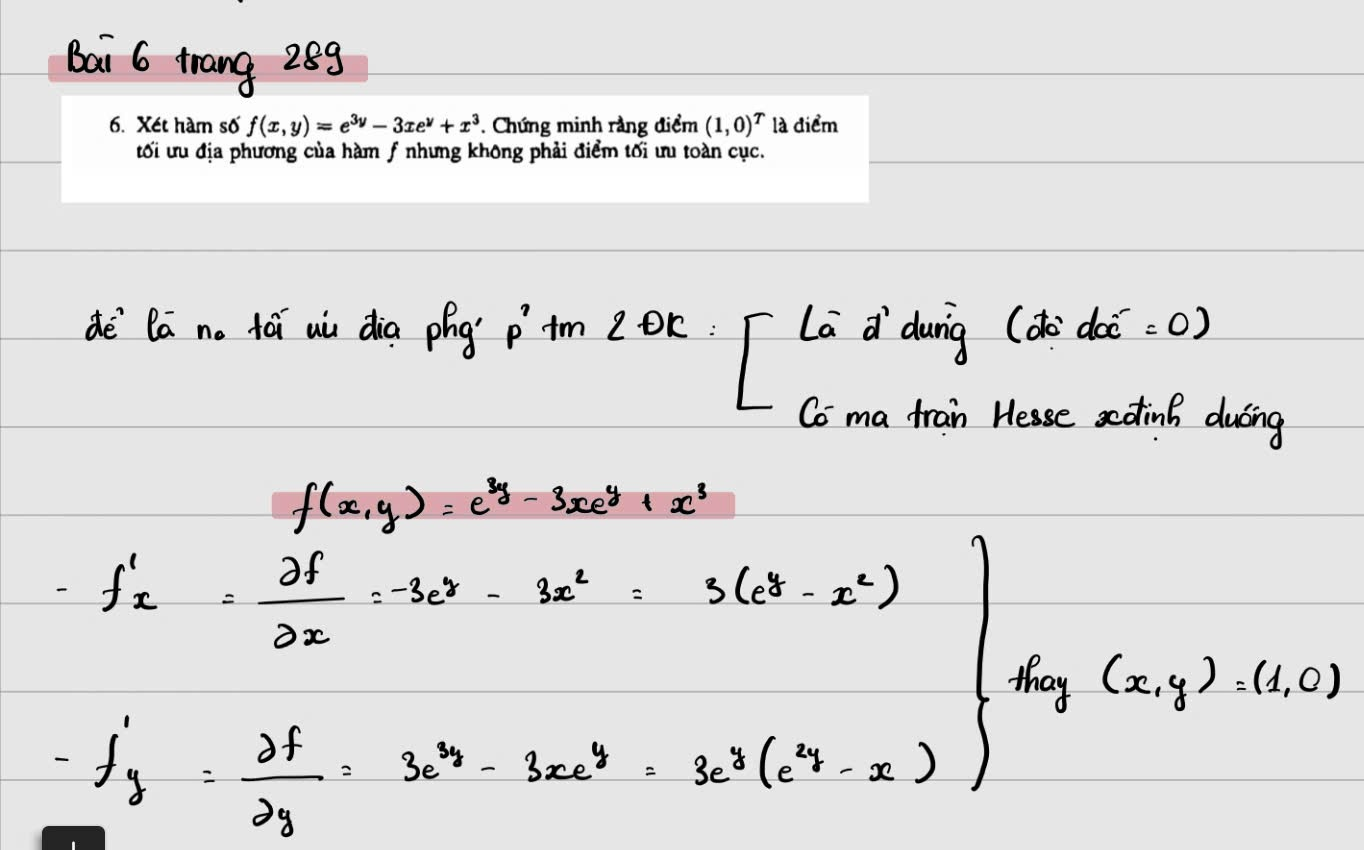
\includegraphics[width=.98\textwidth,height=.82\textheight,keepaspectratio]{bai_lam_them_1_assets/page-057.jpg}\end{center}
\clearpage
\phantomsection\label{src:058}
\noindent\textbf{Ảnh nguồn 058}\par\medskip
\begin{center}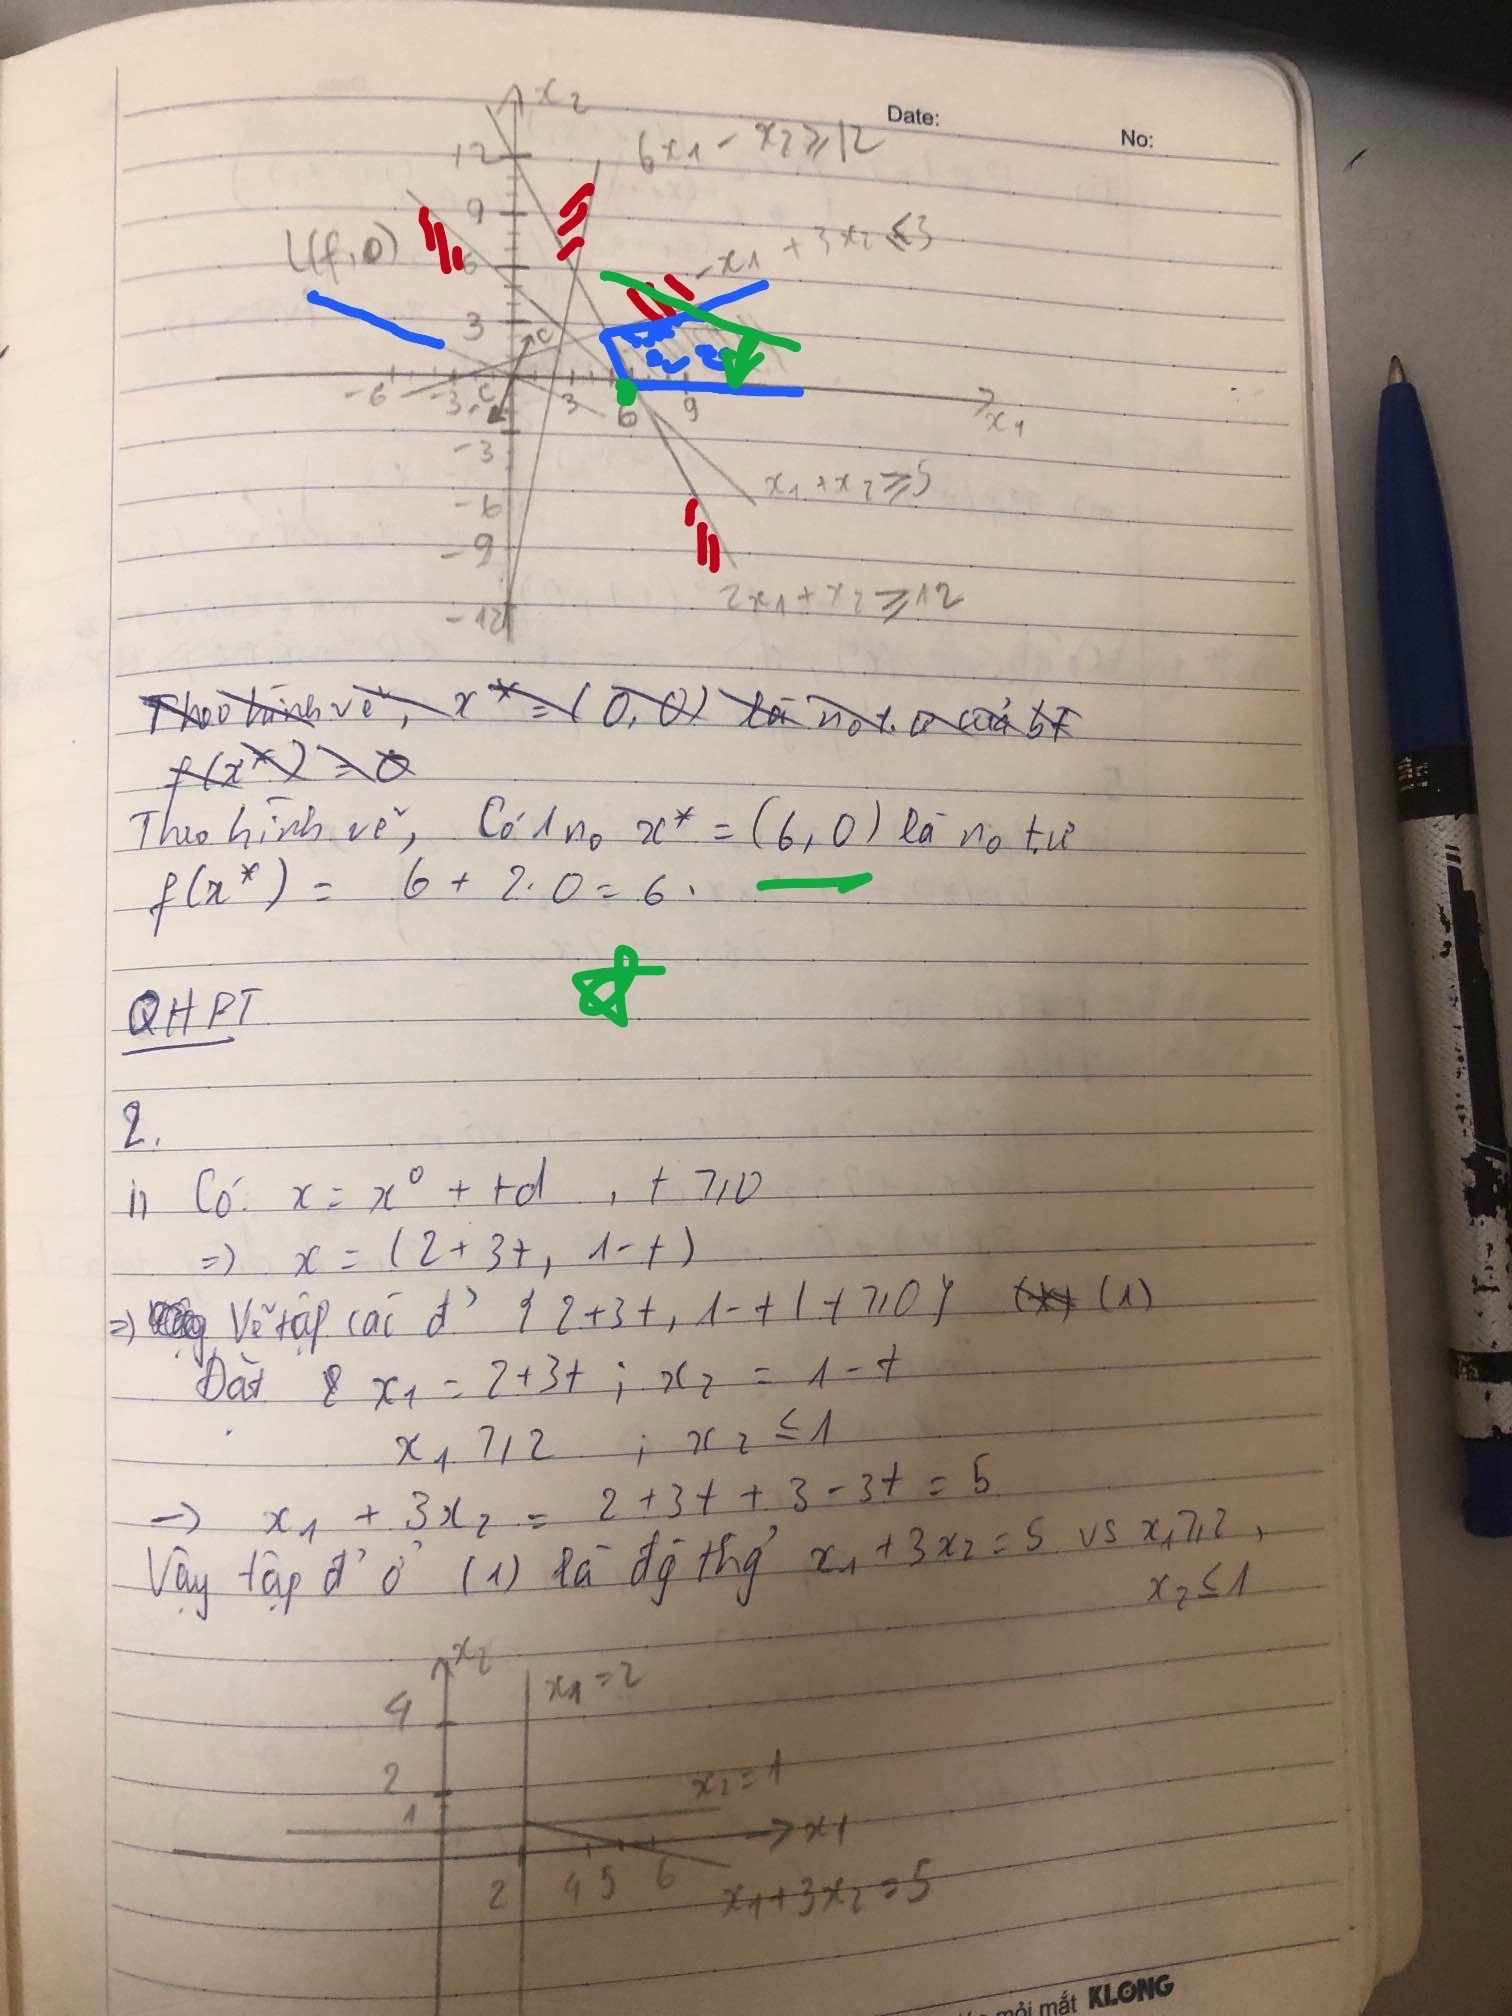
\includegraphics[width=.98\textwidth,height=.82\textheight,keepaspectratio]{bai_lam_them_1_assets/page-058.jpg}\end{center}
\clearpage
\phantomsection\label{src:059}
\noindent\textbf{Ảnh nguồn 059}\par\medskip
\begin{center}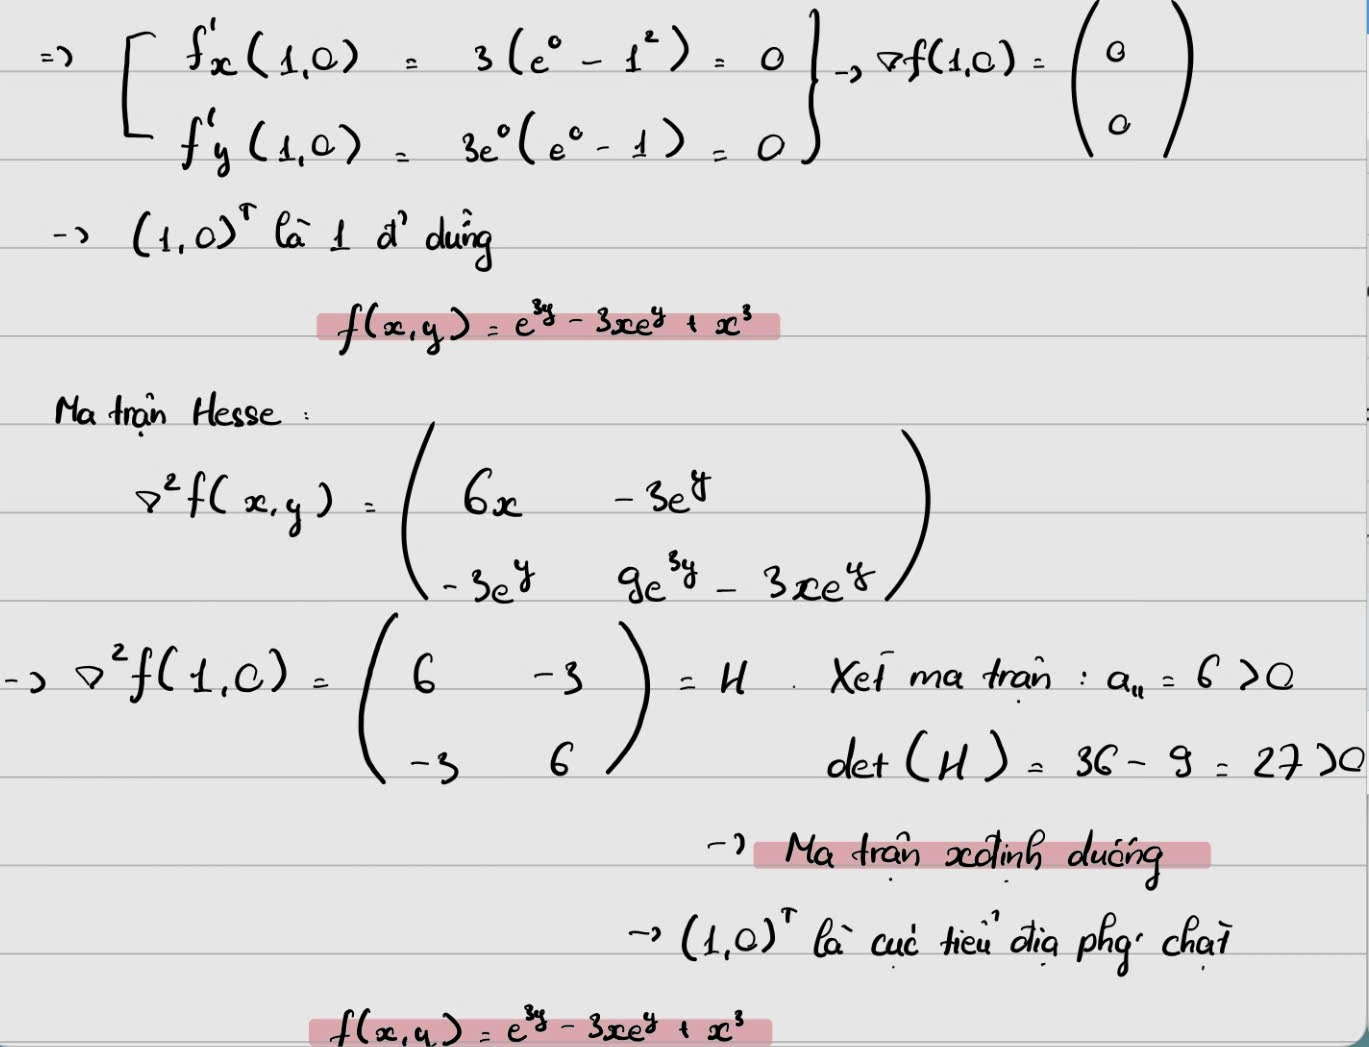
\includegraphics[width=.98\textwidth,height=.82\textheight,keepaspectratio]{bai_lam_them_1_assets/page-059.jpg}\end{center}
\clearpage
\phantomsection\label{src:060}
\noindent\textbf{Ảnh nguồn 060}\par\medskip
\begin{center}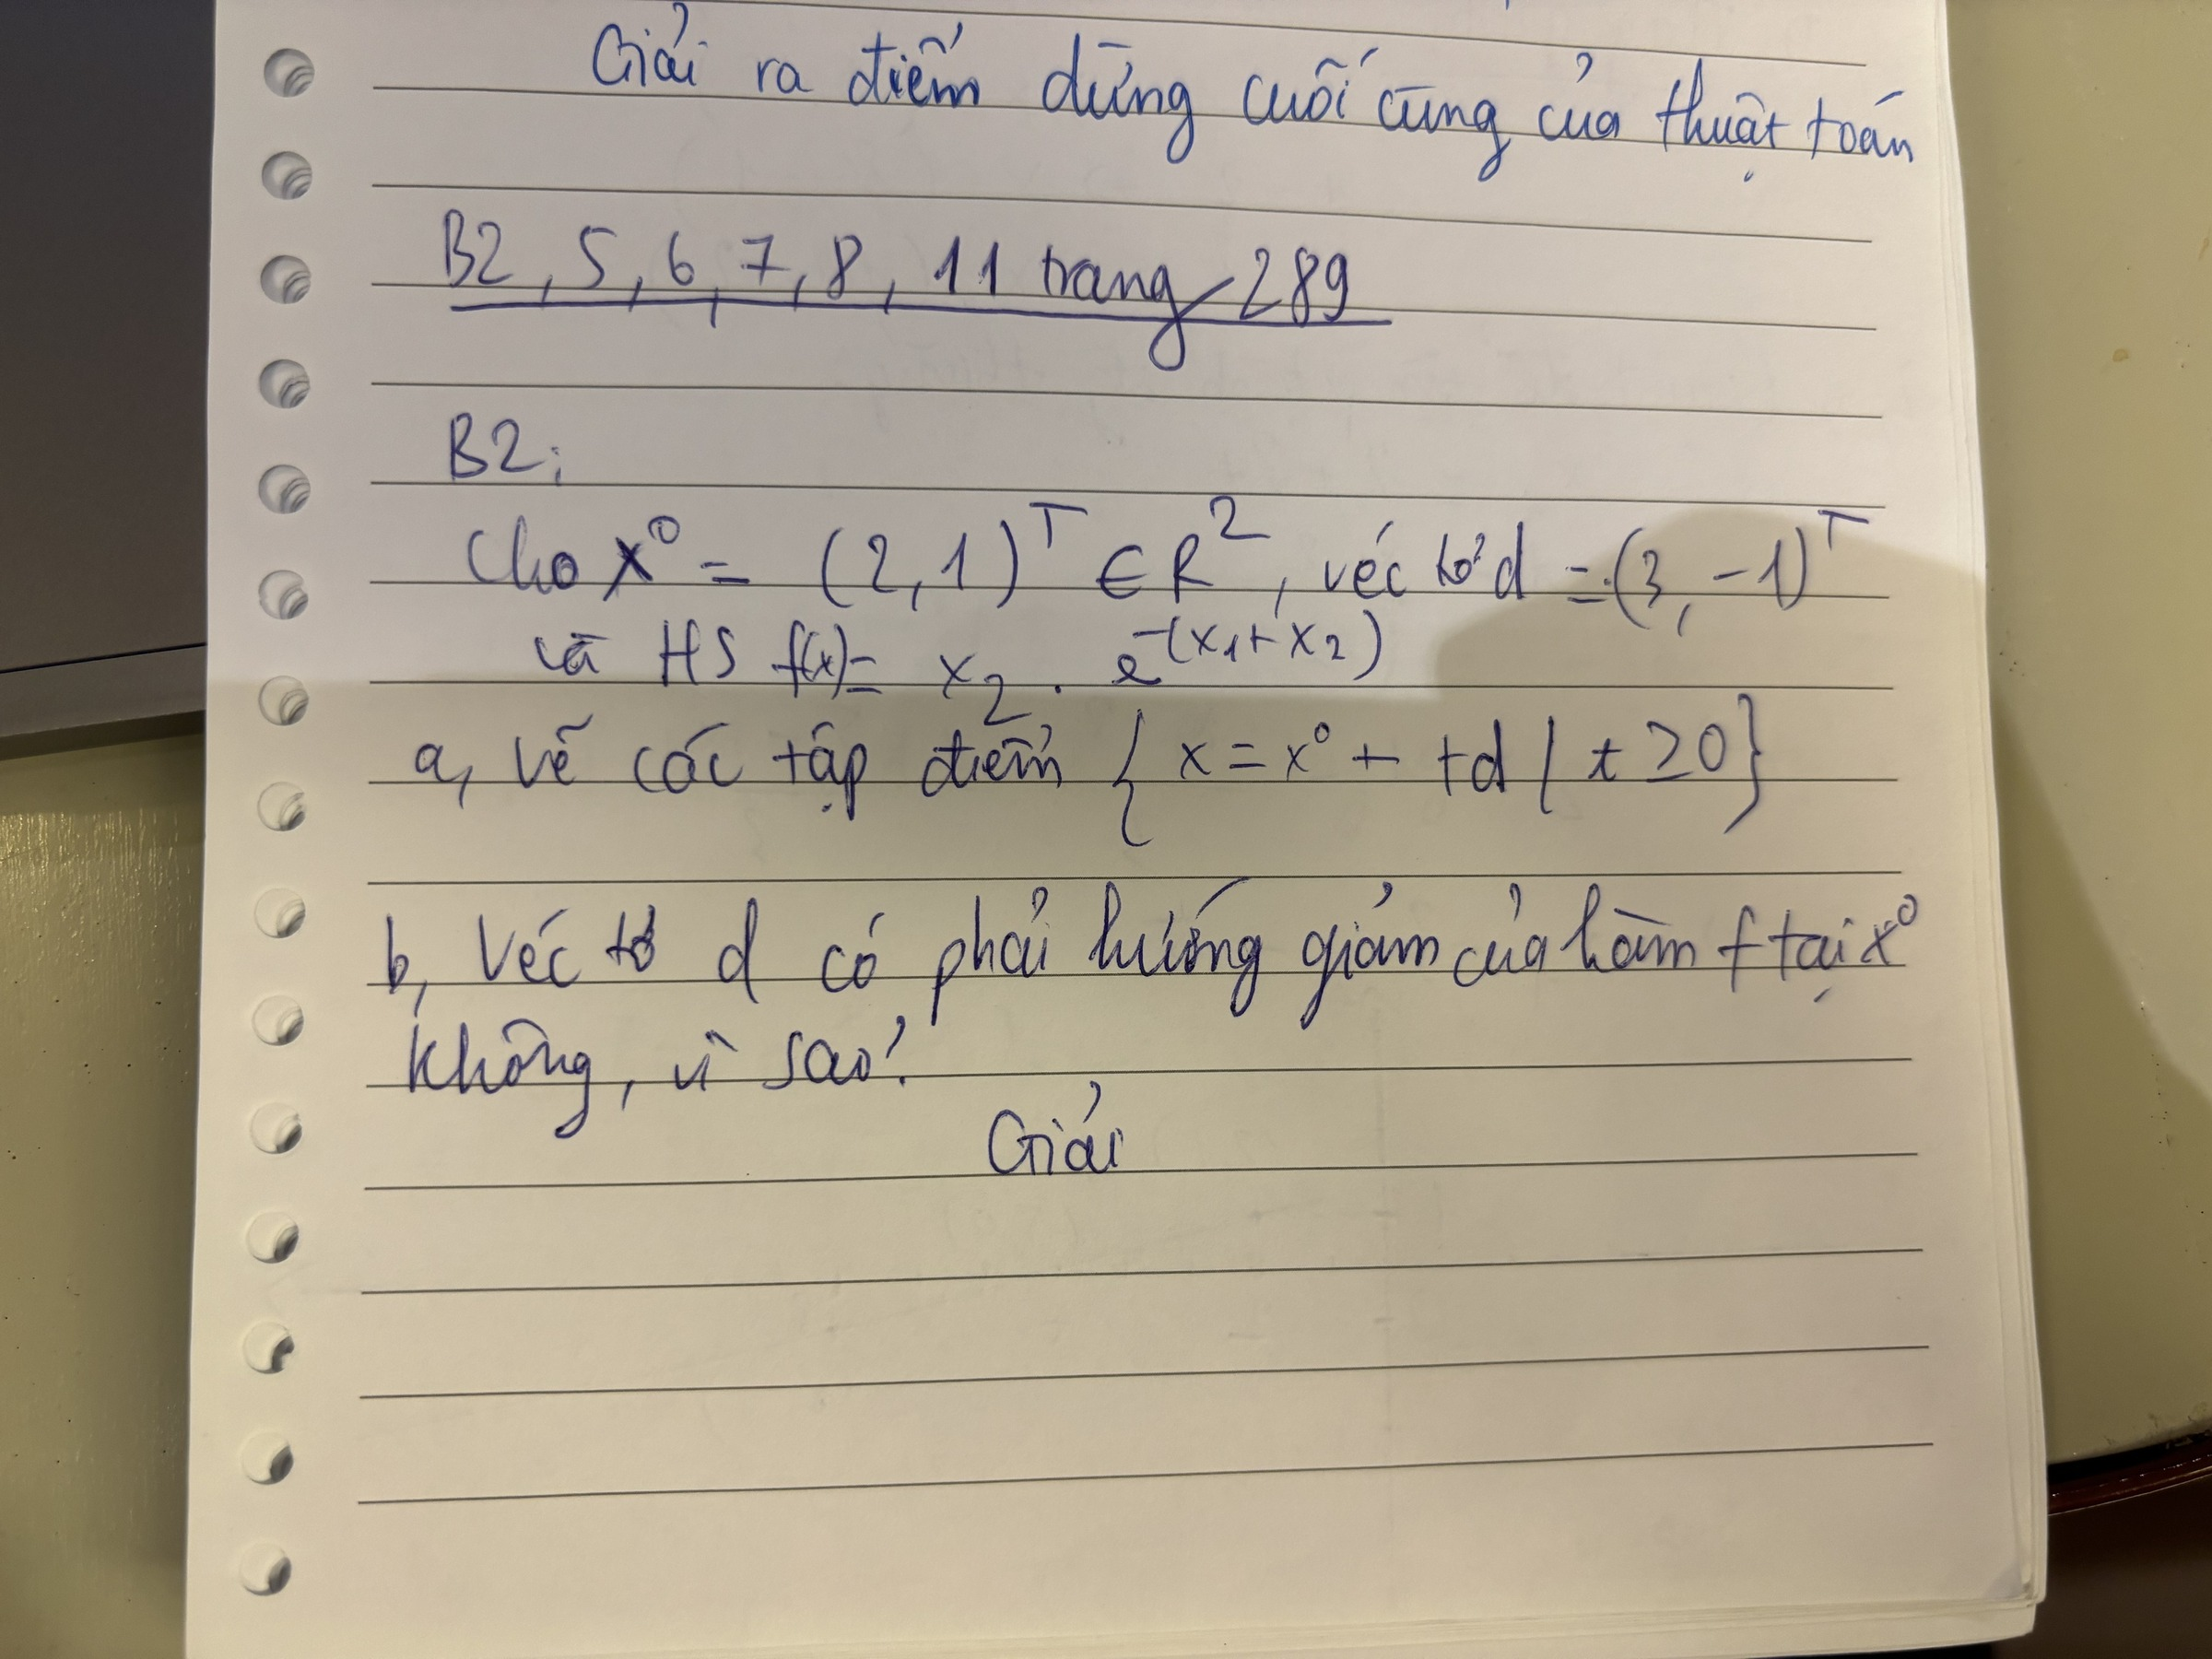
\includegraphics[width=.98\textwidth,height=.82\textheight,keepaspectratio]{bai_lam_them_1_assets/page-060.jpg}\end{center}
\clearpage
\phantomsection\label{src:061}
\noindent\textbf{Ảnh nguồn 061}\par\medskip
\begin{center}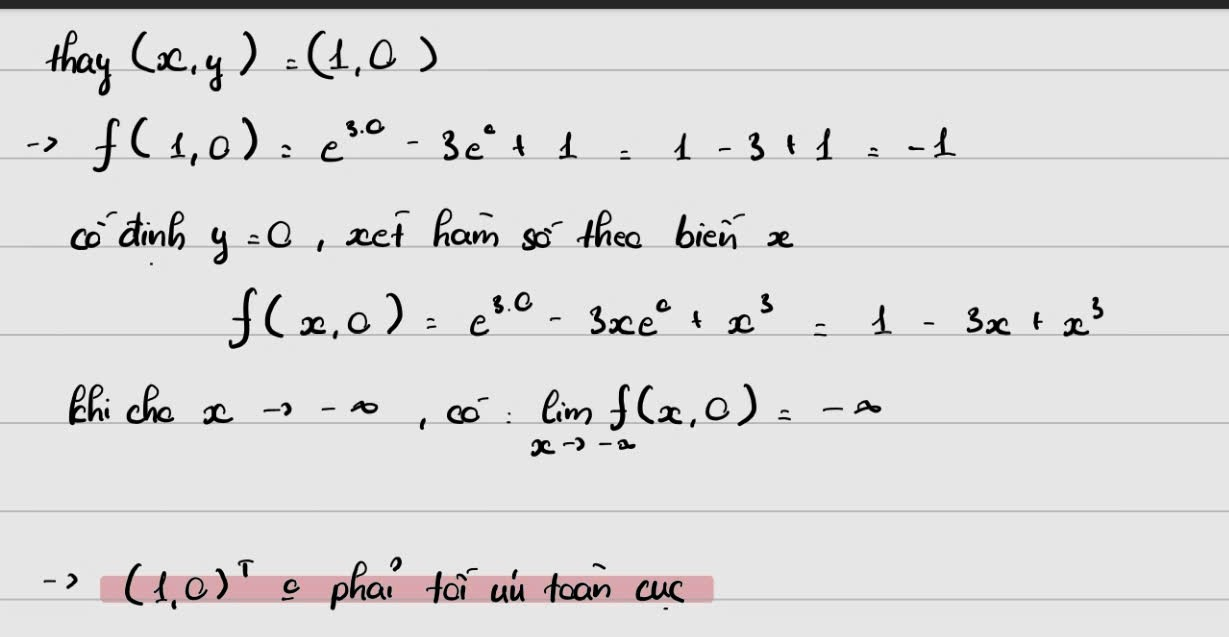
\includegraphics[width=.98\textwidth,height=.82\textheight,keepaspectratio]{bai_lam_them_1_assets/page-061.jpg}\end{center}
\clearpage
\phantomsection\label{src:062}
\noindent\textbf{Ảnh nguồn 062}\par\medskip
\begin{center}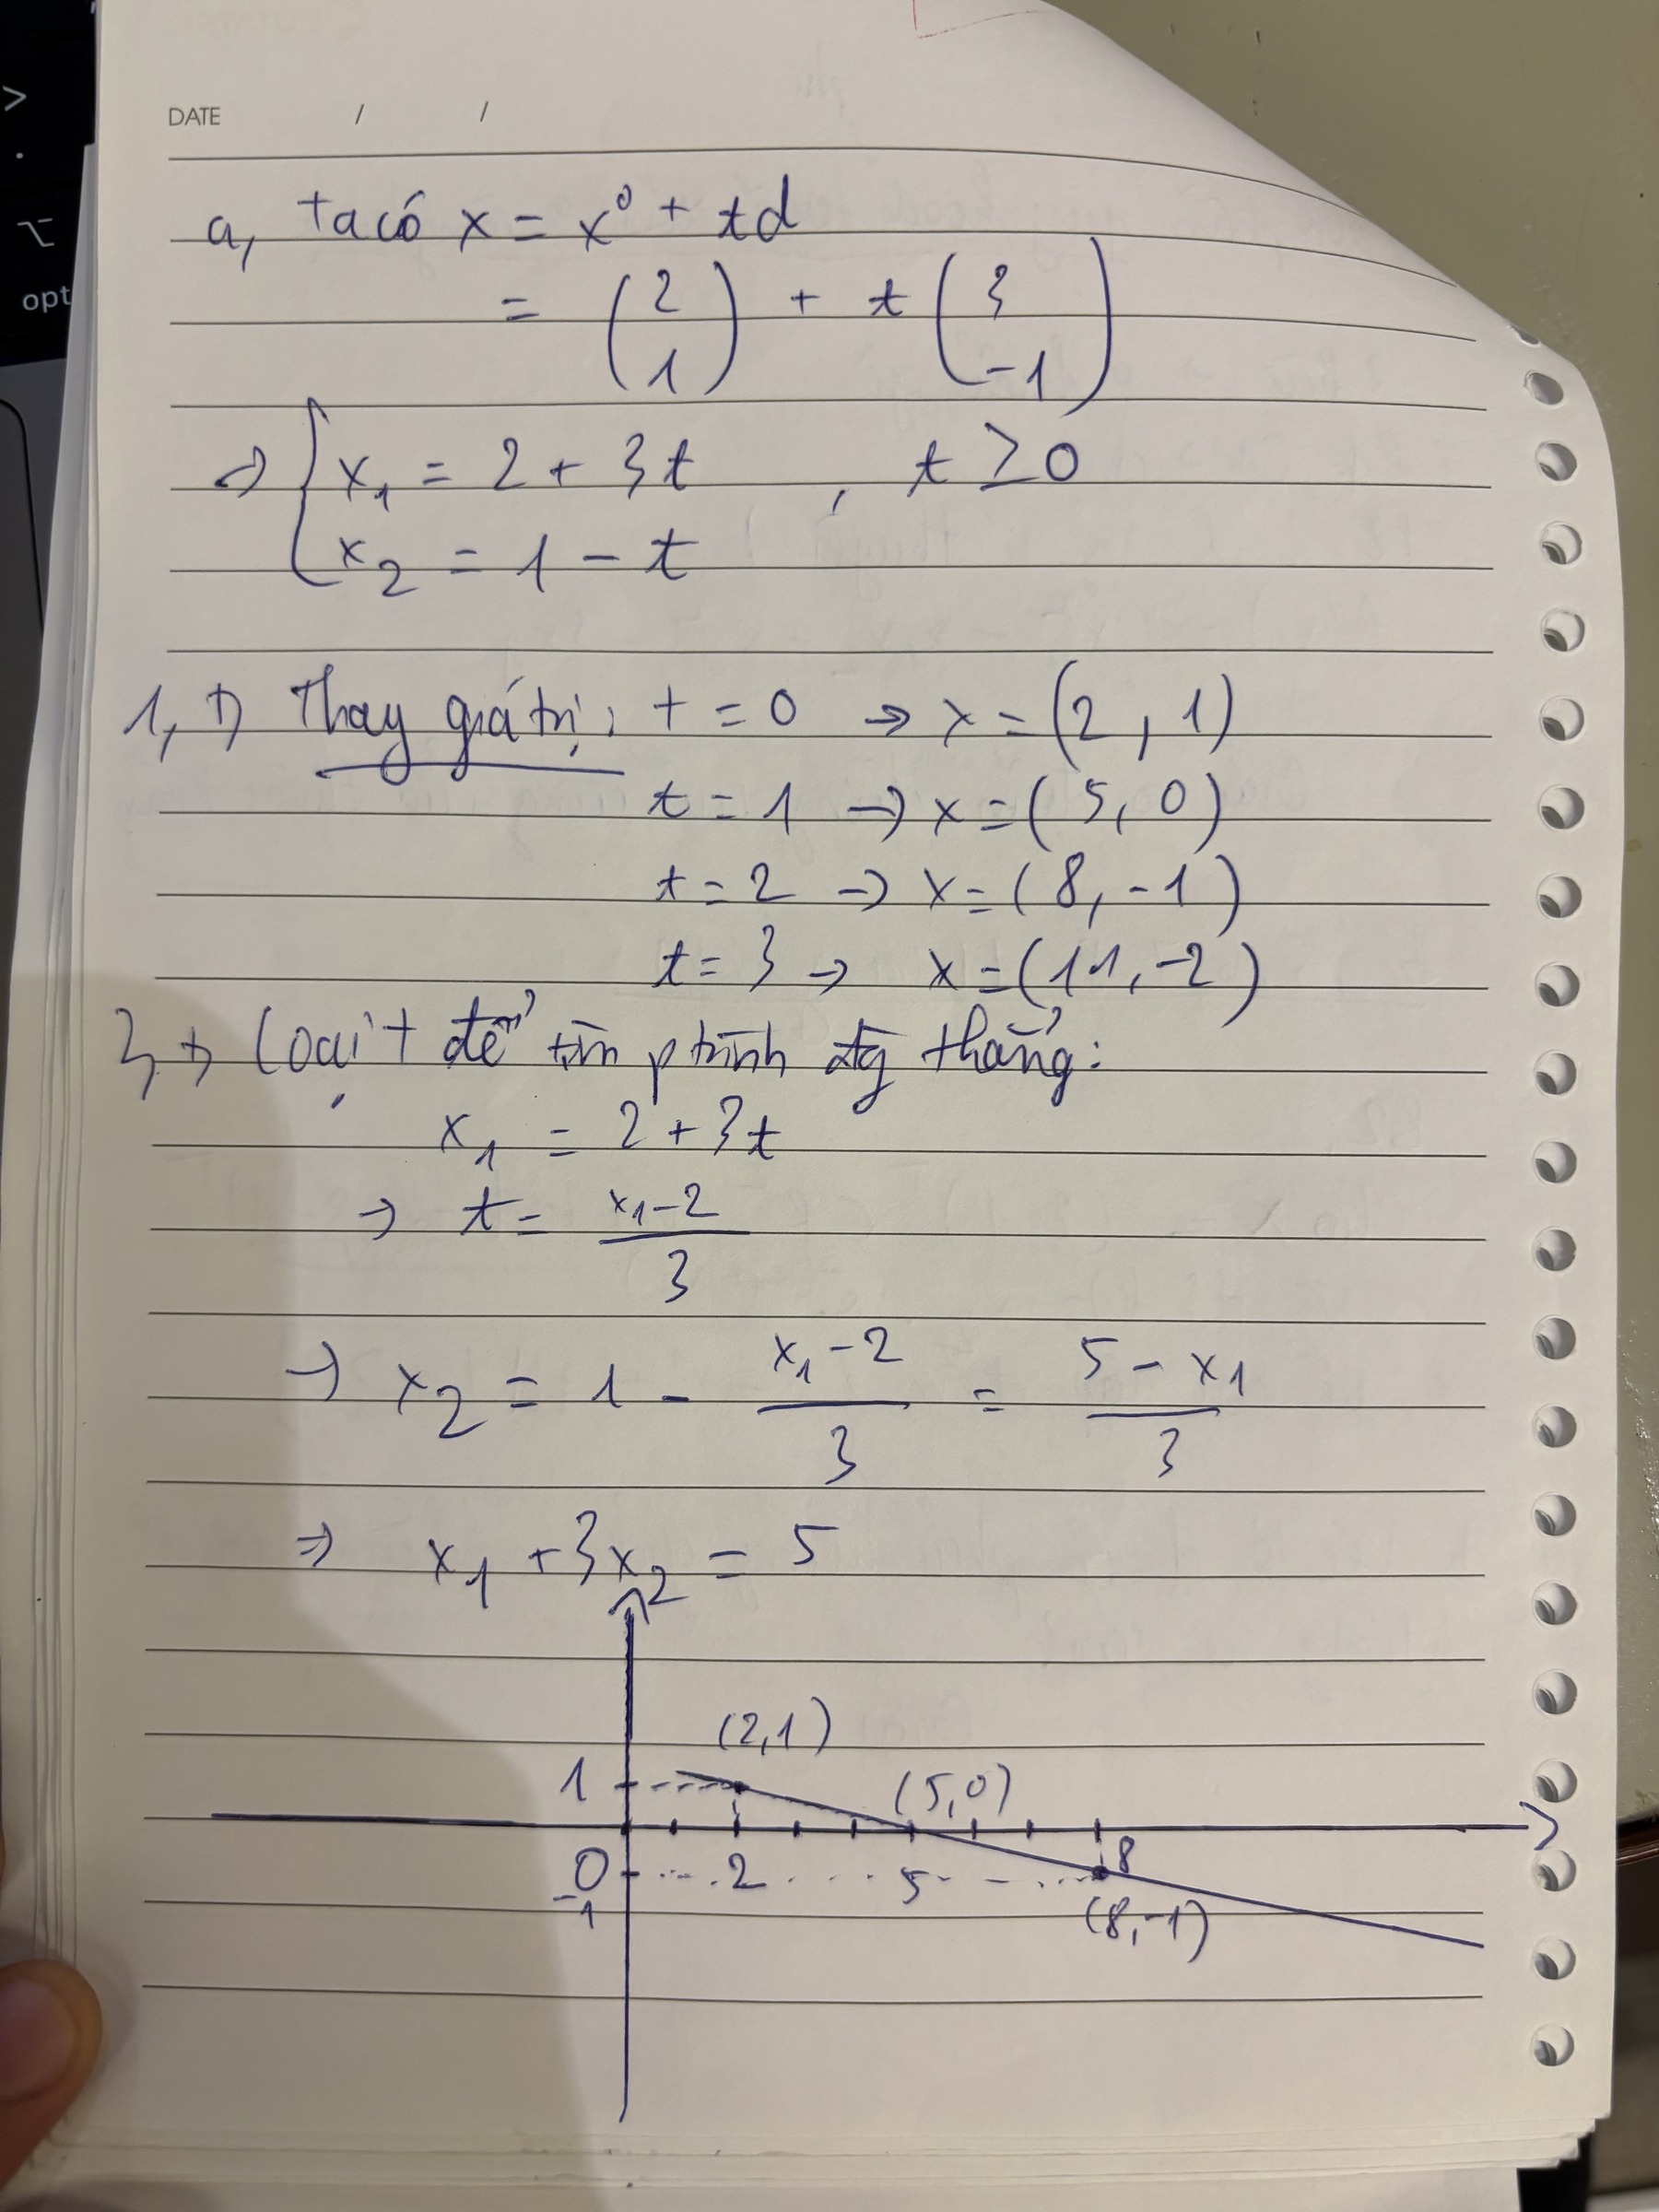
\includegraphics[width=.98\textwidth,height=.82\textheight,keepaspectratio]{bai_lam_them_1_assets/page-062.jpg}\end{center}
\clearpage
\phantomsection\label{src:063}
\noindent\textbf{Ảnh nguồn 063}\par\medskip
\begin{center}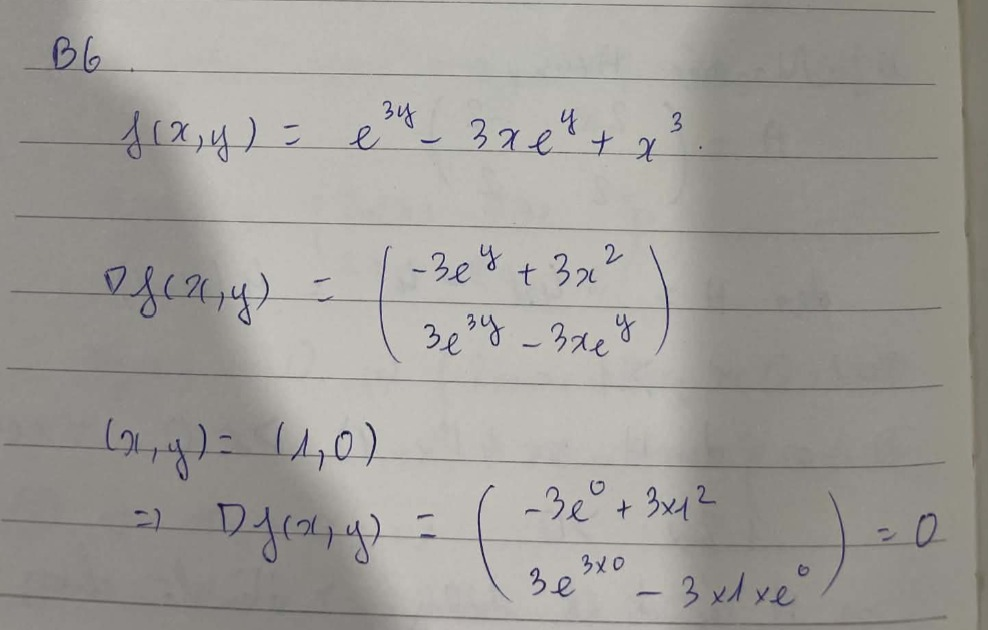
\includegraphics[width=.98\textwidth,height=.82\textheight,keepaspectratio]{bai_lam_them_1_assets/page-063.jpg}\end{center}
\clearpage
\phantomsection\label{src:064}
\noindent\textbf{Ảnh nguồn 064}\par\medskip
\begin{center}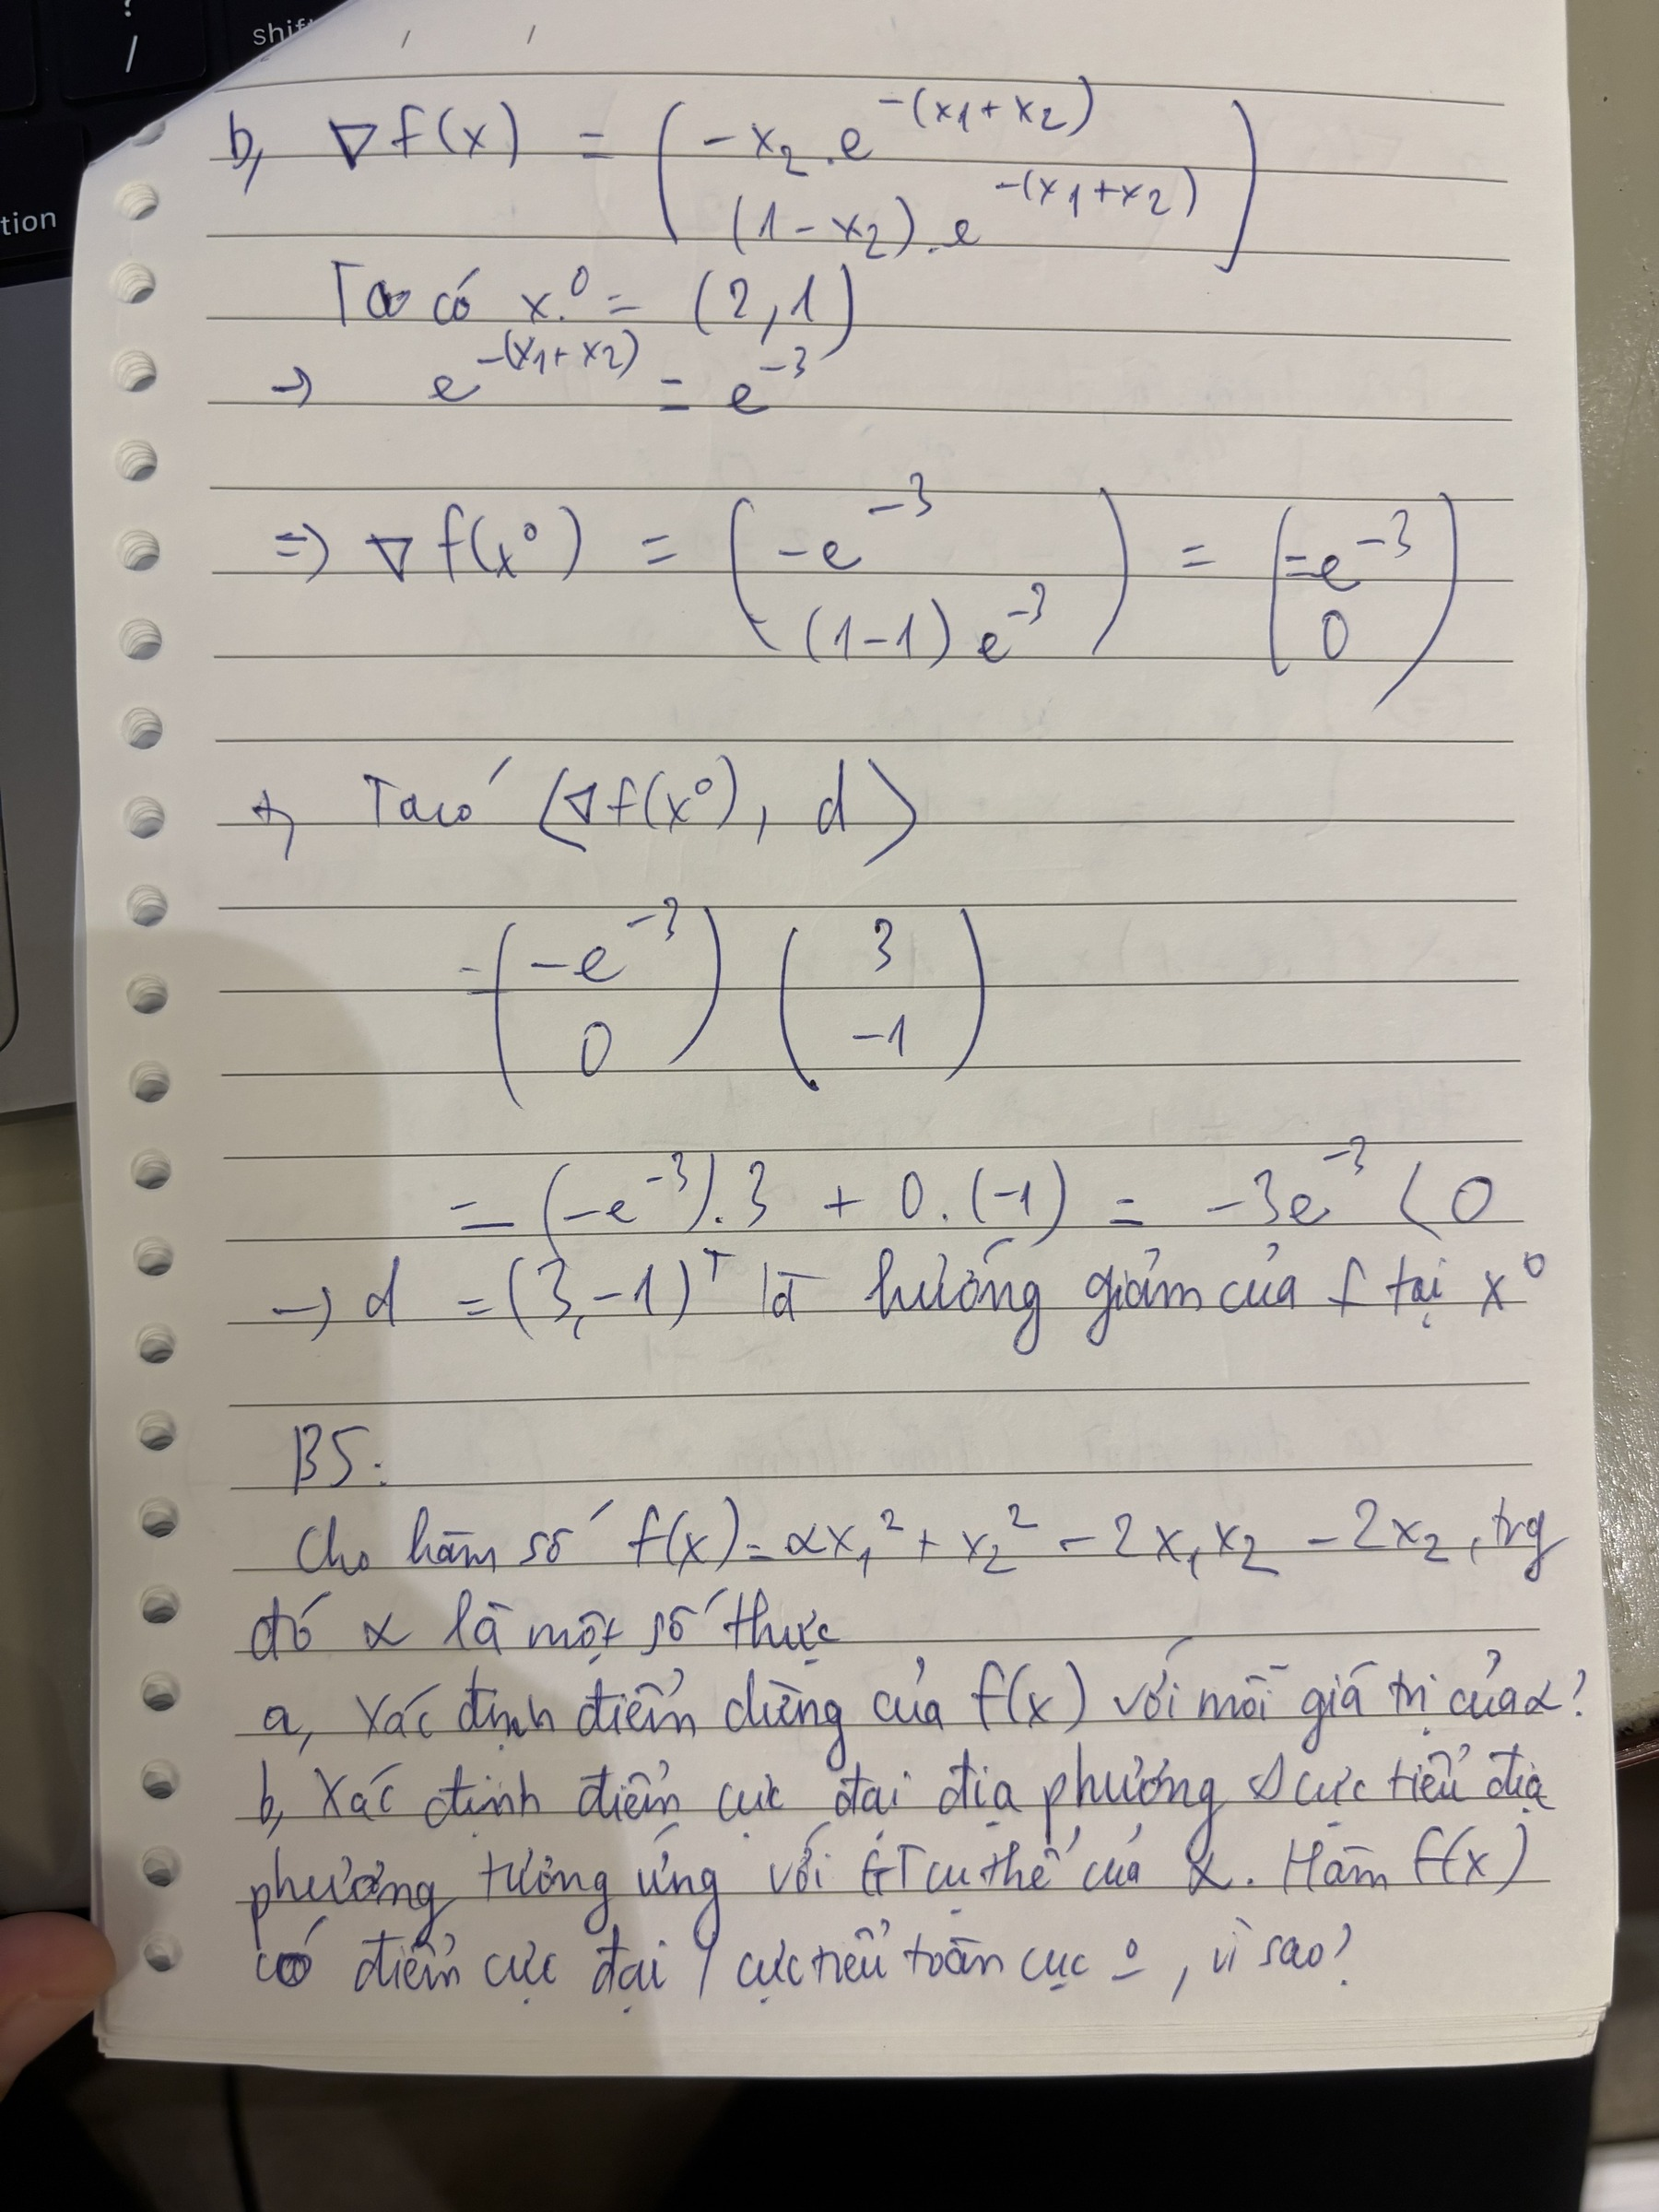
\includegraphics[width=.98\textwidth,height=.82\textheight,keepaspectratio]{bai_lam_them_1_assets/page-064.jpg}\end{center}
\clearpage
\phantomsection\label{src:065}
\noindent\textbf{Ảnh nguồn 065}\par\medskip
\begin{center}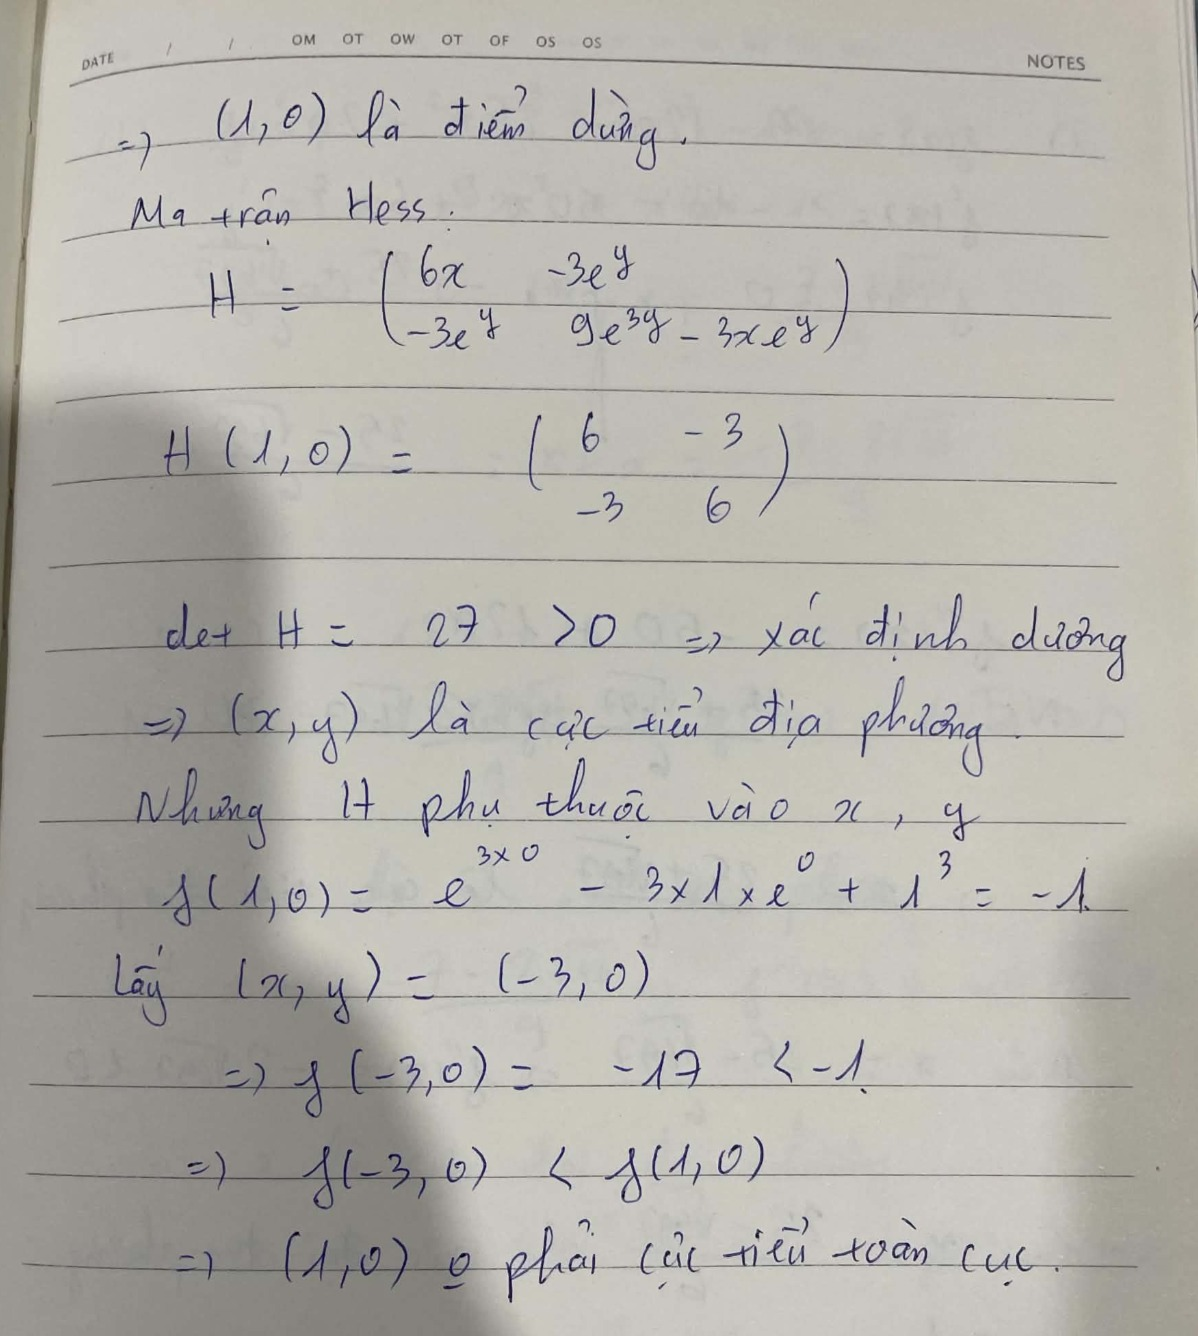
\includegraphics[width=.98\textwidth,height=.82\textheight,keepaspectratio]{bai_lam_them_1_assets/page-065.jpg}\end{center}
\clearpage
\phantomsection\label{src:066}
\noindent\textbf{Ảnh nguồn 066}\par\medskip
\begin{center}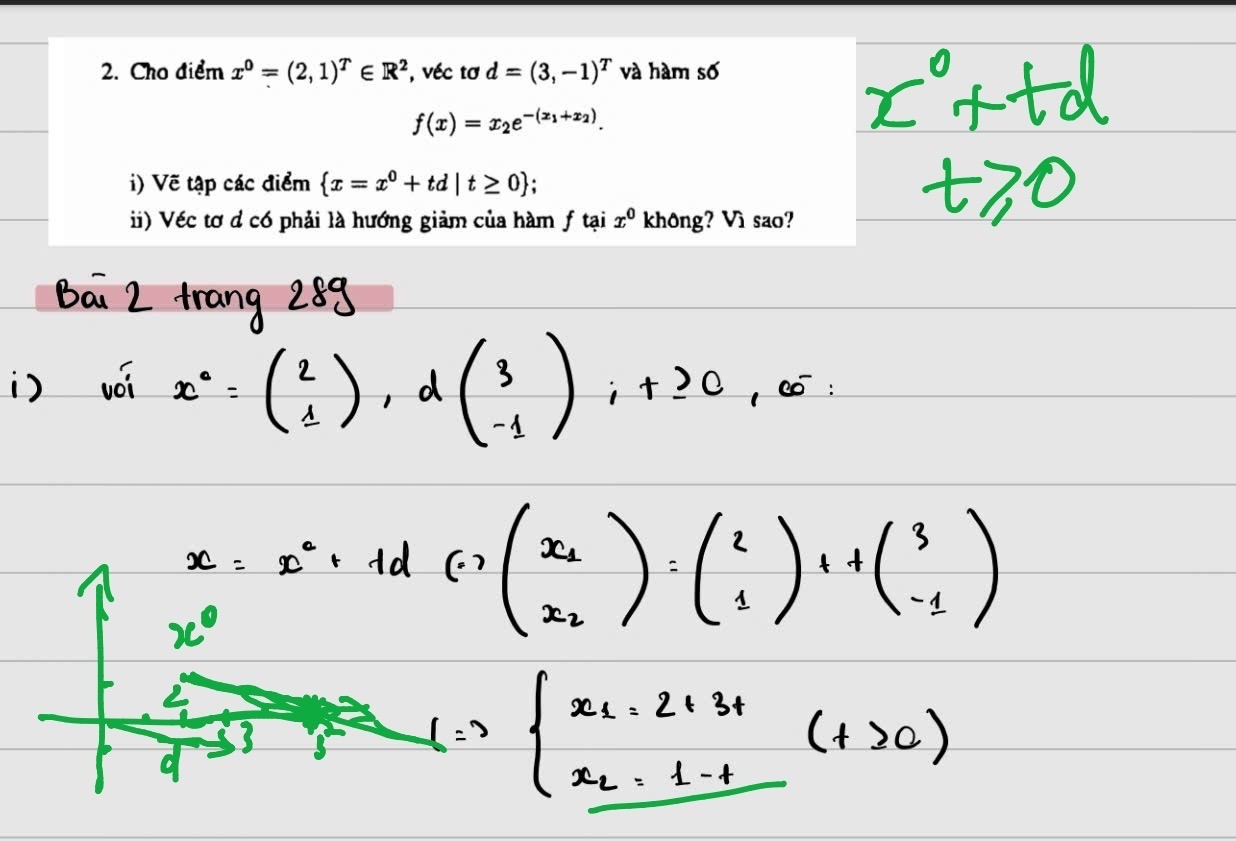
\includegraphics[width=.98\textwidth,height=.82\textheight,keepaspectratio]{bai_lam_them_1_assets/page-066.jpg}\end{center}
\clearpage
\phantomsection\label{src:067}
\noindent\textbf{Ảnh nguồn 067}\par\medskip
\begin{center}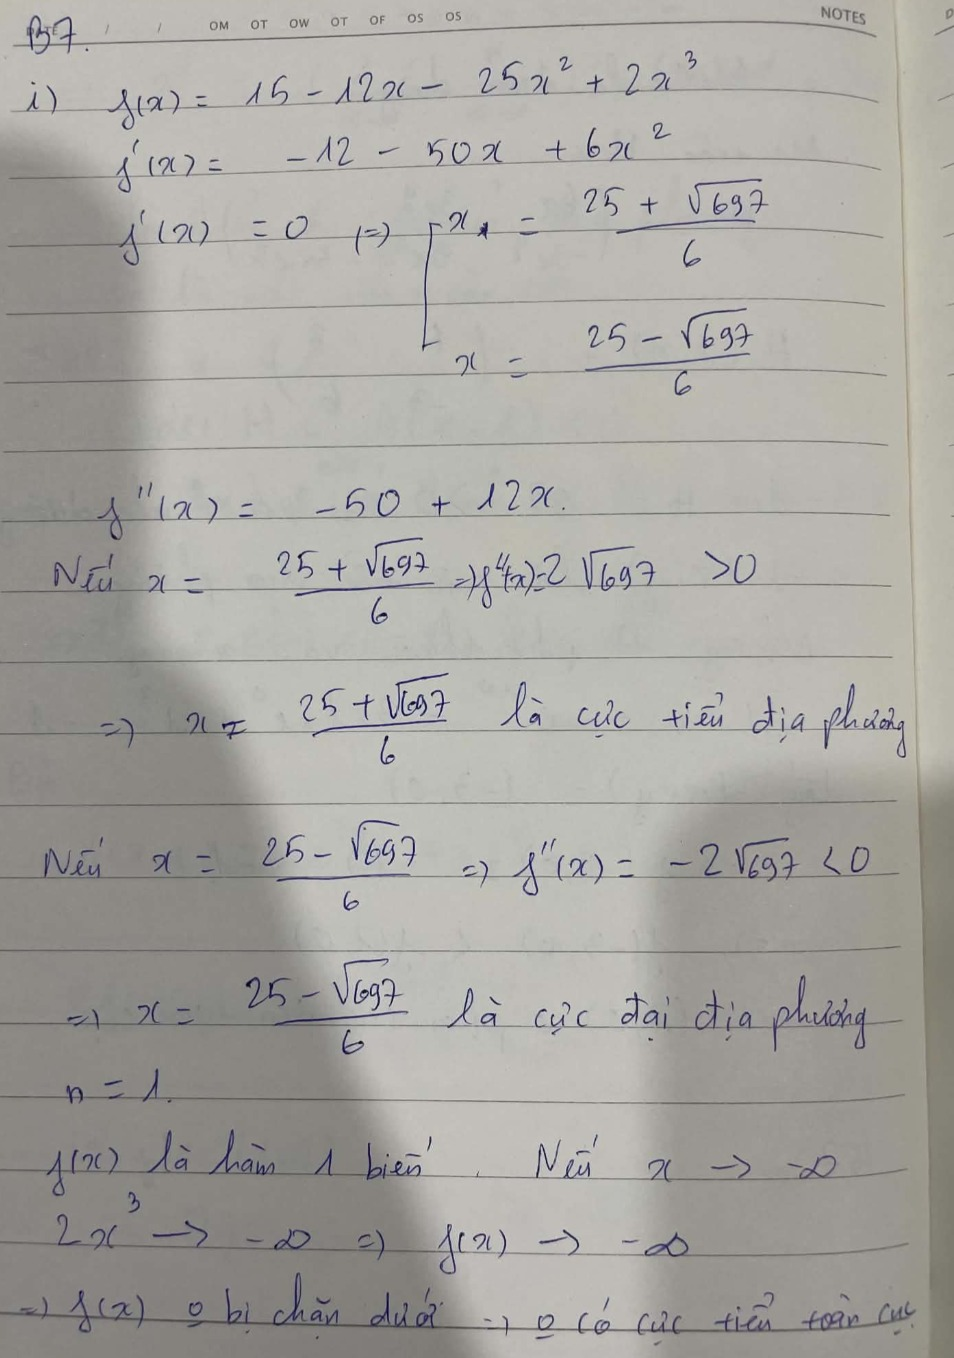
\includegraphics[width=.98\textwidth,height=.82\textheight,keepaspectratio]{bai_lam_them_1_assets/page-067.jpg}\end{center}
\clearpage
\phantomsection\label{src:068}
\noindent\textbf{Ảnh nguồn 068}\par\medskip
\begin{center}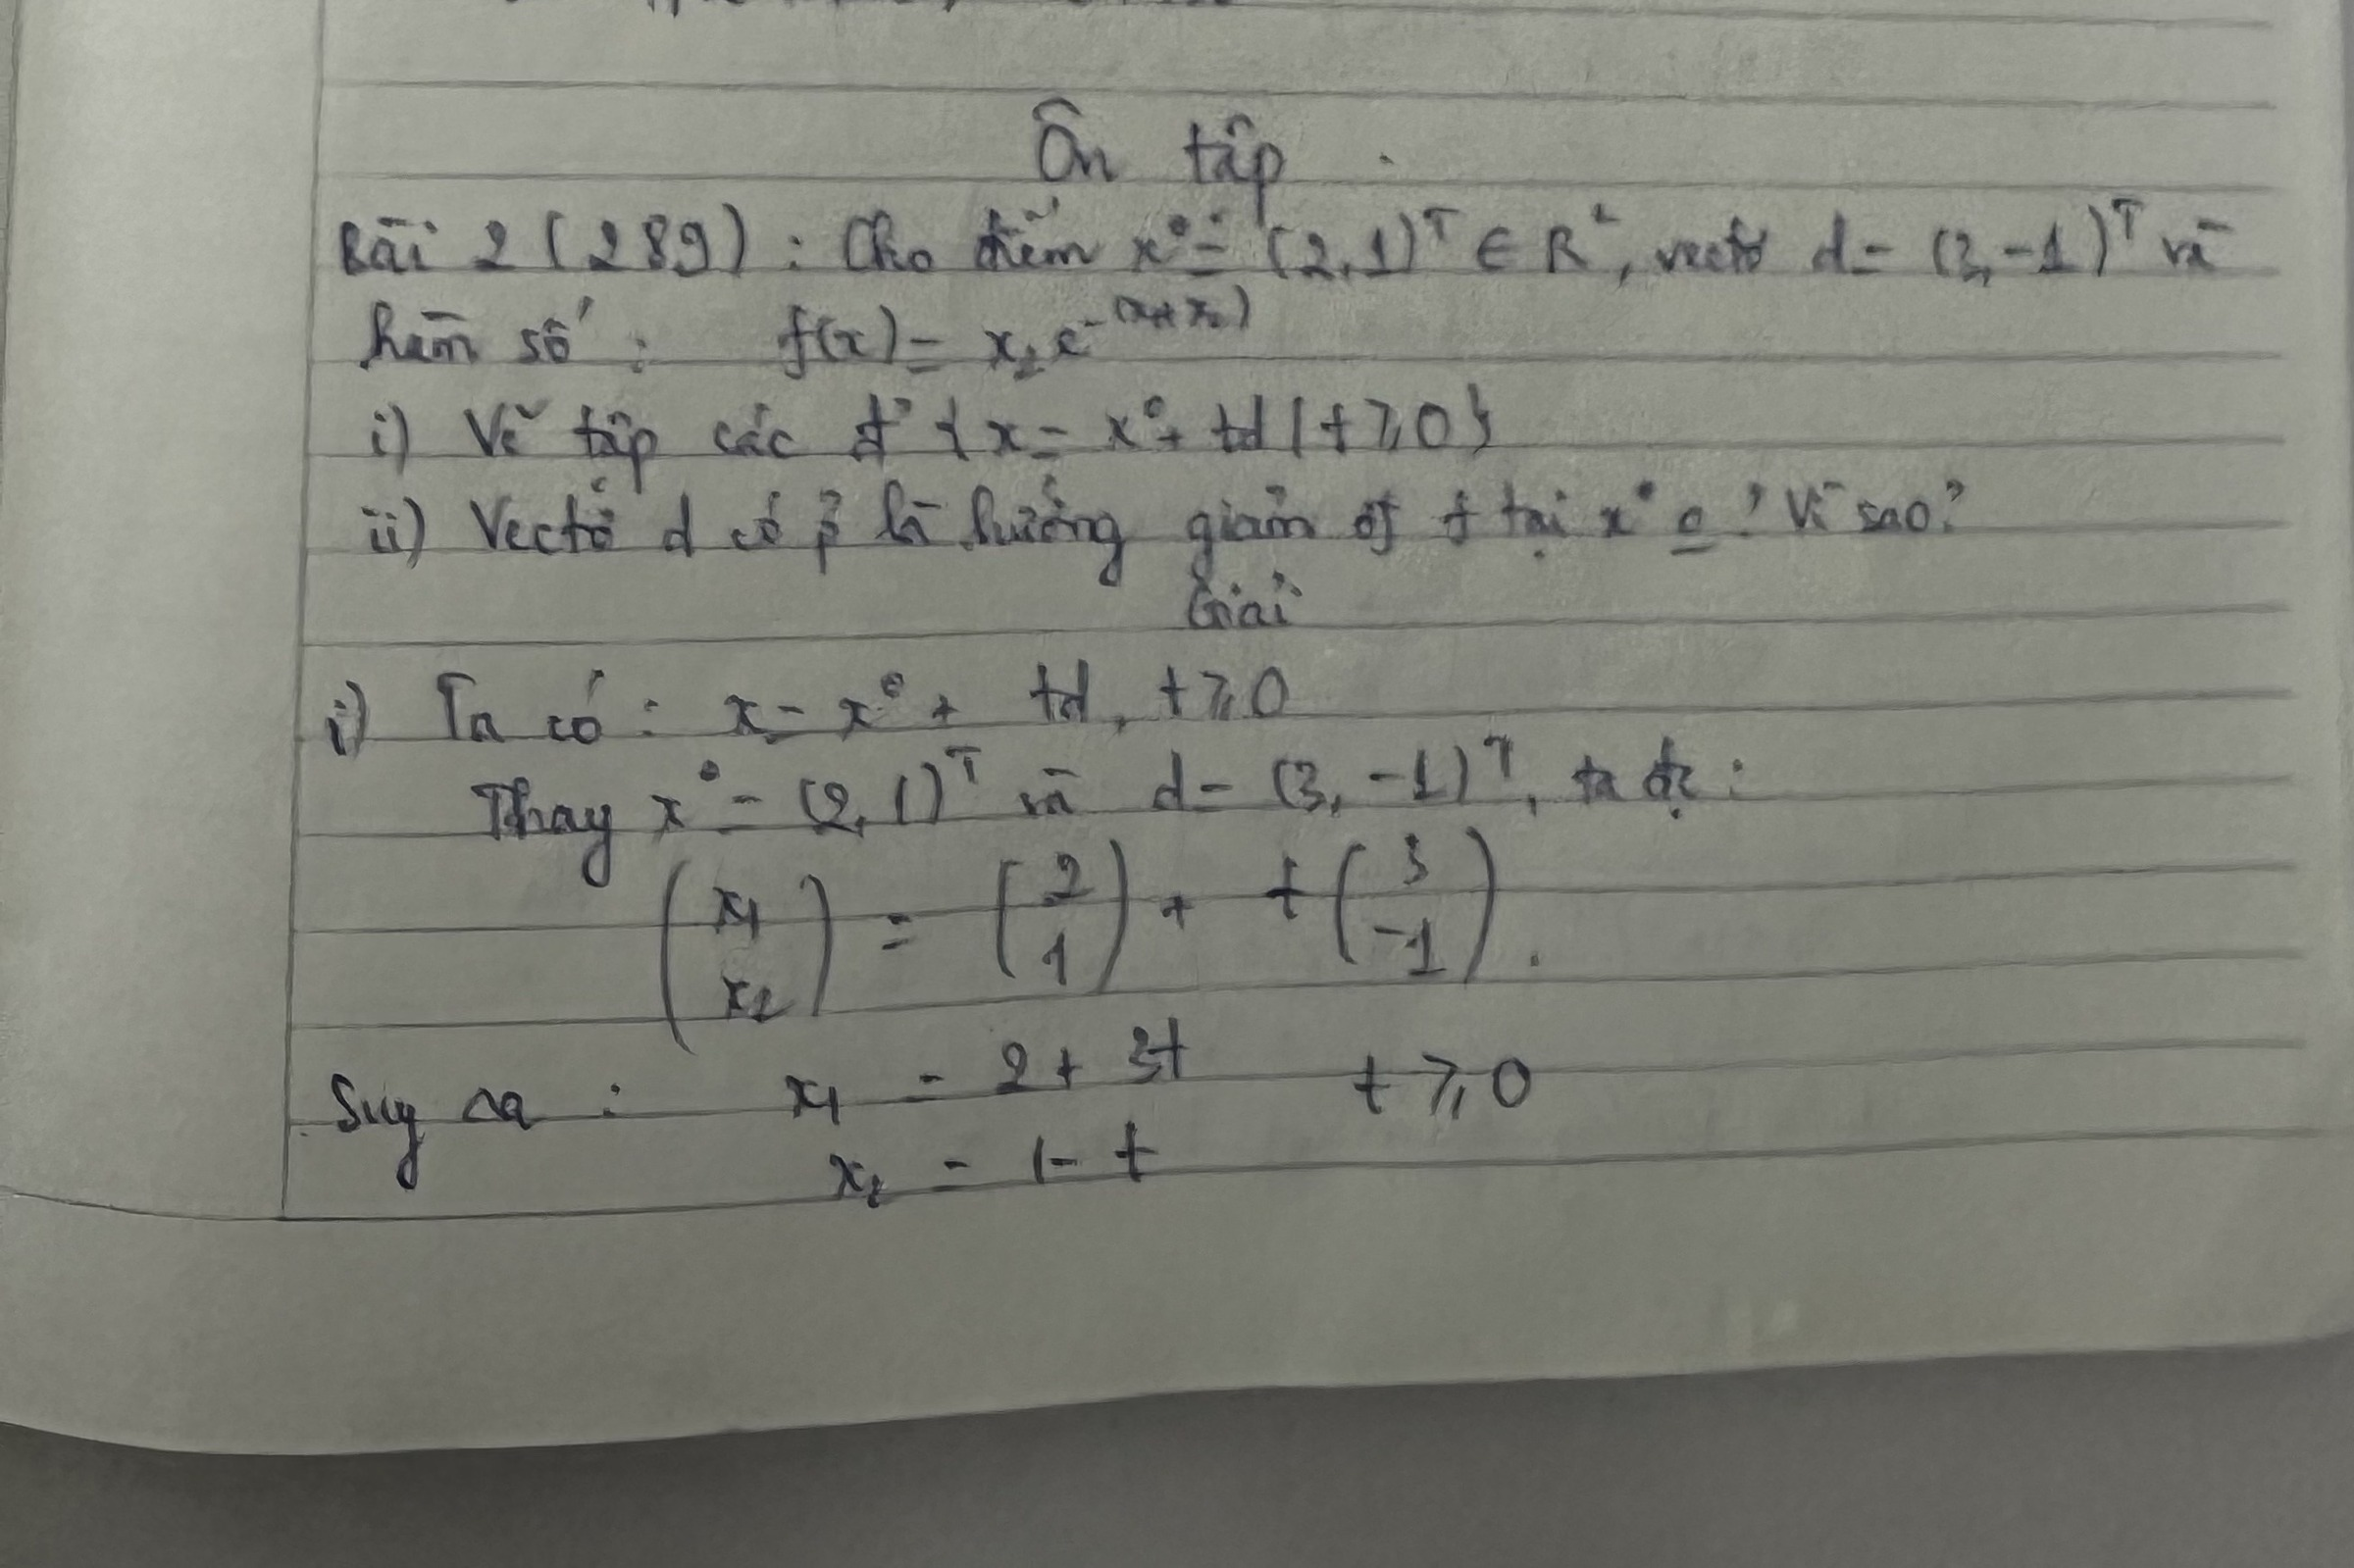
\includegraphics[width=.98\textwidth,height=.82\textheight,keepaspectratio]{bai_lam_them_1_assets/page-068.jpg}\end{center}
\clearpage
\phantomsection\label{src:069}
\noindent\textbf{Ảnh nguồn 069}\par\medskip
\begin{center}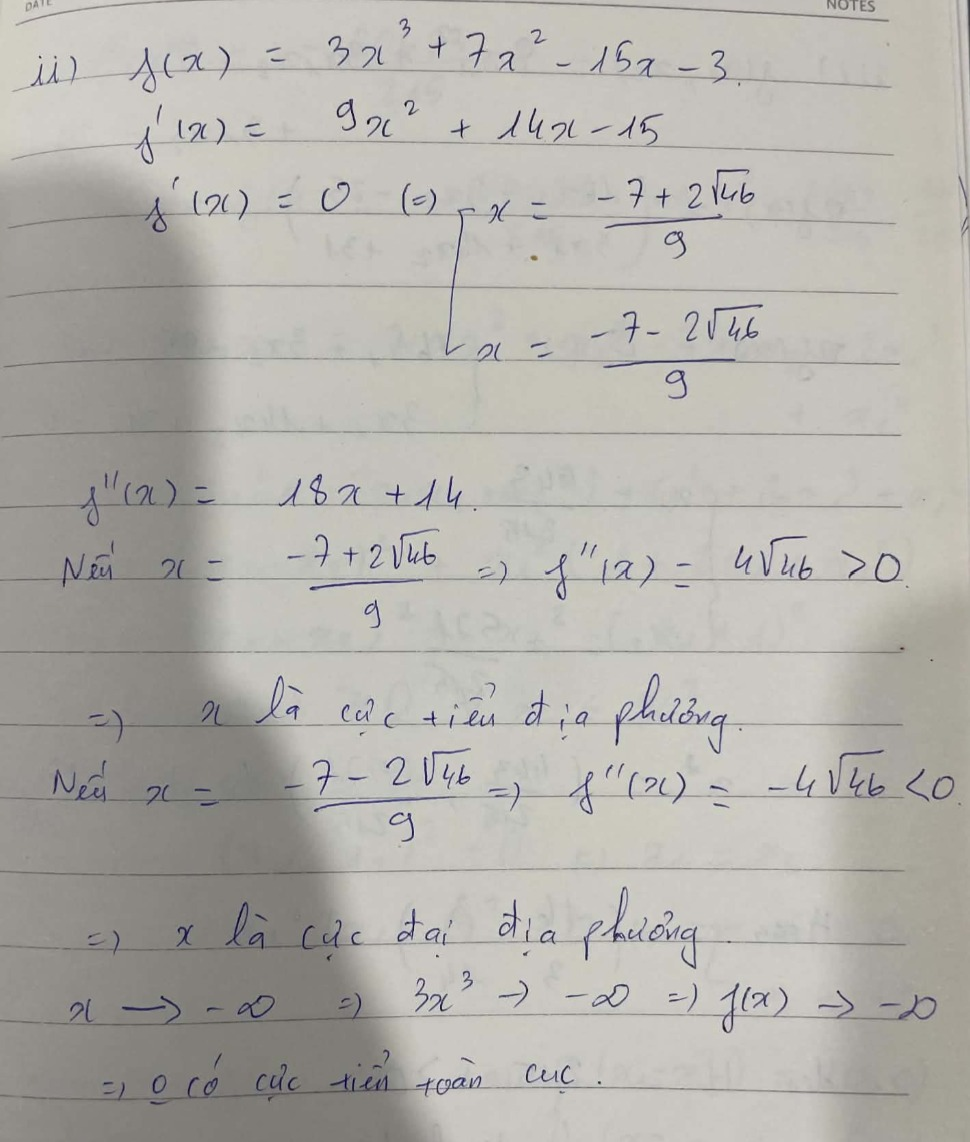
\includegraphics[width=.98\textwidth,height=.82\textheight,keepaspectratio]{bai_lam_them_1_assets/page-069.jpg}\end{center}
\clearpage
\phantomsection\label{src:070}
\noindent\textbf{Ảnh nguồn 070}\par\medskip
\begin{center}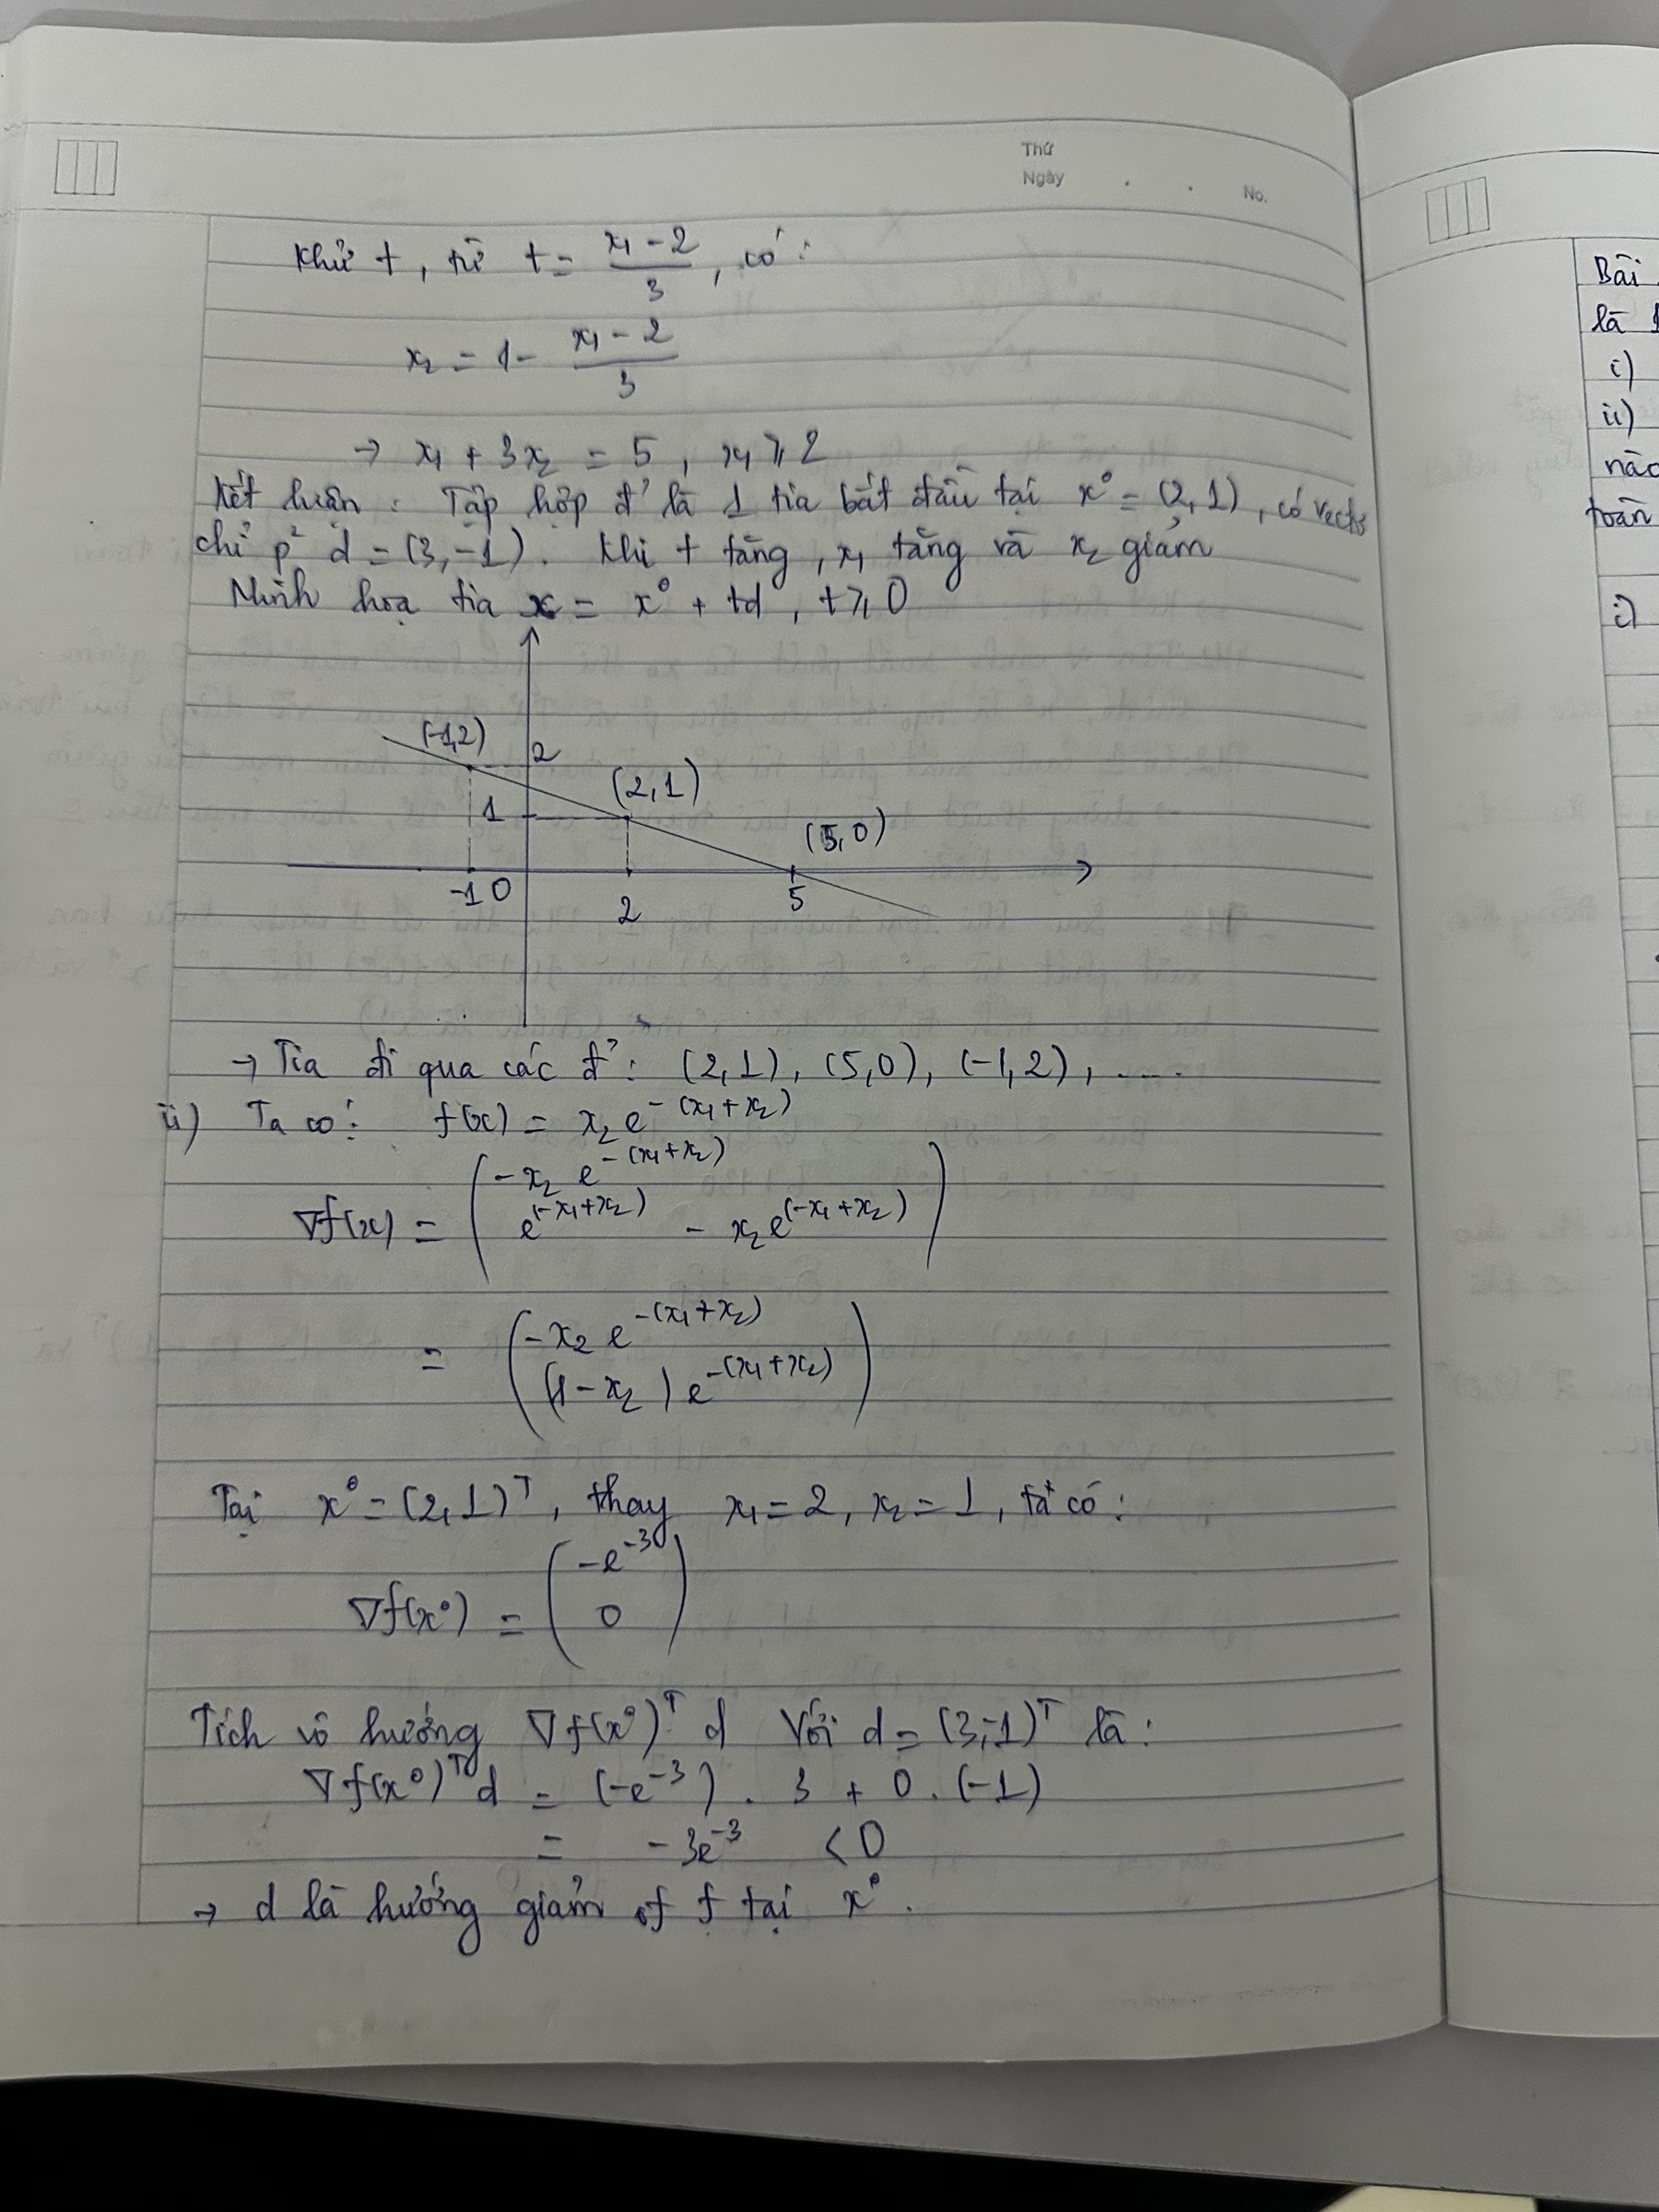
\includegraphics[width=.98\textwidth,height=.82\textheight,keepaspectratio]{bai_lam_them_1_assets/page-070.jpg}\end{center}
\clearpage
\phantomsection\label{src:071}
\noindent\textbf{Ảnh nguồn 071}\par\medskip
\begin{center}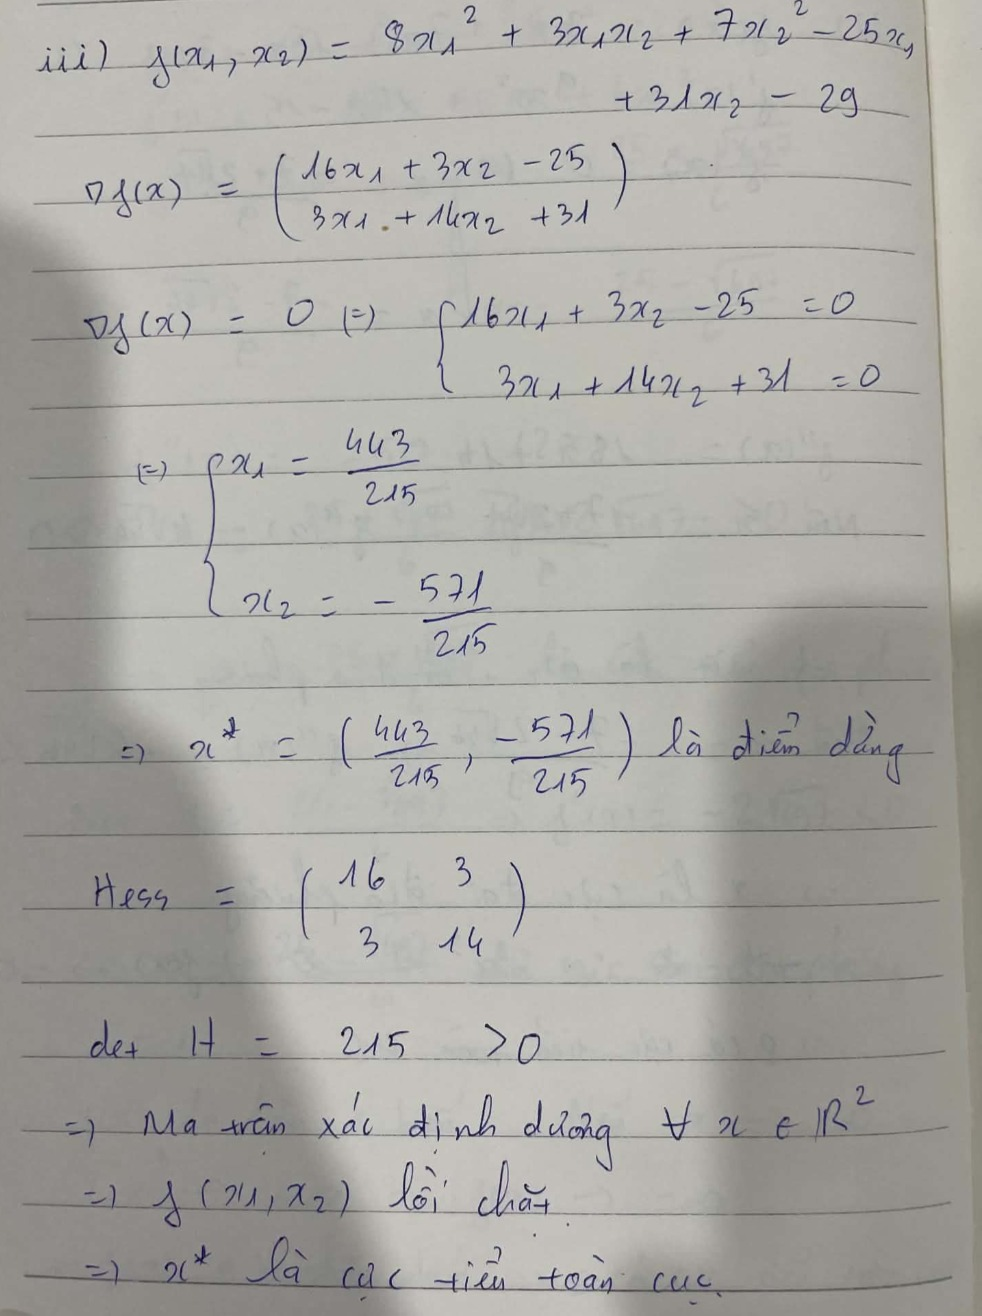
\includegraphics[width=.98\textwidth,height=.82\textheight,keepaspectratio]{bai_lam_them_1_assets/page-071.jpg}\end{center}
\clearpage
\phantomsection\label{src:072}
\noindent\textbf{Ảnh nguồn 072}\par\medskip
\begin{center}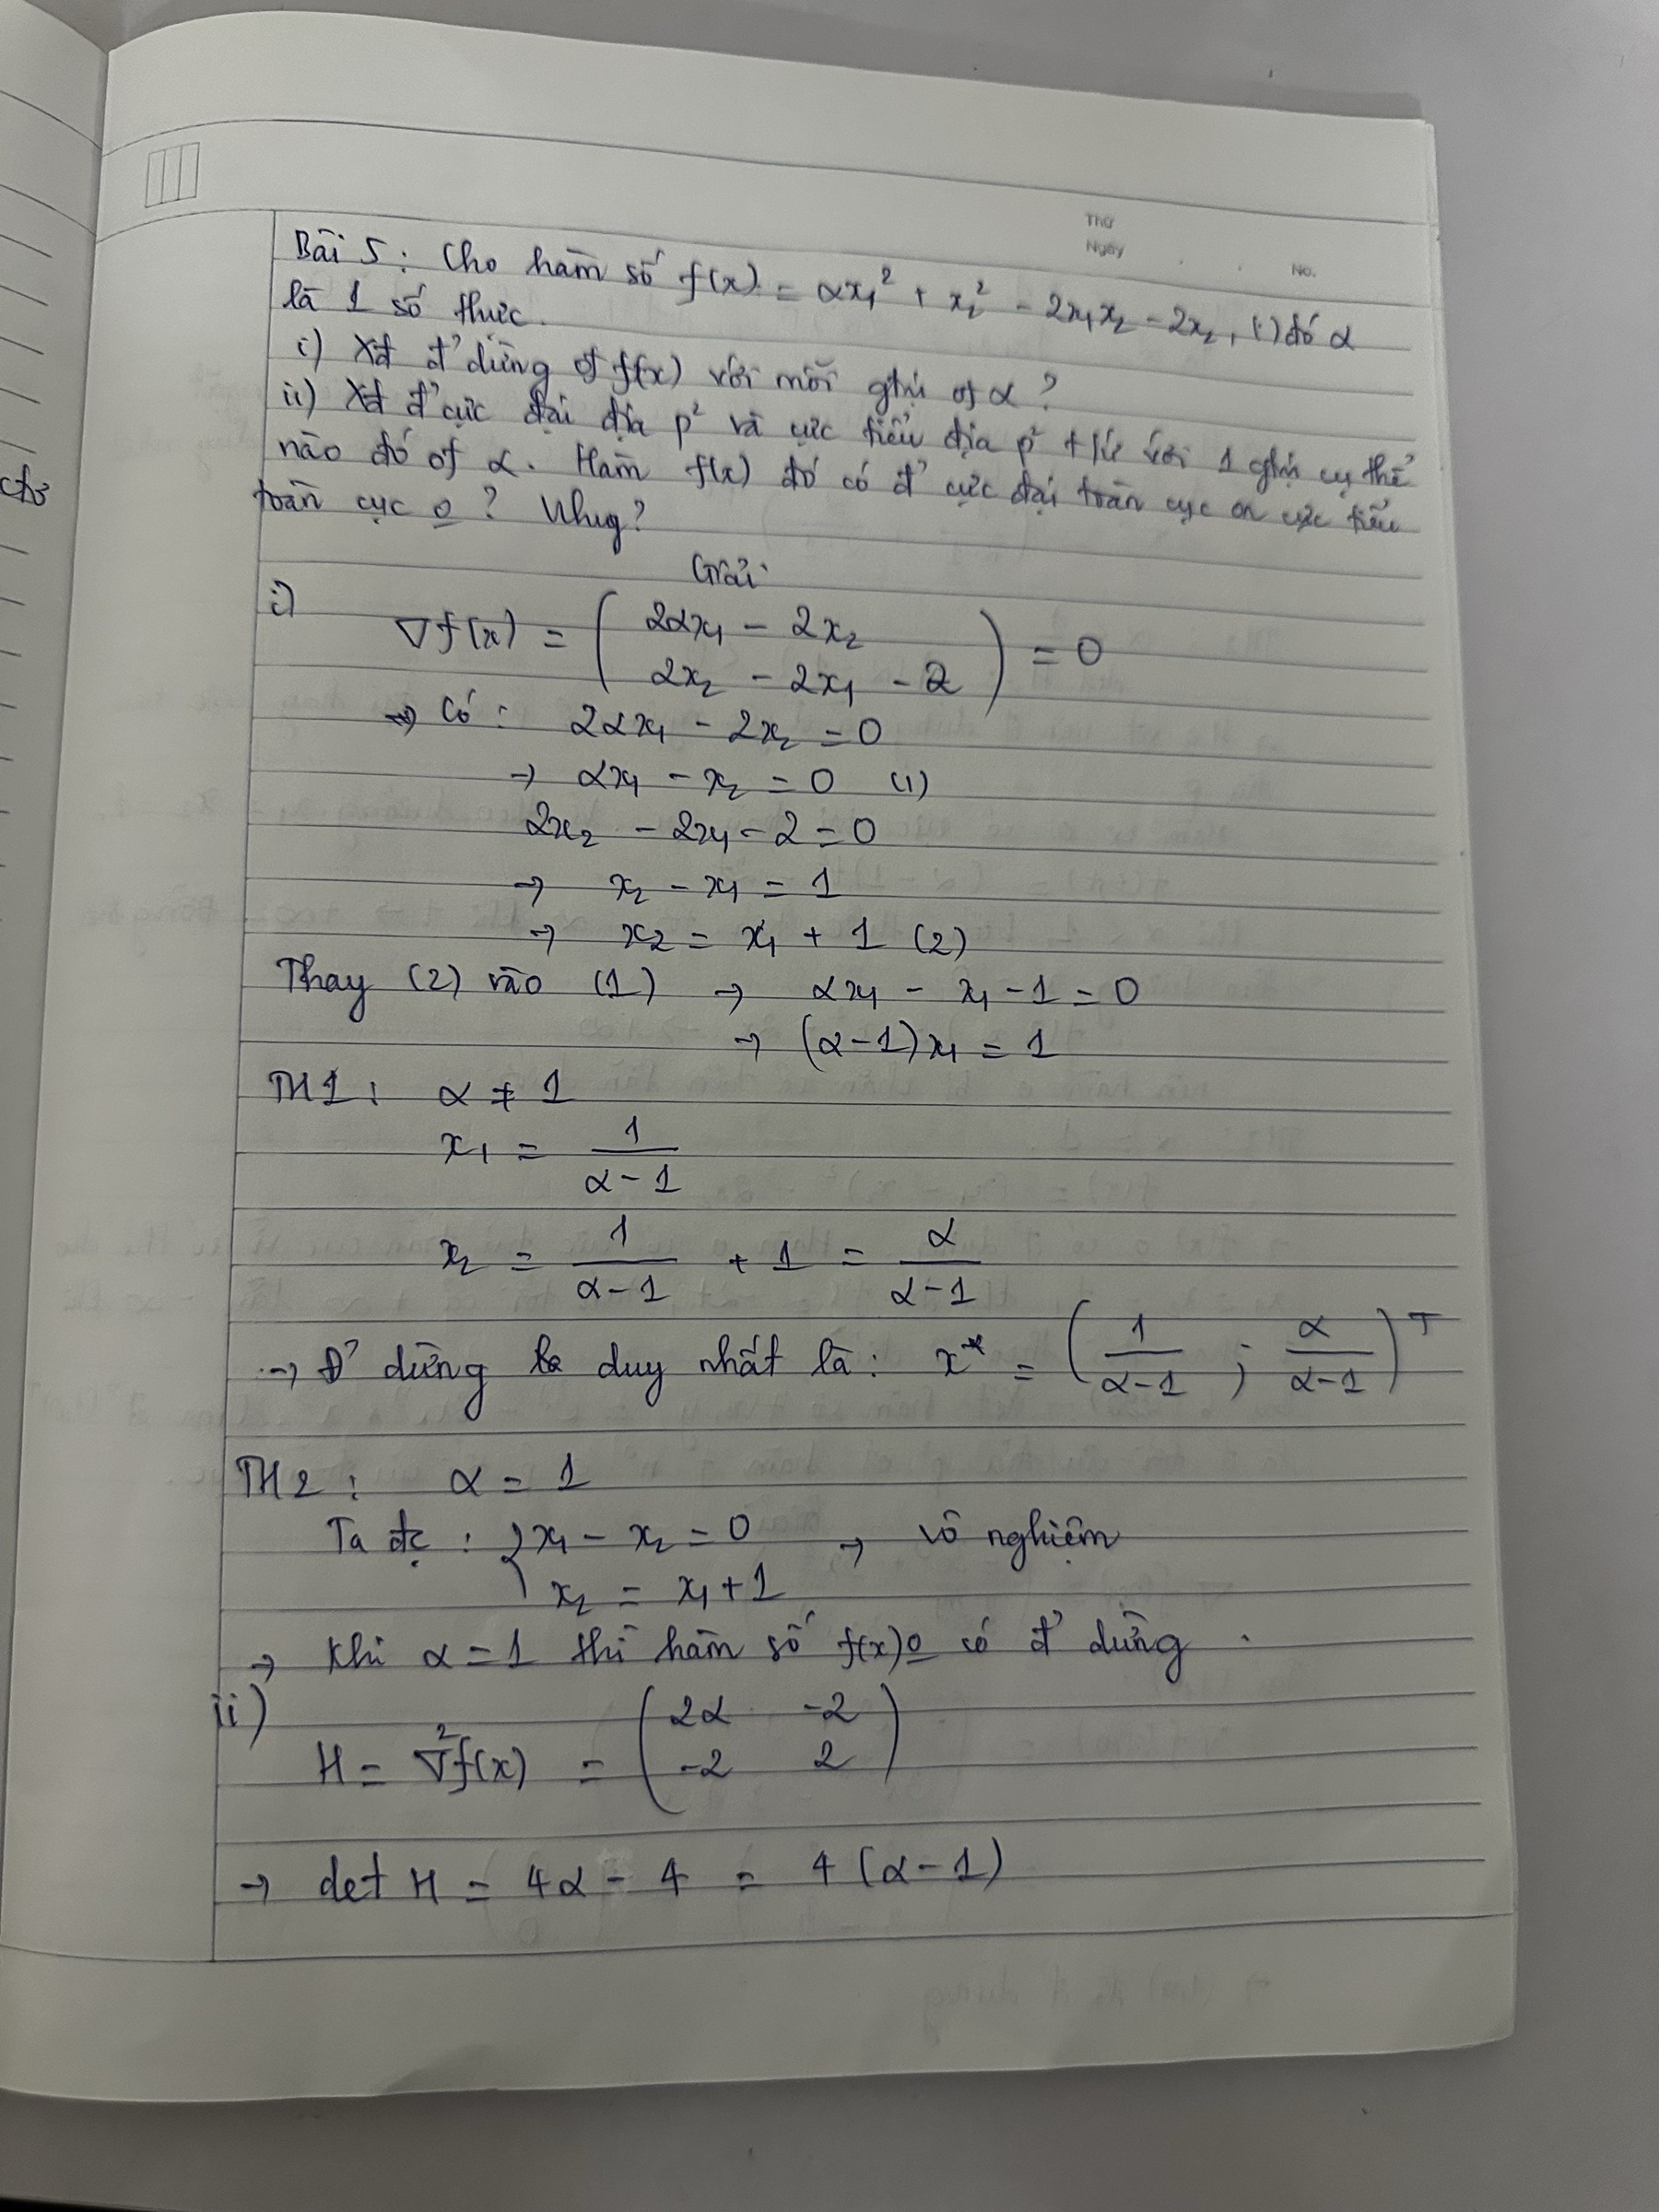
\includegraphics[width=.98\textwidth,height=.82\textheight,keepaspectratio]{bai_lam_them_1_assets/page-072.jpg}\end{center}
\clearpage
\phantomsection\label{src:073}
\noindent\textbf{Ảnh nguồn 073}\par\medskip
\begin{center}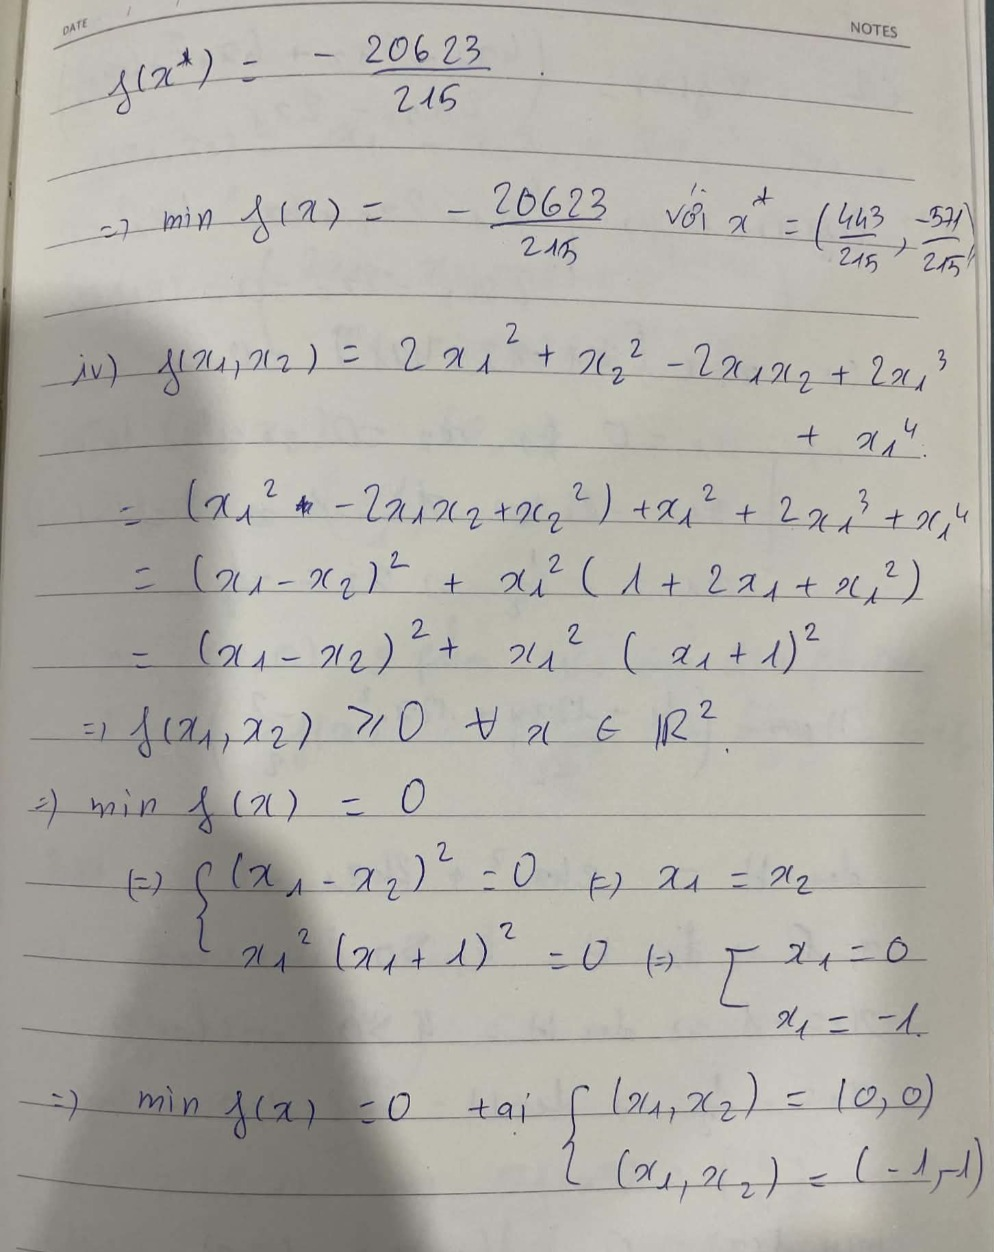
\includegraphics[width=.98\textwidth,height=.82\textheight,keepaspectratio]{bai_lam_them_1_assets/page-073.jpg}\end{center}
\clearpage
\phantomsection\label{src:074}
\noindent\textbf{Ảnh nguồn 074}\par\medskip
\begin{center}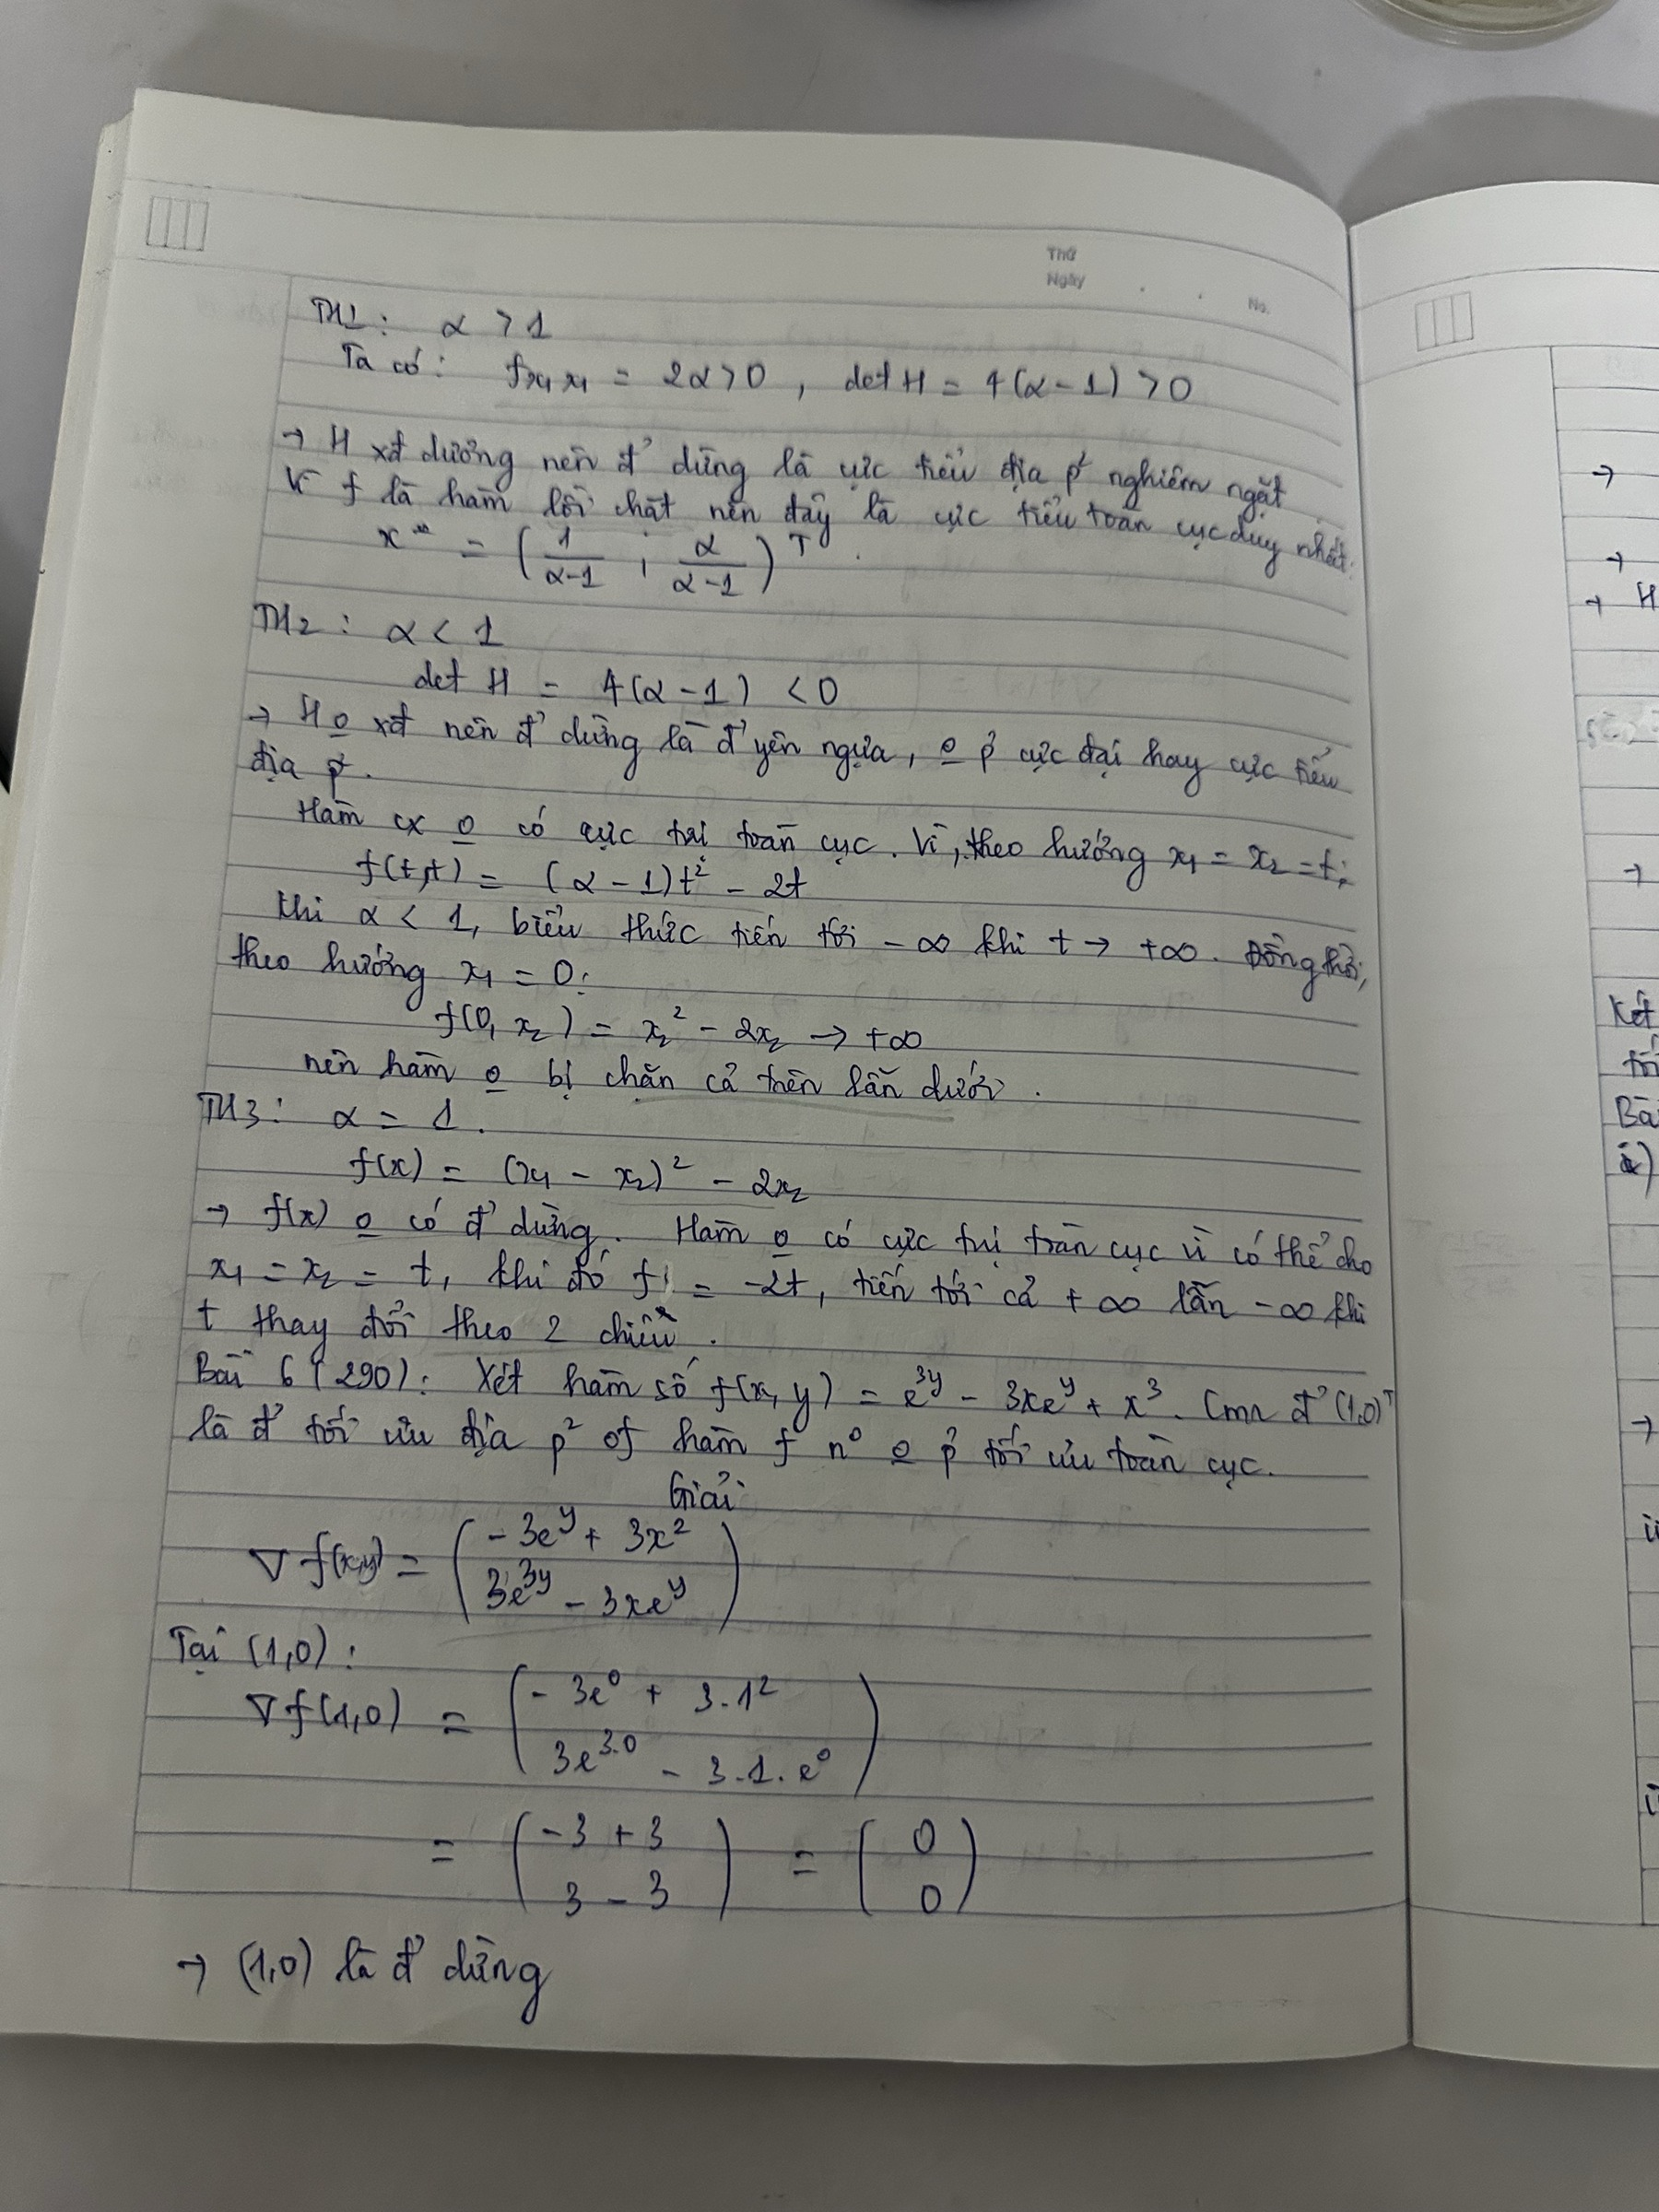
\includegraphics[width=.98\textwidth,height=.82\textheight,keepaspectratio]{bai_lam_them_1_assets/page-074.jpg}\end{center}
\clearpage
\phantomsection\label{src:075}
\noindent\textbf{Ảnh nguồn 075}\par\medskip
\begin{center}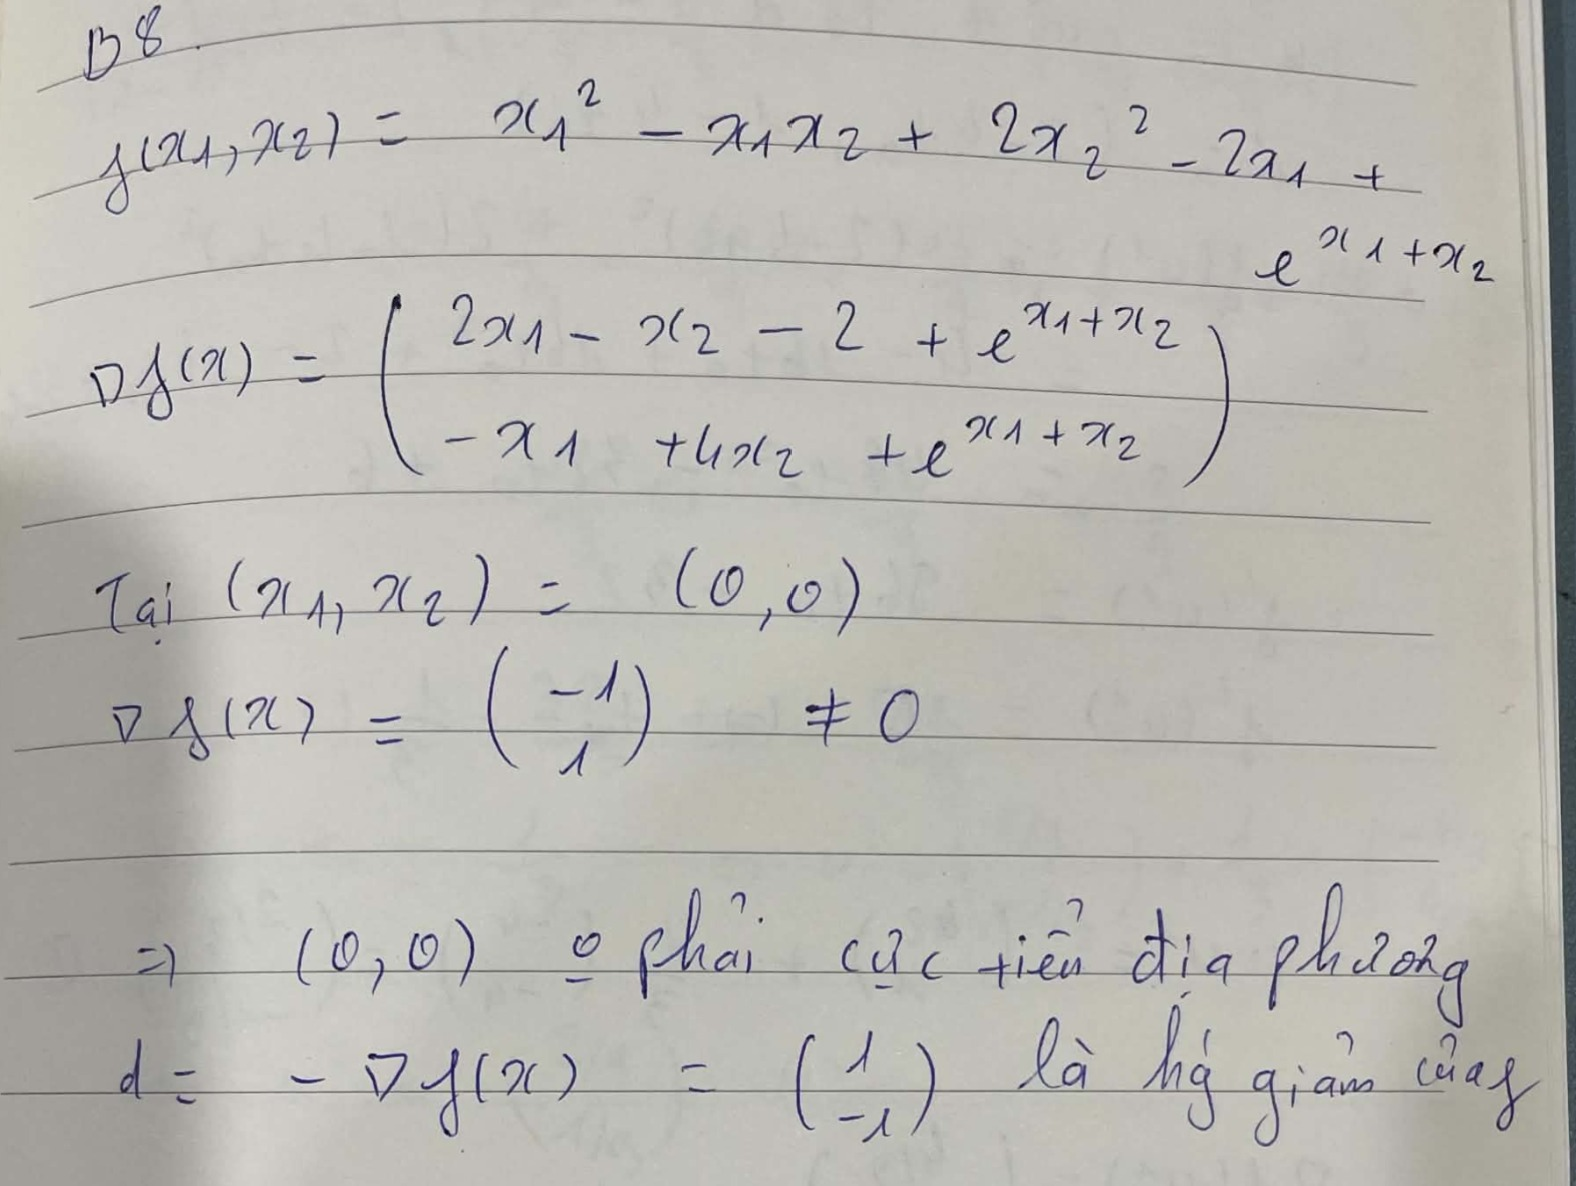
\includegraphics[width=.98\textwidth,height=.82\textheight,keepaspectratio]{bai_lam_them_1_assets/page-075.jpg}\end{center}
\clearpage
\phantomsection\label{src:076}
\noindent\textbf{Ảnh nguồn 076}\par\medskip
\begin{center}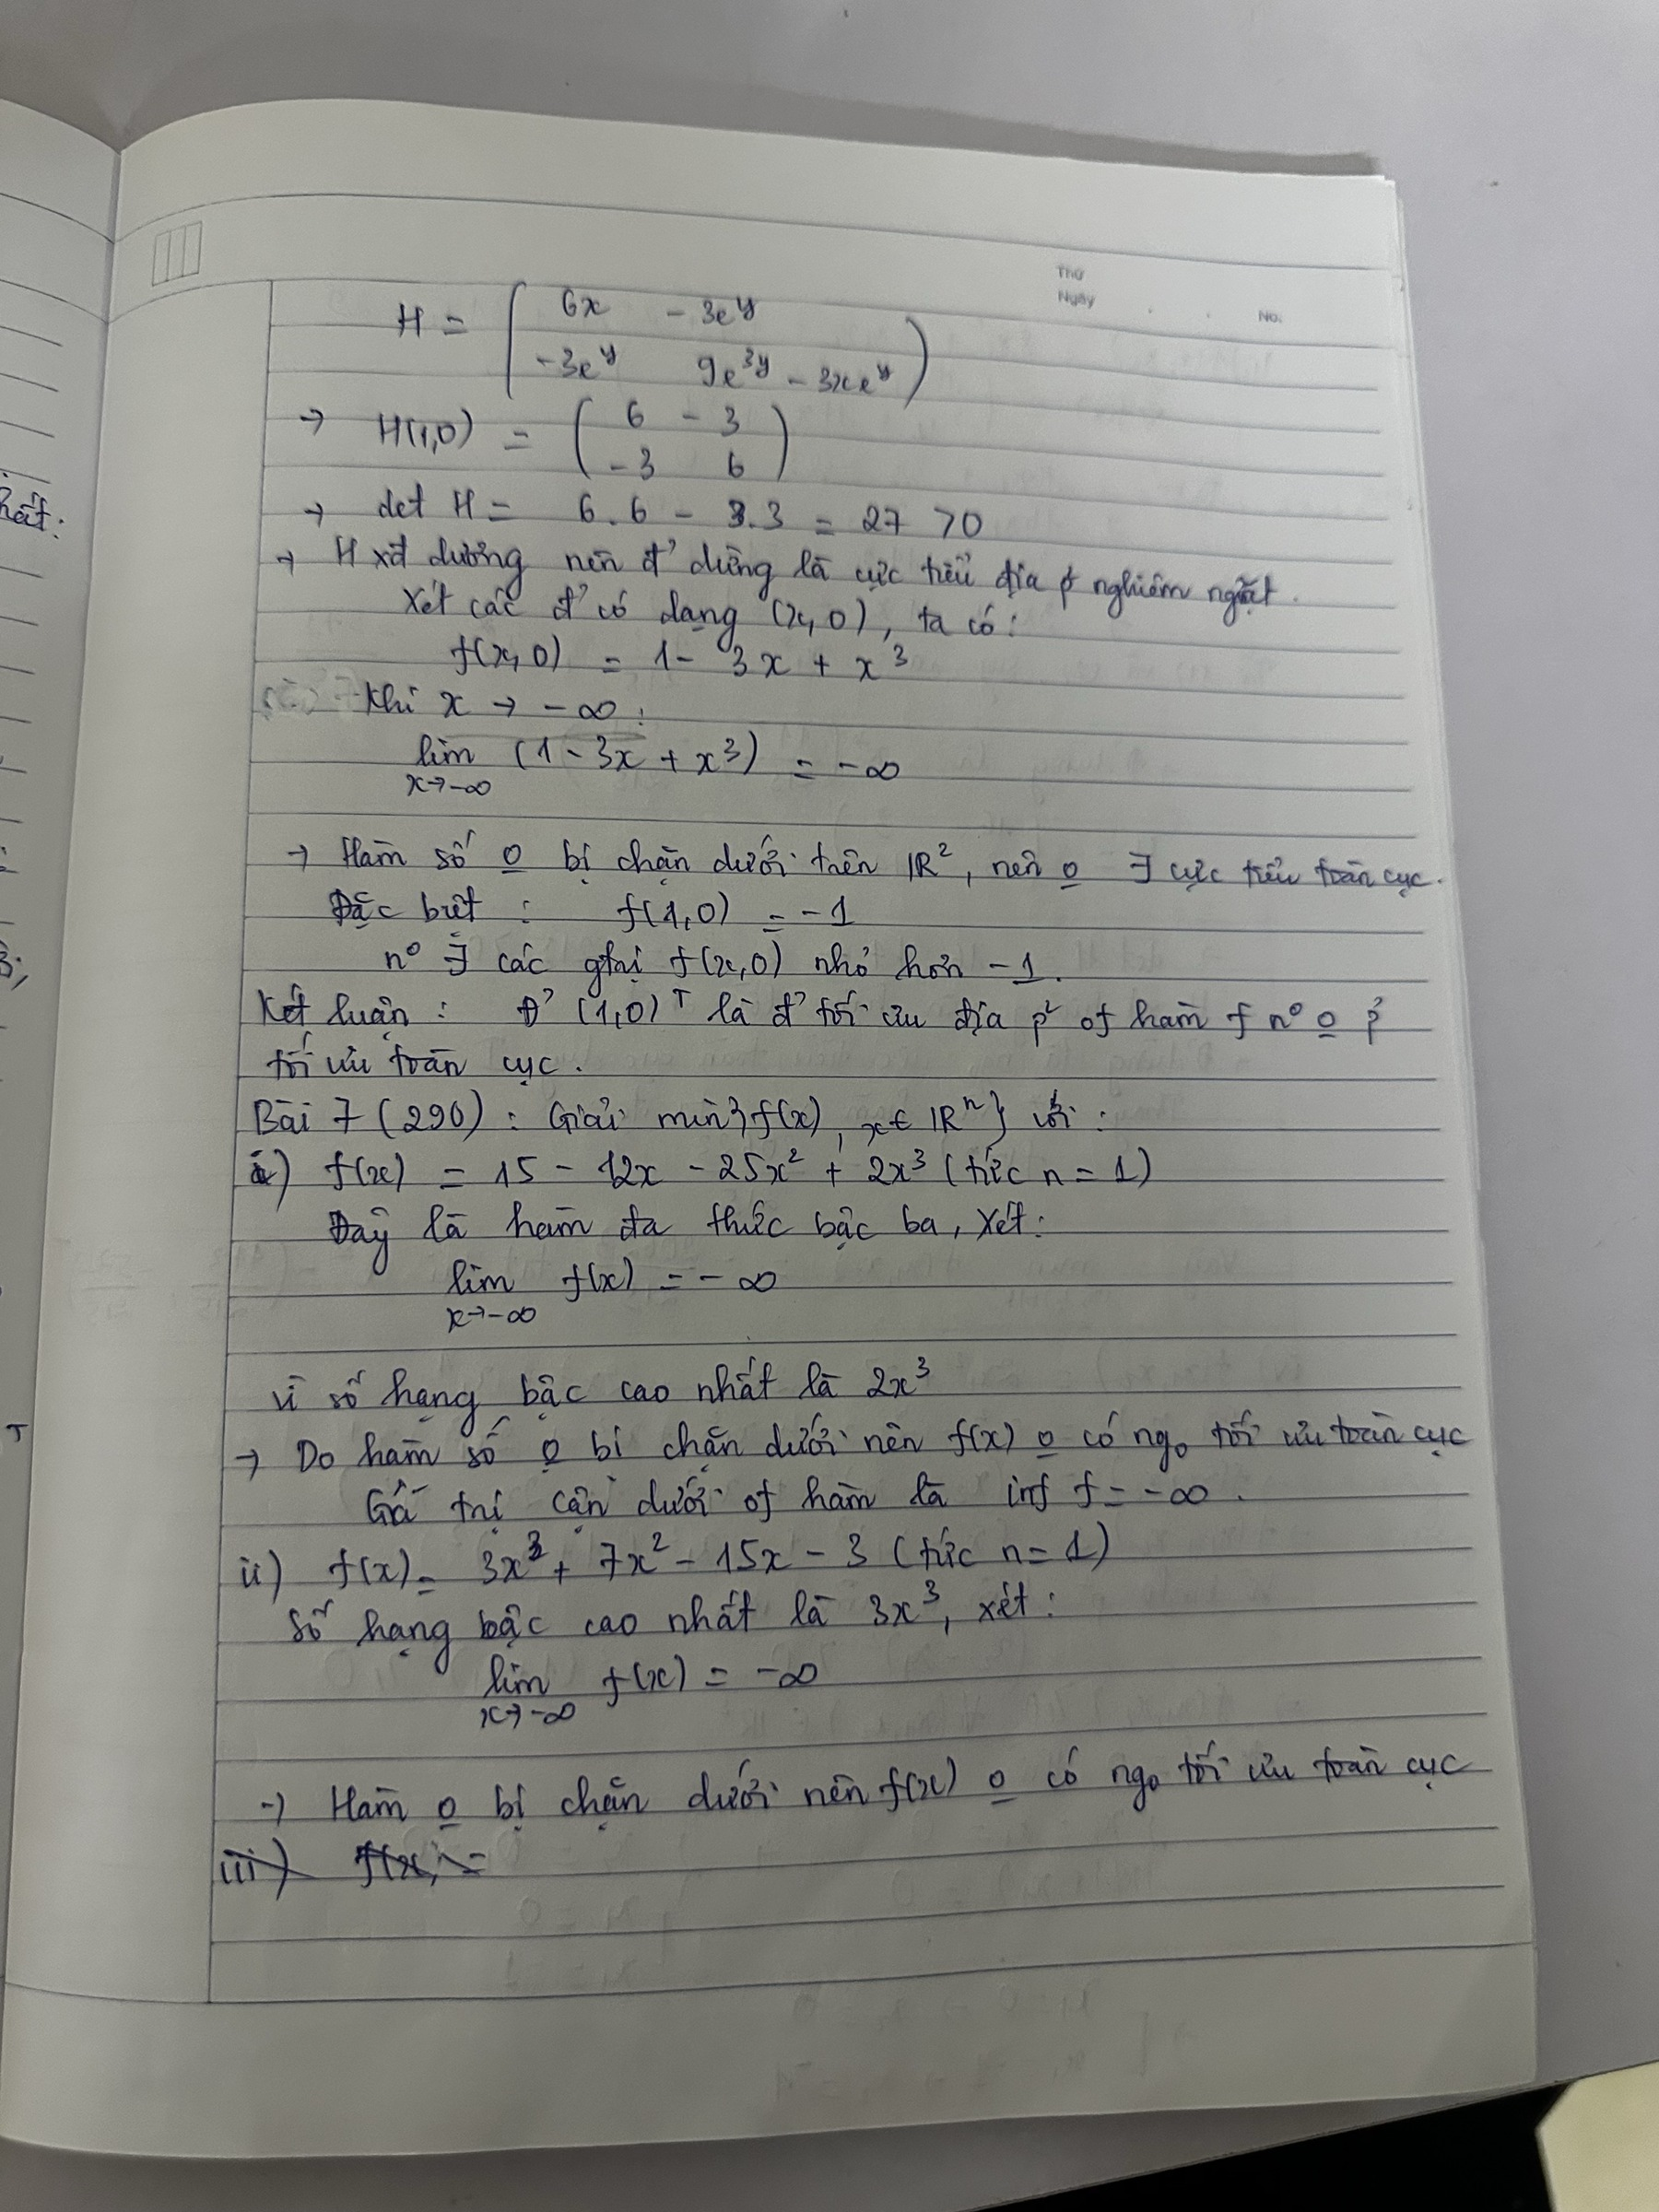
\includegraphics[width=.98\textwidth,height=.82\textheight,keepaspectratio]{bai_lam_them_1_assets/page-076.jpg}\end{center}
\clearpage
\phantomsection\label{src:077}
\noindent\textbf{Ảnh nguồn 077}\par\medskip
\begin{center}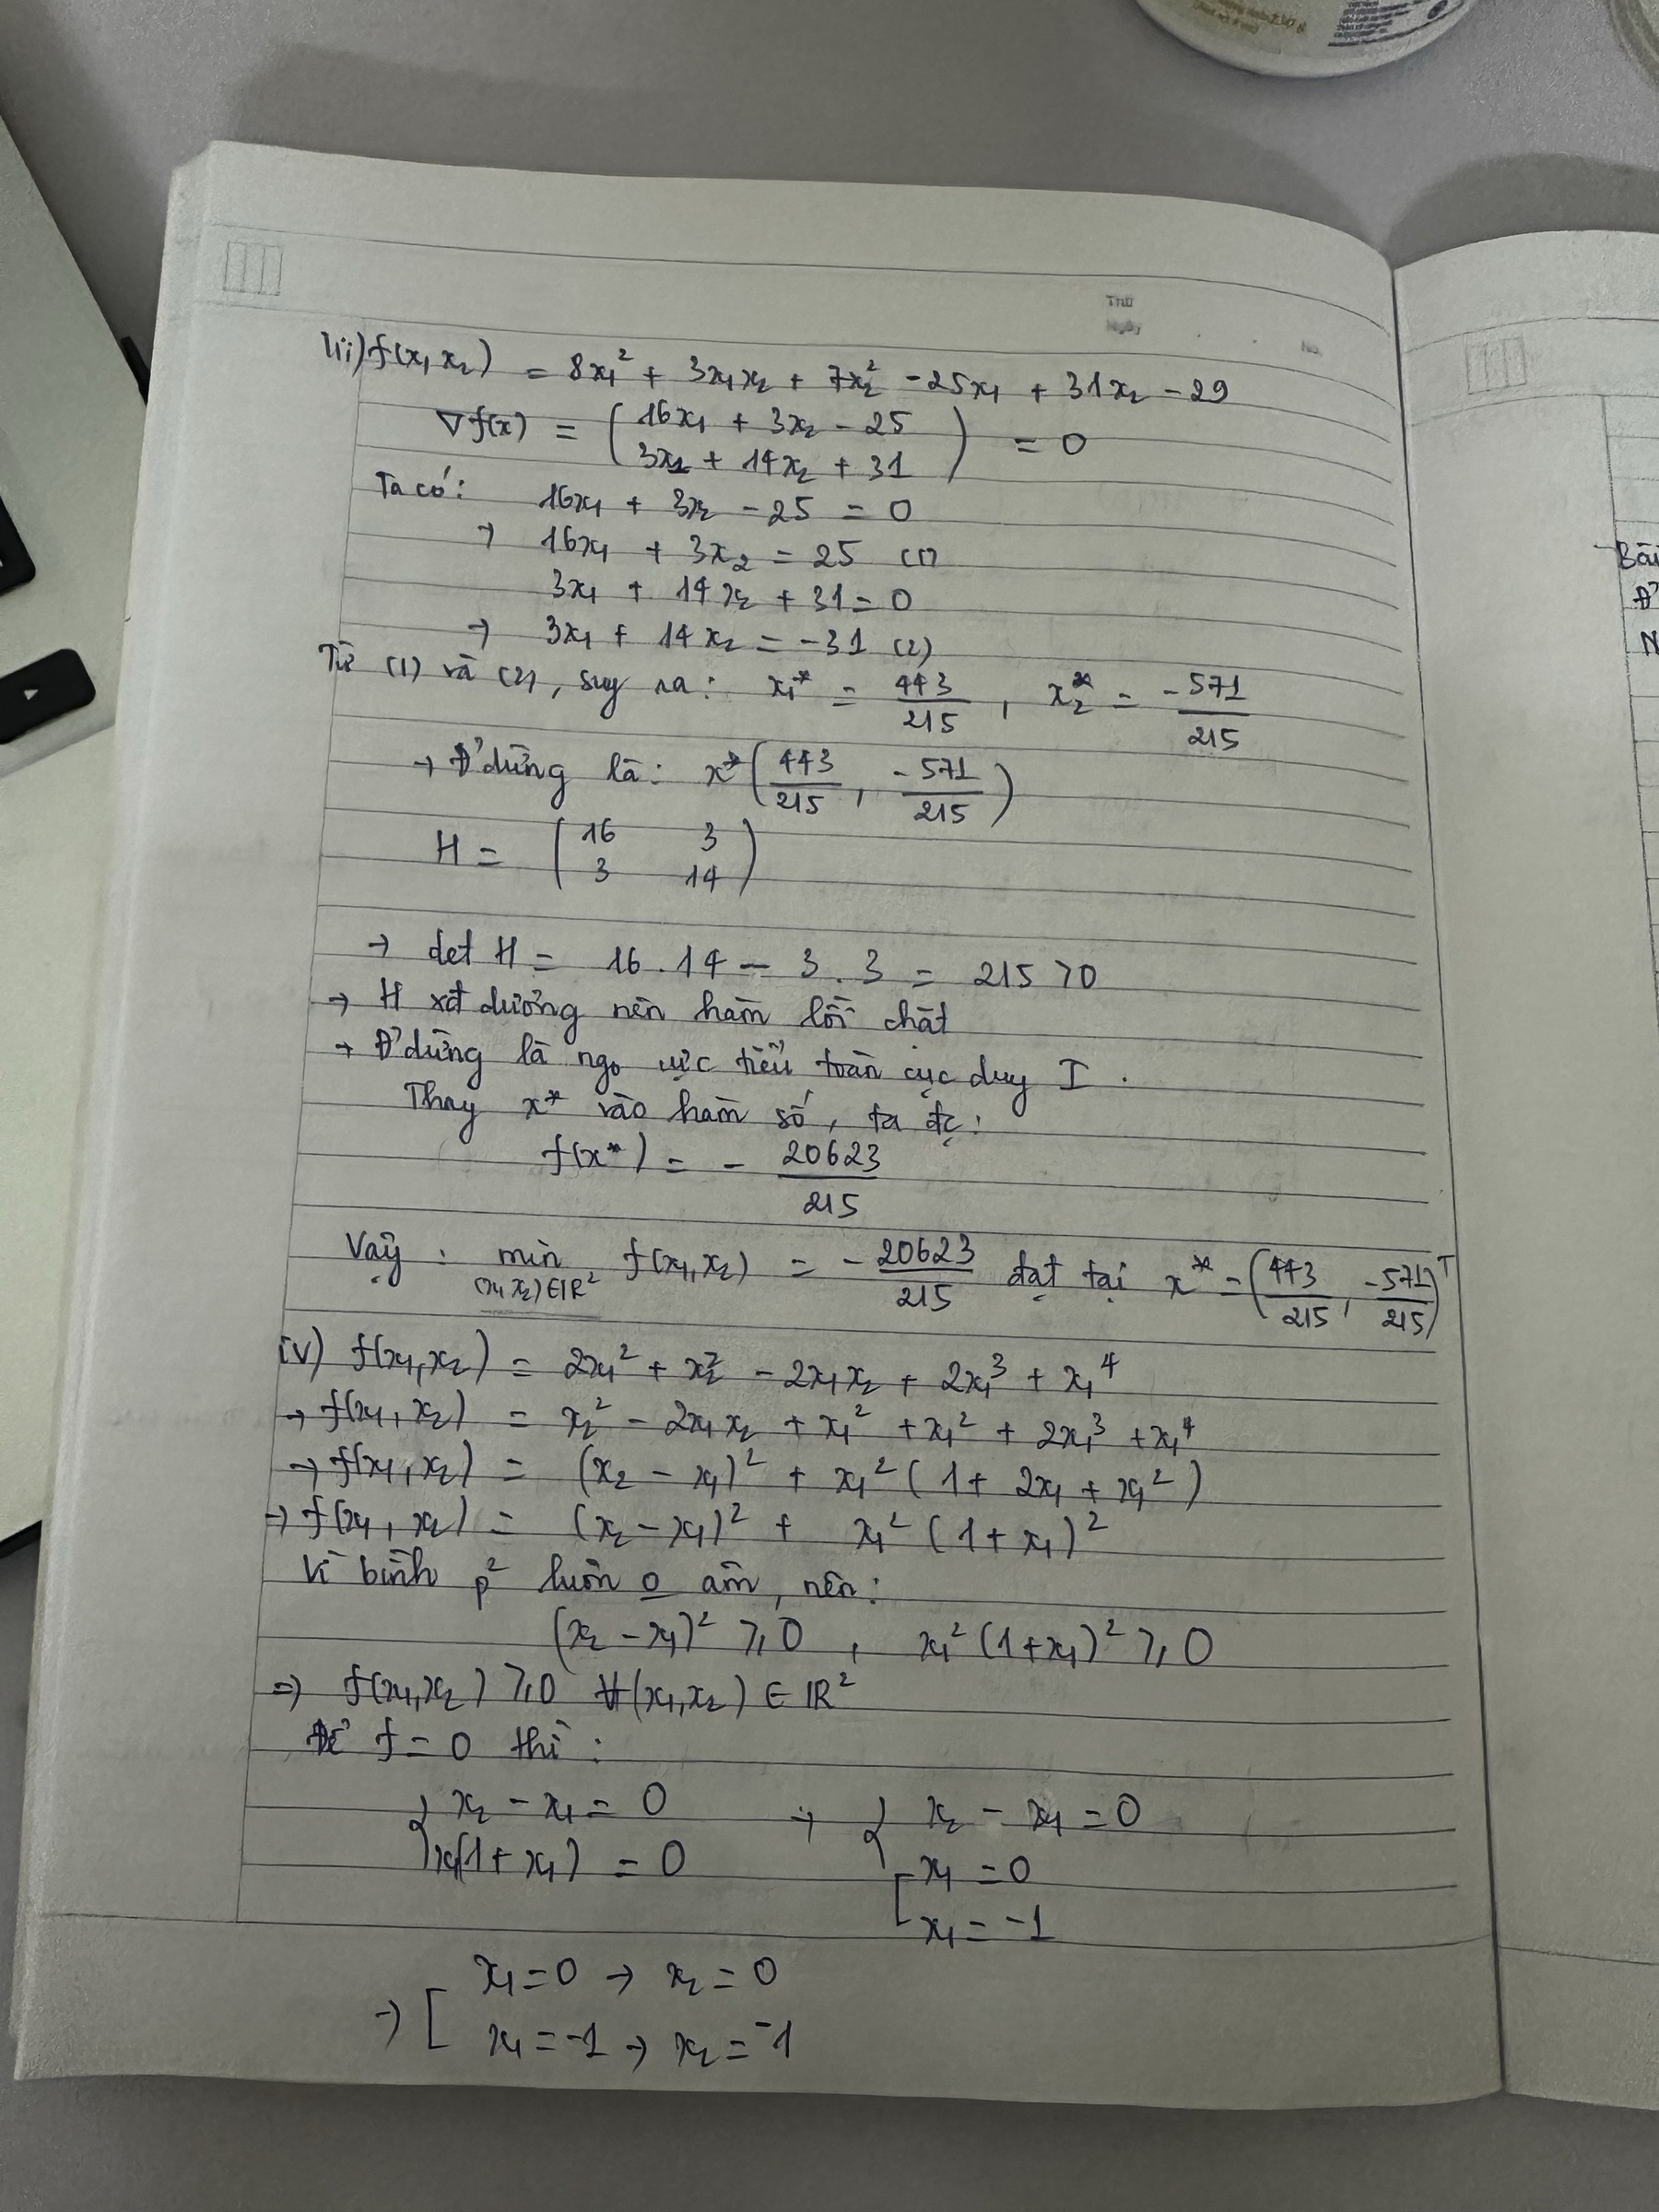
\includegraphics[width=.98\textwidth,height=.82\textheight,keepaspectratio]{bai_lam_them_1_assets/page-077.jpg}\end{center}
\clearpage
\phantomsection\label{src:078}
\noindent\textbf{Ảnh nguồn 078}\par\medskip
\begin{center}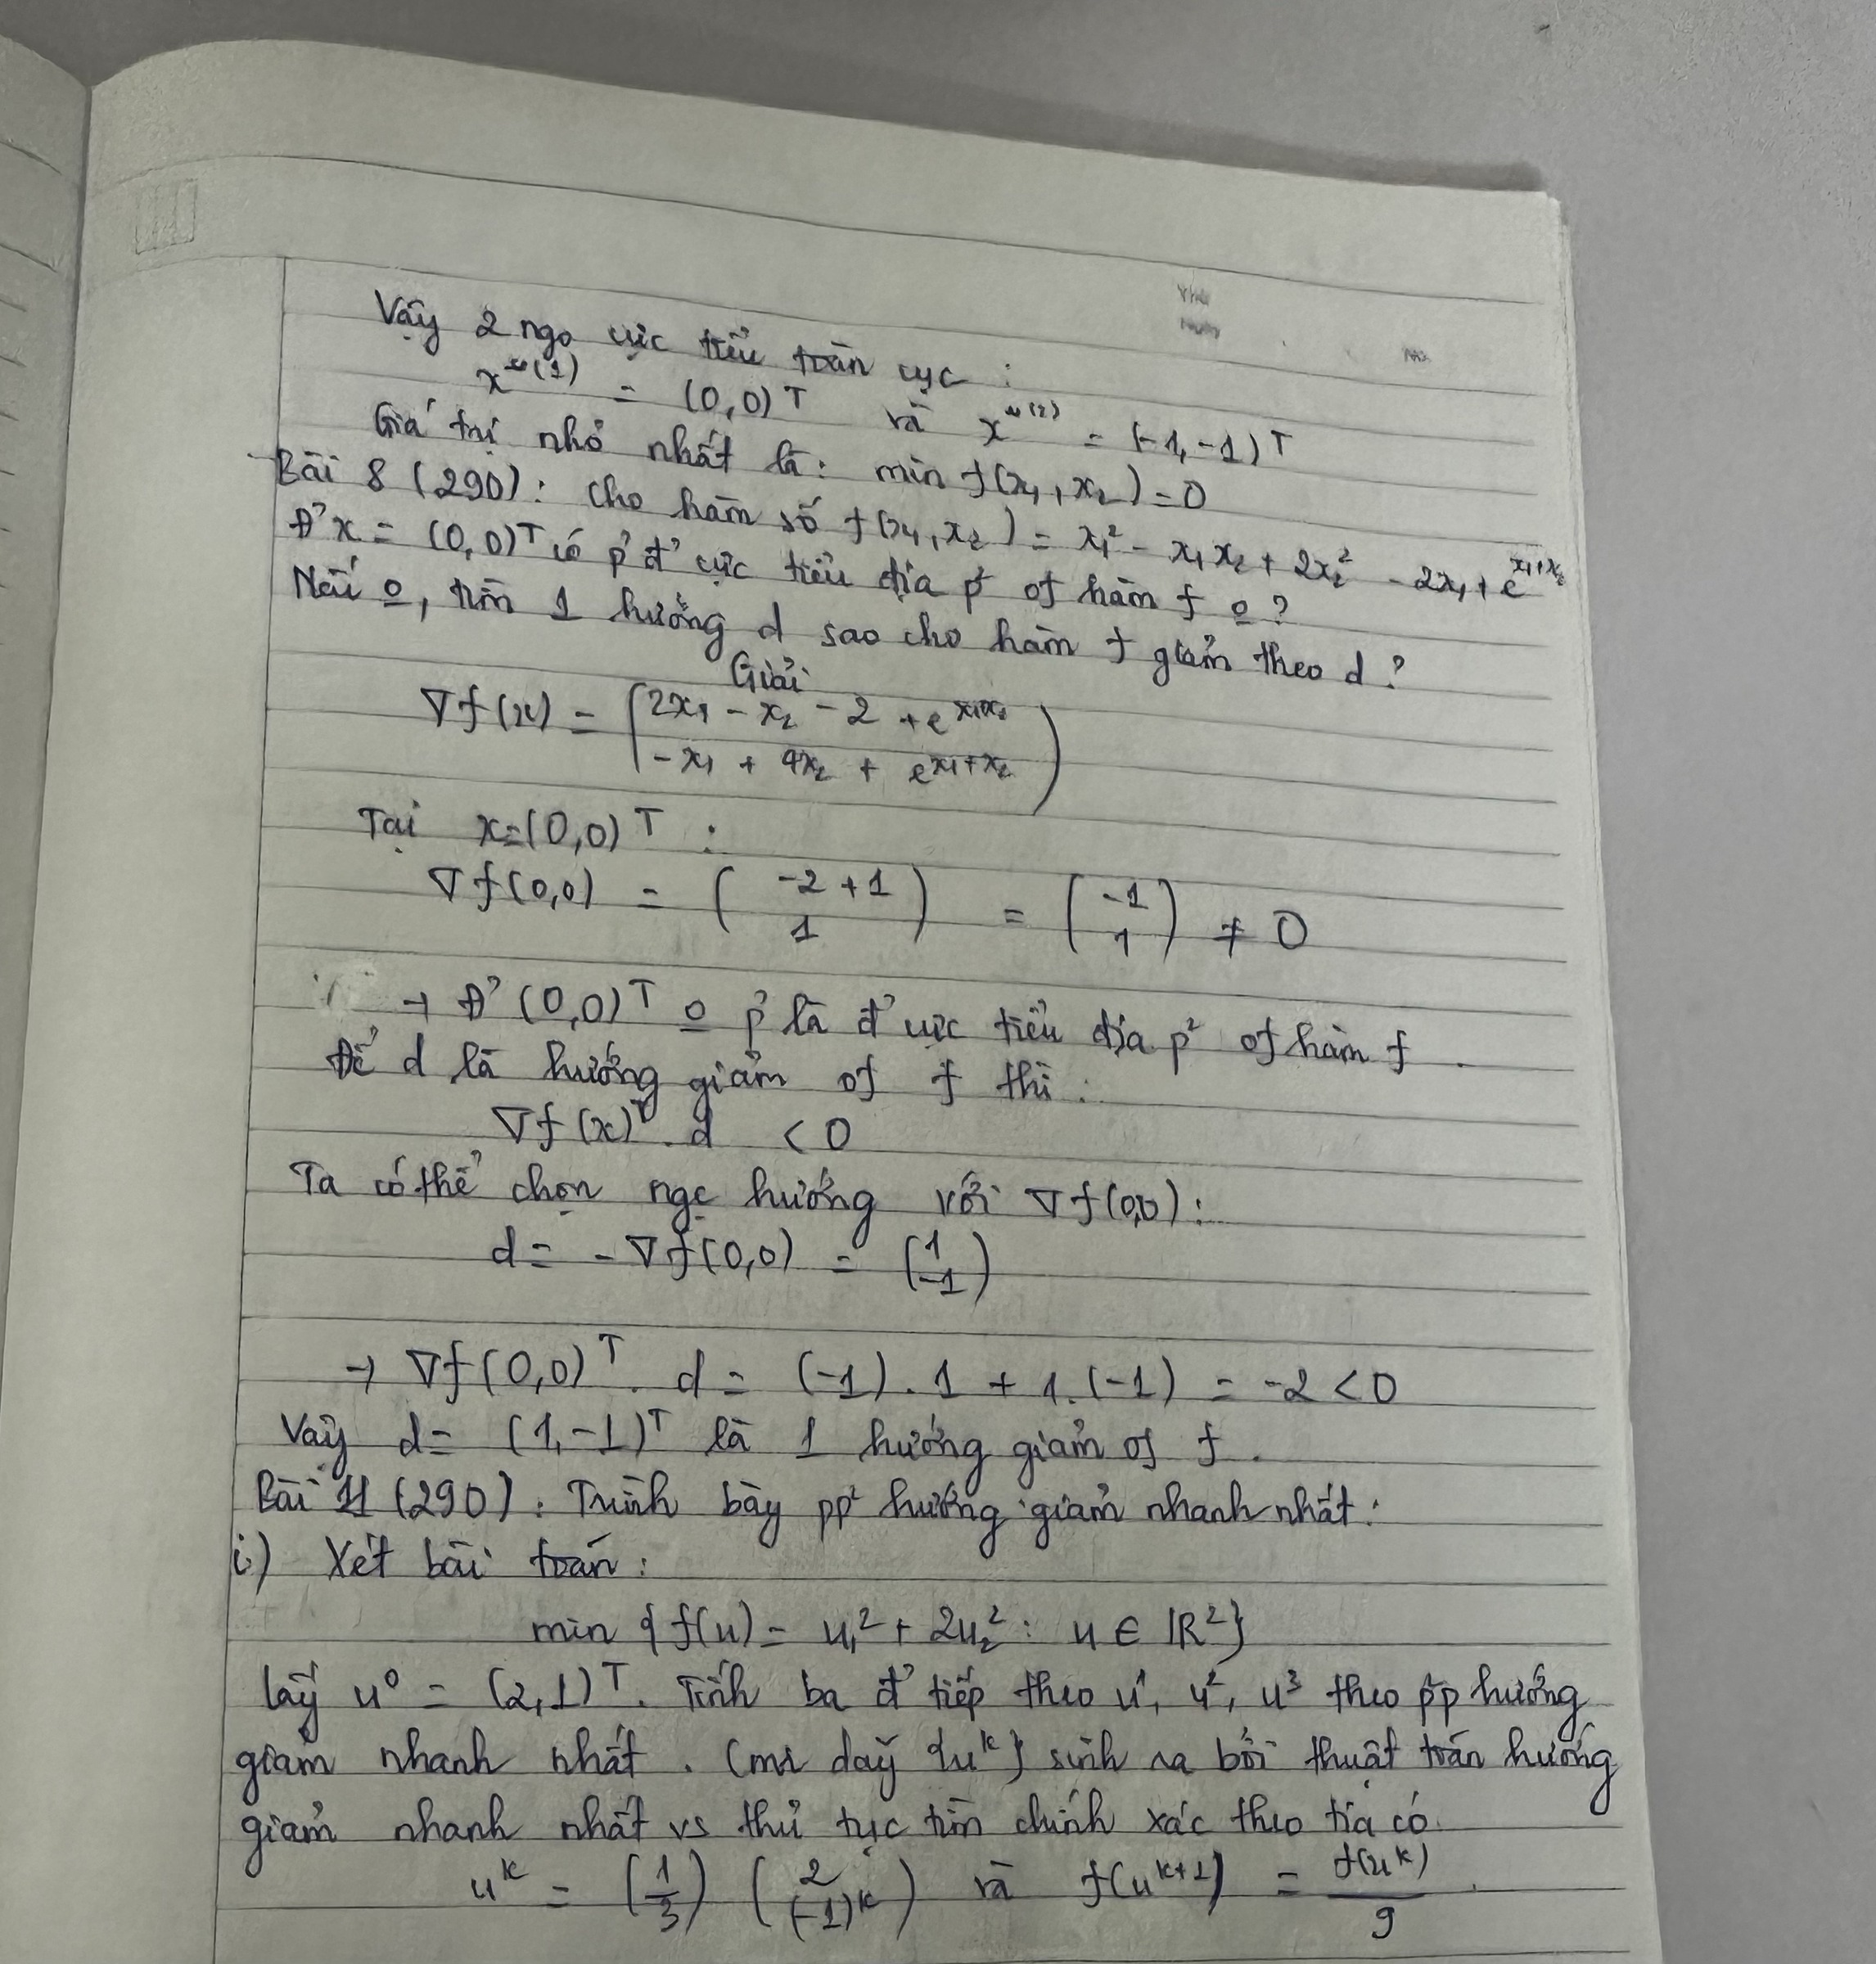
\includegraphics[width=.98\textwidth,height=.82\textheight,keepaspectratio]{bai_lam_them_1_assets/page-078.jpg}\end{center}
\clearpage
\phantomsection\label{src:079}
\noindent\textbf{Ảnh nguồn 079}\par\medskip
\begin{center}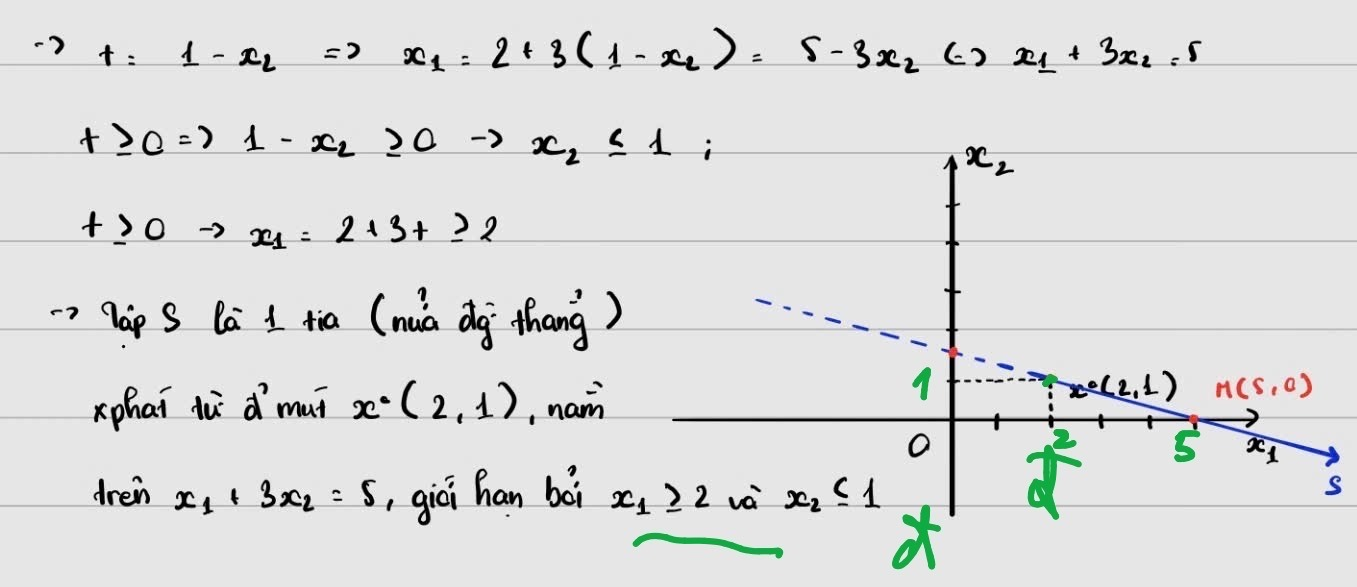
\includegraphics[width=.98\textwidth,height=.82\textheight,keepaspectratio]{bai_lam_them_1_assets/page-079.jpg}\end{center}
\clearpage
\phantomsection\label{src:080}
\noindent\textbf{Ảnh nguồn 080}\par\medskip
\begin{center}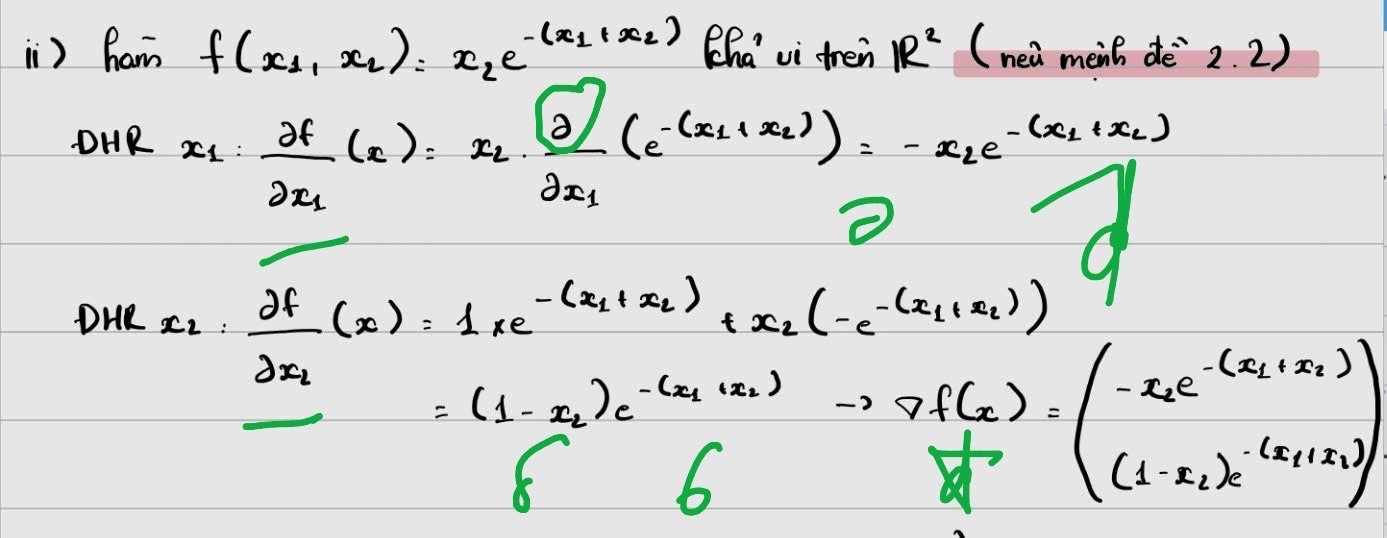
\includegraphics[width=.98\textwidth,height=.82\textheight,keepaspectratio]{bai_lam_them_1_assets/page-080.jpg}\end{center}
\clearpage
\phantomsection\label{src:081}
\noindent\textbf{Ảnh nguồn 081}\par\medskip
\begin{center}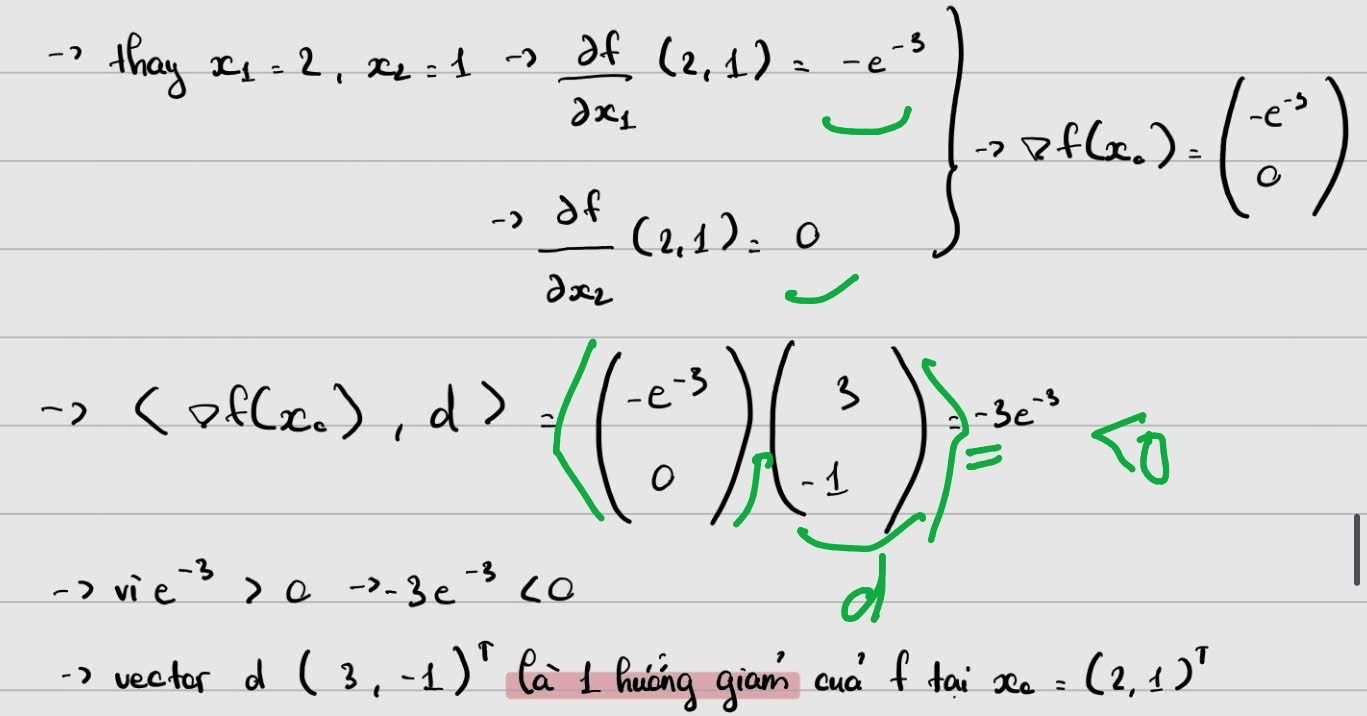
\includegraphics[width=.98\textwidth,height=.82\textheight,keepaspectratio]{bai_lam_them_1_assets/page-081.jpg}\end{center}
\clearpage
\phantomsection\label{src:082}
\noindent\textbf{Ảnh nguồn 082}\par\medskip
\begin{center}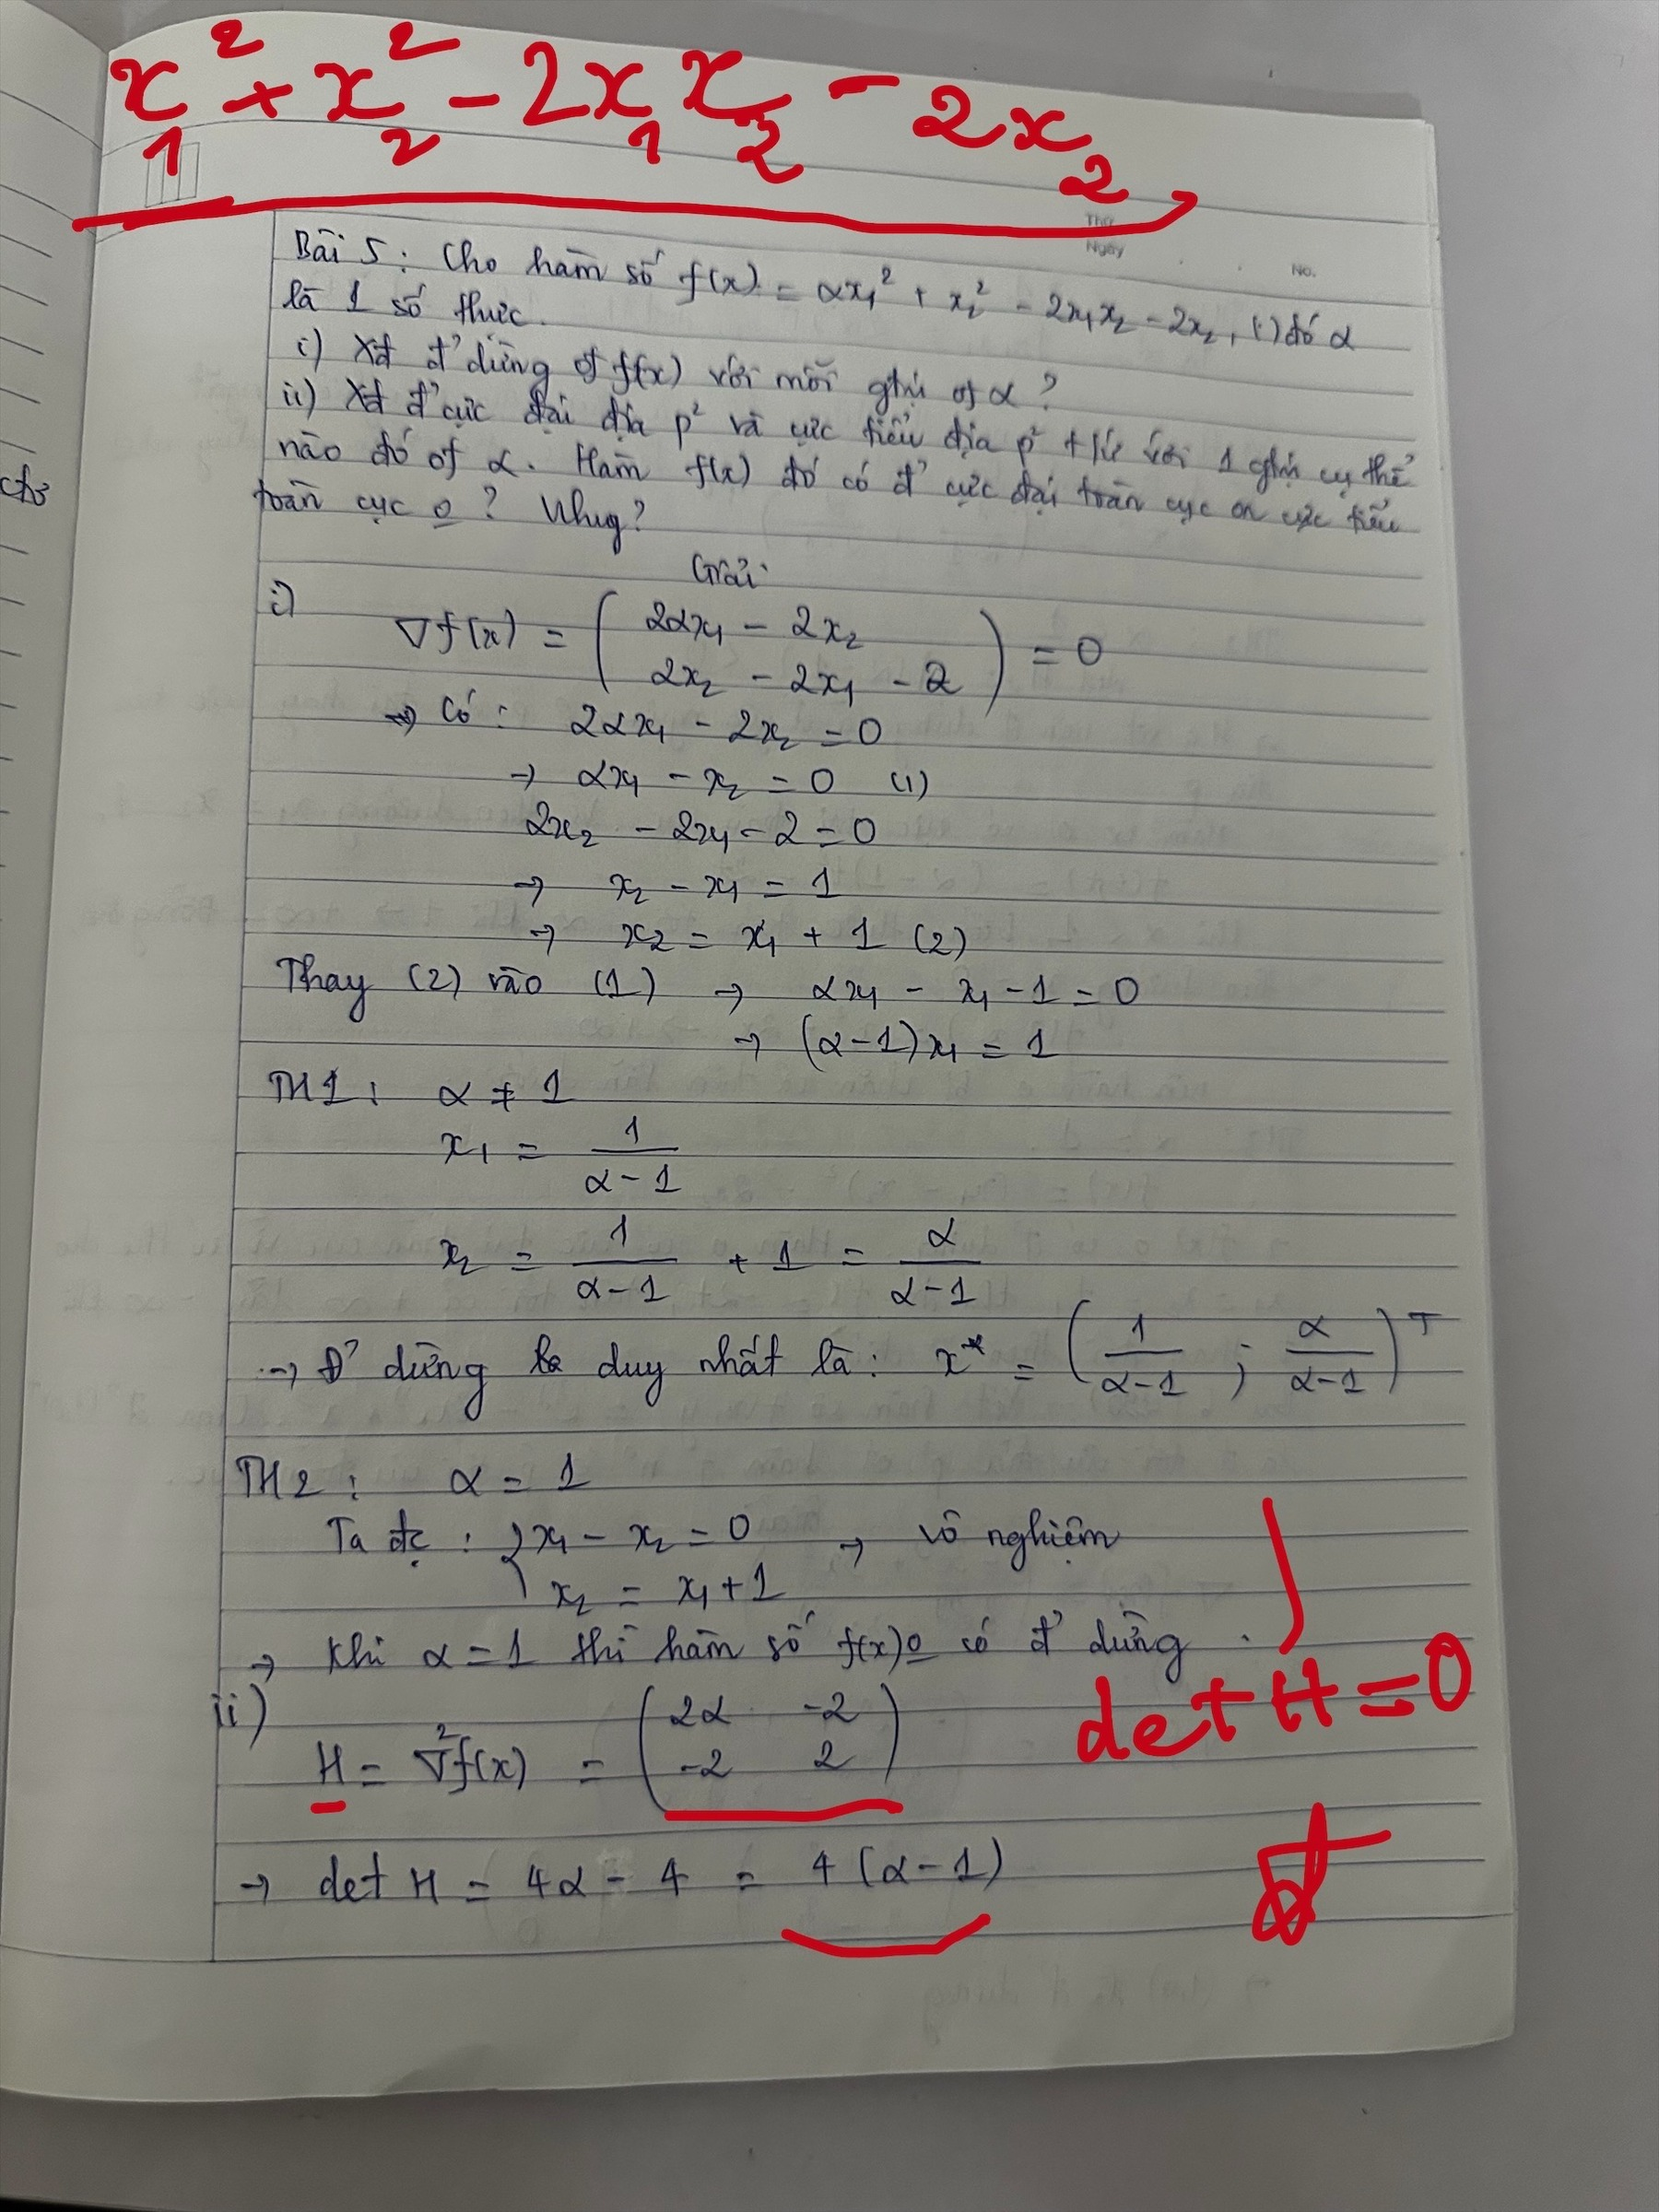
\includegraphics[width=.98\textwidth,height=.82\textheight,keepaspectratio]{bai_lam_them_1_assets/page-082.jpg}\end{center}
\clearpage
\phantomsection\label{src:083}
\noindent\textbf{Ảnh nguồn 083}\par\medskip
\begin{center}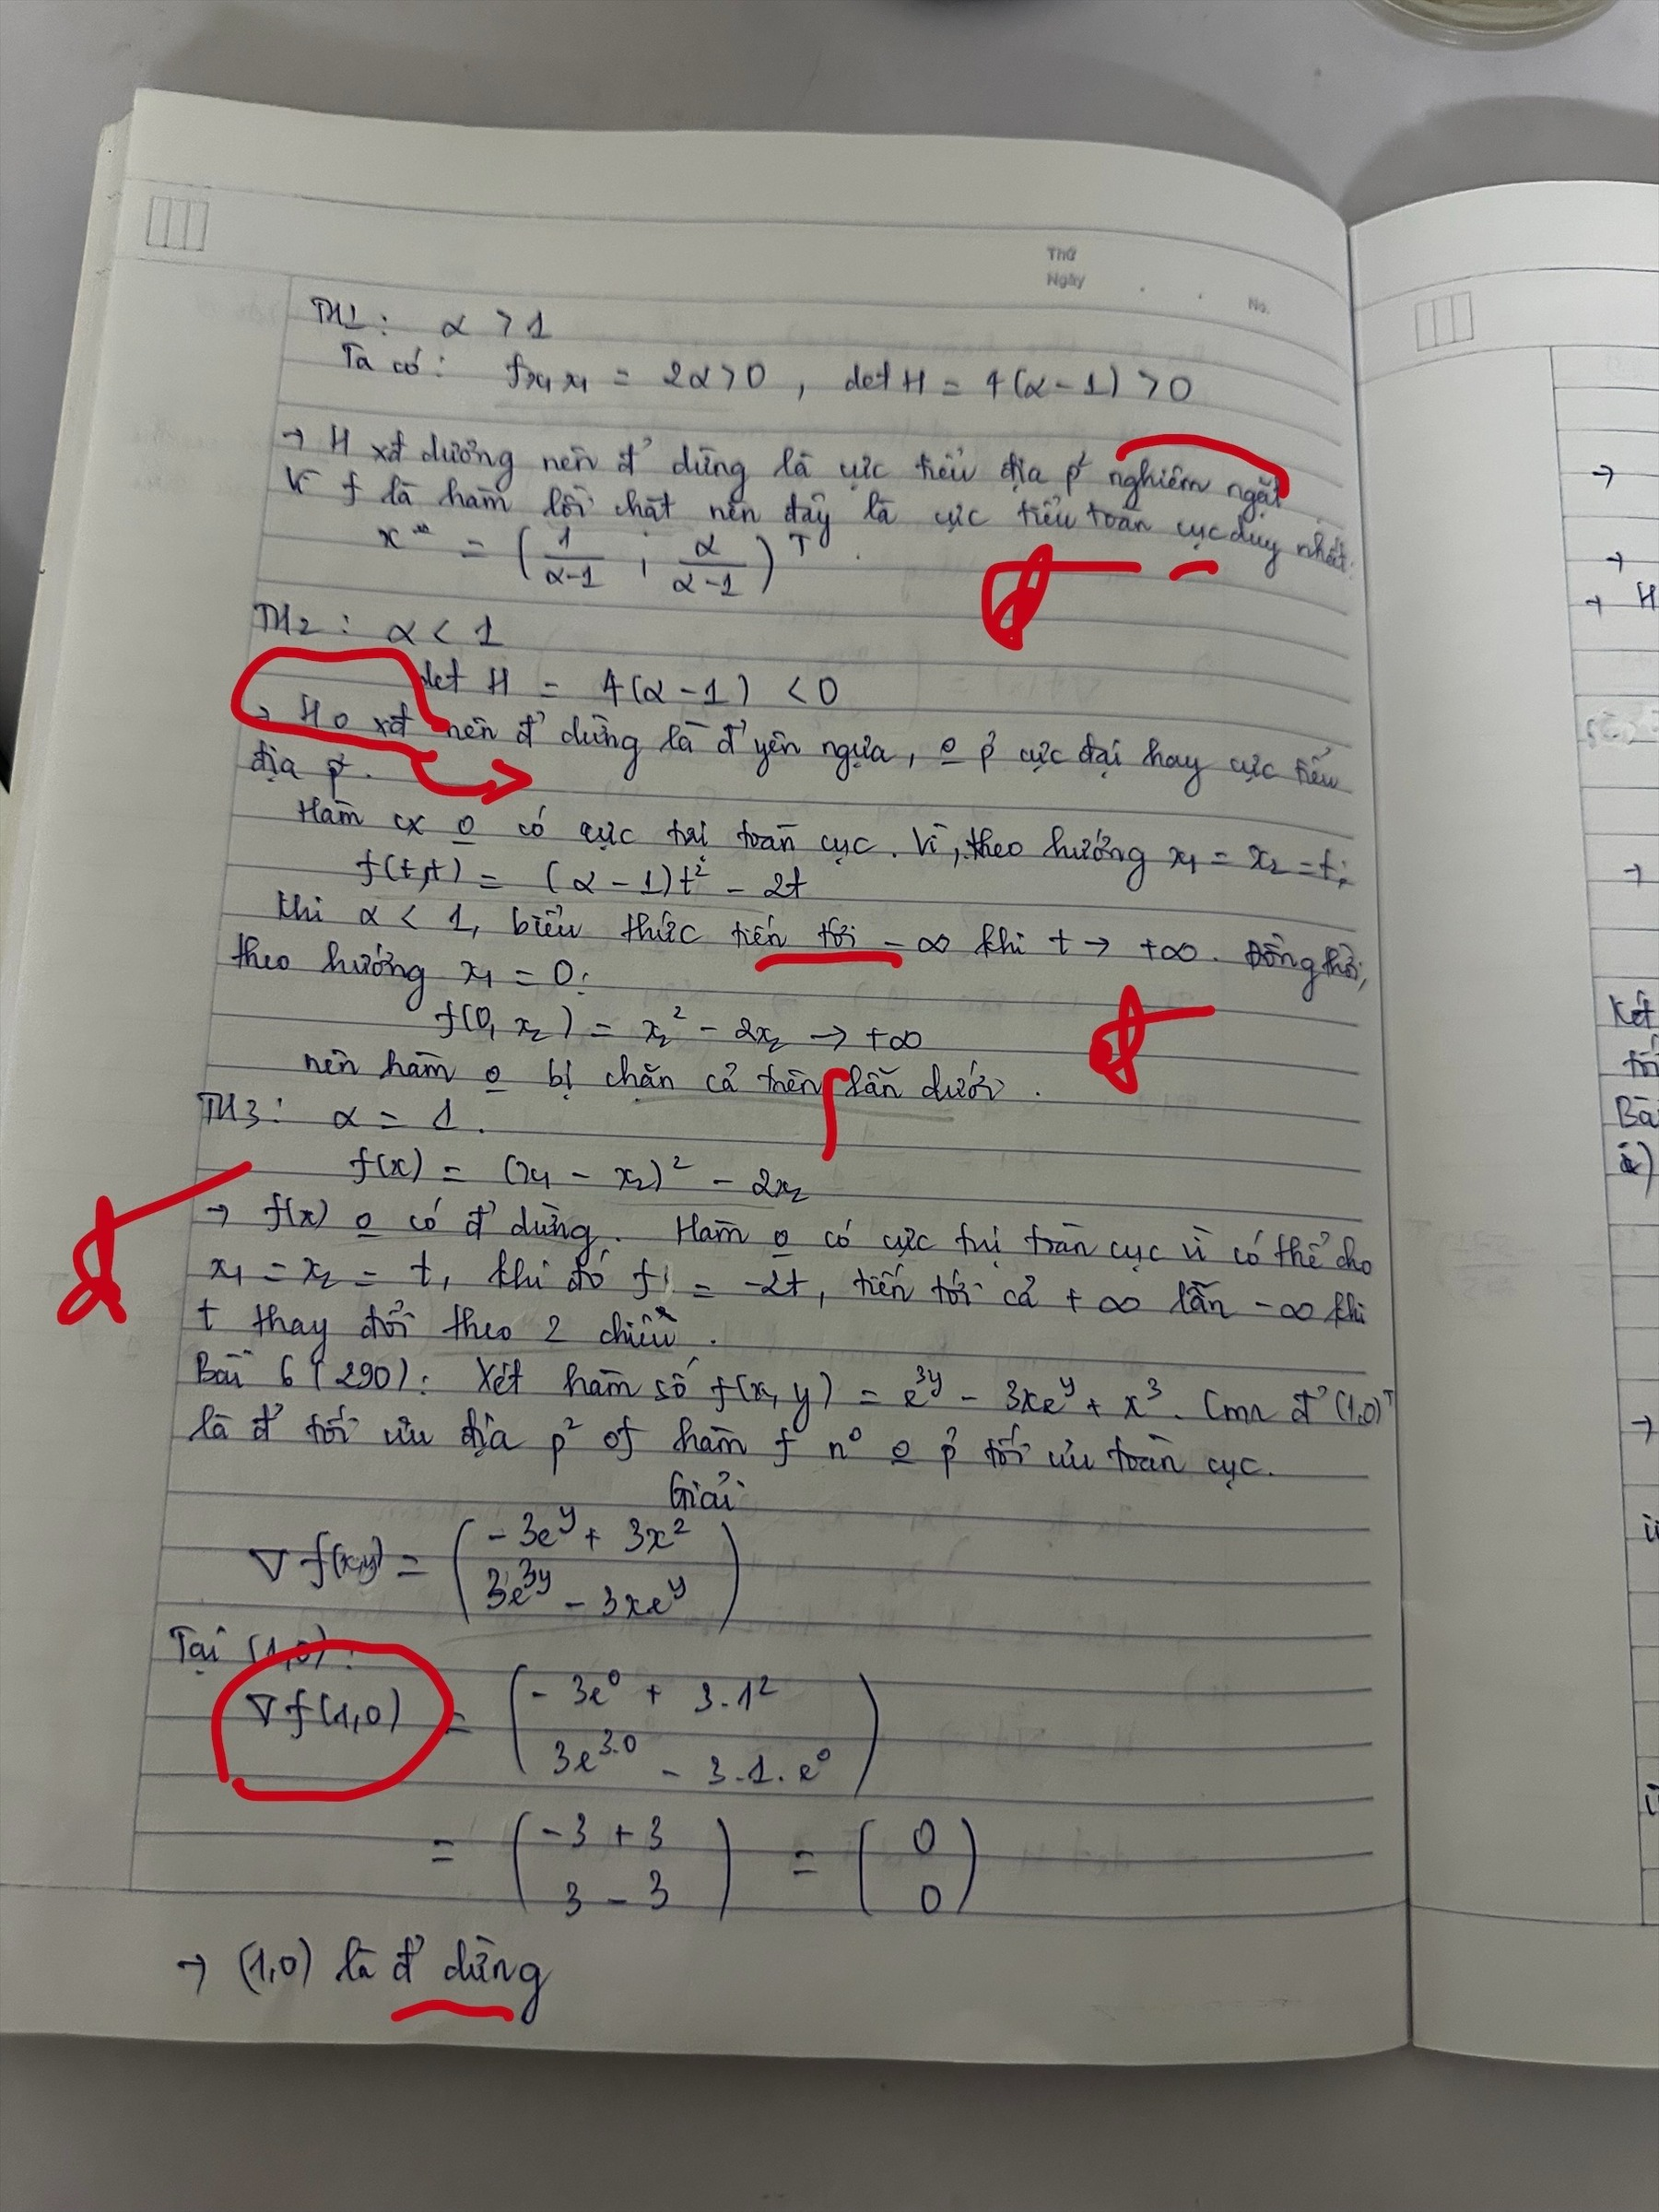
\includegraphics[width=.98\textwidth,height=.82\textheight,keepaspectratio]{bai_lam_them_1_assets/page-083.jpg}\end{center}
\clearpage
\phantomsection\label{src:084}
\noindent\textbf{Ảnh nguồn 084}\par\medskip
\begin{center}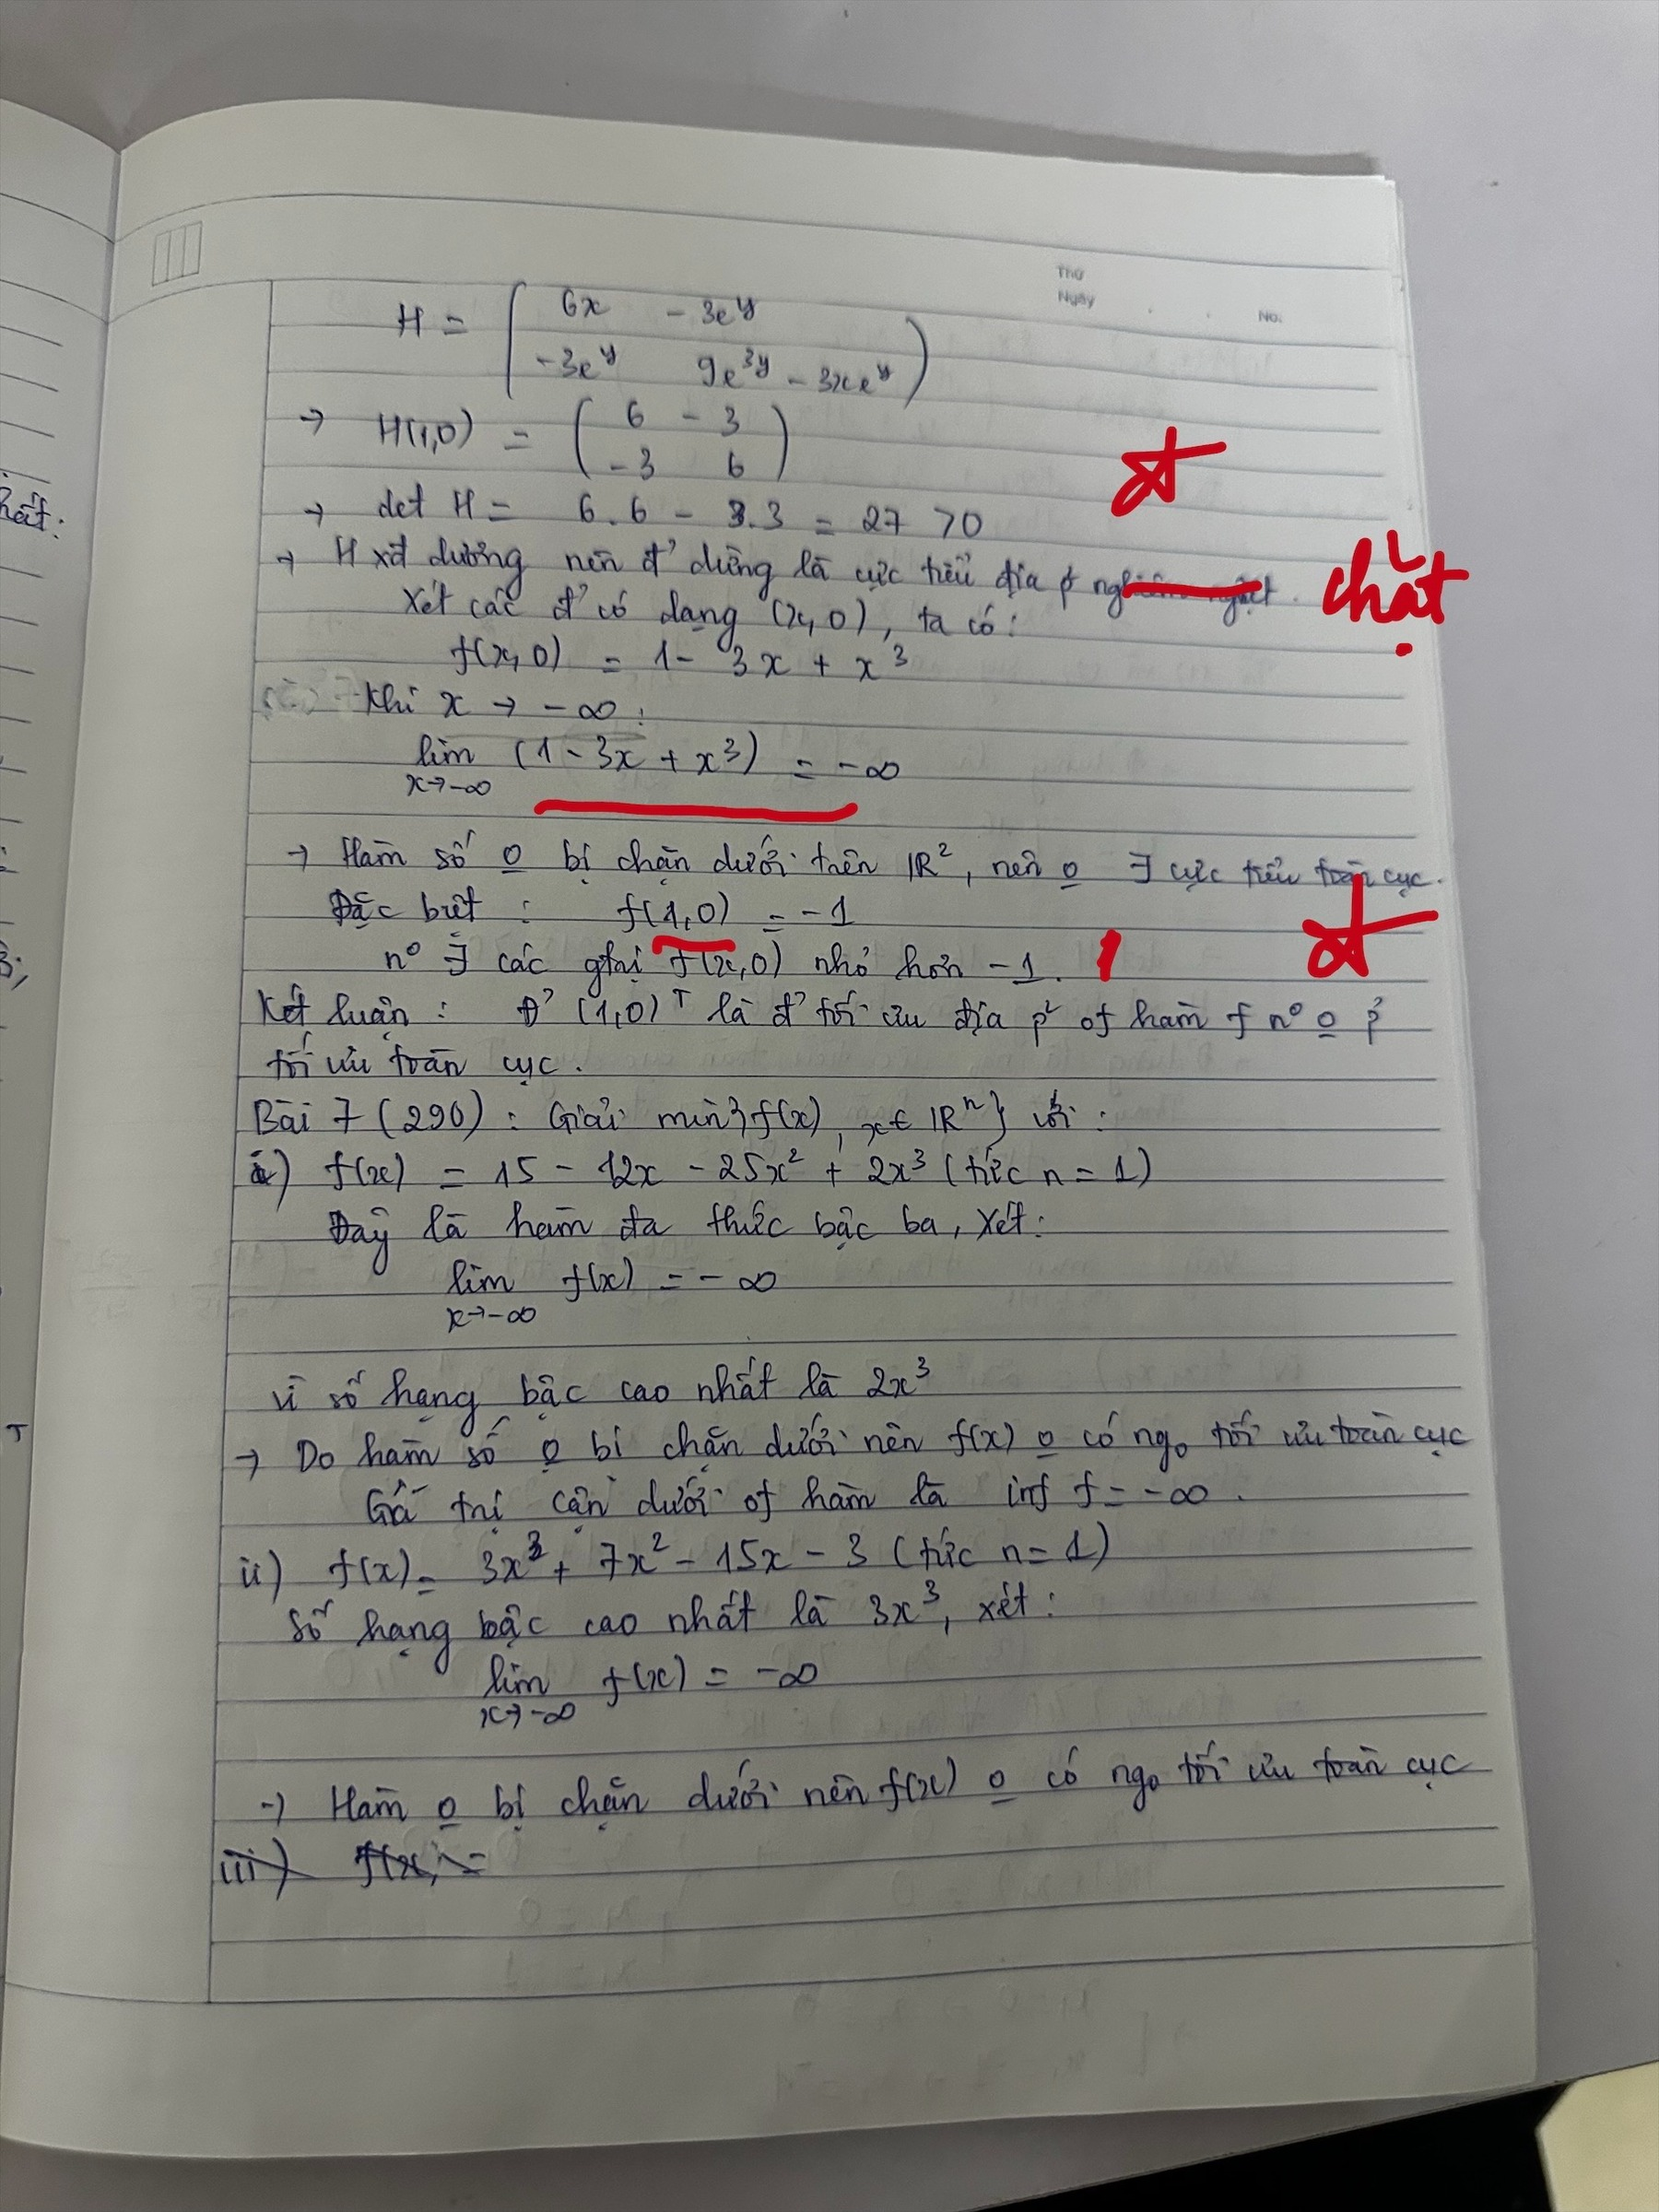
\includegraphics[width=.98\textwidth,height=.82\textheight,keepaspectratio]{bai_lam_them_1_assets/page-084.jpg}\end{center}
\clearpage
\phantomsection\label{src:085}
\noindent\textbf{Ảnh nguồn 085}\par\medskip
\begin{center}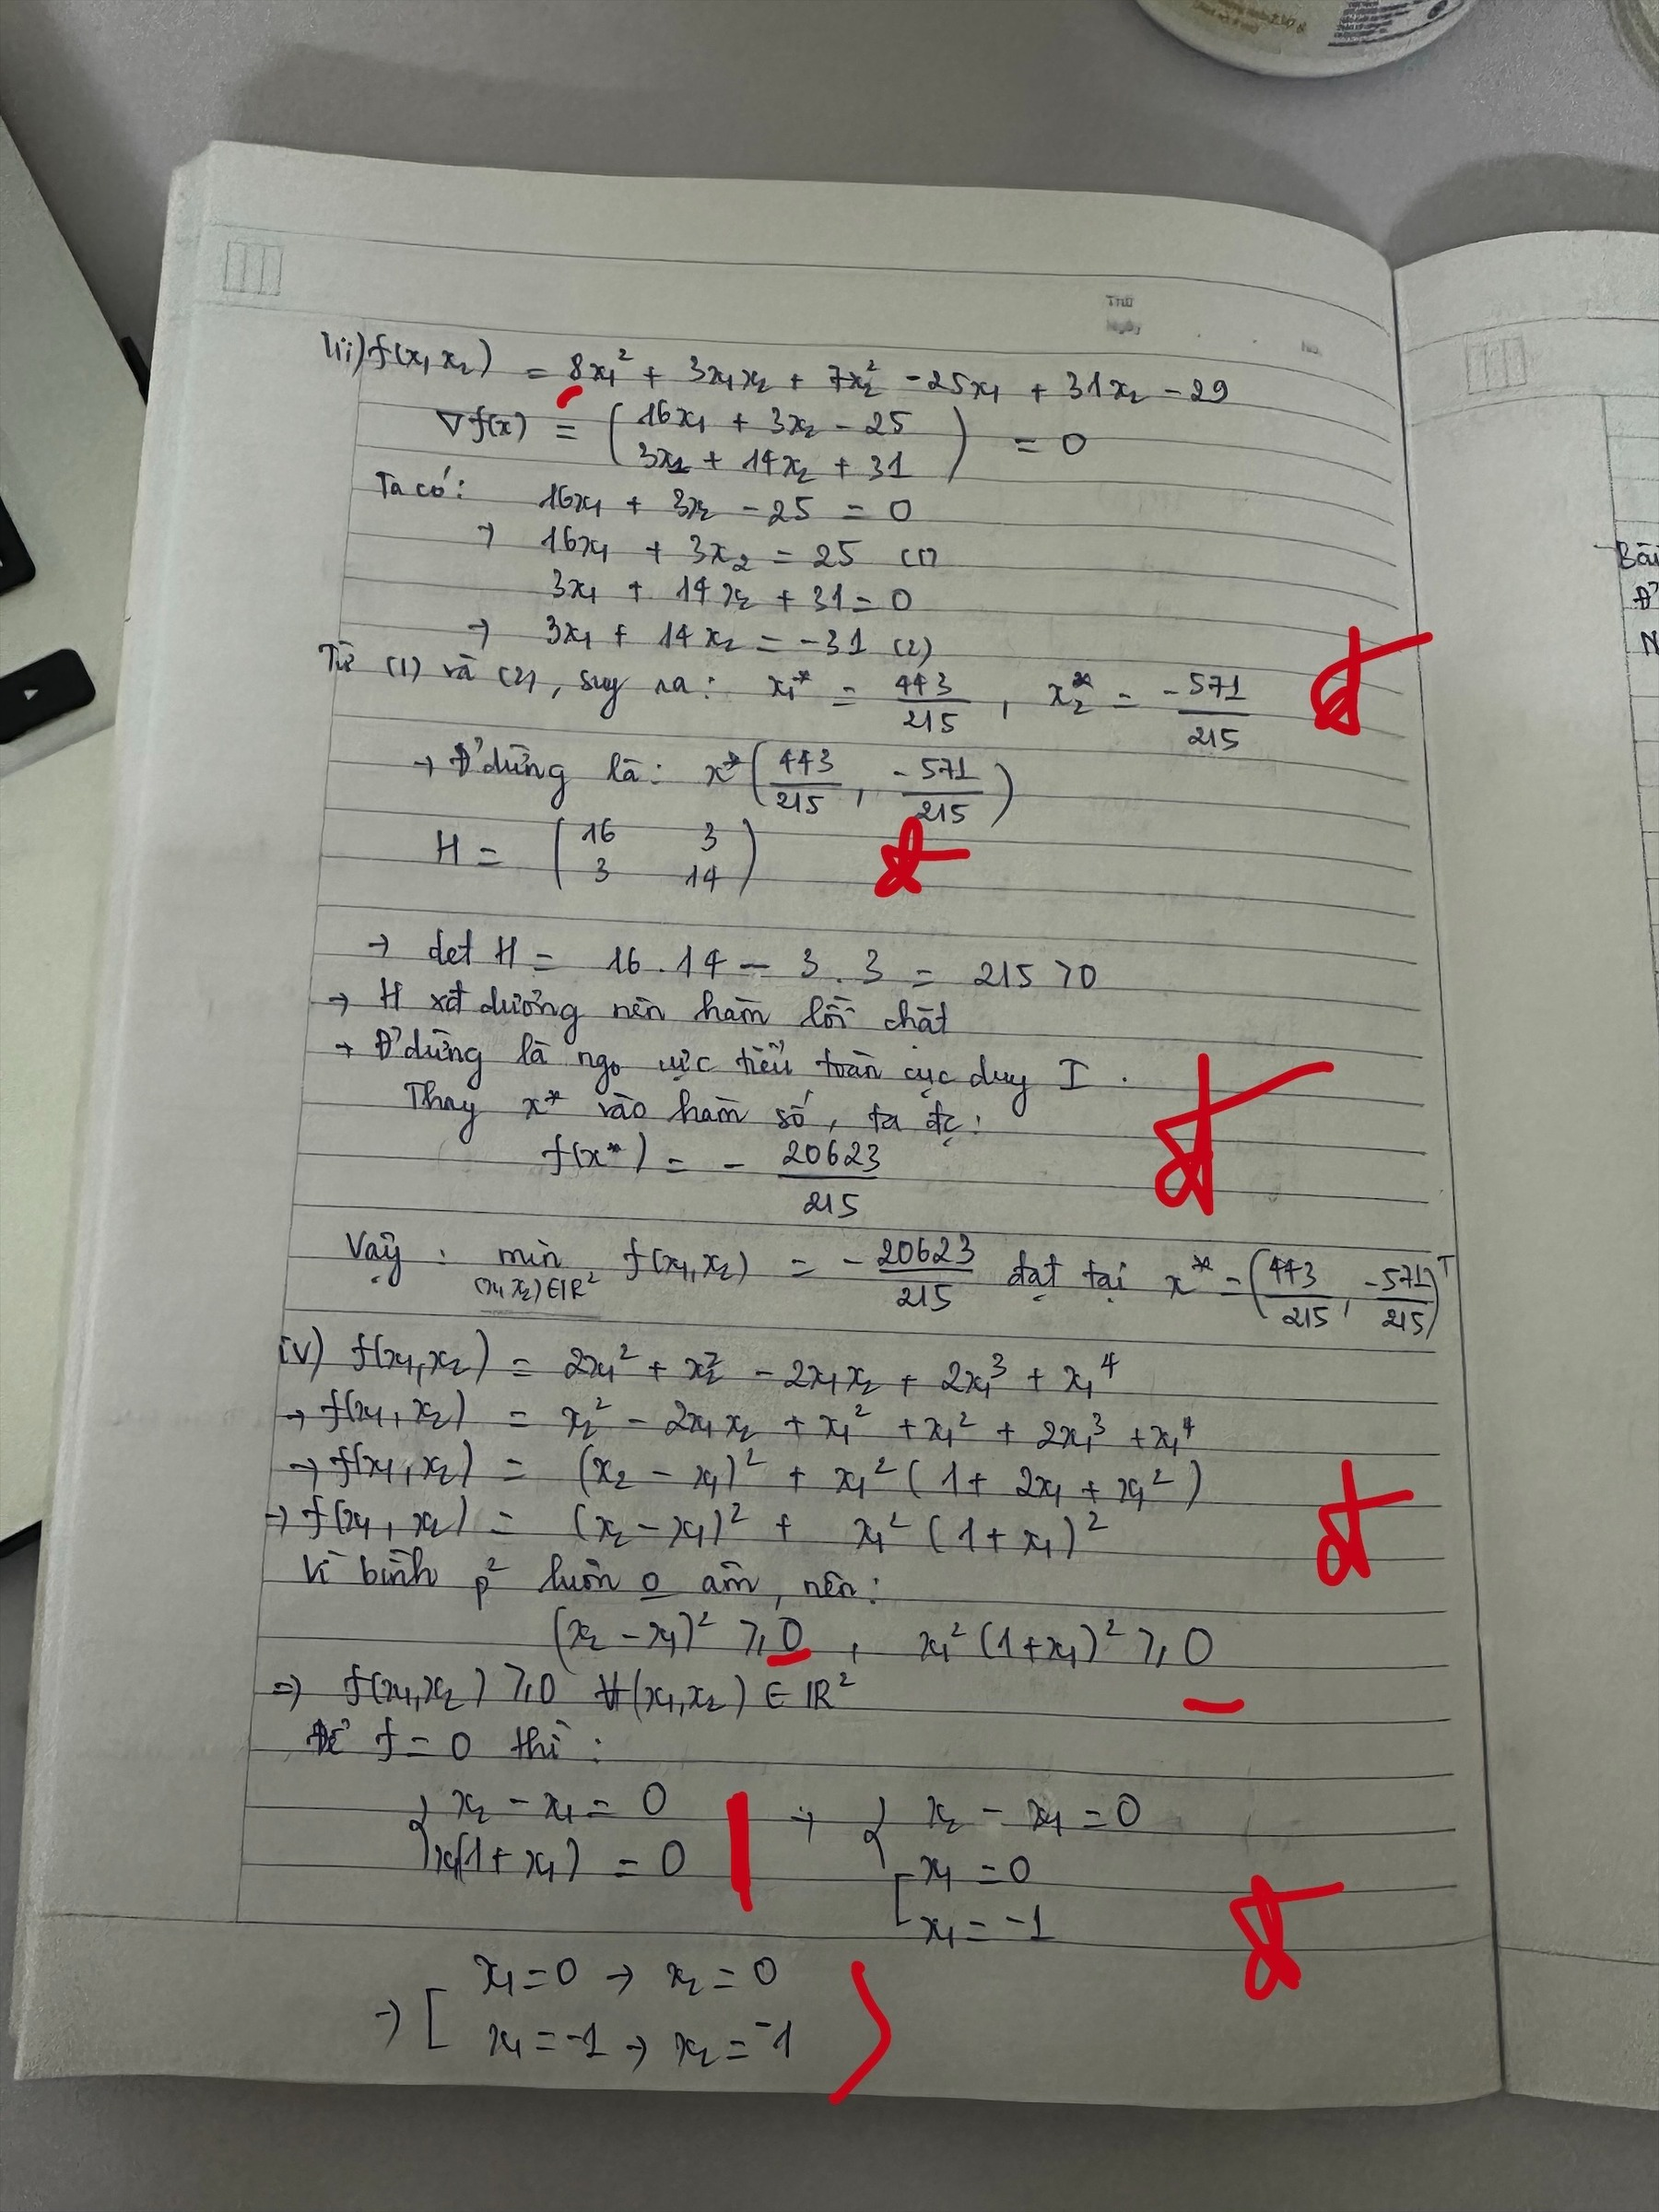
\includegraphics[width=.98\textwidth,height=.82\textheight,keepaspectratio]{bai_lam_them_1_assets/page-085.jpg}\end{center}
\clearpage
\phantomsection\label{src:086}
\noindent\textbf{Ảnh nguồn 086}\par\medskip
\begin{center}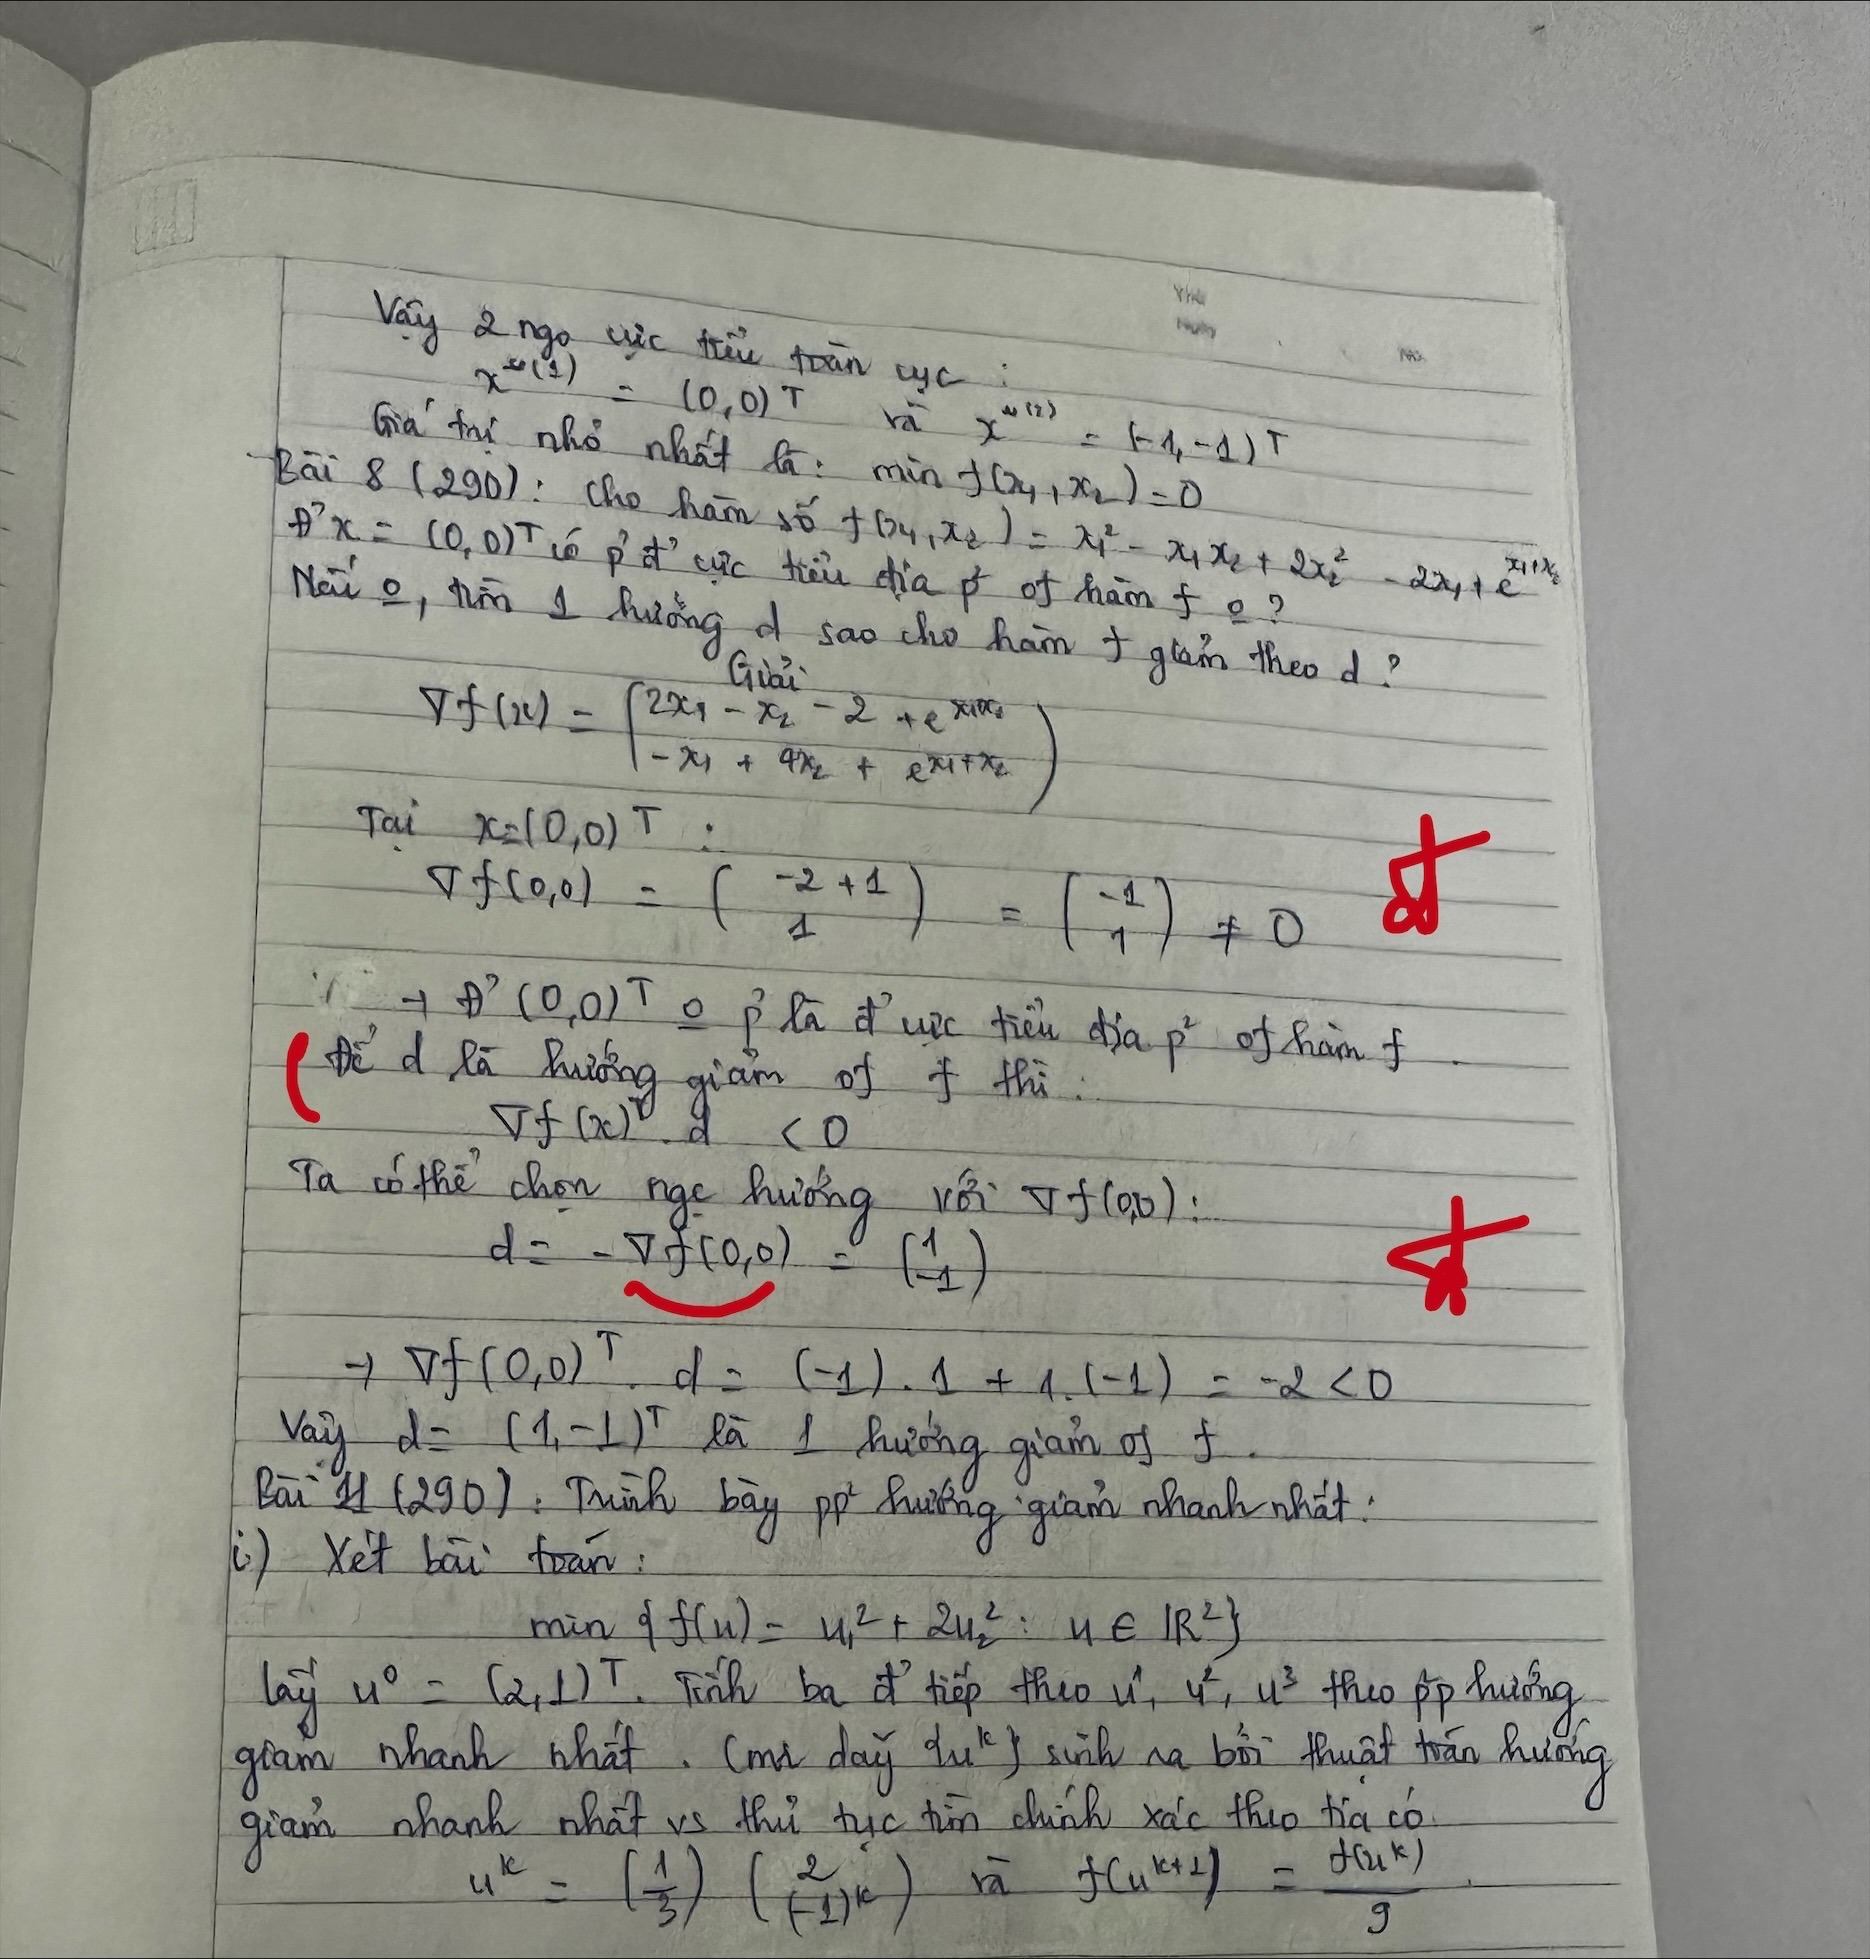
\includegraphics[width=.98\textwidth,height=.82\textheight,keepaspectratio]{bai_lam_them_1_assets/page-086.jpg}\end{center}
\clearpage
\phantomsection\label{src:087}
\noindent\textbf{Ảnh nguồn 087}\par\medskip
\begin{center}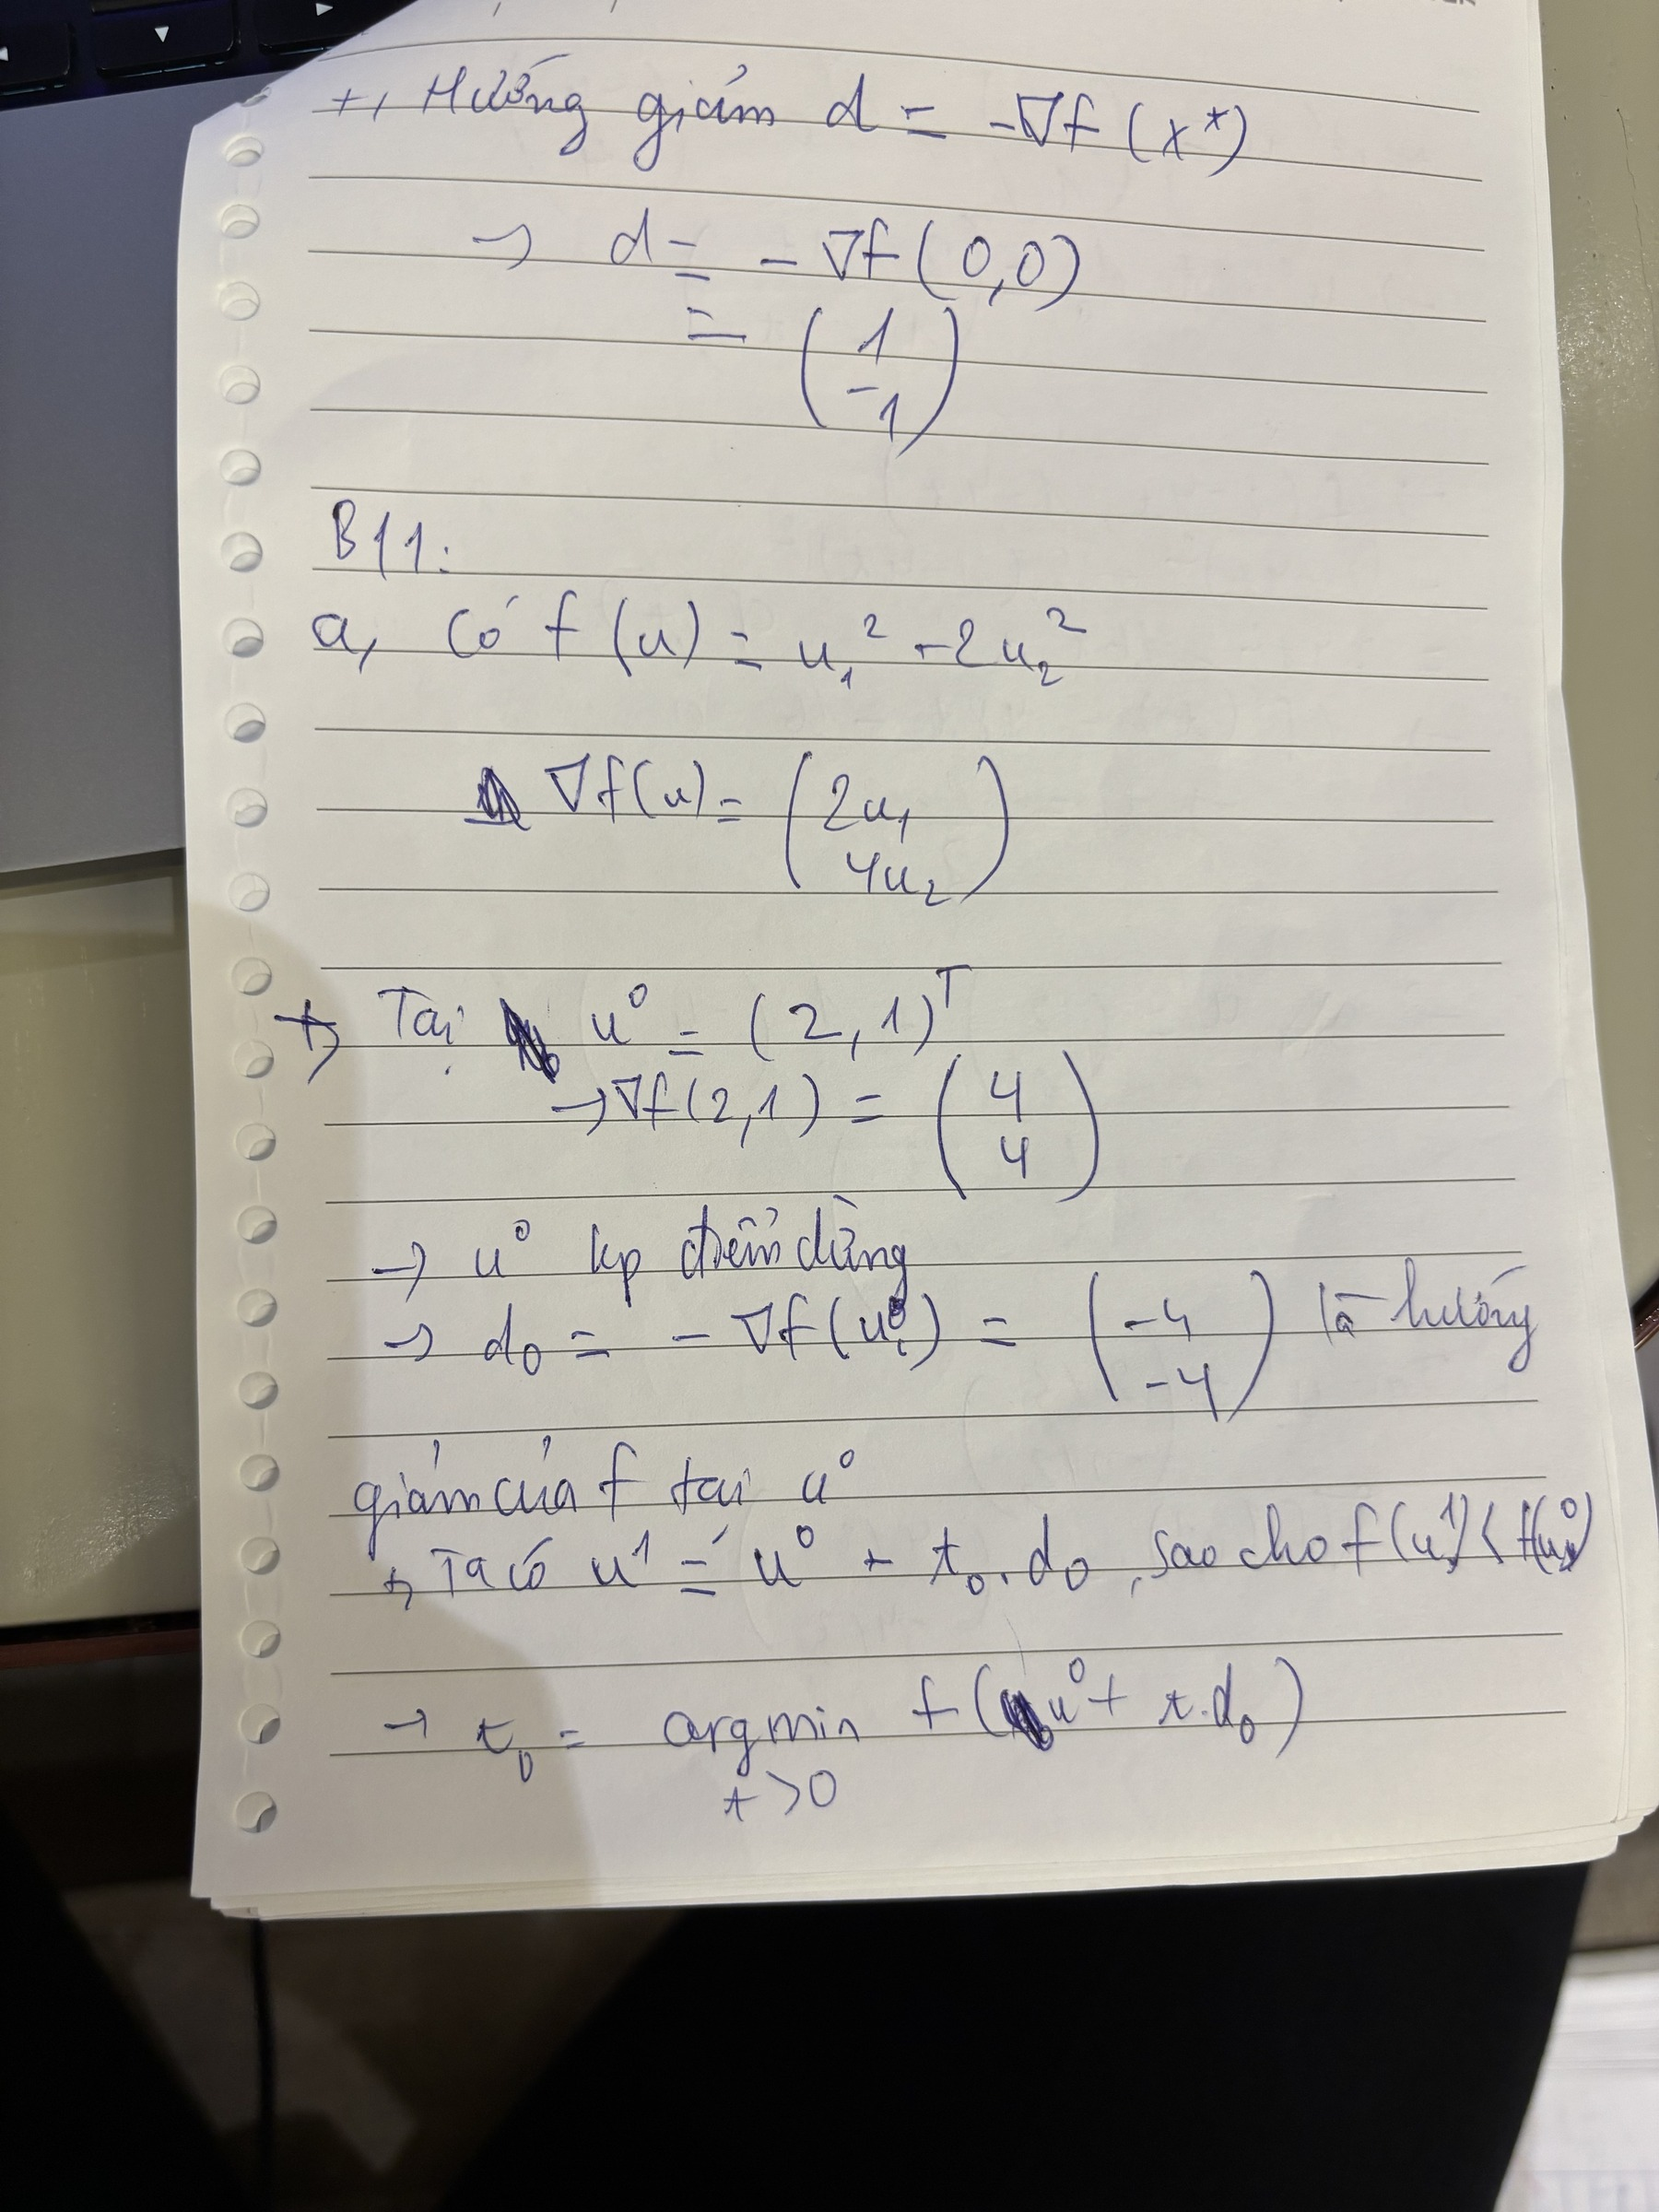
\includegraphics[width=.98\textwidth,height=.82\textheight,keepaspectratio]{bai_lam_them_1_assets/page-087.jpg}\end{center}
\clearpage
\phantomsection\label{src:088}
\noindent\textbf{Ảnh nguồn 088}\par\medskip
\begin{center}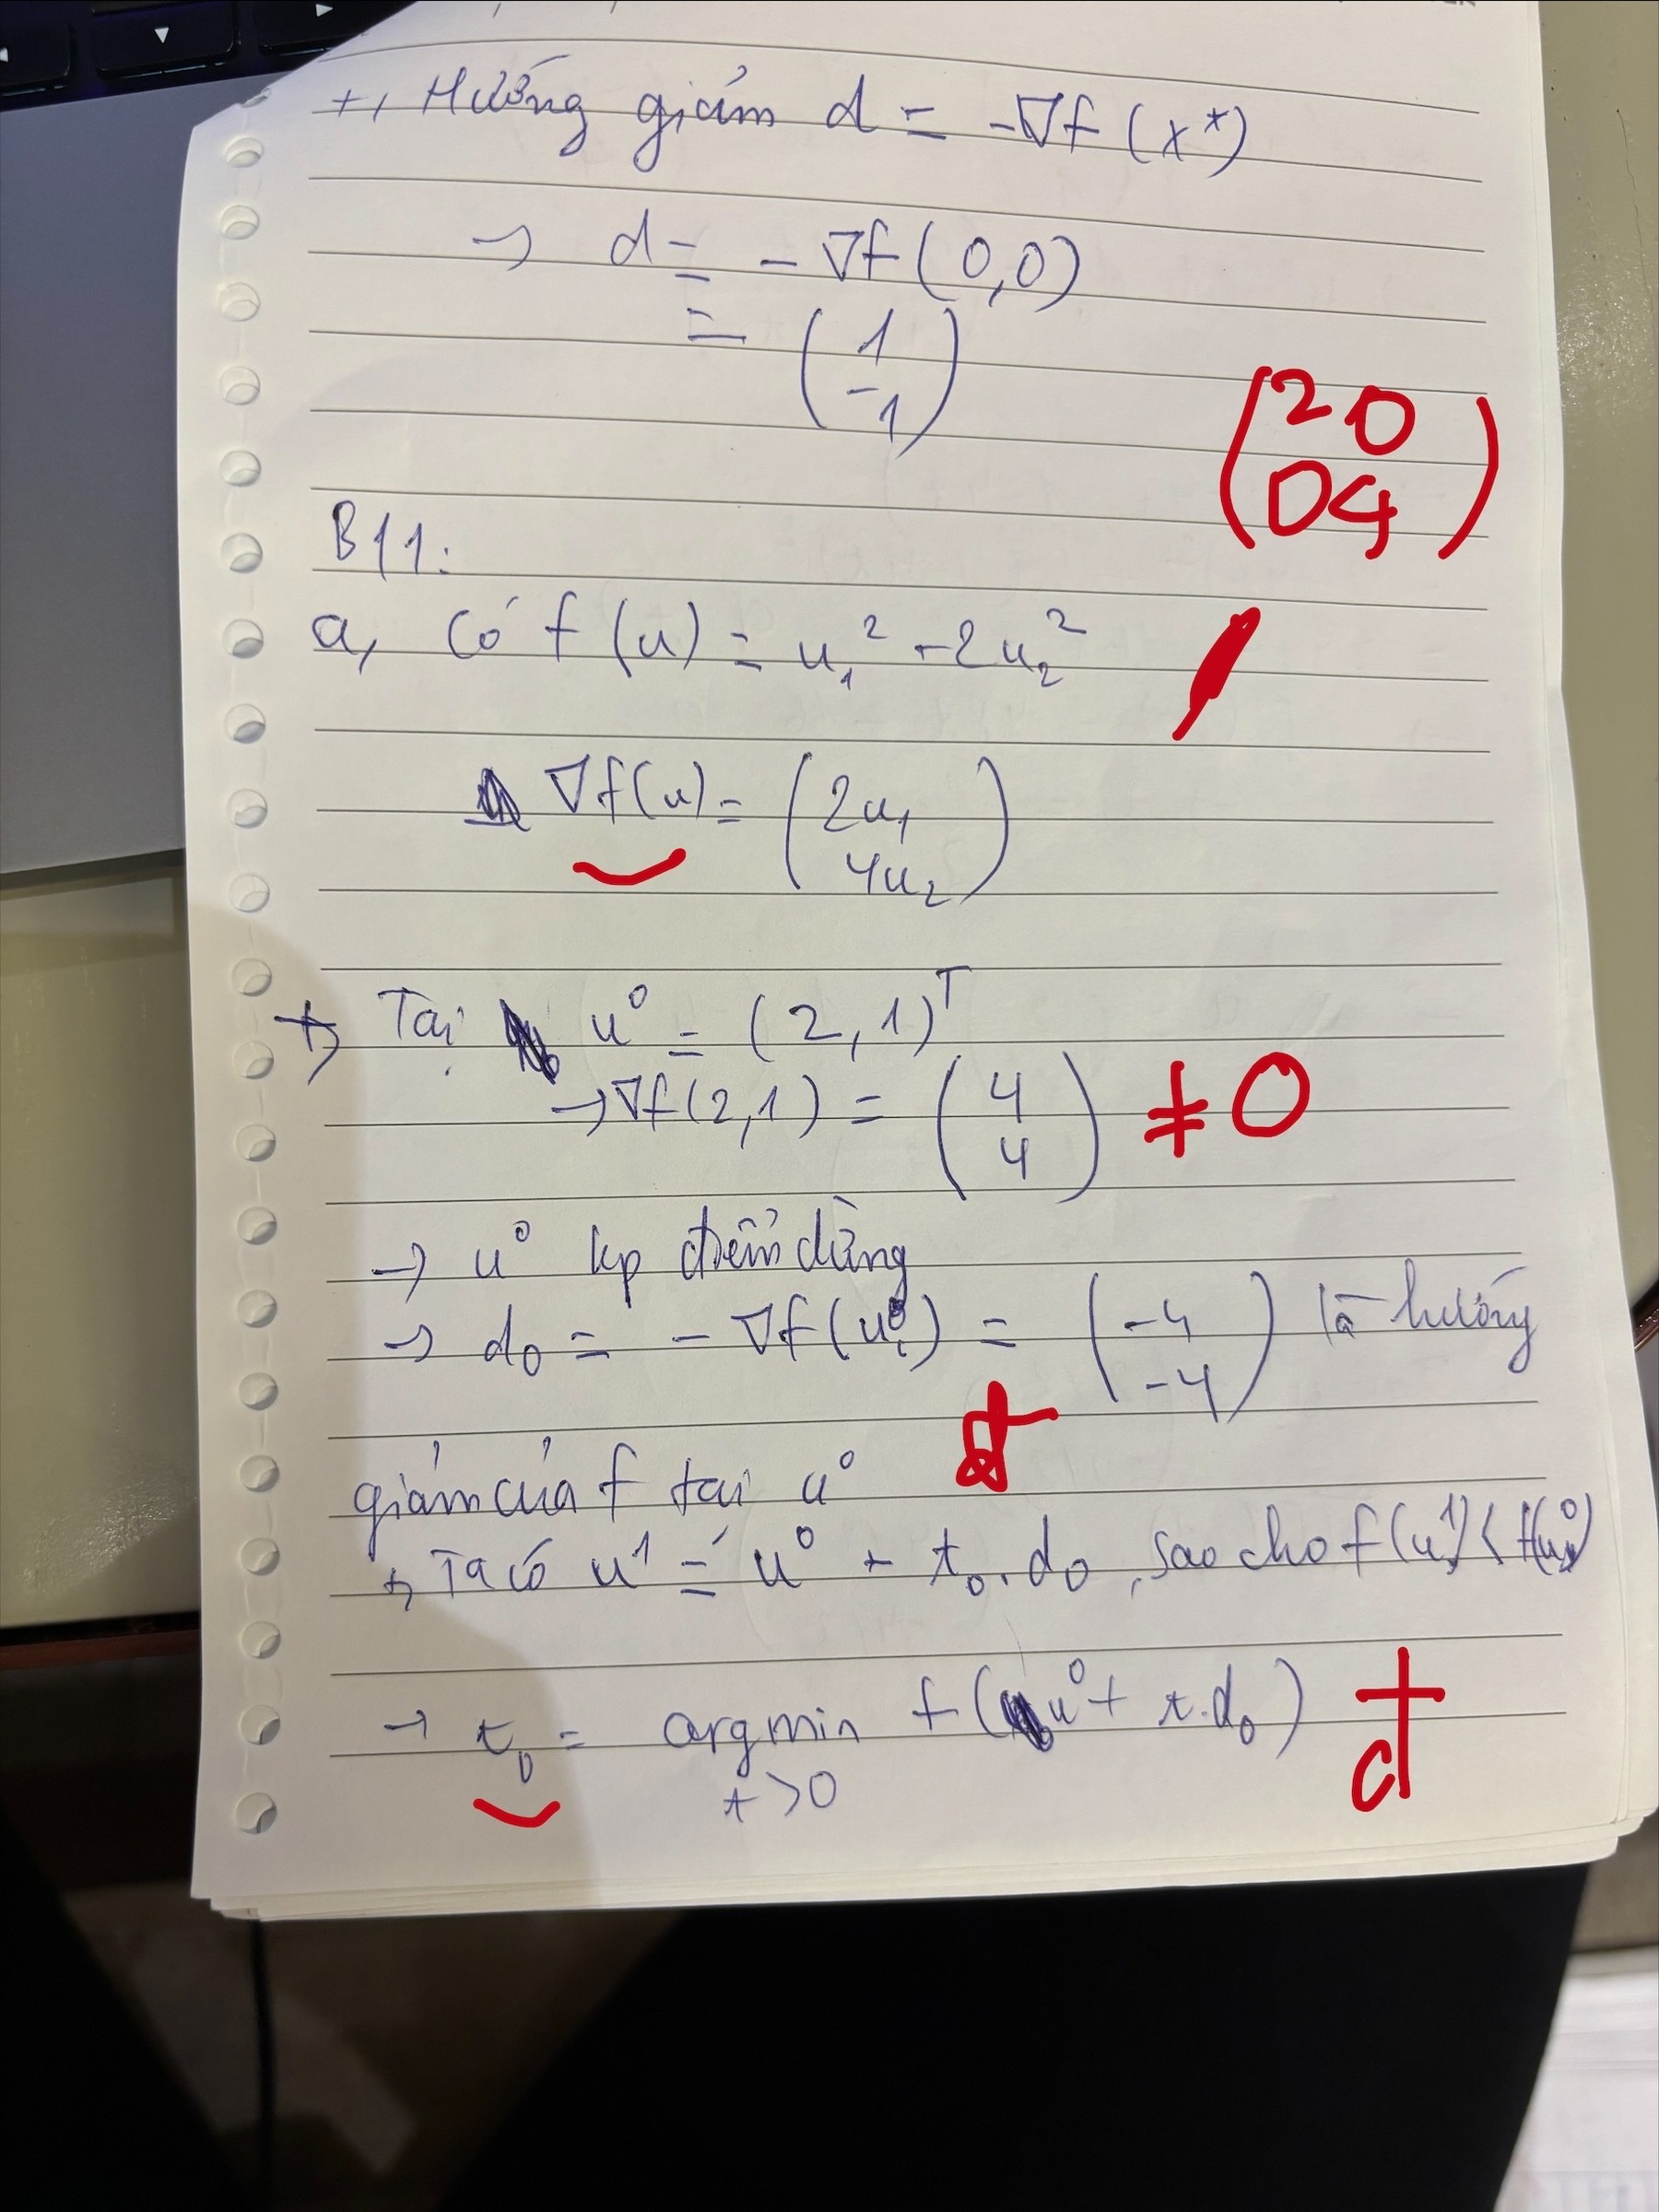
\includegraphics[width=.98\textwidth,height=.82\textheight,keepaspectratio]{bai_lam_them_1_assets/page-088.jpg}\end{center}
\clearpage
\phantomsection\label{src:089}
\noindent\textbf{Ảnh nguồn 089}\par\medskip
\begin{center}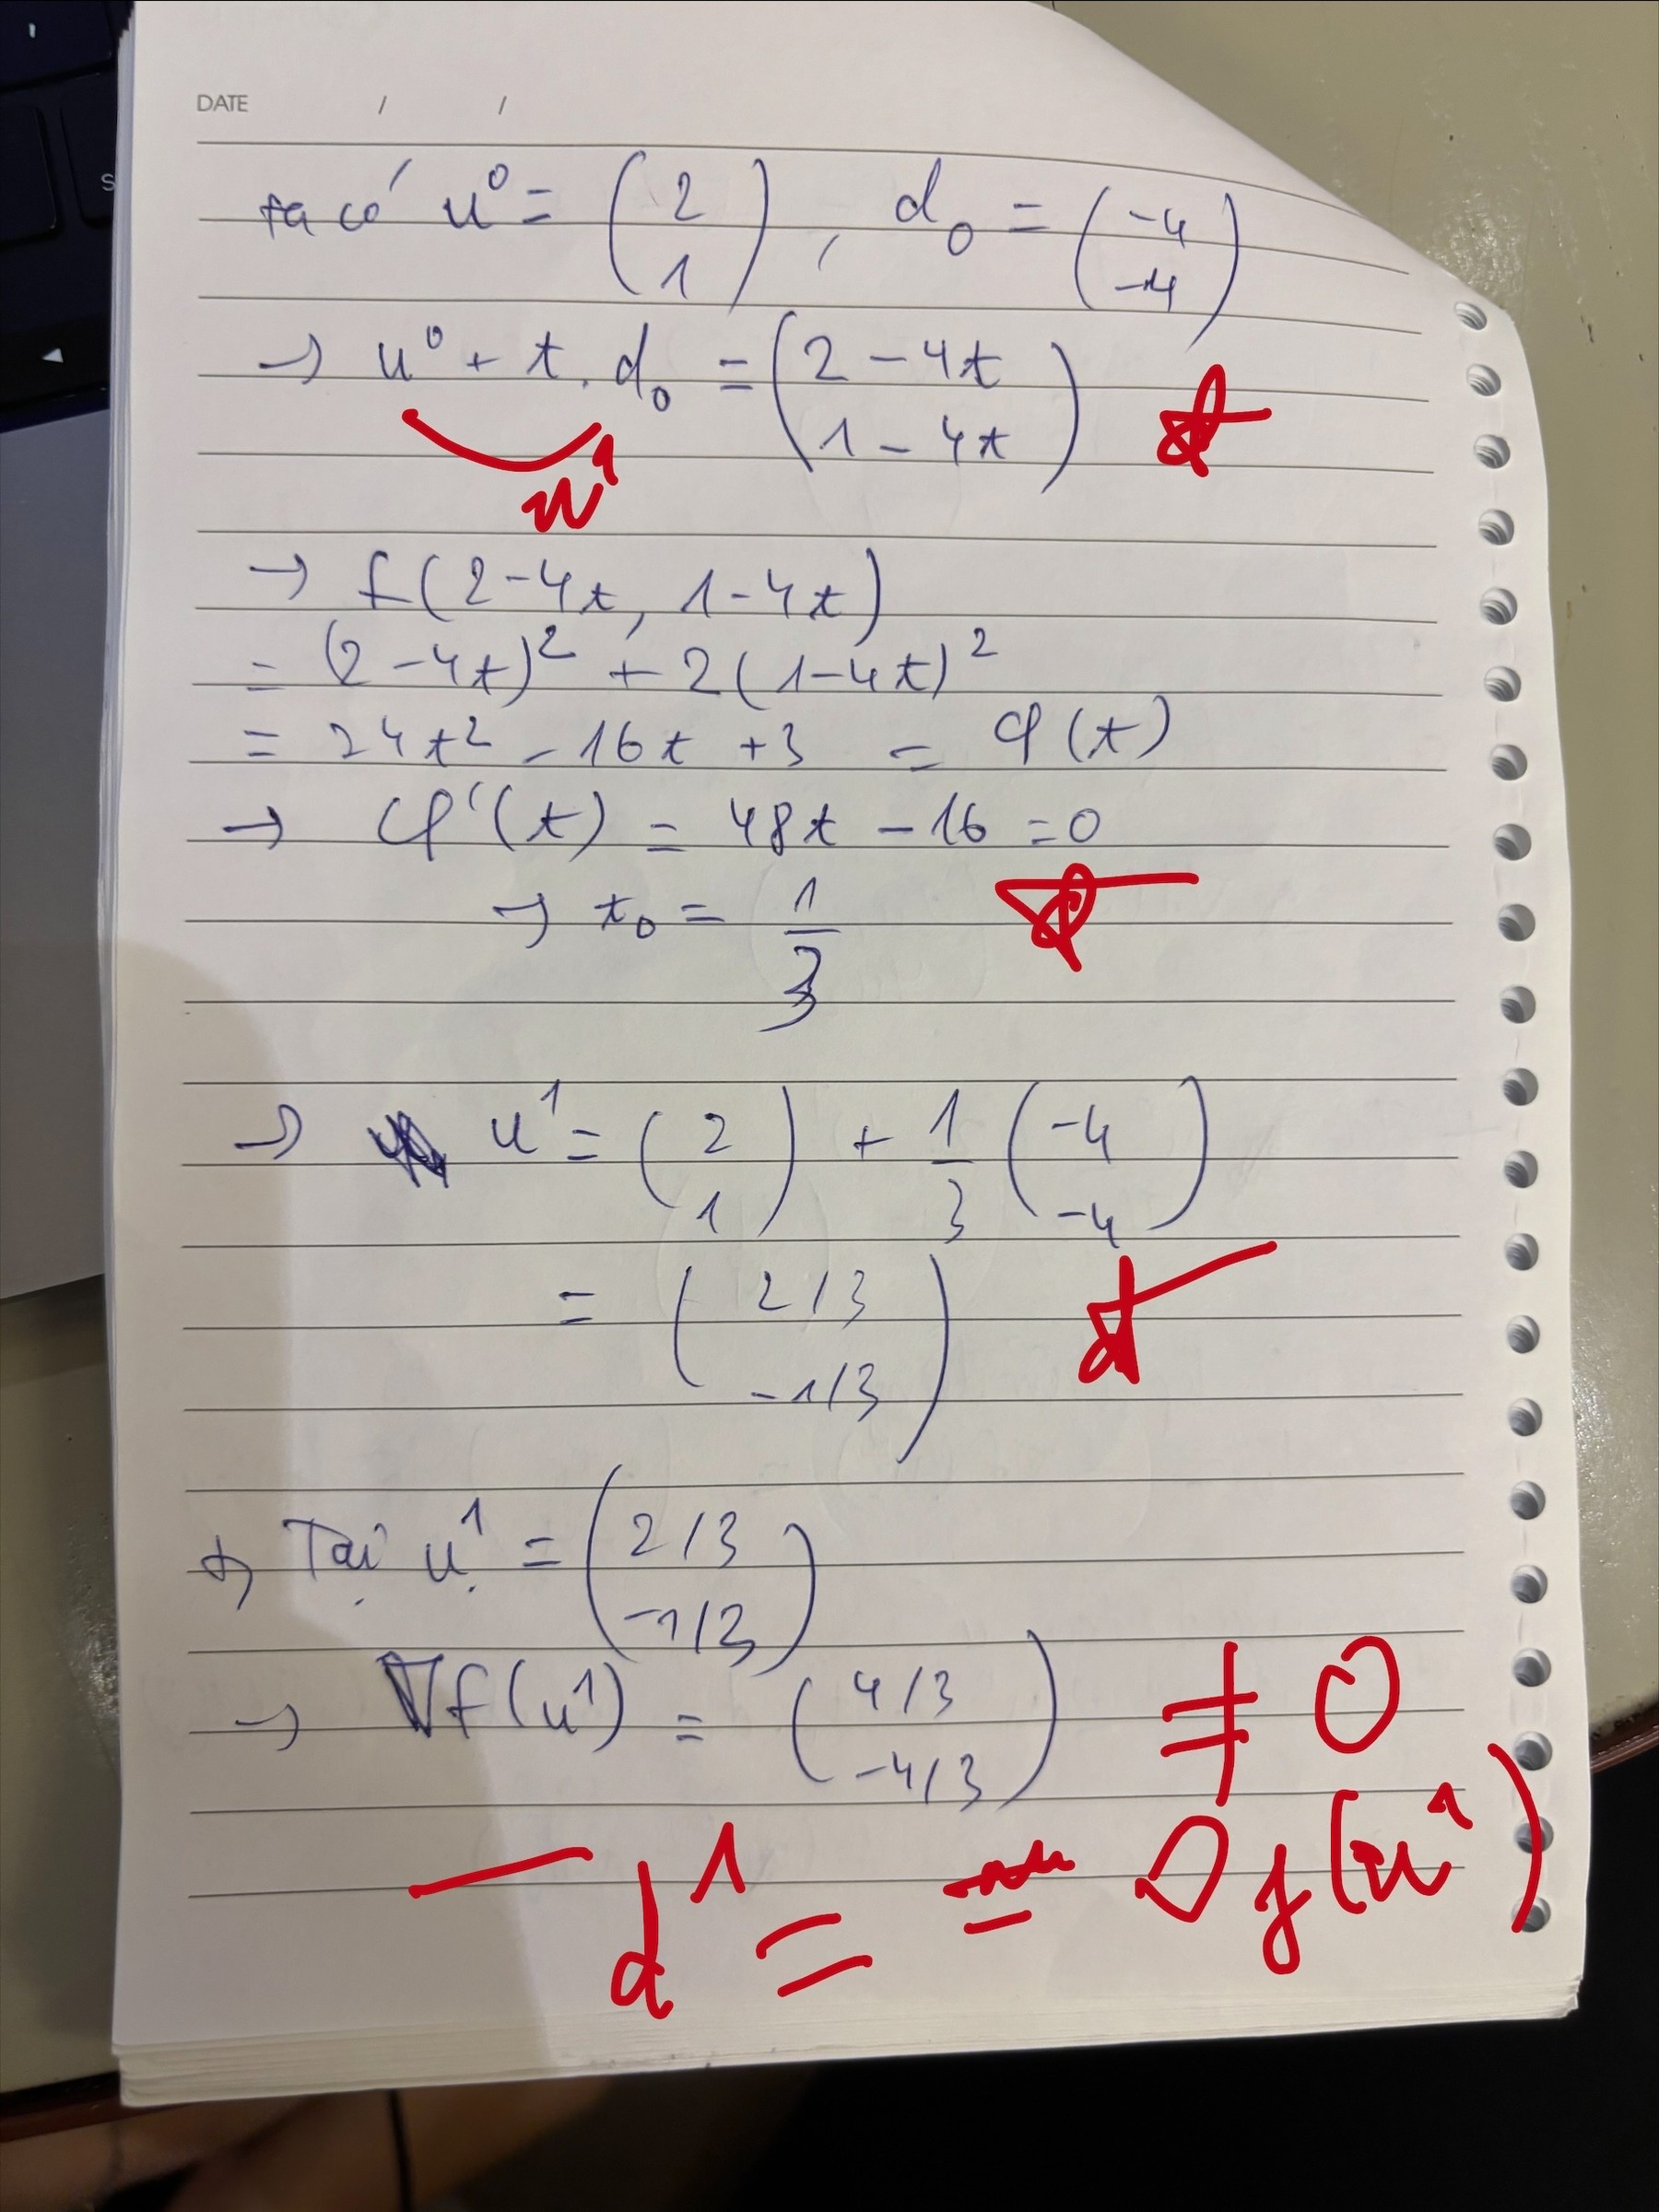
\includegraphics[width=.98\textwidth,height=.82\textheight,keepaspectratio]{bai_lam_them_1_assets/page-089.jpg}\end{center}
\clearpage
\phantomsection\label{src:090}
\noindent\textbf{Ảnh nguồn 090}\par\medskip
\begin{center}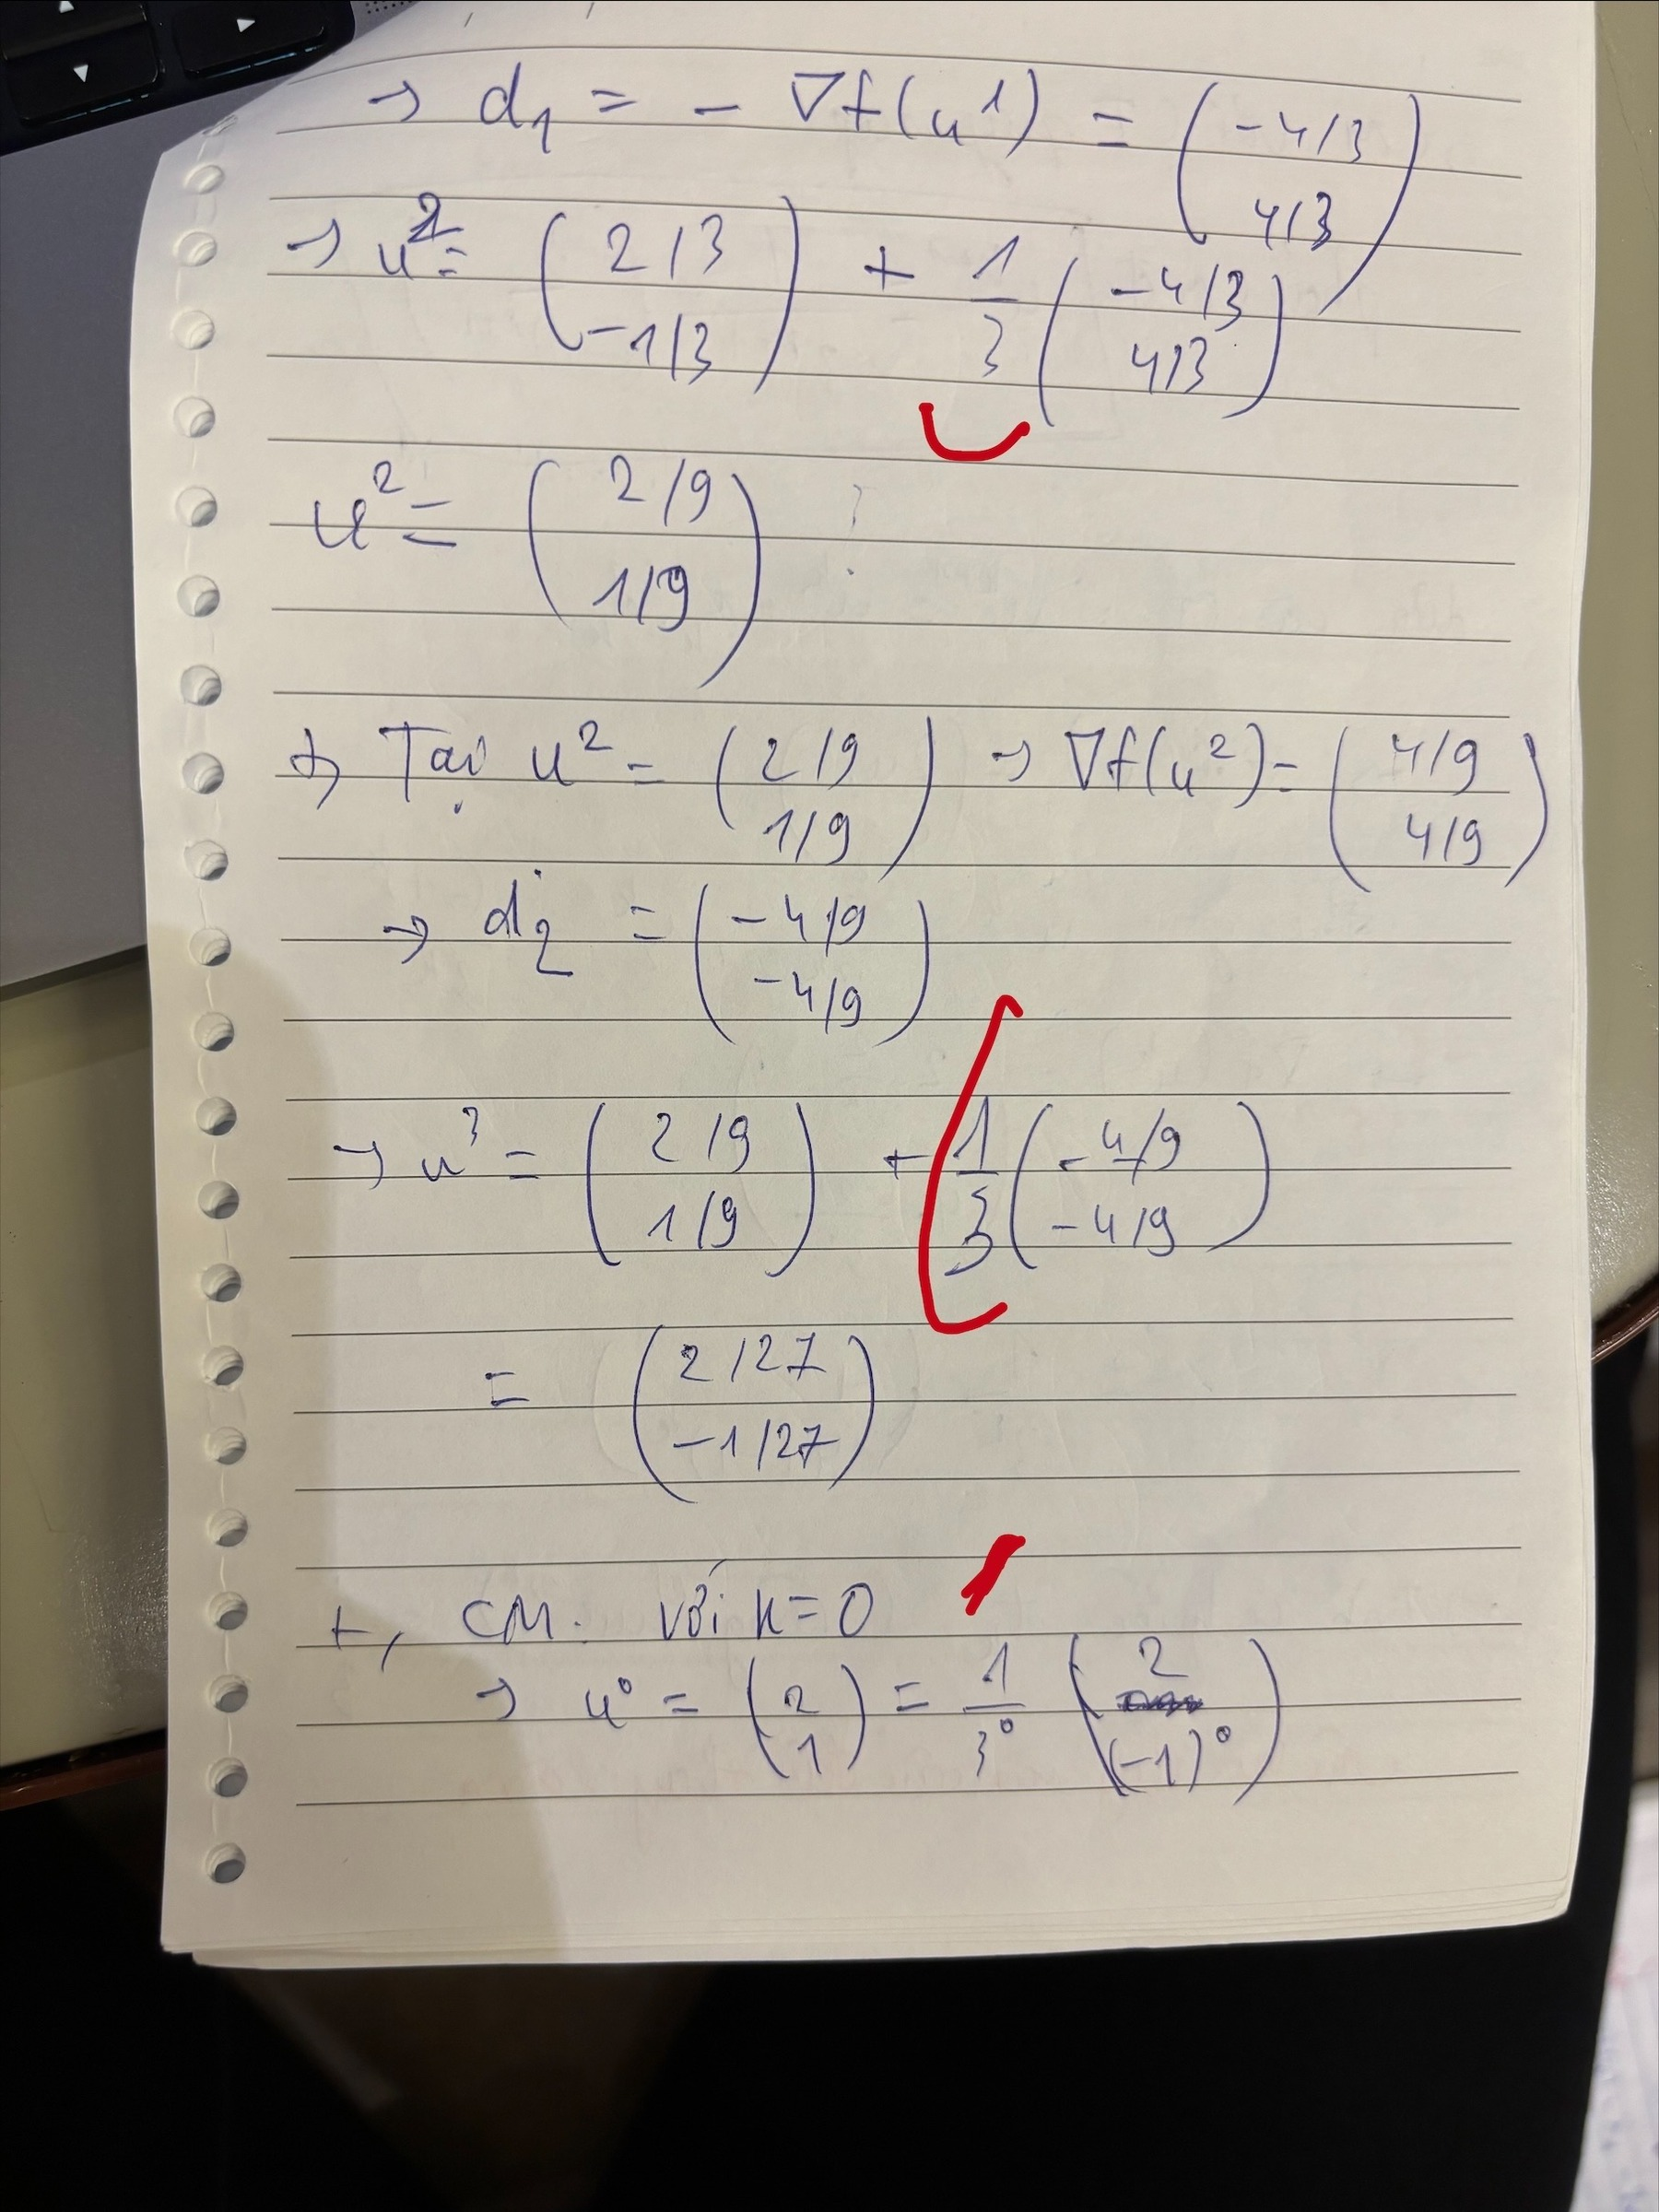
\includegraphics[width=.98\textwidth,height=.82\textheight,keepaspectratio]{bai_lam_them_1_assets/page-090.jpg}\end{center}
\clearpage
\phantomsection\label{src:091}
\noindent\textbf{Ảnh nguồn 091}\par\medskip
\begin{center}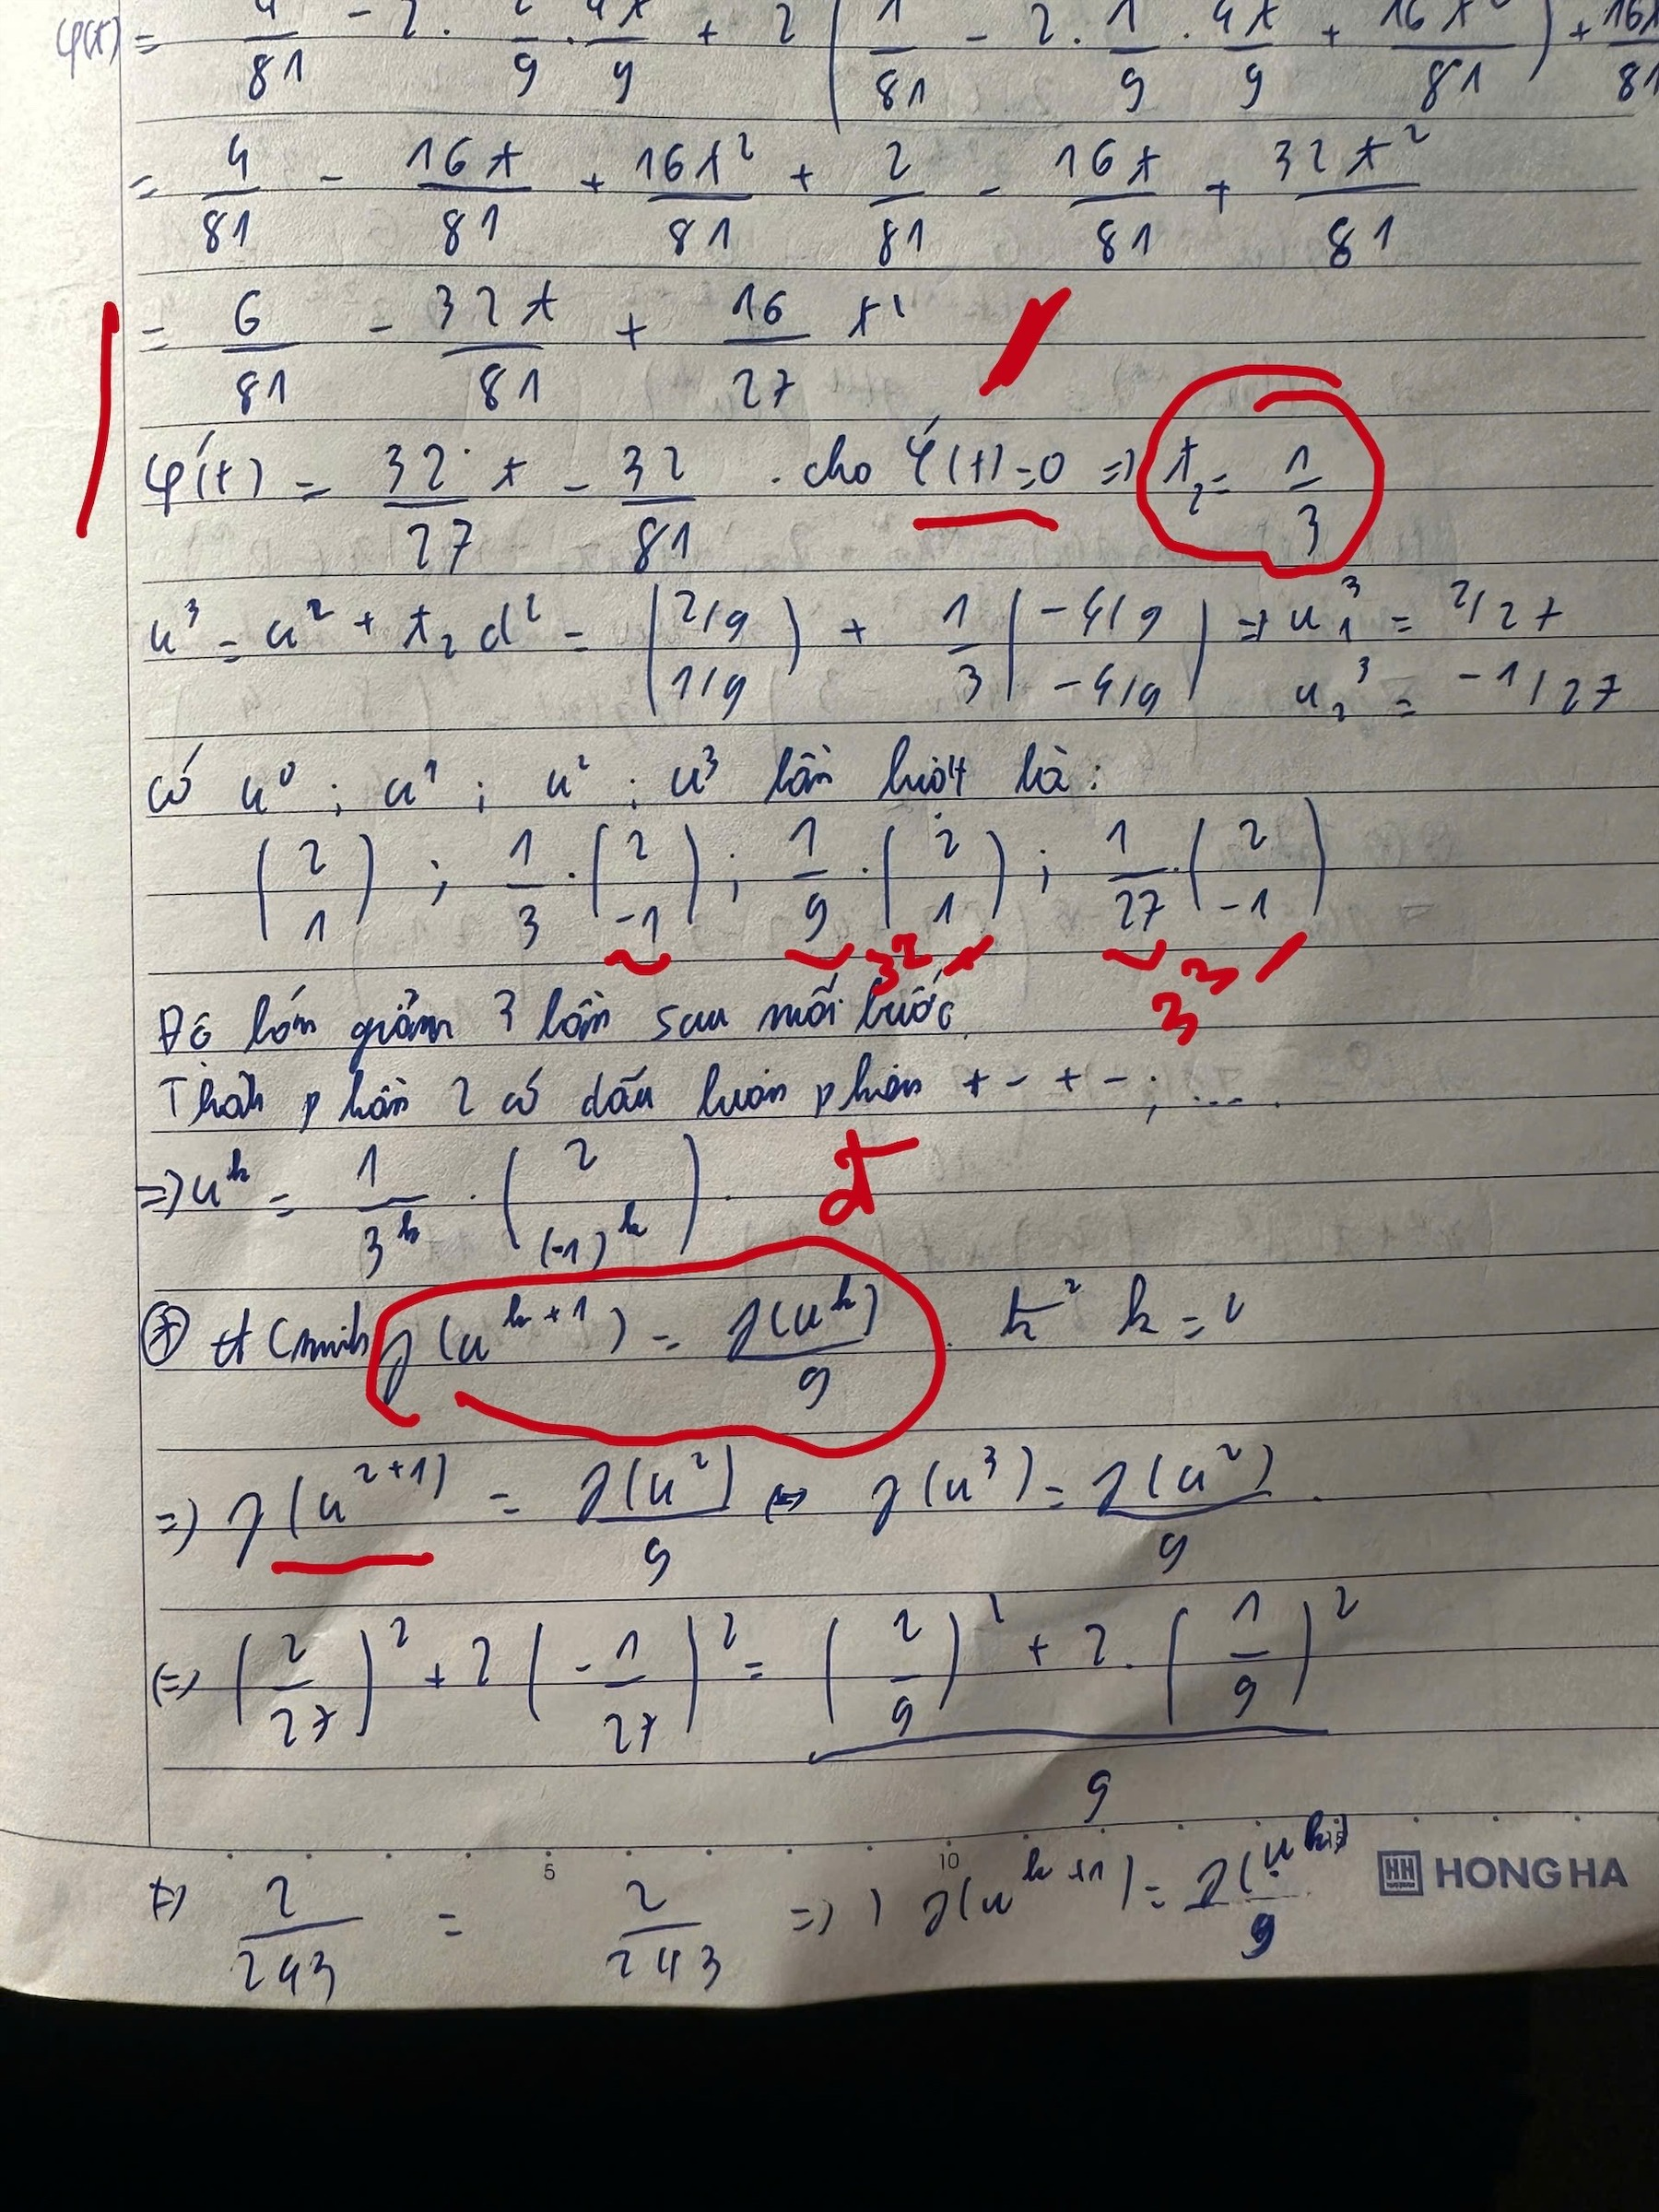
\includegraphics[width=.98\textwidth,height=.82\textheight,keepaspectratio]{bai_lam_them_1_assets/page-091.jpg}\end{center}
\clearpage
\phantomsection\label{src:092}
\noindent\textbf{Ảnh nguồn 092}\par\medskip
\begin{center}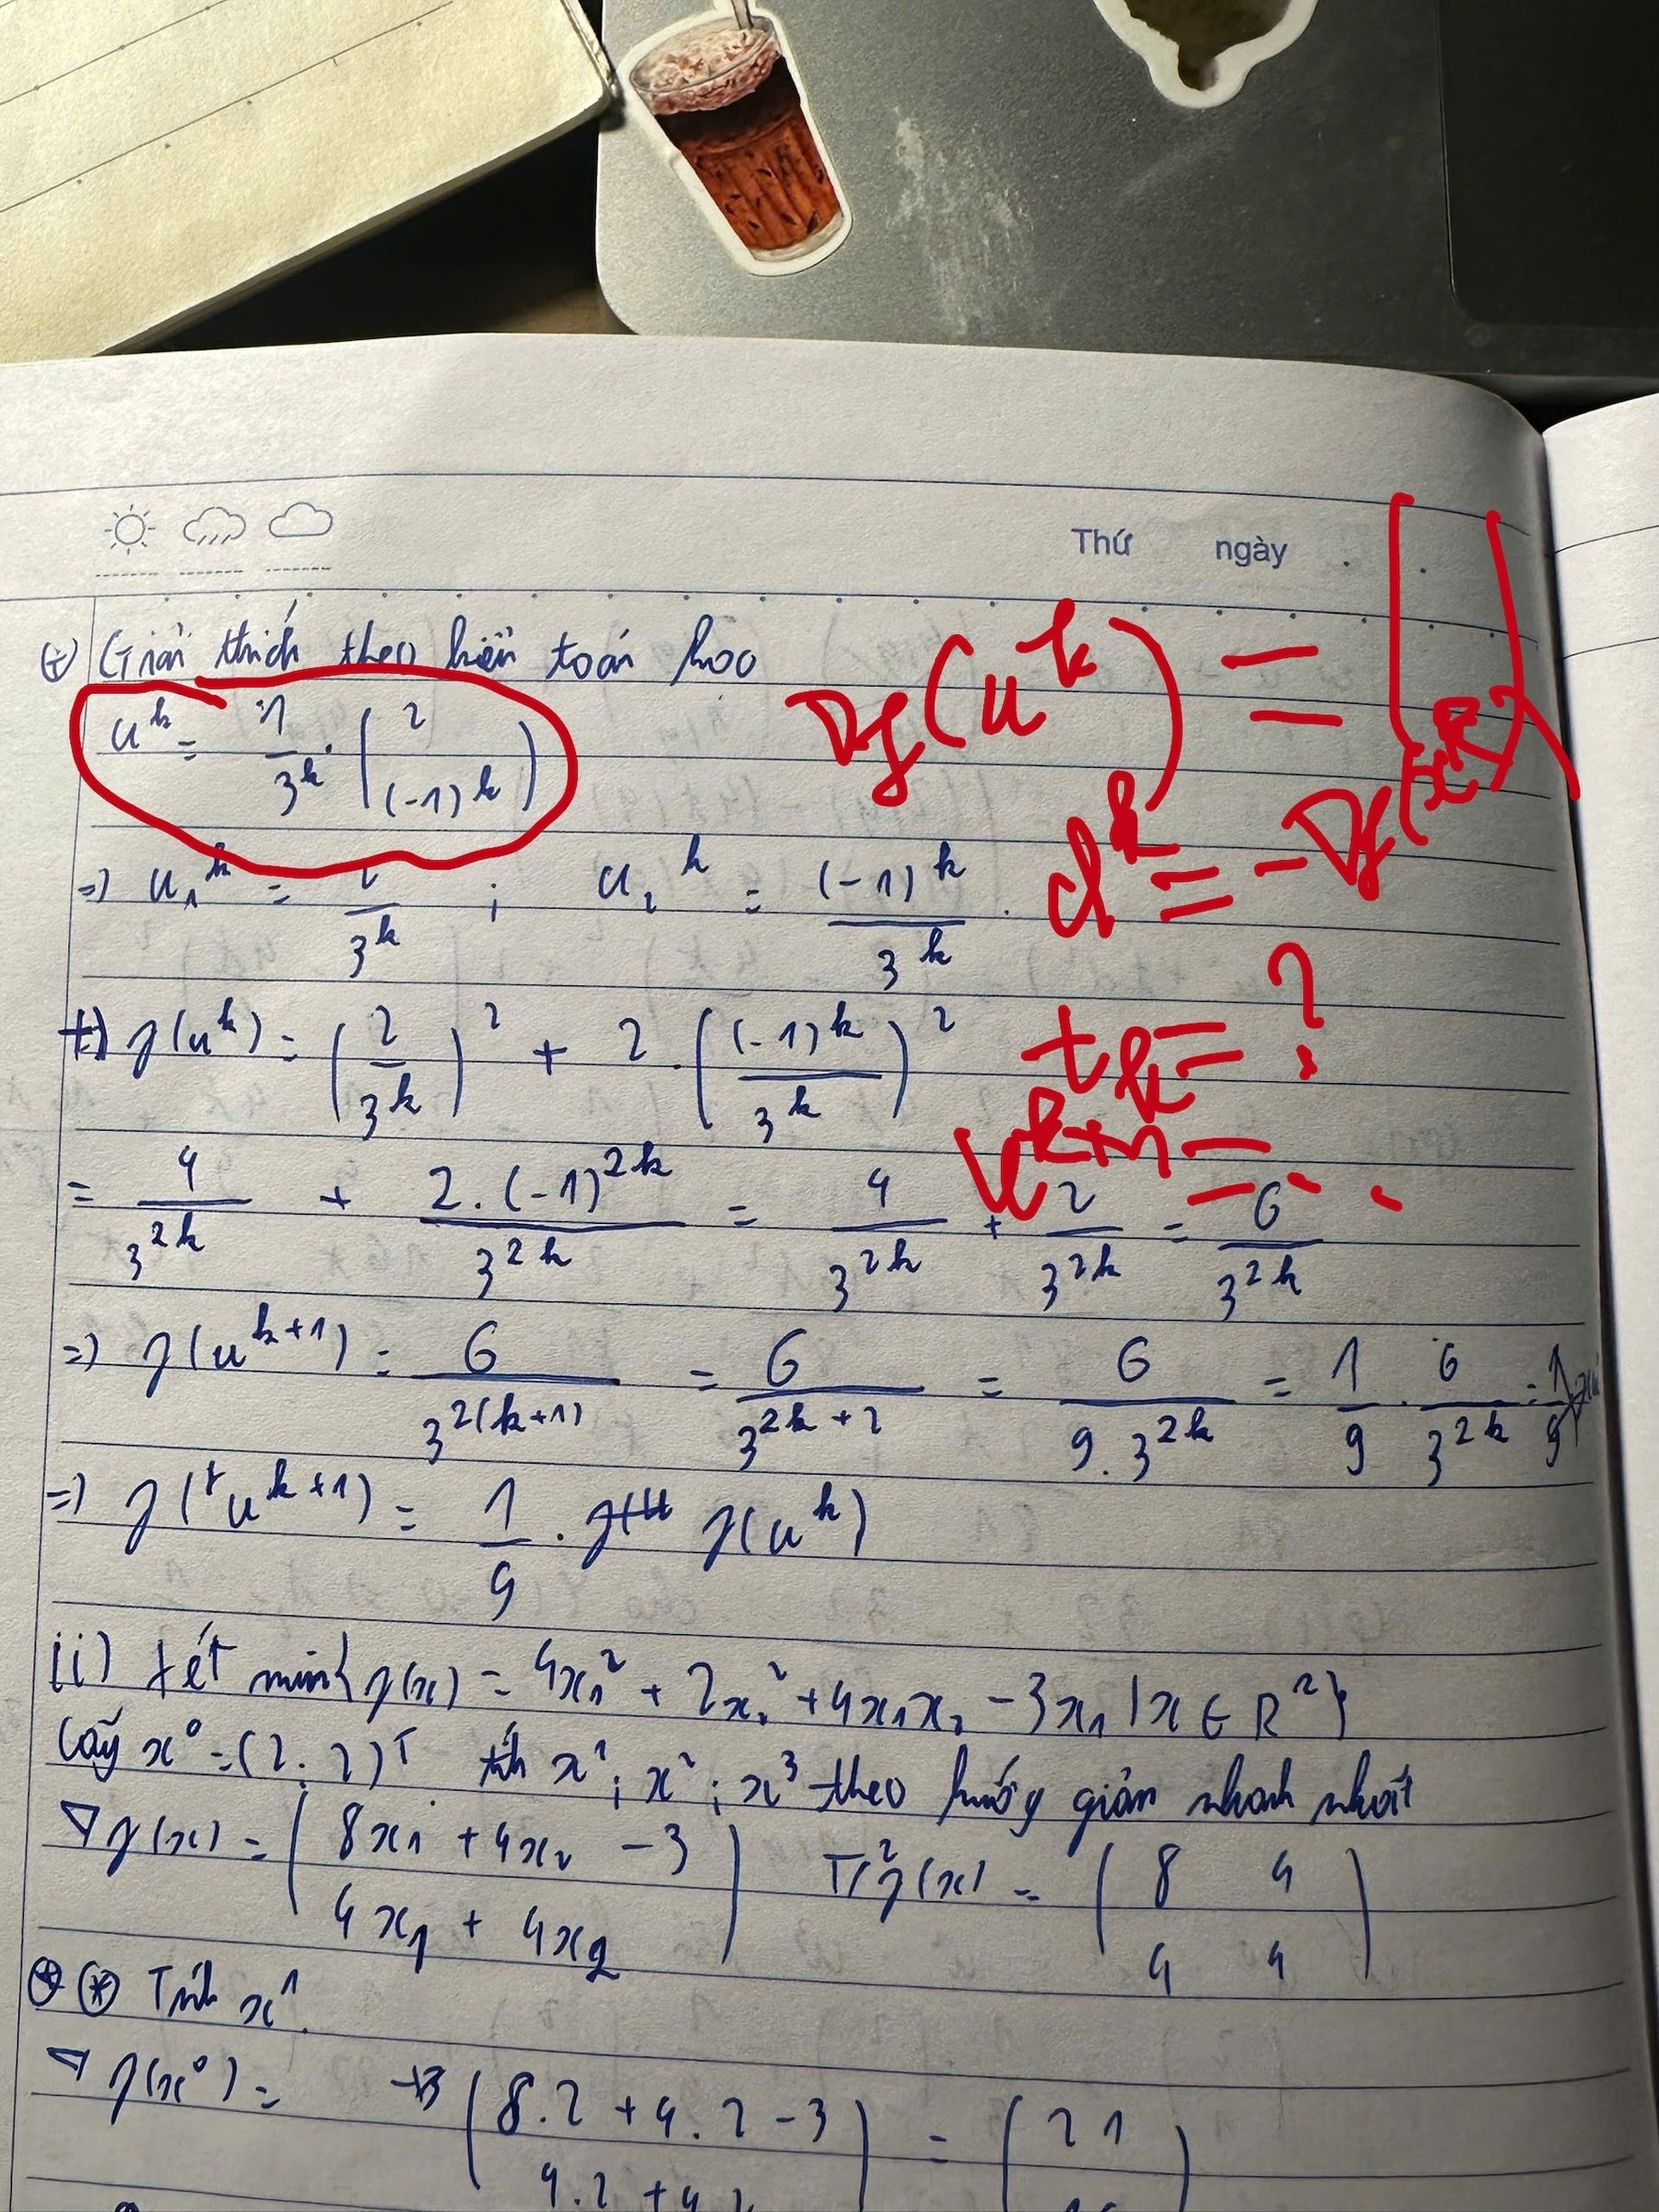
\includegraphics[width=.98\textwidth,height=.82\textheight,keepaspectratio]{bai_lam_them_1_assets/page-092.jpg}\end{center}
\clearpage
\phantomsection\label{src:093}
\noindent\textbf{Ảnh nguồn 093}\par\medskip
\begin{center}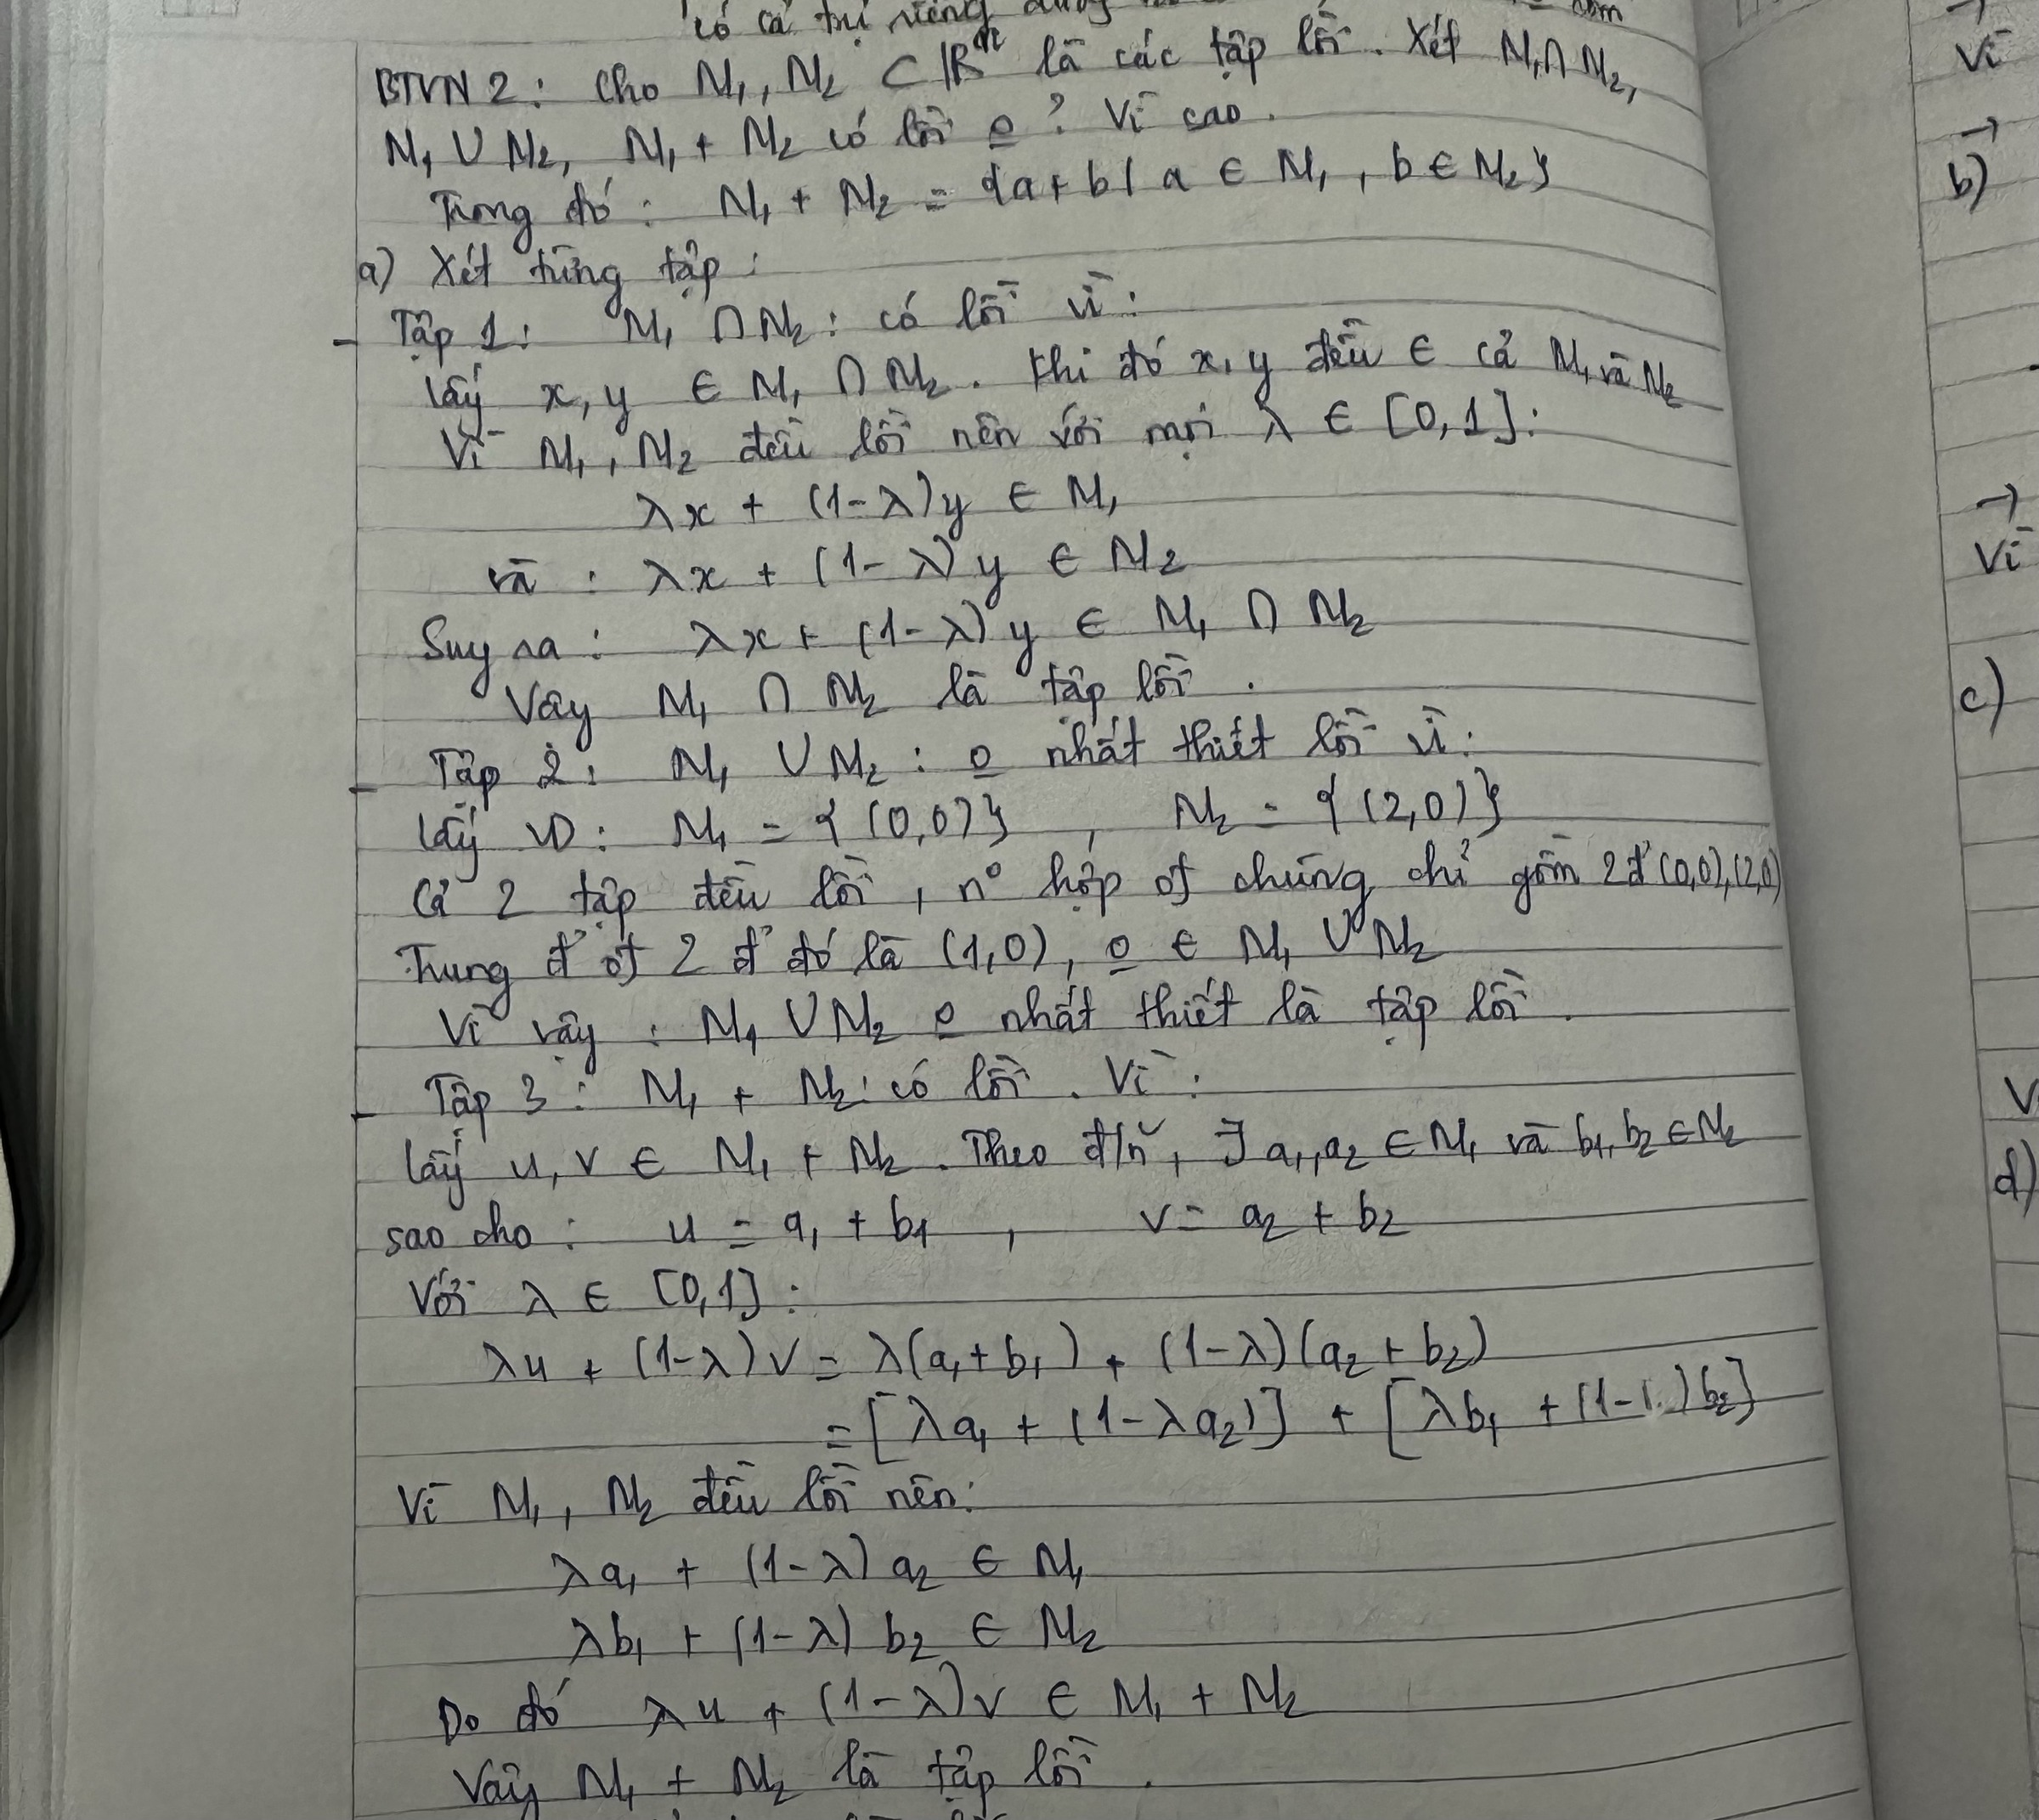
\includegraphics[width=.98\textwidth,height=.82\textheight,keepaspectratio]{bai_lam_them_1_assets/page-093.jpg}\end{center}
\clearpage
\phantomsection\label{src:094}
\noindent\textbf{Ảnh nguồn 094}\par\medskip
\begin{center}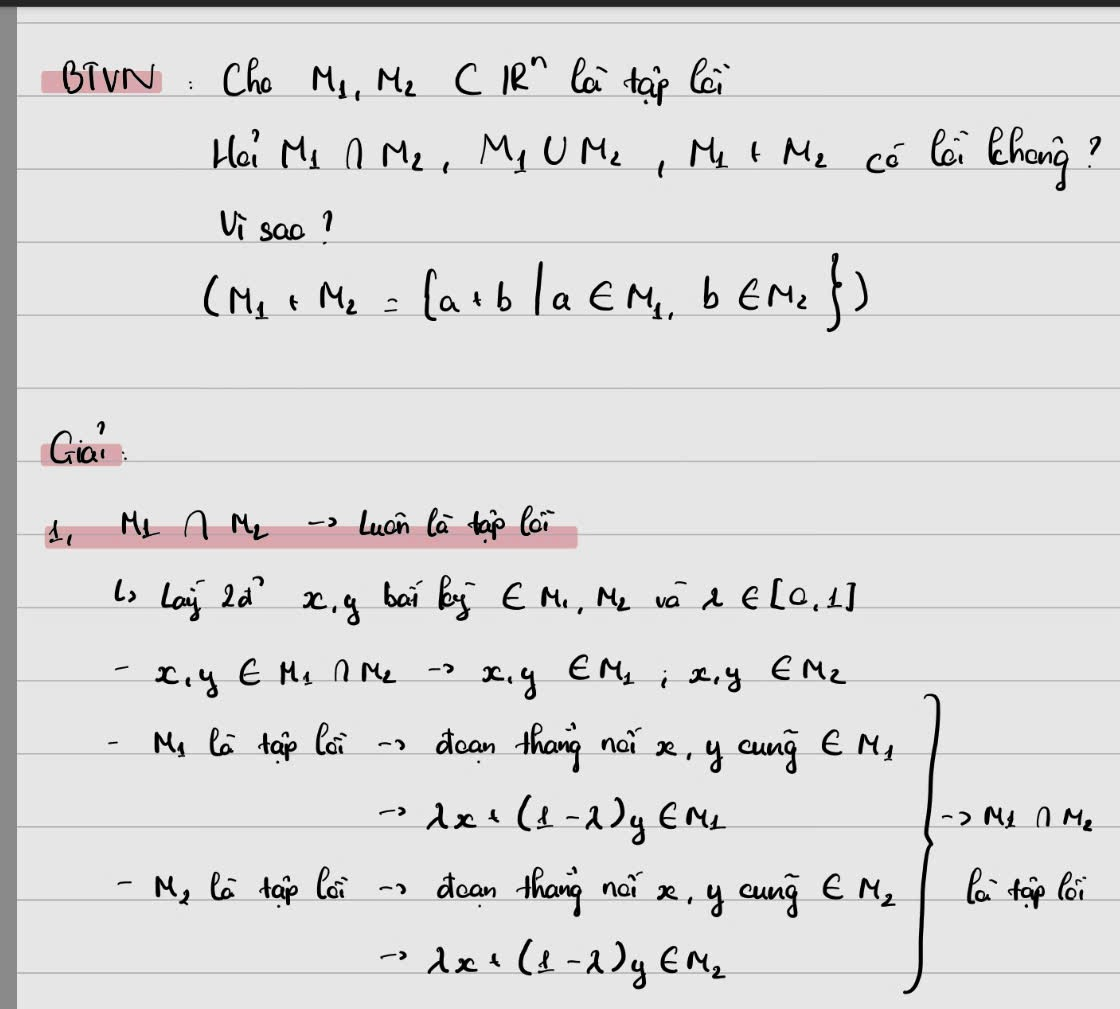
\includegraphics[width=.98\textwidth,height=.82\textheight,keepaspectratio]{bai_lam_them_1_assets/page-094.jpg}\end{center}
\clearpage
\phantomsection\label{src:095}
\noindent\textbf{Ảnh nguồn 095}\par\medskip
\begin{center}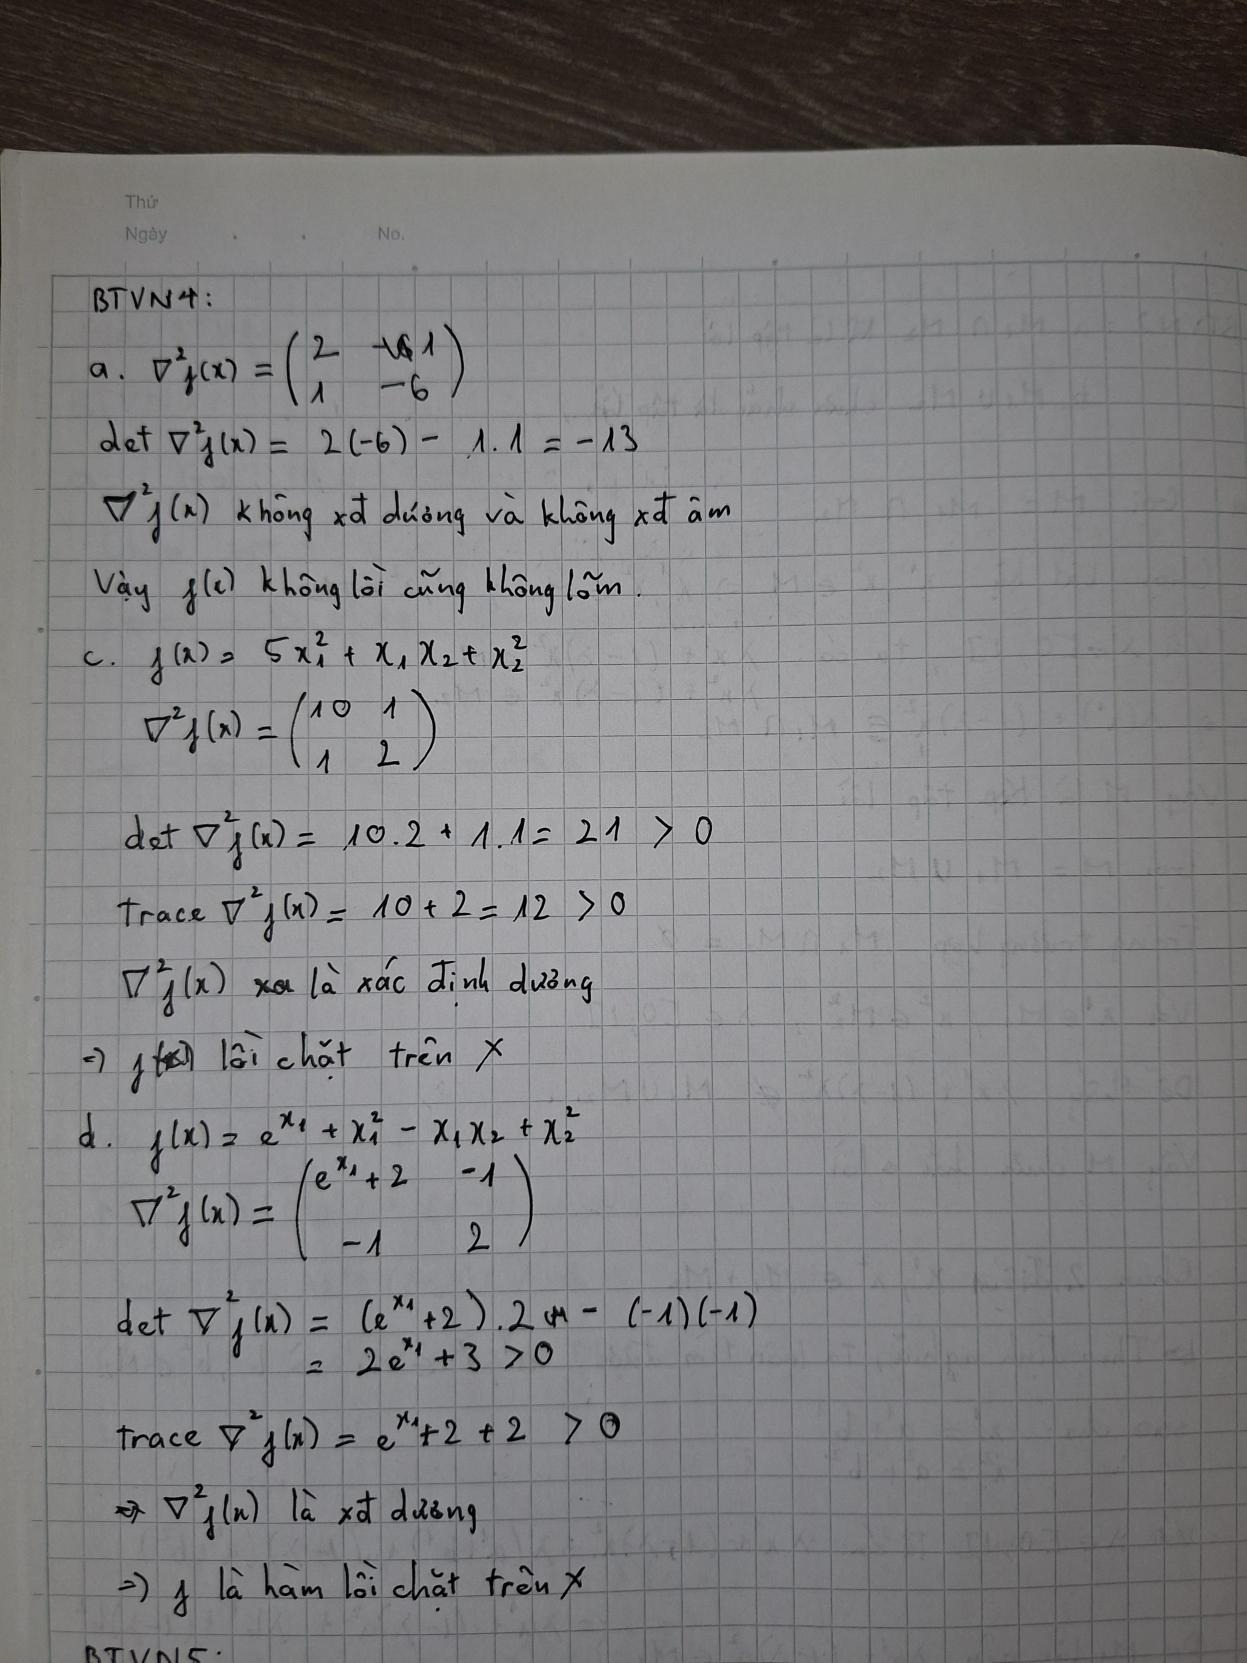
\includegraphics[width=.98\textwidth,height=.82\textheight,keepaspectratio]{bai_lam_them_1_assets/page-095.jpg}\end{center}
\clearpage
\phantomsection\label{src:096}
\noindent\textbf{Ảnh nguồn 096}\par\medskip
\begin{center}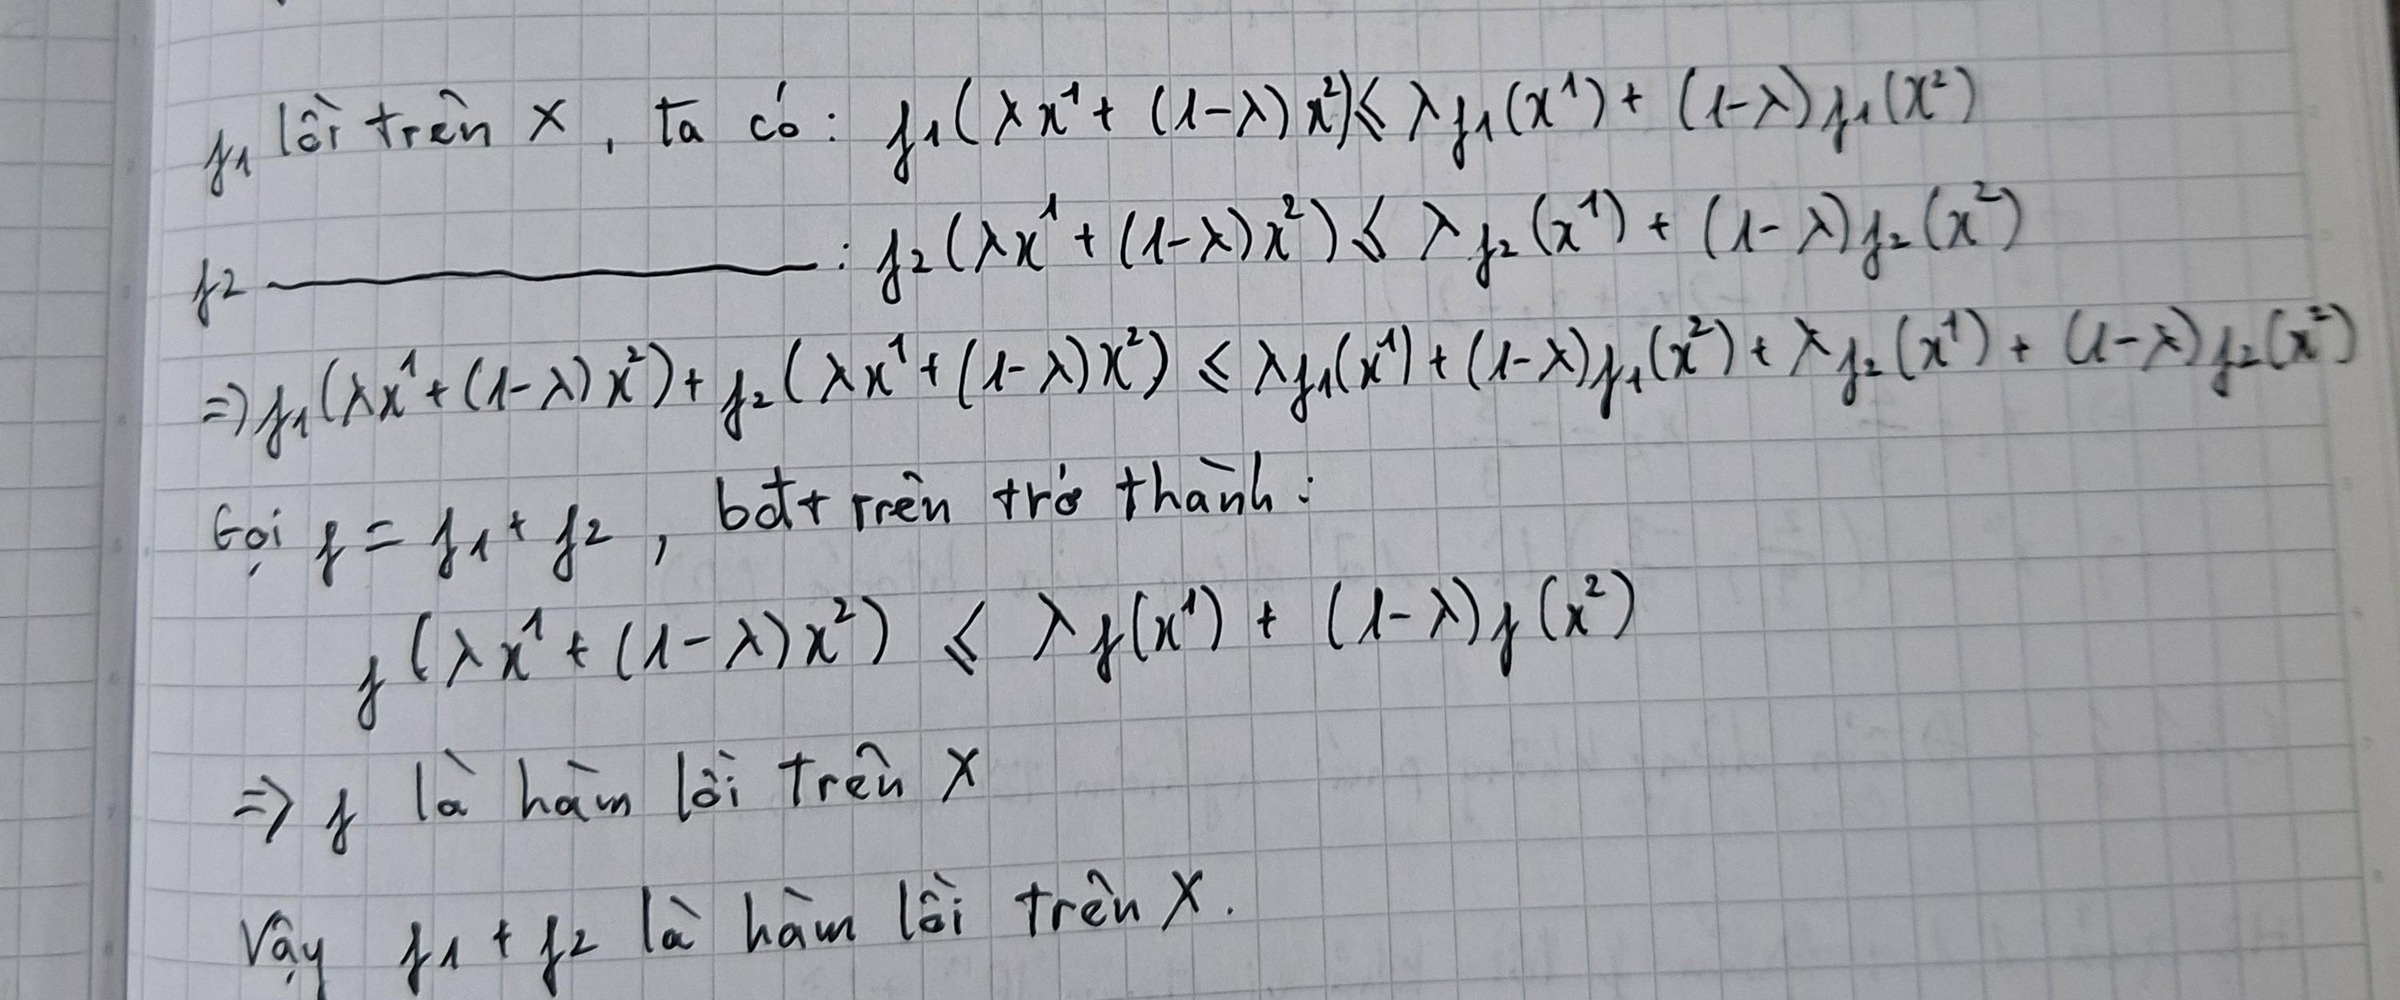
\includegraphics[width=.98\textwidth,height=.82\textheight,keepaspectratio]{bai_lam_them_1_assets/page-096.jpg}\end{center}
\clearpage
\phantomsection\label{src:097}
\noindent\textbf{Ảnh nguồn 097}\par\medskip
\begin{center}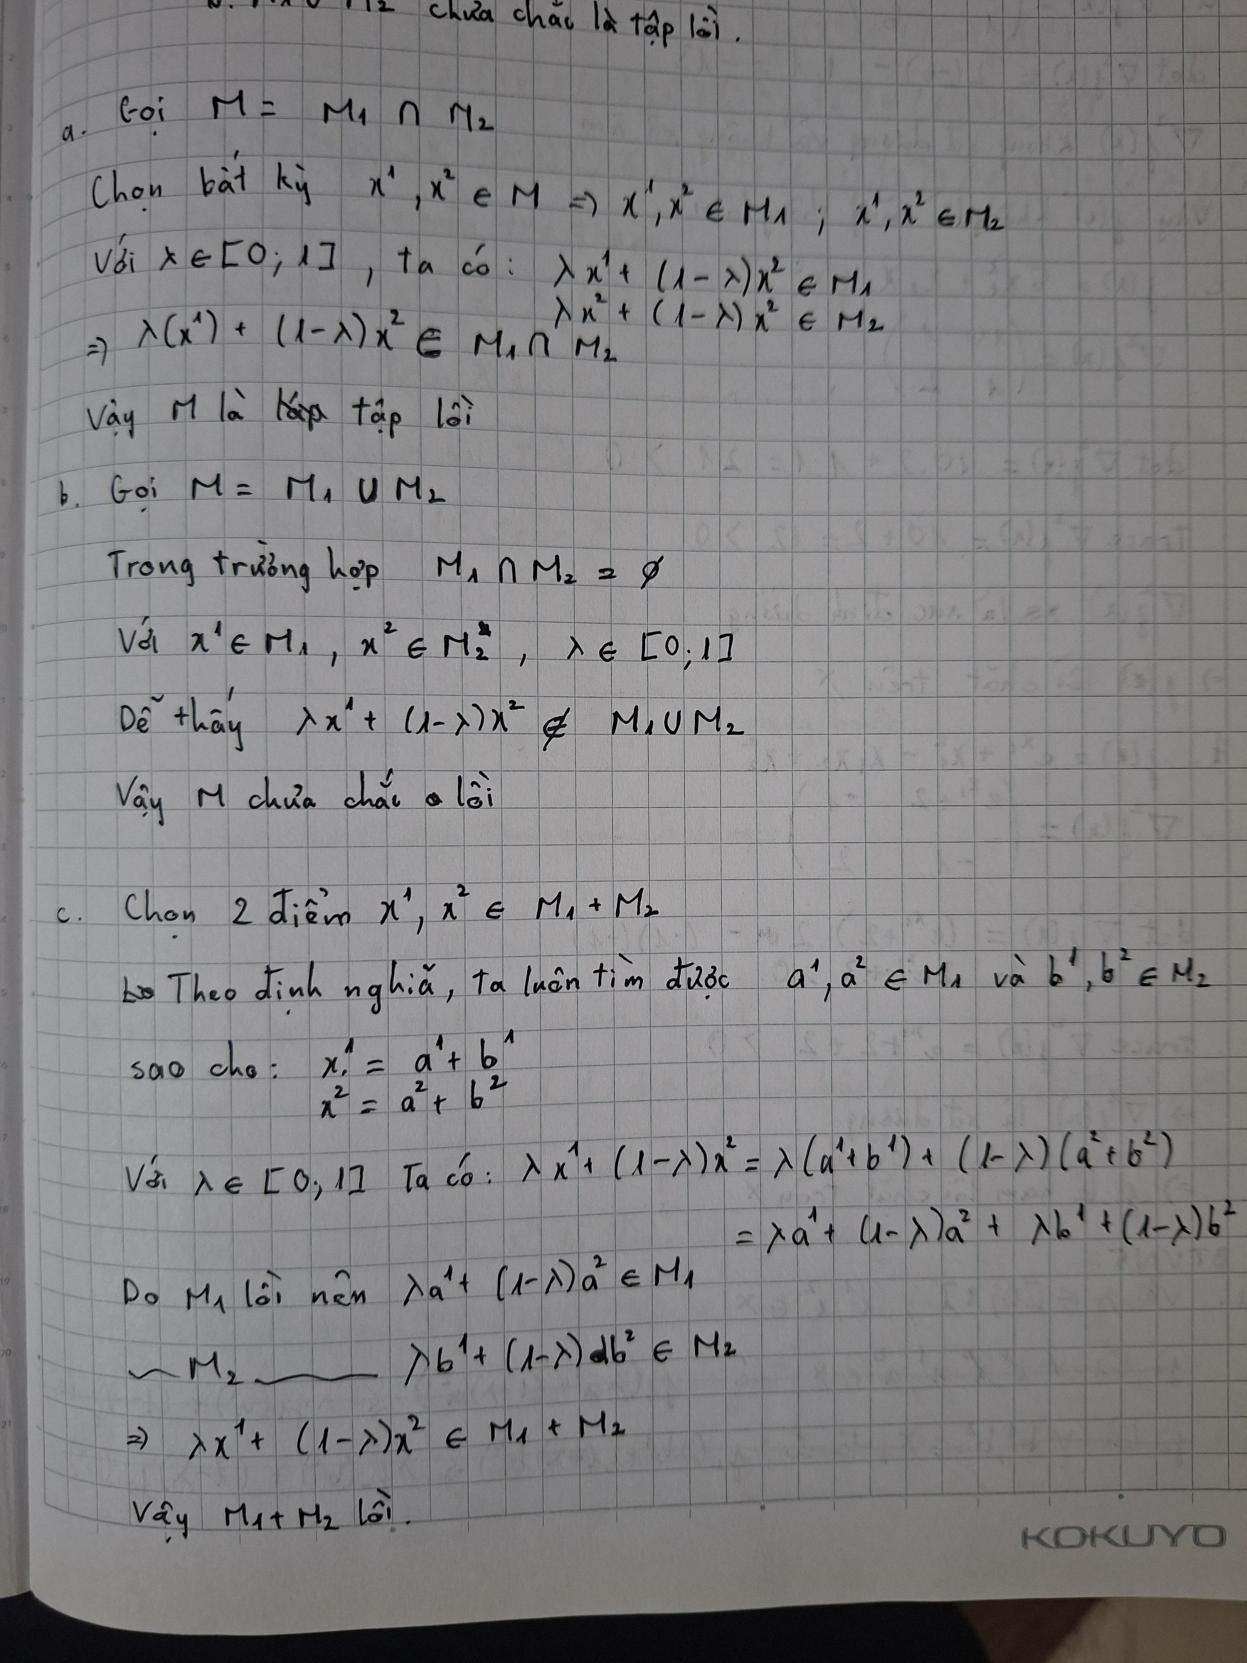
\includegraphics[width=.98\textwidth,height=.82\textheight,keepaspectratio]{bai_lam_them_1_assets/page-097.jpg}\end{center}


\end{document}
